%%%%%%%%%%%%%%%%%%%%%%%%%%%%%%%
% Inlcude preable
%%% Definition der Dokumentklasse für A4-Papier und 12 Punkte Schriftgröße.
%%% Ränder sind für Klebebindung sowohl im A4- als auch im herunterskalierten
%%% A5-Ausdruck optimiert.
\documentclass[a4paper,titlepage,bibliography=totoc,12pt,BCOR17mm,DIV12,headinclude,footinclude=false]{scrbook}

\usepackage[utf8]{inputenc}

\usepackage{easy-todo}

\usepackage{tikz}
\usetikzlibrary{decorations.markings,decorations.text,calc,arrows,positioning,shapes}
\tikzstyle{decision} = [diamond, draw, fill=blue!20, text width=4.5em, text badly centered, node distance=2cm, inner sep=0pt]
\tikzstyle{block} = [rectangle, draw, fill=blue!20, text width=0.8\textwidth, text centered, rounded corners, minimum height=3em]
\tikzstyle{block2} = [rectangle, draw, text centered, rounded corners, minimum height=2em]
\tikzstyle{line} = [draw, -latex']
\tikzstyle{cloud} = [draw, ellipse,fill=red!20, node distance=3cm, minimum height=2em]
\tikzstyle{process} = [rectangle, minimum width=3cm, minimum height=2em, text centered, draw=black, fill=orange!30]

\usepackage{minibox}
\usepackage{mdframed}
\mdfsetup{
  skipabove=\baselineskip,
  skipbelow=\baselineskip
}


%%%%%%%%%%%%%%%%%%%%%%%%%%%%%%
%%% Math symbols etc
\usepackage{amsmath,amsfonts,amssymb}
\usepackage{bbold}
\usepackage{slashed}
\usepackage{physics}
\usepackage{booktabs}
\usepackage{tabularx,bigdelim}
\usepackage{multirow}
\usepackage{xfrac}
\usepackage{siunitx}
\usepackage{mathtools}

%%%%%%%%%%%%%%%%%%%%%%%%%%%%%%
%%% Grafics
\usepackage{graphicx}
\usepackage{caption}
%\usepackage{subcaption}
%%% Sidecap: Bildbeschriftung seitlich neben dem Bild
%\usepackage{sidecap}
\usepackage[caption=false]{subfig}

\usepackage{placeins}
\usepackage{adjustbox}

%%%%%%%%%%%%%%%%%%%%%%%%%%%%%%
%%% Header
%%% Fancyhdr: Nette Kopf- und Fusszeilen, werden weiter unten definiert.
\usepackage{fancyhdr}
%%% Definition der Kopf- und Fussleisten
\pagestyle{fancy}
\renewcommand{\chaptermark}[1]{% Kopfzeilen in Groß-/Kleinschreibung
\markboth{%
\chaptername\ \thechapter.%
\ #1}{}}
\renewcommand{\sectionmark}[1]{% Kopfzeilen in Groß-/Kleinschreibung
\markright{%
\thesection.%
\ #1}}


\usepackage{titlesec, blindtext, color} 

%\definecolor{gray75}{gray}{0.75}
%\newcommand{\hsp}{\hspace{20pt}}
%\titleformat{\chapter}[hang]{\Huge\bfseries}{\thechapter\hsp\textcolor{gray75}{|}\hsp}{0pt}{\Huge\bfseries}

%\renewcommand{\thechapter}{\Roman{chapter}}
\titleformat{\chapter}[display]
{\bfseries\Large}
{\filleft\MakeUppercase{\chaptertitlename} \Huge\thechapter}
{2ex}
{\titlerule
  \vspace{1ex}%
\filright}
[\vspace{2ex}%
\titlerule]

\titlespacing{\chapter}{0cm}{-1cm}{0.5cm}[0cm]

%\titleformat{\chapter}[display]
%  {\bfseries\Large}
%  {\filright\MakeUppercase{\chaptertitlename} \Huge\thechapter}
%  {1ex}
%  {\titlerule\vspace{1ex}\filleft}
%  [\vspace{1ex}\titlerule]

%%% Seitennumerierung vor dem eigentlichen Inhalt in römischen Zahlen
\pagenumbering{roman}

%%% Vermeidung von Hurenkindern und Schusterjungen
\clubpenalty = 10000  % schliesst Schusterjungen aus
\widowpenalty = 10000 % schliesst Hurenkinder aus


%%%%%%%%%%%%%%%%%%%%%%%%%%%%%%
%%% Einige Pakete für eine schöne Titelseite
\usepackage{everyshi,eso-pic,calc,ifthen,sty/wallpaper}
\usepackage{sty/diplomarbeit}

%%%%%%%%%%%%%%%%%%%%%%%%%%%%%%

%%% Eineinhalbfachen Zeilenabstand nutzen (Vorgabe Prüfungsamt)
\usepackage{setspace}
%\onehalfspacing
\typearea[current]{last}



\usepackage[%
  pdftitle={Scattering Amplitudes with Multi-Loop Generalized Numerical Unitarity Method},%
  pdfauthor={Vasily Sotnikov}%
]{hyperref}

\hypersetup{
    colorlinks=true,
    allcolors={blue!60!black}
    %linkcolor={red!50!black},
    %citecolor={blue!50!black},
    %urlcolor={blue!80!black}
}

%%% Mehrere aufeinanderfolgend numerierte Zitate mit einem Bindestrich zusammen
%%% fassen (z.B. [1-5] statt [1,2,3,4,5]).
\usepackage[numbers,sort&compress]{natbib}
\usepackage{doi}
%\usepackage{mcite}

%%% Hypernat beseitigt Fehler durch das
%%% Paket Hyperref in Zusammenhang mit dieser Kompression.
%\usepackage{hypernat}


%%%%%%%%%%%%%%%%%%%%%%%%%%%%%%

%-- Defines a CAPTION for a set of equations and numbers
%   the set of equations is numbered
% note: the caption adapts the text alignment to the length. 
\newcounter{captionedequationset} %numbering
\newdimen\captionlength
\newcommand{\captionedequationset}[1]{
    \refstepcounter{figure}% Step counter
    \setlength{\captionlength}{\widthof{#1}} %
    \addtolength{\captionlength}{\widthof{Figure~\thefigure: }}
    %If the caption is shorter than the line width then
    % the caption is centred, otherwise is flushed left.
    \ifthenelse{\lengthtest{\captionlength < \linewidth }} %
    {\begin{center}
            Figure~\thefigure: #1
        \end{center}} 
    { \begin{flushleft} 
        Figure~\thefigure: #1 %
        \end{flushleft}}}




%%%%%%%%%%%%%%%%%%%%%%%%%%%%%%
%%%%%%%%%%%%%%%%%%%%%%%%%%%%%%
%  NOT USE CURRENTLY
%%%%%%%%%%%%%%%%%%%%%%%%%%%%%%
%%%%%%%%%%%%%%%%%%%%%%%%%%%%%%
%%% Fancyref: Vereinfachte Referenzen. Labels werden im Format "PRÄFIX:LABEL"
%%%           erstellt. Dann wird mit \fref{PRÄFIX:LABEL} ein Verweis der Form
%%%           z.B. "Kapitel 4" oder "Abschnitt 4.5" statt nur "4" oder "4.5"
%%%           erstellt.
%%%           ACHTUNG: Fehlt im Label im \fref-Kommando das Präfix und der
%%%           Doppelpunkt, kommt es zu Fehlermeldungen, die ein fehlendes "}"
%%%           beklagen!
%%%           Liste der Präfixe und zugehöriger Objekte:
%%%           Object      Prefix
%%%           Chapter     chap
%%%           Section     sec
%%%           Equation    eq
%%%           Figure      fig
%%%           Table       tab
%%%           Enumeration enum
%%%           Footnote    fn
%%%           Anhang*     apx
%%%           *) Selbst definiertes Präfix

%%%\usepackage[german,plain]{fancyref}
%%% 
%%%\newcommand*{\fancyrefapxlabelprefix}{apx}
%%%\frefformat{plain}{\fancyrefapxlabelprefix}{%
%%%    Anhang\fancyrefdefaultspacing#1%
%%%}%
%%%\Frefformat{plain}{\fancyrefapxlabelprefix}{%
%%%    Anhang\fancyrefdefaultspacing#1%
%%%}%

%%%%%%%%%%%%%%%%%%%%%%%%%%%%%%
%%% URL: Zur besseren Darstellung von URLs z.B. in Literaturquellen (einbindbar
%%%      z.B. über "howpublished = \url{URL}")
%\usepackage{url}

%%%%%%%%%%%%%%%%%%%%%%%%%%%%%%
%%% Hyphenat: Problemlöser für Trennungsprobleme: TeX trennt keine Wörter, die
%%%           bereits einen Bindestrich beinhalten (z.B. Wasserstoff-Atom).
%%%           Um die automatische Worttrennung auch bei solchen Wörtern zu 
%%%           aktivieren, ersetzt man einfach den Bindestrich durch das 
%%%           Kommando \hyp{}, also z.B. "Wasserstoff\hyp{}Atom".
%\usepackage{hyphenat}

%%%%%%%%%%%%%%%%%%%%%%%%%%%%%%

%%% Mit diesen Kommandos kann man eigene Kapitel- und Sektionskopfzeilen
%%% einbinden. Anwendung:
%%%    \chapter{Langer Kapitelname}
%%%    \shortchapter{Kurzer Kapitelname für Kopfzeile}
%\newcommand{\shortchapter}[1]{% Erstellt eine eigene Kapitel-Kopfzeile
%\markboth{%
%\chaptername\ \thechapter.%
%\ #1}{}}
%\newcommand{\shortsection}[1]{% Erstellt eine eigene Sektions-Kopfzeile
%\markright{%
%\thesection.%
%\ #1}}

%%%%%%%%%%%%%%%%%%%%%%%%%%%%%%

\usepackage{cmap}
\usepackage{indentfirst}

% for ranges of equations
\usepackage{cleveref}

\graphicspath{{figures/}}


%%%%%%%%%%%%%%%%%%%%%%%%%%%%%%
% Own defs etc
%----------------------------------------------------------------------------------------------
\textheight = 24cm
\textwidth = 16cm
\oddsidemargin = -5pt
\topmargin = -1.5cm
\parskip = 10pt
%----------------------------------------------------------------------------------------------
%\numberwithin{equation}{section}
%----------------------------------------------------------------------------------------------


\def\recola{\texttt{RECOLA}}
\def\OL{\texttt{OpenLoops}}
%\def\BH{\texttt{BlackHat}}
\renewcommand{\textfraction}{0}
\renewcommand{\topfraction}{1}
\renewcommand{\bottomfraction}{1}
\newcommand{\BlackHat}{\texttt{BlackHat}}
%\newcommand{\BHM}{{\textsc BlackHat\textunderscore Massive}}
\newcommand{\PYTHIA}{\textsc{Pythia}}
\newcommand{\HELACNLO}{\textsc{HELAC-NLO}}
\newcommand{\NLOJet}{\textsc{NLOJET++}}
\newcommand{\SHERPA}{\texttt{SHERPA}}
\newcommand{\MCFM}{\texttt{MCFM}}
\newcommand{\AMEGIC}{\texttt{AMEGIC++}}
\newcommand{\COMIX}{\texttt{COMIX}}
\newcommand{\SISCone}{\texttt{SISCone}}
\newcommand{\ntuple}{{$n$-tuple}}
\newcommand{\ntuples}{{$n$-tuples}}
\newcommand{\Ntuple}{{$N$-tuple}}
\newcommand{\Ntuples}{{$N$-tuples}}
\newcommand{\mc}[1]{\mathcal{#1}}
\newcommand{\FO}{{4FNS}}
\newcommand{\FI}{{5FNS}}

\newcommand{\Abs}[1]{\vert #1 \vert^2}
\newcommand{\Ree}[2]{2\Re({#1}^{*} #2)}


\def\gjn{$\gamma\,\!+\,n$}
\def\jet{{\textrm jet}}
\def\kT{k_{\textrm T}}
\def\pT{p_{\textrm T}}
\def\pTn#1{p_{{\textrm T}#1}}
\def\pTmin{\pT^{\text{min}}}
\def\pTV{\pT^V}
\def\pTW{\pT^W}
\def\root{{\textsc root}}
\def\Ord{{\cal O}}

\def\pres#1#2{\prescript{(#2)}{}{#1}}
\def\lgs{\text{SO}(D_s-4)}

\def\llg{\Lambda_{\frac{1}{2},\text{hd}}^{\phantom{\dagger}}}
\def\llgd{\Lambda_{\frac{1}{2},\text{hd}}^\dagger}

\def\sma{$S$-matrix}


\def\dof{d.o.f.}
\def\ttj{$t\bar{t}j$}
\def\ttjj{$t\bar{t}jj$}
\def\ttjjj{$t\bar{t}jjj$}
\def\ttbb{$t\bar{t}b\bar{b}$}
\def\ttbbj{$t\bar{t}b\bar{b}j$}
        \def\ggtottbbg{$gg\rightarrow t\bar{t}b\bar{b}g$}
\def\qqtottbbg{$q\bar{q}\rightarrow t\bar{t}b\bar{b}g$}
\def\qgtottbbq{$qg\rightarrow t\bar{t}b\bar{b}\bar{q}$}
\def\Wbbn[#1]{$Wb\bar{b}+n$-jet ($n=0,1,2,3$)}
\def\Wbbnj[#1]{$Wb\bar{b}+#1$-jet}
\def\Wbb{$Wb\bar{b}$}
\def\Wjj{$Wjj$}
\def\Wjjj{$Wjjj$}
\def\Wjjjj{$Wjjjj$}
\def\Wbbp{$W^+b\bar{b}$}
\def\Wbbm{$W^-b\bar{b}$}
\def\Wbbpm{$W^\pm b\bar{b}$}
\def\Wbbj{$Wb\bar{b}j$}
\def\Wbbjj{$Wb\bar{b}jj$}
\def\Wbbjjj{$Wb\bar{b}jjj$}
\def\Zbb{$Zb\bar{b}$}
\def\Zbbj{$Zb\bar{b}j$}
\def\Zbbjj{$Zb\bar{b}jj$}
\def\ggtoWbbg{$gg\rightarrow Wb\bar{b}g$}
\def\qqtoWbbg{$q\bar{q}\rightarrow Wb\bar{b}g$}
\def\qgtoWbbq{$qg\rightarrow Wb\bar{b}\bar{q}$}
\def\ggtoWbb{$gg\rightarrow Wb\bar{b}$}
\def\qqtoWbb{$q\bar{q}\rightarrow Wb\bar{b}$}
\def\ggtoWbbgg{$gg\rightarrow Wb\bar{b}gg$}
\def\ggtoWbbqq{$gg\rightarrow Wb\bar{b}q\bar{q}$}
\def\qqtoWbbgg{$q\bar{q}\rightarrow Wb\bar{b}gg$}
\def\qqtoWbbqq{$qq\rightarrow Wb\bar{b}\bar{q}\bar{q}$}
\def\qqbtoWbbqqb{$q\bar{q}\rightarrow Wb\bar{b}q\bar{q}$}
\def\qgtoWbbqg{$qg\rightarrow Wb\bar{b}\bar{q}g$}
\def\qqtoWbbggg{$q\bar{q}\rightarrow Wb\bar{b}ggg$}
\def\qqtoWbbqqg{$q\bar{q}\rightarrow Wb\bar{b}q\bar{q}g$}


\def\murt{\tilde{\mu}_R^2}


\def\MINLO{\texttt{MiNLO}}
\def\MILO{\texttt{MiLO}}
\def\muMILO{\mu_{\tiny\mathrm MiLO}}
\def\muMINLO{\mu_{\tiny\mathrm MiNLO}}

\def\HTpartonic{{\hat H}_{\mathrm T}}
\def\HTpartonicp{{\hat H}_{\mathrm T}'}
\def\HTpartonicpp{{\hat S}_{\mathrm T}}


\def\HT{H_{\textrm T}}
\def\HTjets{H_{\textrm T}^{\textrm jets}}
\def\hatMNLO{\widehat{d\sigma}_V^{(1)}}
\def\MT{M_{\textrm T}}
\def\MINLOp{\texttt{MiNLO$^\prime$}}
\def\MILOp{\texttt{MiLO$^\prime$}}
\def\MILNLO{\texttt{Mi(N)LO}}
\def\MILNLOp{\texttt{Mi(N)LO$^\prime$}}
\def\HTpp{{\hat H}_{\textrm T}''}
\def\KDHTp{{\texttt KD}}
\def\KDHTpp{{\texttt KD2}}
\def\KDHTppp{{\texttt KD3}}
\def\muMILOp{\mu_{\tiny\mathrm MiLO^\prime}}
\def\muMINLOp{\mu_{\tiny\mathrm MiNLO^\prime}}


\def\akt{anti-$k_T$}
\def\asms[#1]{\alpha_s^{\MSb}(#1)}
\def\MSb{\overline{\text{MS}}}
\def\ew{electroweak}

\def\gmna{$g^{\mu\nu}$}
\def\gmn{g^{\mu\nu}}
\def\gm{\gamma^\mu}
\def\gum{\gamma_\mu}
\def\gn{\gamma^\nu}
\def\g5{\gamma_5}
\def\une{_{[n_\epsilon-2\epsilon]}}
\def\ue{_{[-2\epsilon]}}
\def\u4{_{[4]}}
\def\u4{_{[4]}}

\def\alps{\alpha_s}
\def\alpf{\alpha_f}

\newtheorem{myrule}{Rule}
\newtheorem{mydef}{Definition}


\newsavebox\myboxA
\newsavebox\myboxB
\newlength\mylenA

\makeatletter
\newcommand*\xoverline[2][0.75]{%
    \sbox{\myboxA}{$\m@th#2$}%
    \setbox\myboxB\null% Phantom box
    \ht\myboxB=\ht\myboxA%
    \dp\myboxB=\dp\myboxA%
    \wd\myboxB=#1\wd\myboxA% Scale phantom
    \sbox\myboxB{$\m@th\overline{\copy\myboxB}$}%  Overlined phantom
    \setlength\mylenA{\the\wd\myboxA}%   calc width diff
    \addtolength\mylenA{-\the\wd\myboxB}%
    \ifdim\wd\myboxB<\wd\myboxA%
       \rlap{\hskip 0.5\mylenA\usebox\myboxB}{\usebox\myboxA}%
    \else
        \hskip -0.5\mylenA\rlap{\usebox\myboxA}{\hskip 0.5\mylenA\usebox\myboxB}%
    \fi
}
\makeatother



\newcommand\dt{D_{\text{t}}}
\newcommand\dtt{\widetilde{D}_{\text{t}}}
\newcommand\dttindex{$\dtt$-index}

\providecommand\tr{}
\renewcommand\tr[2][]{
  \mathrm{Tr}_{#1} \left[ #2 \right]
}
\newcommand\trf[1][]{
  \mathrm{Tr} \left[ #1 \right]
}


\def\QS#1{\mathrm{QS}_{[#1]}}
\def\Sf{\mathrm{S}_{[4]}}

\def\gm#1#2#3{\prescript{(#3)}{}{\Gamma^{#1}_{[#2]}}}
\def\gml#1#2#3{\prescript{(#3)}{}{\Gamma^{\phantom{\mu}}_{#1\,[#2]}}}
\def\gmt#1#2{\prescript{(#2)}{}{\Gamma^{#1}}}

\newcommand\gtw[2]{\prescript{#2}{}{\textfrak{g}^{#1}}}
\newcommand\gtwd[2]{\prescript{#2}{}{\textfrak{g}_{#1}}^{\phantom{#1}}}

\newlength\lengtha \setlength\lengtha{1.5pt} 
\newlength\lengthb \setlength\lengthb{3.5pt}
\newlength\lengthc \setlength\lengthc{2.5pt} 
\newlength\lengthd \setlength\lengthd{4.5pt}
\newlength\lengthe \setlength\lengthe{6.6pt}

\def\Wbbn{$Wb\bar{b}+n$-jet ($n=0,1,2,3$)}


\def\NC{{N_c}}
\def\NF{{N_f}}
\def\CA{\mathcal{A}}
\def\CF{\mathcal{F}}


%\DeclareMathOperator{\Tr}{Tr}
\DeclareMathOperator{\sgn}{sgn}
%\DeclareMathOperator{\spn}{span}
\newcommand{\eps}{\epsilon}

\def\sp(#1,#2){#1\cdot #2}
\def\spn#1{\mathsf{span}\{#1\}}

\DeclareMathOperator{\trFive}{tr_5}

%%%%%%%%%%%%%%%%%%%%%%%%%%%%%%



%%%%%%%%%%%%%%%%%%%%%%%%%%%%%%
%%% Dokument beginnen:
\begin{document}

%%%%%%%%%%%%%%%%%%%%%%%%%%%%%%
%%% BibTeX-Style
\bibliographystyle{ownrev.bst}
%%%%%%%%%%%%%%%%%%%%%%%%%%%%%%
\title{Scattering Amplitudes with the Multi-Loop Numerical Unitarity Method}
\author{Vasily Sotnikov}
\date{\today}
\maketitle

%\listoftodos

%%%%%%%%%%%%%%%%%%%%%%%%%%%%%%
%\newpage
%\null
%\cleardoublepage
%    
%    \thispagestyle{empty}
%    ~
%    \vskip 8cm
%{\textit Life is far too important to be taken seriously\par}
%\hspace{5.84cm} Oscar Wilde

%\clearpage
%%% Platz f�r Ver�ffentlichungen und Konferenz-Beitr�ge

%%%%%%%%%%%%%%%%%%%%%%%%%%%%%%
%%% Kurzfassung aus der Datei "src/kurzfass"
\cleardoublepage
    %\thispagestyle{plain}
\pdfbookmark[0]{Abstract}{Abstract}
\chapter*{Abstract\markboth{Abstract}{}}
\vspace{4ex}
%\addcontentsline{toc}{chapter}{Abstract}
\input{src/abstract}
\cleardoublepage
%


\chapter*{List of Publications}
\vspace{2ex}

The results presented in this thesis are based on the following articles:

\begin{enumerate}
  \item 
    F.R.~Anger, F.~Febres Cordero, H.~Ita and V.~Sotnikov, 
    \textit{``NLO QCD Predictions for $Wb\bar b$ Production in Association with up to Three Light Jets at the LHC''},
    \href{https://dx.doi.org/10.1103/PhysRevD.97.036018}{Phys.~Rev.~\textbf{D97}, 036018 (2018)},
    \texttt{\href{https://arxiv.org/abs/1712.05721}{arXiv:1712.05721 [hep-ph]}}.

  \item
    F.R.~Anger and V.~Sotnikov, \textit{``On the Dimensional Regularization of QCD Helicity Amplitudes With Quarks''},
    \texttt{\href{https://arxiv.org/abs/1803.11127}{arXiv:1803.11127 [hep-ph]}}.

  \item 
  S.~Abreu, F.~Febres Cordero, H.~Ita, B.~Page and V.~Sotnikov,
    \textit{``Planar Two-Loop Five-Parton Amplitudes from Numerical Unitarity,''}
    \href{https://doi.org/10.1007/JHEP11(2018)116}{JHEP \textbf{1811}, 116 (2018)},
    \texttt{\href{http://arxiv.org/abs/arXiv:1809.09067}{arXiv:1809.09067 [hep-ph]}}.

  \item 
    S.~Abreu, J.~Dormans, F.~Febres Cordero, H.~Ita, B.~Page and V.~Sotnikov,
    \textit{``Analytic Form of the Planar Two-Loop Five-Parton Scattering Amplitudes in QCD,''}
    \href{https://doi.org/10.1007/JHEP05(2019)084}{JHEP \textbf{1905}, 084 (2019)},
    \texttt{\href{http://arxiv.org/abs/arXiv:1904.00945}{arXiv:1904.00945 [hep-ph]}}.
\end{enumerate}


%Partial results of the presented work have been published/submitted prior to
%submission of this thesis. The results presented in Chapter \ref{chap:fdf} are based on the
%following manuscript:
%\begin{itemize}
	%\item
		%\textbf{F.R.\,Anger} and V.~Sotnikov, \textit{``On the Dimensional Regularization of QCD Helicity Amplitudes
%With Quarks''},
%\texttt{\href{https://arxiv.org/abs/1803.11127}{arXiv:1803.11127 [hep-ph]}}.
%\end{itemize}
%Chapters
%\ref{chap:wbb_intro}-\ref{chap:wbb_results} on NLO QCD predictions for
%\Wbbn~production are based on the
%following publication:
%\begin{itemize}
	%\item \textbf{F.R.\,Anger}, F.~Febres Cordero, H.~Ita and
                %V.~Sotnikov, \textit{``NLO QCD Predictions for $Wb\bar
                  %b$ Production in Association with up to Three Light
                  %Jets at the LHC''}, \href{https://dx.doi.org/10.1103/PhysRevD.97.036018}{Phys.~Rev.~\textbf{D97}, 036018 (2018)}, \texttt{\href{https://arxiv.org/abs/1712.05721}{arXiv:1712.05721
                  %[hep-ph]}}.
%\end{itemize}
%The results on weak vector boson production with light jets presented in Chapters \ref{chap:vjet_basic} and
%\ref{chap:vjet_result} are based on the following publication:
%\begin{itemize}
	%\item
		%\textbf{F.R.\,Anger}, F.~Febres Cordero, S.~H{\"o}che and D.~Ma{\^i}tre, \textit{``Weak Vector Boson Production with Many Jets at the
                  %LHC $\sqrt{s} = 13$ TeV''},
                %\texttt{\href{https://arxiv.org/abs/1712.08621}{arXiv:1712.08621
                    %[hep-ph]}}. To appear in Phys.~Rev.~D.
                %% Submitted to Phys.~Rev.~D.
%\end{itemize}

%\subsection*{Other Publications}
%\label{sec:other-publications}

%\begin{itemize}
	%\item
		%C.~Gneiting, \textbf{F.R.\,Anger} and A.~Buchleitner,
                %\textit{``Incoherent ensemble dynamics in disordered
                  %systems''}, \href{https://dx.doi.org/10.1103/PhysRevA.93.032139}{Phys.~Rev.~\textbf{A93}, 032139 (2016)}, \texttt{\href{https://arxiv.org/abs/1508.07187}{arXiv:1508.07187 [quant-ph]}}.
%\end{itemize}


%%%%%%%%%%%%%%%%%%%%%%%%%%%%%%%
%%\section*{Talks and Poster Presentations at Conferences}
%%\begin{itemize}
%%        \item
%%        	\emph{Vector boson production with many jets at the
%%                  LHC $\sqrt{s} = 13$ TeV} \\
%%        	Felix Anger\\
%%        	Talk, DPG Spring Meeting, M\"unster, 29.03.2017
%%        \item
%%        	\emph{Towards NLO QCD radiative corrections to the
%%                  associated production of electroweak gauge bosons
%%                  and heavy quarks} \\
%%        	Felix Anger\\
%%        	Poster, Amplitudes Conference, Stockholm, 05.07.2016
%%        \item
%%        	\emph{Towards NLO QCD radiative corrections to the
%%                  associated production of electroweak gauge bosons
%%                  and heavy quarks} \\
%%        	Felix Anger\\
%%        	Poster, TOP Workshop, Ischia, 25.09.2015
%%\end{itemize}



%%%%%%%%%%%%%%%%%%%%%%%%%%%%%%
\cleardoublepage
%
%%% Inhaltsverzeichnis
\pdfbookmark[0]{\contentsname}{toc}
\tableofcontents
\cleardoublepage
%

%%% Umsteigen auf Arabische Seitenzahlen
\pagenumbering{arabic}
%%



%%-------------------------------------------------
\chapter{Introduction}
\label{chap:intro}
Understanding the fundamental principles of Nature has been one of the most
longstanding and remarkable adventures of the human civilization.
Our perception of Nature has undoubtedly advanced to an incredible height,
nevertheless, it still seems to be in it's infancy regarding the most
fundamental questions. And if there is ever an end to this adventure, it does
not appear to come today.
It is the foremost objective of this thesis, to
contribute a tiny speck to our cumulative knowledge,
in a hope that together these contributions add up to eventually make a bigger step forward.

In the beginning of the 21\textsuperscript{st} century, our best description of all combined experimental data fits into the picture of elementary particles and their local interactions.
Elementary particles, in turn, are excitations of the underlying quantum fields, which occupy the entirety of the background four-dimensional space-time.
\emph{Quantum field theory} (QFT) is the formal framework that allows to formulate this picture quantitatively.
QFT provides solid ground to a very intuitive idea,
that, to probe the most elementary structures, one needs to observe the properties of very high-energetic interactions of particles.
The shorter the length scale of phenomena in interest, the higher the energy required.\footnote{
  It is clear that this picture must, in fact, break down at most around the energy density sufficient to produce black holes.
  This exactly corresponds to the energy scale, where the unknown effects of quantum gravity are expected to become important.
}

The Standard Model of particle physics (SM) is the most successful QFT to date.
It has been scrutinized experimentally over and over again in the last decades, and the
last missing piece required for its self-consistency, the Higgs particle, has been discovered recently by the most
powerful laboratory for studying  the high-energy collisions to date, the \emph{Large Hadron Collider} (LHC) at CERN.
We therefore, for the first time in the history, have a model which can be, at least in principle, extrapolated to the energy scales many orders of magnitude higher than
any characteristic scales of the model itself.
On the other hand, it is also clear, that the SM is not a complete theory.
The SM fails to address a wide variety of both theoretical concerns and (mostly astrophysical) experimental observations, such as
\begin{itemize}[nosep,topsep=-1.6ex]
  \item an ultra-violet completion of gravity,
  \item an origin of generations and the mass hierarchy in the fermion sector,
  \item baryon asymmetry in the observable universe, 
  \item an apparent existence of dark matter,
  \item[]  $\cdot\quad\cdot\quad\cdot$ %\qquad $\vdots{}$\qquad $\vdots{}$\qquad $\vdots{}$\qquad $\vdots{}$\qquad $\vdots{}$\qquad $\vdots{}$\qquad $\vdots{}$\qquad $\vdots{}$\qquad $\vdots{}$
\end{itemize}
The SM is, thus, understood to be a low-energy approximation to a more fundamental theory.
It is, therefore, of central importance to exactly determine the domain of its validity,
and establish stringent constraints on potential beyond-the-standard-model extensions.

A key ingredient in this quest is the ability to interpret the measurements extracted from the collider experiments, such as the LHC, as precisely as possible.
These have to be compared to precise predictions of the SM and possibly, new physics models.
In the absence of such theory predictions, new physics may remain undetected, or the SM backgrounds may be falsely identified as such.

The discovery potential of hadron colliders is limited by both experimental and theoretical uncertainties.
While the experimental uncertainties for a wide range of observables at the LHC are, or expected to be in the near future, of the order of few percents,
theoretical predictions are in general yet to match this unprecedented level of precision.
The theoretical description of hadron collisions requires contributions from diverse areas of research.
Broadly speaking, they can be classified into the long-distance (or low-energy) effects from 
the strong-coupling regime of the quantum chromo-dynamics (QCD), the short-distance hard scattering, and
the cross-over from one to another.
Each of them reaches into a particular corner of QFT and represents unique challenges.
In this thesis we focus on the predictions for the \emph{hard scattering} process (we give a more precise definition of objects we are targeting in \cref{sec:hadcoll}),
which is where the fundamental structure of the SM is encoded to.
We obtain these predictions from the first principles through the perturbative expansion in the coupling constants of the SM, thus, directly linking the SM to measurements.
Naturally, the main source of theoretical uncertainties is then the truncation
of the perturbation series at some fixed order in the coupling constants.
And the systematic way to reduce this uncertainty is to include the higher orders of the expansion.

At the characteristic energy scales $\mu$ of the hard scattering at the LHC, the effective strong coupling constant $\alpha_s(\mu)$
is in the perturbative domain, but still is relatively large, compared to the couplings of the electro-weak (EW) interactions.
Therefore, the first most important corrections are generally expected to be from including higher orders in $\alpha_s(\mu)$.
In fact, for a considerable number of observables,
the leading order (LO) results provide only an order-of-magnitude estimates, and are not useful in precision phenomenology.
Furthermore, the LO computations, in essence, correspond to the classical limit of QFT, and do not reach into the quantum properties of the SM.

Computations beyond LO involve evaluation of loop amplitudes, and, in general,
%The former is the subject investigated in this thesis.
their complexity grows very rapidly with number of kinematical scales (such as Mandelstam invariants and masses)  and loop integrations involved.
With the current computational technology, at NLO order in $\alpha_s(\mu)$ the processes with at most seven particles in the final state
can be considered. One of the main results of this thesis is an example of one such computation:
the NLO QCD corrections to the production of the $W$-boson, decaying into a pair of leptons, in association with 
two bottom quarks and up to three additional light jets. We present this computation in \cref{chap:wbb_pheno},
where we also explain our motivation to consider it.


The technology for the computation of NLO QCD and EW corrections has seen an explosive development
in the recent decade, and became the standard of the field with many automated public tools available.
Typically, NLO QCD corrections provide first reliable theoretical predictions.
However, reaching the percent level accuracy of theoretical predictions requires (at least) NNLO QCD corrections.
Here, the state of the art is processes with only two particles in the final state.
One of the main bottlenecks of NNLO corrections with three particles in the final state is evaluation of two-loop five-point amplitudes.
The central result of this thesis, the first computation of all two-loop five-point amplitudes required for the production
of three jets at the hadron colliders, addresses this long-standing bottleneck. We present this computation in  \cref{chap:5parton}.

This bottleneck is caused by the fact,
that the standard techniques of evaluation of multi-loop amplitudes require too much computational resources,
when applied to five-point two-loop amplitudes in QCD.
Therefore, development and implementation of new algorithms was required.
In this thesis we employ the \emph{numerical unitarity} method, which
was originally formulated in the context of one-loop computations,
and has been recently extended for multi-loop applications.
We describe the numerical unitarity method in \cref{chap:numunitarity}.
One of its important components is a numerical treatment of dimensional regularization, which we use to regulate the divergences of loop integrals.
This is, perhaps, the main contribution to the development of the numerical unitarity method by the author of this thesis.
In particular, it is essential for evaluation of amplitudes with external fermions.
We discuss this in detail in \cref{chap:dshel}.

The computational algorithms, which we use in this thesis, are designed with primarily \emph{numerical} applications in mind.
The main result of the thesis, however, is the \emph{analytic expressions}.
We reconstruct them from samples of exact numerical evaluations of amplitudes over finite fields,
employing the functional interpolation techniques.
The application of these techniques in the field of perturbative computations in QFT is a rather new idea.
We, for the first time, systematically applied it to obtain a large number of phenomenologically-relevant amplitudes in an automated fashion. 
Exploiting the constraints on the analytic structure of the amplitudes, originating
from physical properties of the underlying theory, was essential to reduce the complexity of the reconstruction.

\subsubsection{Structure of this Thesis}

In \cref{chap:sm}, we provide some theoretical preliminaries required to understand the remaining 
content of the thesis.
We review the SM as a QFT, and  the definition of observables we are interested in.

The \cref{chap:stdtech} contains a summary of the standard techniques for computation of multi-loop amplitudes.
We also introduce some notation, which we use in the following chapters.

In \cref{chap:numunitarity}, we discuss in some detail the numerical unitarity method, which we employ for computation
of one- and two-loop amplitudes in this thesis.

in \cref{chap:dshel}, we describe our solution to the problem of numerical evaluation of multi-loop helicity amplitudes in dimensional regularization.

In \cref{chap:wbb_pheno}, we present the NLO QCD predictions for the \Wbbn{} production at the LHC.
We also provide an overview of the new automated implementation of the one-loop numerical unitarity method with massive particles in the one-loop matrix-element generator \BlackHat{}.

Finally, in \cref{chap:5parton} we present the main result of the thesis: the analytic form of all two-loop five-point amplitudes in QCD.
We provide some details of our implementation of the numerical unitarity method.
We give numerical benchmark evaluations of the amplitudes, 
and then describe the reconstruction of analytic expressions from numerical evaluations.

%%-------------------------------------------------

\chapter{Theoretical Preliminaries}

%%-------------------------------------------------
%\chapter[From the Standard Model to Hadronic Collisions]{From the Standard Model to Hadronic Collisions: A
  %Short Survey}
\label{chap:sm}
% various abbreviations
\renewcommand{\L}{{\mathscr{L}}}
\newcommand{\MSbar}{$\overline{\mathrm{MS}}$}
\newcommand{\BR}{{\text{BR}}}
\newcommand{\LO}{{\text{LO}}}
\newcommand{\NLO}{{\text{NLO}}}
\newcommand{\EW}{{\text{EW}}}
\newcommand{\QCD}{{\text{QCD}}}
\newcommand{\QED}{{\text{QED}}}
\newcommand{\LEP}{{\text{LEP}}}
\newcommand{\SLD}{{\text{SLD}}}

\newcommand{\SM}{{\text{SM}}}
\newcommand{\PH}{\text{Higgs}}
\newcommand{\YM}{{\text{YM}}}
\newcommand{\Yuk}{{\text{Yukawa}}}
\newcommand{\ferm}{{\text{Matter}}}
\newcommand{\Born}{{\text{Born}}}
\newcommand{\born}{{\text{Born}}}
\newcommand{\corr}{{\text{corr}}}
\newcommand{\onel}{{\mbox{\scriptsize 1-loop}}}
\newcommand{\weak}{{\text{weak}}}
\newcommand{\gs}{g_{s}}
\newcommand{\alphas}{\alpha_{s}}
\newcommand{\muF}{\mu_{F}}
\newcommand{\muR}{\mu_{R}}
\newcommand{\sw}{\sin \theta_W}
\newcommand{\cw}{\cos \theta_W}
\newcommand{\GF}{G_\mu}

\newcommand{\Pl}{\ell}
% roman symbols
\newcommand{\rc}{{\mathrm{c}}}
\newcommand{\rI}{{\mathrm{I}}}
\newcommand{\ri}{{\mathrm{i}}}
\newcommand{\rd}{{\mathrm{d}}}
\newcommand{\rU}{{\mathrm{U}}}
\newcommand{\rL}{{\mathrm{L}}}
\newcommand{\rR}{{\mathrm{R}}}
\newcommand{\rT}{{\mathrm{T}}}
\newcommand{\rY}{{\mathrm{Y}}}

%In the first part of this chapter, we give a brief introduction to the \SM~(SM), which forms
%the theoretical basis of the work described in this thesis. The second
%half gives a short introduction into the phenomenology of hadron
%colliders.

%In the following, we describe several aspects of the theory background of the
%SM. In particular, we aim at illustrating the concepts of gauge
%invariance and spontaneous symmetry breaking. There are many
%excellent books on the subject, we partly follow the description in \cite{PeskinS,Schwartz:2013pla}.

We describe the theoretical context, in which the subject of thesis is embedded.

\subsection{Notation}

We use the standard notation of Lorentz indices, Einstein summation convention.
Partial derivatives.
Slashed notation.
Clifford algebras and gamma matrices.

Refer to a systematic review of conventions \cite{Romao:2012pq}.

\section{The Standard Model}

The \emph{Standard Model} of particle physics (SM) is the best known unified description of three of the
four known fundamental forces: electromagnetism, weak, and strong.
Together with the General Relativity as a theory of gravity,
they describe the majority of observed phenomena of nature.

The SM is a local quantum field theory (QFT) formulated on a flat background Minkowski space-time in $3+1$ dimensions.
As such, it's properties are described by the \emph{action}
\[
  S = \int \dd[4]{x}~\L(x),
\]
with the \emph{Lagrangian} $\L$. 
In the context of quantum theory, the correlation functions
are obtained as integrals over all field configurations, to which the action assigns phases.
The invariance under translations and rotations in space-time is built in the theory as the
invariance of its action under the transformations of the Poincaré group.
Each fundamental particle is associated to a quantum field.
The fields are classified according to irreducible representations of the Poincaré group,
which determine their kinematical properties, such as spin and statistics.


Schematically, the Lagrangian of the SM can split into four sectors,
\begin{equation}
  \L_\SM = \L_\YM + \L_\ferm + \L_\PH + \L_\Yuk,
\end{equation}
and we will briefly discuss each of them in this section.

\subsection{Gauge Structure}
\label{sec:giym}

The interactions of particles are realized as local gauge symmetries of the action (or the Lagrangian).
In particular, the gauge group of the SM is
\begin{align}\label{eq:SMgauge}
  SU(3)_C\otimes SU(2)_W \otimes U(1)_Y,
\end{align}
where $SU(2)_W \otimes U(1)_Y$ describes theory of \emph{electroweak} (EW)
interaction also known as the Glashow-Weinberg-Salam theory \cite{Glashow1961a,Weinberg1967a,Salam1968,Glashow1970},
and $SU(3)_C$ describes the strong force, or \emph{Quantum Chromodynamics} (QCD).

One of the consequences of the gauges symmetry is the existence of the \emph{gauge fields}, which
are associated to massless vector particles, \emph{gauge bosons}, placed in the adjoint representation of the corresponding gauge group.
These constitute the first sector of the SM Lagrangian, the \emph{Yang-Mills} sector, named after the class of QFTs describing self-interactions
of gauge bosons,
\begin{equation}
  \L_\YM = 
  -\frac{1}{4}G^a_{\mu\nu}G^{a,\mu\nu}
  -\frac{1}{4}W^i_{\mu\nu}W^{i,\mu\nu} 
  -\frac{1}{4} B_{\mu\nu}B^{\mu\nu},
\end{equation}
with the field-strength tensors
\begin{subequations}
  \begin{align}
    G^a_{\mu\nu} &= \partial_\mu G^a_\nu-\partial_\nu G^a_\mu 
    -\gs f^{abc} G^b_\mu G^c_\nu,
    \qquad a,b,c=1,\dots,8, \\
    W^i_{\mu\nu} &= 
    \partial_\mu W^i_\nu-\partial_\nu W^i_\mu -g\varepsilon^{ijk} W^j_\mu W^k_\nu,
    \qquad i,j,k=1,2,3,\\
    B_{\mu\nu} &= \partial_\mu B_\nu-\partial_\nu B_\mu,
  \end{align}
\end{subequations}
corresponding to the gauge groups $SU(3)_C$, $ SU(2)_W$,  and $ U(1)_Y$ accordingly.
Here $f^{abc}$ and $g_s$ are the structure constants and the coupling of $SU(3)_C$,
and $\varepsilon^{i,j,k}$ are those of $ SU(2)_W$. 
We will denote the coupling of the abelian group $U(1)_Y$ as $g^\prime$.

\subsection{Matter}

All particles with spin $\frac{1}{2}$, i.e.\ \emph{fermions}, are referred to as ``matter'' in the context of particle physics.
There are two non-equivalent spinor representations (representations with spin $\frac{1}{2}$) of the Lorentz group $\mathrm{SO}(1,3)$, hence
each fermion comes in two different kinds. 
We will distinguish them by their \emph{chirality}, and for its two possible values we adopt the common choice of labels: ``left'' (L) and ``right'' (R).
The corresponding fermions are sometimes called ``left-'' and ``right-'' handed accordingly.

The matter content is classified according to the representations of gauge groups they are placed in.
Equivalently, one can say that they are assigned particular quantum numbers. 
In the SM all fermions are either in fundamental, or in trivial representations.
The fermions in the fundamental representation of the $SU(3)_C$ are called \emph{quarks}.
And the fermions in the trivial representation (or singlets) of the $SU(3)_C$ are called \emph{leptons}.

One of the simple subgroups of the SM, the $SU(2)_W$, is a chiral group,
which means that the gauge bosons of this group couple to fermions depending on their chirality.
Only the left-handed fermions are not singlets with respect to this subgroup,
and form doublets.

Finally, for some unknown reason, all fermions in the SM come in three \emph{generations}, which 
are distinguished by flavors. The matter counters is summarized in \cref{tab:smmatter}.

The matter sector of the SM Lagrangian contains the kinematic and interaction
terms of all it's fermions,
\begin{equation}
  \L_\ferm = i\overline\Psi_L\slashed{D}\Psi_L 
  + i\overline\psi_{\Pl_\rR}\slashed{D}\psi_{\Pl_\rR}
  + i\overline\Psi_Q\slashed{D}\Psi_Q
  + i\overline\psi_{u_\rR}\slashed{D}\psi_{u_\rR}
  + i\overline\psi_{d_\rR}\slashed{D}\psi_{d_\rR},
\end{equation}
where the interactions are described by the \emph{covariant derivative} $\slashed{D}\coloneqq D_{\mu}\gamma^\mu$, which is given by
\begin{equation}
  D_\mu = \partial_\mu
  +i\gs T^a G^a_\mu
  +i g I^i_W W^i_\mu
  +i g' \frac{Y_W}{2} B_\mu
  .
  \label{eq:D}
\end{equation}
Here $L=(\nu_{\Pl_\rL},\Pl_{\rL})$ are the left-handed doublets of leptons $\Pl=e,\mu,\tau$ and $\nu_\Pl=\nu_e,\nu_\mu,\nu_\tau$, 
$Q=(u_\rL,d_\rL)$ are the left-handed doublets of quarks $u={u,c,t}$ and $d={d,s,b}$.
The singlets of $SU(2)_W$ $\Pl_\rR$, $u_\rR$, $d_\rR$ are their right-handed partners.
The Pauli matrices $I^i_W \coloneqq \frac{\sigma_i}{2}$ and the Gell-Mann matrices $T^a \coloneqq \frac{\lambda^a}{2}$ are the fundamental generators of
the $SU(2)$ and $SU(3)$ groups respectively. The quantum number $Y_W$ is the weak hypercharge.



%%%%%%%%%%%%%%%%%%%%%%%%%%%%%%%%%%%%%%%%
%%%%%%%%%%%%%%%%%%%%%%%%%%%%%%%%%%%%%%%%
%Table SM particles
\begingroup
\renewcommand*{\arraystretch}{1.2}
\begin{table}[ht]
  \centering
  \begin{tabular}{llccccrrrr}
    \toprule
    &                              &  \multicolumn{3}{c}{Generation} &  & \multicolumn{3}{c}{Charges} \\ \cline{7-9}  \cline{3-5}
    &                              &   1    &   2    &   3   &  &    $I^3_W$    &   $Y_W$    &  $Q$    \\ \hline\\[-13pt]
    \multirow{4}{*}{Quarks} & \multirow{2}{*}{L}
    &\multirow{2}{*}{$\pmqty{u\\d}_L$}&\multirow{2}{*}{$\pmqty{c\\s}_L$}&\multirow{2}{*}{$\pmqty{t\\b}_L$}&  &  $\frac{1}{2}$ &$\frac{1}{3}$ &$\frac{2}{3}$\\
    &                              &       &             &  & &  $-\frac{1}{2}$    & $\frac{1}{3}$&  $-\frac{1}{3}$    \\
    & \multirow{2}{*}{R}&  $u_R$     & $c_R$ &$t_R$      & &  $0$    & $\frac{4}{3}$&  $\frac{2}{3}$    \\
    &                              &  $d_R$     & $s_R$ &$b_R$    &  &  $0$     &$-\frac{2}{3}$&  $-\frac{1}{3}$    \\ [1pt] \cline{1-9} \\[-13pt]
    \multirow{4}{*}{Leptons}& \multirow{2}{*}{L} &\multirow{2}{*}{$\pmqty{\nu_{e}\\e}_L$}&\multirow{2}{*}{$\pmqty{\nu_{\mu}\\\mu}_L$}&\multirow{2}{*}{$\pmqty{\nu_{\tau}\\ \tau}_L$}
      & & $\frac{1}{2}$&$-1$&$0$\\
  &                              &       &       &      & & $-\frac{1}{2}$&$-1$ &   $-1$   \\
  &R& $e_R$      &  $\mu_R$      &    $\tau_R$  & & $0$ &$-2$ & $-1$     \\
  \bottomrule
\end{tabular}
\caption{The summary of matter content of the SM.}
  \label{tab:smmatter}
\end{table}
\endgroup
%%%%%%%%%%%%%%%%%%%%%%%%%%%%%%%%%%%%%%%%
%%%%%%%%%%%%%%%%%%%%%%%%%%%%%%%%%%%%%%%%

\subsection{Spontaneous Symmetry Breaking}
\label{sec:gws}

The mass terms for gauge bosons and fermions are ruled out by the gauge invariance.
One way to allow particle masses, while still maintaining the gauge-invariance of the action, is through 
the \emph{spontaneous symmetry breaking} or Higgs mechanism \cite{Higgs1964b,Higgs1964,Englert1964,Higgs1966}, in which
the symmetry group of the vacuum state of the theory is a subgroup of the full gauge group. 

In the SM, the EW subgroup  $SU(2)_W \otimes U(1)_Y$ is spontaneously broken
to $U(1)_\QED$ by the vacuum expectation value $\expval{\Phi}$ of a complex scalar field
\[
\Phi = \begin{pmatrix}
  \phi^+ \\ \phi^0
\end{pmatrix},
\]
known as the Higgs field. It is placed in the fundamental representation of $SU(2)_W$ and assigned a hypercharge 1.
The generator $Q$ of the symmetry group $U(1)_\QED$ of the vacuum state is obtained from the diagonal subgroup 
of $SU(2)_W \otimes U(1)_Y$ as
\begin{align}\label{eq:GMN}
  Q\coloneqq I^3_W+\frac{Y_W}{2},
\end{align}
and can be identified with the electric charge of quantum electrodynamics (QED). 
The photon field $A_\mu$ corresponds to the unbroken symmetry and remains massless.
We obtain $A_\mu$ and the Z-boson field $Z_\mu$ from the rotation
\begin{equation}
  \begin{pmatrix}
    Z_\mu \\ A_\mu
  \end{pmatrix} = \begin{pmatrix}
    \cw & -\sw \\ \sw & \cw
  \end{pmatrix}
  \begin{pmatrix}
    W^3_\mu \\ B_\mu
  \end{pmatrix}
\end{equation}
with the weak mixing angle $\theta_W$ and the unit electric charge $e$ given by
\begin{equation}
  \cw =  \frac{g}{\sqrt{g^2+g^{\prime 2}}},
  \qquad
  e = \frac{gg'}{\sqrt{g^2+g^{\prime 2}}}.
\end{equation}
The fields for charged weak bosons $W^{\pm}$ are the given by
\begin{equation}
  W^\pm_\mu = (W^1_\mu\mp i W^2_\mu)/\sqrt{2}
\end{equation}


The Higgs sector of the SM Lagrangian is 
\begin{equation}
\L_\PH = (D_\mu\Phi)^\dagger(D^\mu\Phi)-V(\Phi), \qquad V(\Phi) = -\mu^2(\Phi^\dagger\Phi) + \frac{\lambda}{4}(\Phi^\dagger\Phi)^2.
\label{eq:LH}
\end{equation}
The positive value of $\mu^2$ generates a non-vanishing vacuum expectation value 
\begin{align}
\expval{\Phi}= \frac{1}{\sqrt{2}}\pmqty{0\\v}, \qquad v \coloneqq  2\sqrt{\frac{\mu^2}{\lambda}}.
\end{align}
We then expand the field $\Phi$ around it's vacuum state, and reparametrize $\phi_0$ in terms
of a real scalar field $H$, and a Goldstone boson field $\chi$,
\begin{align} \label{eq:Phiparam}
\Phi=\pmqty{\phi^+\\\frac{1}{\sqrt{2}}\left(v+H+i\chi\right)},
\end{align}
The four degrees of freedom of the Higgs field are, thus, distributed as follows:
three are absorbed into the longitudinal polarizations of the $W^{\pm}$ and $Z$ bosons,
which allows them to become massive,
and the remaining one degree of freedom $H$ is the scalar Higgs boson.

For the Lagrangian of the  Higgs sector we then obtain
\begin{multline}
  \L_{\PH} 
  = \frac{1}{2}(\partial H)^2 
  ~+~\frac{g^2}{4}(v+H)^2 W^+_\mu W^{-,\mu} ~+ \\
  \frac{g^2}{8\cw^2}(v+H)^2 Z_\mu Z^\mu
  ~+~ \frac{\mu^2}{2} (v+H)^2
  ~-~ \frac{\lambda}{16} (v+H)^2,
\end{multline}
where we used the covariant derivative \refeq{eq:D}.
After expanding, we obtain the mass terms for the EW vector bosons $W^\pm$, $Z$ and the Higgs field $H$.
\begin{equation}
  M_W = \frac{gv}{2}, \qquad M_Z = \frac{M_W}{\cw}, \qquad M_H = \sqrt{2\mu^2},
\end{equation}
We also identify the self-interactions of the Higgs field, as well as its coupling to the gauge bosons.



\subsection{Fermion Masses}
\label{sec:fermmass}

The matter of the SM model acquires masses through the Higgs mechanism as well. 
Fermions couple to the Higgs field $\Phi$ with the so-called Yukawa couplings as
\begin{equation} \label{sm:eq:yuk}
\L_\Yuk = -\overline\Psi_L G_\Pl \psi_{\Pl_\rR}\Phi
-\overline\Psi_Q G_u \psi_{u_\rR}\tilde\Phi
-\overline\Psi_Q G_d \psi_{d_\rR}\Phi
~+~\text{c.c.}~,
\end{equation}
where $\tilde\Phi= i~\sigma^2\Phi^*=((\phi^0)^*,-\phi^-)^\rT$,
and the matrices $G_f$ ($f=\Pl,u,d$) are unconstrained.
The \cref{sm:eq:yuk}, evidently, contains bilinear terms, but they cannot be identifies as masses yet,
since they contain mixing.
To identify the mass eigenstates of the fermion fields, we 
rotate them with unitary matrices $U^{f_{\rL}}$ and $U^{f_{\rR}}$,
such that the matrices $G_f$ are diagonalized,
\begin{align}\label{eq:diagyuk}
  U^{f_{\rL}}G_{f}\left(U^{{f}_{\rR}}\right)^\dagger = \frac{\sqrt{2}}{v} \pmqty{m_{f_1} &0&0\\0&m_{f_2}&0\\0&0&m_{f_3} }. 
\end{align}

In other words, only charged-current interactions receive
modifications by $V$, while neutral currents remain unchanged.
In the following we adopt the common convention to omit
the clumsy hats on fermionic fields and assume the use of the
mass basis.

In the unitary gauge, where the would-be Goldstone fields are absent,
the Yukawa Lagrangian takes the simple final form
\begin{equation}
\L_{\Yuk,\mbox{\scriptsize{U-gauge}}} = -\sum_f m_f \,
(\overline\psi_{f_\rL}\psi_{f_\rR}+\overline\psi_{f_\rR}\psi_{f_\rL})
\, \biggl(1+\frac{H}{v}\biggr),
\end{equation}
where the sum over $f$ runs over all fermion flavours of all generations.
This form shows a distinctive footprint of the Higgs mechanism
in the fermionic sector:
The Higgs boson couples to each fermion $f$ of mass $m_f$ 
with the strength $y_f=m_f/v$. Moreover, the coupling is the one of
a pure scalar, i.e.\ the coupling to fermions does not have any 
pseudo-scalar admixture proportional to $\gamma_5$.
Testing these features offers a possibility to empirically tell 
a potential Higgs candidate from scalar particles predicted by
other models. Alternative models with non-minimal Higgs sectors 
often predict new pseudoscalars as well,
or even scalar particles without definite CP quantum numbers.
Moreover, the strict proportionality of the Yukawa coupling
strength to the fermion masses might be broken, as it is
for instance the case in (type-II) Higgs doublet models, where
the proportionality factor between $y_f$ and $m_f$ is different
for up- and down-type fermions.

\section{Quantization and Gauge Fixing}
\label{sec:quant-gauge-fixing}
We briefly illustrate the concept of quantization and the associated
gauge fixing in the case of QCD. For the more involved case of
\ew~theory, we refer to the literature e.g.\ \cite{Bohm:2001yx}. If we
perform the quantization by following the path-integral formulation,
all gauge field configurations are considered
\begin{align}
  \int \mathcal{D}A_\mu^a\exp{i\int d^4x \mathcal{L}_{\text{YM}}},
\end{align}
including those related by gauge transformations. In order to avoid
the overcounting of physically identical configurations that are
gauge-equivalent, we pick out a specific one which is achieved by
adding a gauge fixing term to the Lagrangian
\begin{align}
  \mathcal{L}_{\text{fix}} = \frac{1}{2\xi}(\partial^\mu A_\mu^a)(\partial^\nu A_\nu^a),
\end{align}
as well as the Faddeev-Popov term
\begin{align}
  \mathcal{L}_{\text{ghost}} = -\bar{c}^\alpha\partial^\mu D_\mu^{\alpha\beta}c^{\beta},
\end{align}
with the covariant derivative in the adjoint representation
$D_\mu^{\alpha\beta}$, $\alpha,\beta=1,\ldots,8$. The ghosts from the
Faddeev-Popov Lagrangian contribute to loop amplitudes. In an
application of the unitarity method, where at least one loop momentum
is forced on the physical mass-shell, unphysical degrees of freedom directly cancel against the ghosts and explicit gauge fixing can be omitted when working with physical polarization states in the loop. Therefore, we omit ghost fields for the rest of this thesis.

\subsection{QCD}
The theory based on the $SU(3)_C$ part of the SM gauge group is called
Quantum Chromodynamics (QCD). It describes the strong force that is
responsible for the binding of quarks into hadronic particles. For the
purpose of this subsection, we treat QCD interaction independent from \ew~interactions. One can combine \ew~theory and QCD by adding up
the non-overlapping Lagrangian terms. Quarks transform
under $SU(3)$ in the three-dimensional fundamental representation
(\textbf{3}) and are thus represented as color triplets
\begin{align}
  q = \pmqty{q_r\\q_g\\q_b},
\end{align}
with the customary assignment of the colors red ($r$), green ($g$) and blue ($b$). The QCD Lagrangian
is build from Eq.~\eqref{eq:diraclag} for the quark field as well as
Eq.~\eqref{eq:ymlag} and reads
\begin{align}\label{eq:qcdlag}
  \mathcal{L}_{\text{QCD}} = -\frac{1}{4}F^a_{\mu\nu}F^{a,\mu\nu} + \sum_f
  \bar{q}_f (i \slashed{D}  -m_f) q_f ,
\end{align}
where the summation runs over all quark flavors $f$ (see Sec.~\ref{sec:mattercont}), the covariant derivative for $SU(3)$ is given in Eq.~\eqref{eq:covderym} and contractions with the four-dimensional
Dirac matrices are denoted as $\slashed{D} \coloneqq D_\mu \gamma^\mu$. The eight generators of the fundamental
representation of $SU(3)$ can be written in terms of the Gell-Mann
matrices $T^a = \frac{\lambda^a}{\sqrt{2}}$ (explicit expressions can e.g.\ be
found in \cite{Schwartz:2013pla}) and the associated
self-interacting gauge fields are called gluons. 

\subsubsection{Running coupling}
\label{sec:runcoup}

The QCD $\beta(\alpha_s)$-function captures the dynamical
behavior of the strong coupling $\alpha_S$ as a function of the energy scale $\mu$. It is given in one-loop approximation
obtained in the $\MSb$ renormalization scheme by
\begin{align}
  \beta(\alpha_S^{\MSb})=\mu^2\dv{\mu^2}\frac{\alpha_S^{\MSb}(\mu)}{\pi}
  =-\frac{1}{4}\left[\frac{11N_C-2n_f}{3} \right]\left(\frac{\alpha_S^{\MSb}(\mu)}{\pi^2} \right)^2,
\end{align}
where $N_C$ denotes the number of colors and $n_f$ the number of massless quark
flavors. For the SM values of
$N_C=3$ and $n_f=5$\footnote{Or $n_f=6$ at very high energies} the beta function is negative and the strong coupling decreases with increasing
energy. Knowing
the coupling at some scale $\asms[\mu_0]$, the $\beta$-function allows
to deduce the coupling at another scale by
\begin{align}
  \asms[\mu_1]=\frac{\asms[\mu_0]}{1+\frac{\asms[\mu_0]}{\pi}\beta_0\ln(\frac{\mu_1}{\mu_0})},
\end{align}
where $\beta_0=\frac{11 N_C-2n_f}{3}$. The consequences of this running
of the QCD coupling are profound. At high energies
$\mu$ QCD becomes an almost free theory and perturbative
calculations of hard scattering cross sections are possible. However, if the coupling approaches unity perturbative
calculations are not possible anymore. The parameter $\Lambda_{QCD}$ is the scale below which one is surely in the non-perturbative regime\footnote{$\Lambda_{QCD}\approx 210$ MeV
  assuming $n_f=5$ quark flavors \cite{Patrignani:2016xqp}.} and is defined
as the scale at which the coupling formally diverges. The
modeling of LHC collisions thus has to account for confined initial and final hadronic matter detected in the experiment as well as the quasi free
gluons and quarks at high scales appearing at high momentum transfer
collisions. There is no
first-principle understanding of the transition
between confined and free regime. Quantitative
calculations require a prescription to identify the partonic hard scattering cross-section in
hadron collisions, which is the topic of the next subsection.




\section{Hadronic Collisions}
\label{sec:hadcoll}

\subsection{The $S$-Matrix in Perturbation Theory}
\label{sec:s-matr-pert}
\sma{} elements are transition amplitudes between asymptotic initial and final
states. The states are approximate momentum
eigenstates $|i\rangle$ at some early time before or after interaction
\mbox{$t = \pm\infty$} when the particles were freely moving. 
One can decompose \sma{} elements and isolate the non-trivial part due to interactions 
${M}_{i\to f}$ by
\begin{align} \label{eq:matrix_element}
  \bra{i}{\mathcal{T}}\ket{f} =  (2\pi)^4 \delta^{(4)}(p_i- p_f) \mathcal{M}_{i\to f},
\end{align}
with
\begin{equation} \label{eq:tmatrix}
  \mathcal{S} = \mathbb{1}+i \mathcal{T},
\end{equation}
where four-momentum conservation between initial and
final states is ensured by the corresponding delta function. The
interpretation of the absolute square of \sma{} elements corresponds
to the probability of scattering between initial and final state.
%The
%corresponding fields to the asymptotic states obey free equations of
%motion and are related to the interaction field by
%\begin{align}
%  \lim_{t\rightarrow -\infty} \phi(x) &= \sqrt{Z_{i}} \phi_{i}(x), &   \lim_{t\rightarrow \infty} \phi(x) &= \sqrt{Z_{f}} \phi_{f}(x),
%\end{align}
%with field-strength renormalization factors $Z$. 
The reduction formula due to Lehmann-Symanzik-Zimmermann (LSZ)
\cite{Lehmann:1954rq} relates the \sma{} elements to the Fourier
transformed correlation functions $\widetilde{G}(p_1,\cdots,p_n)$ of the theory. For
scalar fields, we get the following relation for the computation of \sma{} elements
\begin{align}
 \langle f | S | i \rangle &\simeq 
 % \lim_{\substack{\text{each }\\p_k^2\rightarrow m_k^2}}\left(\prod_{k=1}^n\frac{p_k^2
 %   -m_k^2}{i\sqrt{Z_{\phi_k}}} \right)
%G^{\phi_1\cdots\phi_n}(p_1,\cdots,p_n)\\
 \left(\prod_{k=1}^n{\sqrt{Z_{\phi_k}}} \right)
\widetilde{G}(p_1,\cdots,p_n)\rvert_{\text{truncated}}
\end{align}
where we used the definition of the field-strength renormalization
constants $Z_{\phi}$ to obtain the truncated correlation or Green
function. For
particles with spin, the corresponding wave functions have to be
included in the above expression. In the context of the renormalization procedure described in
Chapter \ref{chap:renorm} the field-strength renormalization constants are accounted for.
%which are
%given by
%\begin{align}
%  Z = |\langle p,m | \phi(x) | 0 \rangle |^2 = -i (p^2 -m^2) G(p,-p) \rvert_{p^2=m^2}.
%\end{align}
In general, the Green function in an interacting theory is only accessible in a perturbative expansion,
which can be organized diagrammatically in terms of Feynman diagrams. Feynman diagrams consist
of propagators, vertices and external wave functions. Only
connected and amputated Feynman diagrams contribute, that is no corrections to external lines are
computed. The color-ordered Feynman rules
of QCD are listed in Appendix \ref{sec:cofr}. More details on the LSZ
formula and perturbation theory as well as the Feynman rules of the
full SM can
be found for example in \cite{Bohm:2001yx,Schwartz:2013pla}. 


Below a certain energy scale, the strongly interacting quarks and gluons form bound states, so called \textit{hadrons}. This property of
QCD is known as \textit{confinement}. It is associated to the fact
that the strength of the coupling
between colored objects increases if the energy scale $\mu$ of the interaction decreases, the so called running of the
strong coupling $\alpha_s(\mu)$. Quarks and gluons can thus not be directly detected in scattering
experiments, which are performed with hadrons in the initial and final
state configuration. The theoretical description of hadron collisions is elaborate, since
composite and not fundamental objects are colliding\footnote{Compare this to an $e^+e^-$-collider, where
  elementary objects are colliding.}. At high energy scales $\mu$
attained at hadron colliders such as the LHC, the strong
coupling $\alpha_s(\mu)$ becomes small and the elementary constituents
of hadrons, quarks and gluons, can be seen as \textit{asymptotically
  free}. We are in particular interested in studying the interaction
of these elementary objects as described by the SM.


A full description of high-energetic hadron collisions therefore requires a prescription to embed the interaction
of the elementary constituents into the scattering reaction
of the external hadrons. The parton model \cite{Feynman1969} does so
and decomposes hadrons into point-like constituents, the partons. For
protons these elementary constituents are quarks ($q$), anti-quarks
($\bar{q}$) and gluons ($g$). \textit{Hard
scattering} processes with more then a few GeV typically
probe distances below the proton radius and therefore can be understood as
collisions between partons. They can be described in terms of
perturbation theory and thereby allow for quantitative theoretical predictions. In this section, we will give a brief overview of hadron-hadron collisions and
show how the treatment of the partonic cross section in perturbative QCD
(pQCD) is embedded in the description of hadron collisions.

\subsection{Hadronic Cross Sections}
\subsubsection{QCD Improved Parton Model}
\label{sec:partonmodel}
 At a hadron-hadron collider, such as the LHC, the cross section for a hard scattering process $H_1+H_2\rightarrow
X$ factorizes in the high-energy limit as
\begin{align}
\label{eq:factorization}
  \sigma_{H_1 H_2}(P_1,P_2) &= \sum_{i,j}\int_0^1\dd x_1 \int_0^1 \dd
  x_2f_{i/H_1}(x_1,\mu_F^2)f_{j/H_2}(x_2,\mu_F^2)\hat \sigma_{ij\rightarrow
    X}\left(x_1 P_1,x_2 P_2,\mu_R^2,{\mu_F^2}\right) \notag \\
&+\mathcal{O}\left(\frac{\Lambda_{QCD}}{s}\right),
\end{align}
where the two initial hadrons (protons in the case of the LHC) have momenta $P_1$ and $P_2$
respectively. The sum runs over all contributing initial state
partons $q$, $\bar{q}$ and $g$, i.e.\ partonic
sub-processes. The initial state partons involved in the hard
scattering cross section $\hat \sigma_{ij\rightarrow
  X}$ carry
momentum fractions $p_1=x_1P_1$ and $p_2=x_2P_2$, with partonic
quantities such as $\hat \sigma$ denoted by a hat. The PDF $f_{i/H_1}(x_1,\mu_F)$ gives the probability of parton
$i$ to carry the momentum fraction $x_1$ of initial hadron $H_1$'s
momentum $P_1$. The total partonic energy is
thus given by $\hat s=x_1x_2 s$, i.e.\ a fraction of the total squared hadronic
center-of-mass energy $s=(P_1+P_2)^2$ for near light-like hadron momenta $P_i$. Truncating the series
expansion of the partonic cross section in the strong coupling leads to the explicit dependence on renormalization and
factorization scales $\mu_R^2$ and $\mu_F^2$ in the above expression.


 For the scope of this thesis,
we assume that the scale $\mu$ associated to the hard process is much
larger than $\Lambda_{QCD}$. Roughly speaking,
factorization means that for energies larger then $\Lambda_{QCD}$,
the internal binding structure of
the hadron can be neglected and the partonic sub-channels factorize,
i.e.\ can be treated independently. The factorization scale $\mu_F$
then describes the scale below which interactions between partons are
absorbed into the PDFs. The factorization ansatz of Eq.~\eqref{eq:factorization} is
fundamental in order to obtain quantitative pQCD prediction that can be
compared to experimental scattering data from LHC. It allows to use a
power series expansion of the
partonic cross-section in the coupling $\alpha_S$, denoting the coefficients as leading-order
(LO), next-to-leading order (NLO), next-to-next-to-leading order
(NNLO) and so on. The cross-section to NLO accuracy in the strong coupling
$\alpha_S$ is thus given by
\begin{align}\label{eq:facnlo}
\begin{split}
  \sigma^{\text{NLO}}_{H_1 H_2}(P_1,P_2) =& \sum_{i,j}\int_o^1\dd x_1 \int_0^1 \dd
  x_2f^{\text{NLO}}_{i/H_1}(x_1,\mu_F^2)f^{\text{NLO}}_{j/H_2}(x_2,\mu_F^2)\\
&\times \left[ \hat \sigma^0_{ij\rightarrow
    X}(p_1,p_2,\mu_R^2)+\hat \sigma^{\text{NLO}}_{ij\rightarrow
    X}(p_1,p_2,\mu_R^2,\mu_F^2)\right],
\end{split}
\end{align}
with the momenta $p_1$ and $p_2$ defined as above. 

In the hadronic cross-section defined in
Eq.~\eqref{eq:facnlo}, collinear divergencies from initial-state
splittings are absorbed into the PDF definition which gives rise to
the factorization scale $\mu_F$. Only after these parts
attributed to long-distance physics are removed does the quantity in
Eq.~\eqref{eq:facnlo} become an IR-safe observable. Comparable to the
discussion in the previous subsection \ref{sec:runcoup}, the
requirement that any dependence on $\mu_F$ must drop out when
considering results to all orders in perturbation theory leads to the
Dokshitzer-Gribov-Lipatov-Altarelli-Parisi
\cite{Dokshitzer:1977sg,Gribov:1972ri,Altarelli:1977zs} (DGLAP) PDF
evolution equation.

\todo{expand on renormalization of PDFs and DGLAP?}

\subsection{Infrared Safety}

An observable cross-section is defined as
\begin{multline}
  \sigma_{2\rightarrow n + X} = %\int \dd\Phi_n \vert A_{2\rightarrow n} \vert^2 J(\Phi_n,0,\ldots,0)  ~+~ \\
  \sum_{i=0}^{\infty} \int \dd\Phi_{n+i} \vert A_{2\rightarrow n+i} \vert^2 J(\Phi_{n},x_{n+1},\ldots,x_{n+i},0,\ldots,0),
  \label{eq:IRsafeXS}
\end{multline}
where $x_i$ are the variables describing the $\emph{unresolved phase-space}$, and
a \emph{measurement function} $J(\Phi_n, \{x_i\})$ has to be chosen such that
\begin{equation}
  \lim_{x_i\to 0}J(\Phi_n, \{x_i\}) = J(\Phi_n).
  \label{eq:IRsafeConditions}
\end{equation}
Commonly $J$ describes a \emph{jet algorithm}.

The phase-space measure of $n$ external particles $\dd\Phi_n$ is defined as
\begin{equation}
  \dd\Phi_n(p_a,p_b,p_1,\ldots,p_n) = (2\pi)^{4-3n} \left[ \prod_{i=1}^{n}\dd^4 p_i \delta(p_i^2-m_i^2) \Theta(p_i^{0}) \right] \delta^{(4)}\left(p_a+p_b - \sum_{i=1}^{n}p_i\right),
  \label{eq:PS}
\end{equation}
where $p_a,p_b$ are four-momenta of incoming particles and $p_i$ are four-momenta of outgoing particles, and
$\Theta(p_i^{0})$ makes sure all outgoing particles have positive energy.


This reflects the fact that the emissions of particles with low energies, as well
as strongly collimated particles are indistinguishable by detectors.

The remarkable thing is that even if we would not think about this fact beforehand, QFT tells us that
this had to be done, otherwise there are explicit uncanceled divergences.


\subsection{Fixed Order Computations}
\label{sec:fixed_order}

\todo{Perhaps it doesn't make sense to split this section and the previous one?}

The way to systematically improve precision is going higher in orders of the QCD coupling constant $g_s$
in partonic cross section. In this thesis we are interested only in QCD correction, so from now on
we drop the subscript from the QCD coupling constant and denote it as $g$.

Perturbative expansion of amplitudes up to the NNLO is
\begin{equation}
  \label{eq:amplitudes_expansion}
  A_{2\to n} = g^{n-2} \left( A^{(0)} + g^2 A^{(1)} + g^4 A^{(2)} + \mathcal{O}(g^{6}) \right),
\end{equation}
where $A^{(L)}$ is an amplitude with $L$ loops.

The required amplitudes squared are
\begin{subequations}
  \begin{align}
    \frac{\Abs{A_{2\to n}}}{g^{2n-4}}  &= \Abs{A^{(0)}_{2\to n}} + g^2~\Ree{A^{(0)}_{2\to n}}{A^{(1)}_{2\to n}} + \\ & \qquad g^4~\left(\Ree{A^{(0)}_{2\to n}}{A^{(2)}_{2\to n}} + \Abs{A^{(1)}_{2\to n}} \right)+ \mathcal{O}(g^{6})  \\
    \frac{\Abs{A_{2\to n+1}}}{g^{2n-4}} &= g^2 \Abs{A^{(0)}_{2\to n+1}} + g^4~\Ree{A^{(0)}_{2\to n+1}}{A^{(1)}_{2\to n+1}} + \mathcal{O}(g^{6}) \\
    \frac{\Abs{A_{2\to n+2}}}{g^{2n-4}} &= g^4 \Abs{A^{(0)}_{2\to n+2}} + \mathcal{O}(g^{6})
  \end{align}
\end{subequations}

Now we insert these expansion into \eqref{eq:IRsafeXS} and obtain:
\begin{subequations}
  \label{eq:NNLO_xs}
  \begin{align}
    \nonumber
    & \frac{\sigma_{2\rightarrow n + X}}{g^{2n-4}} = \\
    & \int \dd\Phi_n \Abs{A^{(0)}_{2\to n}} J  ~+ \\
    & g^{2} \left( \int \dd\Phi_n~\Ree{A^{(0)}_{2\to n}}{A^{(1)}_{2\to n}} J  + \int \dd\Phi_{n+1} \Abs{A^{(0)}_{2\to n+1}} J \right) ~+ \\
    & g^{4} \left( \int \dd\Phi_n~ \left( \Ree{A^{(0)}_{2\to n}}{A^{(2)}_{2\to n}} + \Abs{A^{(1)}_{2\to n}} \right) J   + \right. \\ 
    \label{eq:RR}
    & \hspace{8ex} \left. \int \dd\Phi_{n+1}~ \Ree{A^{(0)}_{2\to n+1}}{A^{(1)}_{2\to n+1}} J ~+~ \int \dd\Phi_{n+2}~ \Abs{A^{(0)}_{2\to n+2}} J \right),
  \end{align}
\end{subequations}
where we dropped the arguments of $J$ for clarity. 

Each individual term starting from NLO is infrared (IR) divergent.
There are two sources for IR divergences: soft and collinear divergences.
In virtual contributions, they occur in the loop integration when the loop-momenta are
either soft or collinear with one of the external momenta.
They can be studied systematically with the Landau equations \cite{Landau1959}.
In real corrections they come from the integration over unresolved phase space.
According to the Kinoshita-Lee-Nauenberg (KLN) theorem \cite{Kinoshita1962,Lee1964},
these divergences have to cancel if the measurement function is chosen to satisfy the conditions \eqref{eq:IRsafeConditions}.

Computation of terms in \eqref{eq:RR} is still a very challenging task \todo{many reference for IR subtraction methods here}.

After each contribution is rendered finite the phase space integrals are usually performed numerically using Monte-Carlo techniques.

The discussion of integration of both resolved and unresolved phase space is beyond the scope of this thesis.
Here we focus on the most challenging part:
computation of loop amplitudes $A^{(1,2)}_{2\to n}$.

\section{Unitarity Cuts and Universal Factorization}
\label{sec:unitarity}

Unitarity of the \sma{},
\begin{equation} \label{eq:unitarity_smatrix}
  \mathcal{S}^\dagger \mathcal{S} = \mathbb{1},
\end{equation}
is a manifestation of a
fundamental requirement that the probability is conserved by scattering.
This simple fact imposes remarkable constrains on the structure of the underlying theory.

The implication for the amplitudes can be obtained from the nontrivial part 
of the $\mathcal{S}$-matrix, $\mathcal{T} = -i(\mathcal{S}-\mathbb{1})$.
From \cref{eq:unitarity_smatrix} we get
\begin{equation}
  \mathbb{1} = (\mathbb{1}-i\mathcal{T}^\dagger)(\mathbb{1}+i\mathcal{T}) \quad\implies i(\mathcal{T}^\dagger- \mathcal{T}) = \mathcal{T}^\dagger\mathcal{T}.
\end{equation}
Then considering a matrix element between some final and initial states
and inserting the completeness relation of the Hilbert space of QFT,
\begin{equation}
  \mathbb{1} = \sum_n\int \dd{\Phi_n} \ket{\{n\}}\bra{\{n\}},    \qquad \dd{\Phi_n}=\prod_{i=1}^{n}\frac{\dd^4{p_i} }{(2\pi)^3} ~\delta(p_i^2-m_i^2) \Theta(p_i^{0}),
\end{equation}
where $\ket{\{n\}}$ is an $n$-particle state, we obtain
\begin{equation}
  \mathcal{M}_{i\to f} - \mathcal{M}_{f \to i}^\star = i (2\pi)^4 \sum_n \int \dd{\Phi_n} \delta^{(4)} (p_i - p_{\{n\}}) ~ \mathcal{M}_{i \to \{n\}}^{\phantom{\star}} \mathcal{M}^\star_{f \to \{n\}}.
\end{equation}
where the matrix element $\mathcal{M}_{i \to f}$ is defined by \cref{eq:matrix_element}. 
In we choose $\ket{i} = \ket{f}$ we get 
\begin{equation} \label{eq:optical_theorem}
  2 \Im\mathcal{M}_{i\to i} = (2\pi)^4 \sum_n \int \dd{\Phi_n} \delta^{(4)} (p_i - p_{\{n\}}) ~ \Abs{\mathcal{M}_{i \to \{n\}}^{\phantom{\star}}}.
\end{equation}
This result is known as the \emph{optical theorem}. 
If we expand both sides of \cref{eq:optical_theorem} in coupling constants, we get an important
consequence: the imaginary part of an $L$-loop amplitude is given by a product of $(L-1)$-loop amplitudes.
Thus unitarity supplies relations between different orders of perturbation theory.

\todo{mention somewhere around here (or above) what is called on-shell} 

Exploiting the fact the imaginary part of a propagator is given by
\begin{equation}
  \Im\frac{1}{p^2-m^2+i(\varepsilon \to 0)} = -\pi\delta(p^2-m^2),
\end{equation}
as a generalization of \cref{eq:optical_theorem} it can be shown \cite{Eden:1966dnq,Cutkosky1960}
that imaginary parts of loop amplitudes are always generated when some of intermediate particles go on-shell.
The \emph{discontinuity} of an amplitude considered as a function of complex momenta,
\begin{equation}
  \Disc i\mathcal{M}(s) \coloneqq i\mathcal{M}(s+i\varepsilon)-i\mathcal{M}(s-i\varepsilon) = -2\Im \mathcal{M}(s),
\end{equation}
with $s$ denoting some energy variable,
then can be obtained \cite{Cutkosky1960} by summing over all possible ways to \emph{cut} propagators in loops,
\begin{equation} \label{eq:cut}
  \frac{1}{p^2-m^2+i\varepsilon^2} ~\longrightarrow~ 2\pi i ~\delta(p^2-m^2) \Theta(p^{0})
\end{equation}

The optical theorem is closely related to
a more universal factorization property of amplitudes \cite{Weinberg:1995mt}:
\begin{mdframed}
  \centering
  \emph{All} amplitudes have poles when intermediate particles can go on-shell.
\end{mdframed}
If the model contains a one-particle state with the mass $m_\xi$ (which can be zero),
and for some combination of momenta $p_\xi \coloneqq  \sum_{k=1}^{n} p_k$, $p_\xi^2 \to m_\xi^2$,
an amplitude of $n$ particles $A_n(1,\ldots{},n)$ factorizes as
\begin{multline} \label{eq:factorization_pole}
  A_n(1,\ldots{},n) \longrightarrow \\
    A^\alpha_{k+1}(1,\ldots{},k;\xi) ~
    \dfrac{\sum_{i \in \text{states}} \xi^\alpha_i \bar\xi^\beta_i }{p_\xi^2-m_\xi^2}~ A^\beta_{n-k+1}(k+1,\ldots{},n;\xi) \quad+~ \text{(less singular)},
\end{multline}
where the sum in the numerator is over all physical polarization states of particle $\xi$, 
and the ``less singular'' part of the amplitude contains no poles $\frac{1}{p_\xi^2-m_\xi^2}$.
An example of such factorization is illustrated in \cref{fig:factorization}.

\begin{figure}[ht]
  \setlength{\figureheight}{0.11\textheight}
  \centering
  \begin{equation*}
    \vcenter{\hbox{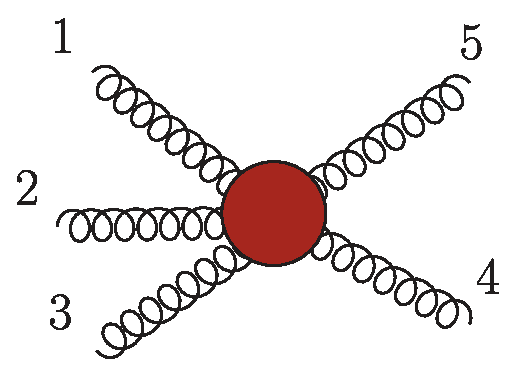
\includegraphics[height=\figureheight]{TreeFull}}} 
    \qquad \xrightarrow[p^2_\xi \to m_\xi^2]{} \quad
    \frac{1}{p^2_\xi - m_\xi^2} \cdot
    \sum_{i\in \text{states}}^{} ~
    \vcenter{\hbox{\includegraphics[height=0.9\figureheight]{TreeLeft}}}\cdot
    \vcenter{\hbox{\includegraphics[height=0.9\figureheight]{TreeRight}}}
  \end{equation*}
  \caption{
    An example of factorization due to a physical pole singularity. 
    Here $p_\xi =  p_1 + p_2 + p_3$.
  }
  \label{fig:factorization}
\end{figure}


\todo{Note that in \cref{eq:optical_theorem} there is a phase-space integral present on the right-hand side}

The exact singularity as expected cannot be reached in any physical process.
However if we analytically continue an amplitude to complex external momenta,
it is possible to choose them to hit the pole explicitly
while still satisfying on-shell conditions for external states.


\subsection{On-Shell Recursion}
\label{sec:BCFW}

The universal factorization  property expressed by \cref{eq:factorization_pole} is independent of perturbation theory. 
For tree-level amplitudes however the factorization can be discovered rather straightforwardly by inspection,
although it might be obscured in the expressions found within the standard Feynman-diagrammatic approach.

The factorization of tree amplitudes can be converted into an algorithm to evaluate them.
This is done through the systematic exploration of the amplitude's factorization limits such that
it can be broken down recursively to sums of lower-multiplicity tree amplitudes. 
The building blocks of this recursion are thus on-shell amplitudes.
This idea is known as \emph{Britto-Cachazo-Feng-Witten} (BCFW) recursion \cite{Britto2005c,Britto2005f}.
The on-shell recursion is a very powerful tool for analytical computations, especially 
in theories with supersymmetry \cite{Dixon:2010ik,Drummond:2008cr,Bourjaily:2010wh}.
However for numerical applications and general models the on-shell recursion algorithm
does not offer benefits over off-shell alternatives, both in speed and numerical stability \cite{Duhr:2006iq,Drummond:2008cr,Badger:2012uz},
especially if one is interested in tree amplitudes in arbitrary number of space-time dimensions (see \cref{chap:numunitarity}). 


\subsection{Generalized Cuts}

Unitarity can be turned into a computational method of loop amplitudes as well.
A certain class of one-loop amplitudes, which
can be written as a sum of box, triangle, and bubble scalar integrals,
\begin{equation} \label{eq:cut_constructable_ampl}
  A^{(1)} = \sum_i d_{i}\,\vcenter{\hbox{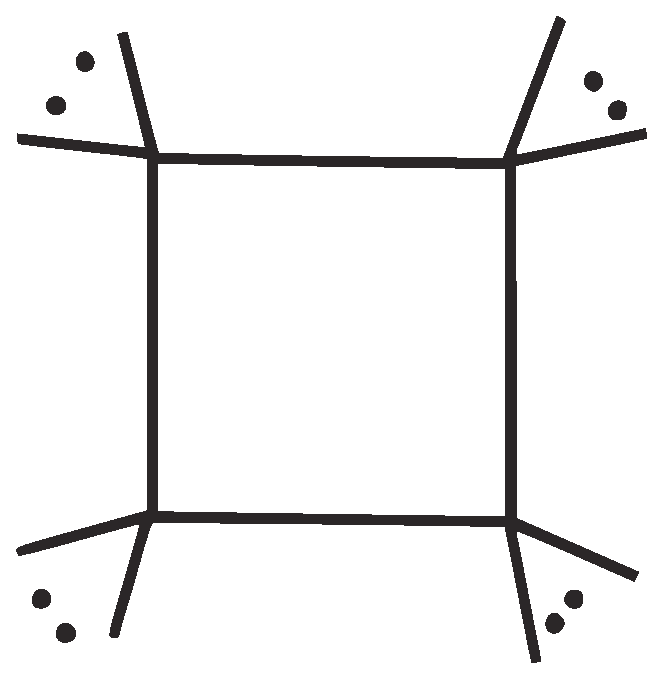
\includegraphics[width=8ex]{boxintegral}}}_i~+~
  \sum_{i}^{} c_{i}\,\vcenter{\hbox{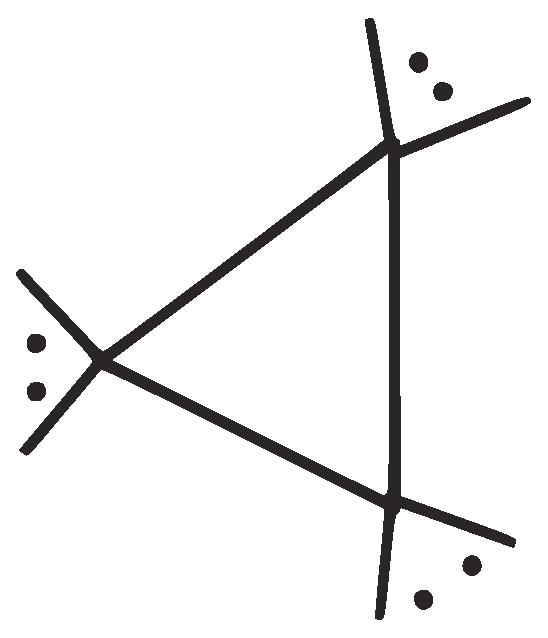
\includegraphics[width=7ex]{triangleint}}}_i~+~
  \sum_i b_{i}\,\vcenter{\hbox{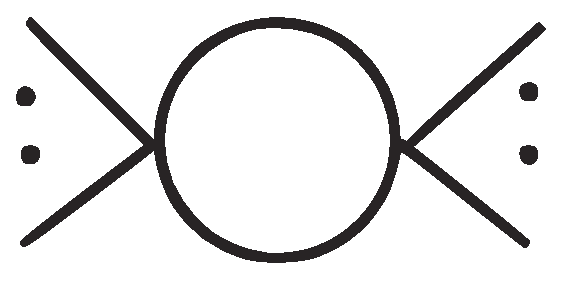
\includegraphics[width=8ex]{bubint}}}_i
\end{equation}
can be obtained entirely from unitarity cuts computed through Cutkosky rules \cite{Bern:1994cg,Bern:1994zx}.
Each integral in \cref{eq:cut_constructable_ampl} has unique discontinuities.
So the discontinuities of the loop amplitude on the left, 
evaluated as phase-space integrals over products of on-shell tree amplitudes as follows from unitarity,
can be matched to those of integrals to obtain equations for the integral coefficients.

However in general \emph{only} unitarity is not enough.

It is possible to generalize application of cuts given by \cref{eq:cut} to
obtain multi-channel discontinuities \cite{Britto:2004nc}.
For example see \cref{fig:quad_cut}.
Note that this kind of cuts are not direct consequences of unitarity of the $\mathcal{S}$-matrix (\cref{eq:unitarity_smatrix}), hence the name \emph{generalized} cuts.

\begin{figure}[ht]
  \centering
  \begin{equation*}
    \vcenter{\hbox{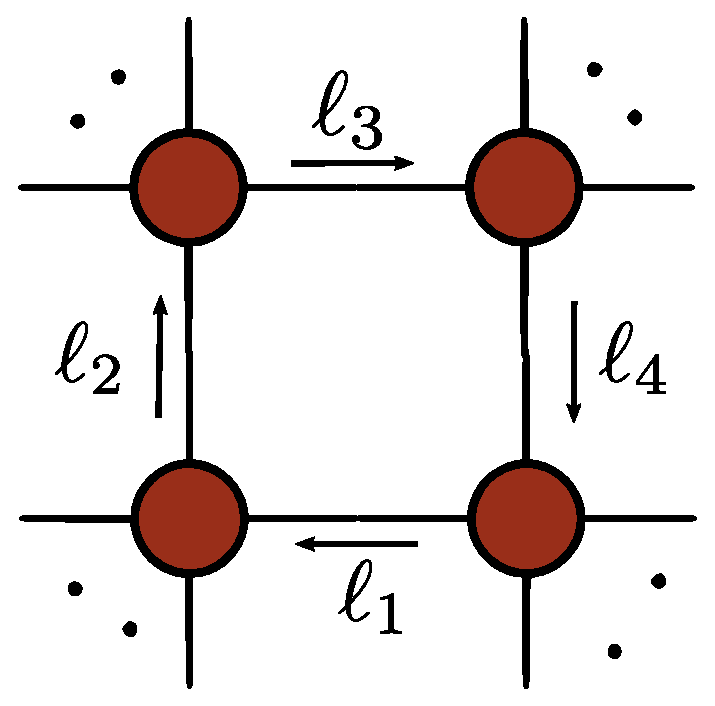
\includegraphics[width=0.2\linewidth]{box}}} \qquad \xrightarrow[i\in\{1\ldots4\}]{\ell_{i}^2-m_i^2\to~0} \qquad
    \vcenter{\hbox{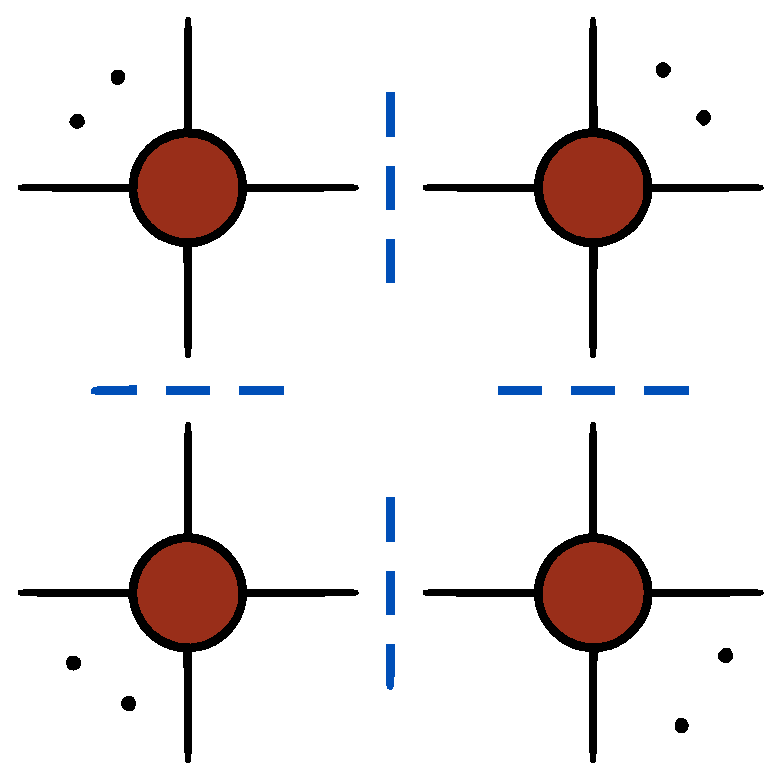
\includegraphics[width=0.2\linewidth]{boxCut}}}
    \quad = \quad \sum_{i}  c_{i} ~ m_{i}(\ell) %+ \sum_{i}  \tilde{c}_{i} \,\tilde{m}_{i}(\ell)
  \end{equation*}
  \caption{
    An example of a generalized cut.
    The loop momentum is chosen such that four propagator are simultaneously put to zero.
    On the left \emph{all} diagrams with the chosen propagators contribute.
    In the factorization limit each corner is a tree amplitude.
    The cut is matched to a basis of loop-momentum polynomials $\{m_i(\ell)\}$ on the right.
  }
  \label{fig:quad_cut}
\end{figure}


As a next step one can use the factorization of amplitudes on the cuts at the \emph{integrand} level  and match
it to a basis of loop-momentum polynomials in numerators (see \cref{fig:quad_cut}),
instead of integral coefficients \cite{Giele:2008ve,Ellis:2007br,Ellis:2008ir,Berger:2008sj}.
This matching procedure is intimately connected to a purely algebraical method of integral reduction known as OPP \cite{Ossola:2006us}.
This method uses the cut conditions \cref{eq:cut} to set some propagators to zero and triangularize linear systems for determining the basis coefficients.
It can be applied individually to each Feynman diagram or a sum thereof, thus having very little to do with factorization and unitarity.
When applied to the full amplitude however, it re

\todo{here unfinished} 
Somewhat confusingly sometimes generalized unitarity methods also refer 

Its flexibility allows for straightforward automation (see e.g.\ \cite{Berger:2008ag,Berger:2008sj,Cullen:2011ac,Mastrolia:2010nb,Ossola:2007ax}).

Most of the ideas mentioned in this section are formulated in the context of one-loop computations.
These give the first real taste of quantum nature of QFT.
Unfortunately, going beyond one-loop, many of the ideas do not generalize straightforwardly,
and require much more sophisticated computational techniques.
The extension of the ideas to multi-loop level have been actively studied in recent years \cite{Ita:2015tya,Abreu:2017idw,Abreu:2017hqn} 

In this thesis we apply the state-of-the-art developments for 


%%-------------------------------------------------

\chapter{Standard Techniques for Computation of Multi-Loop Amplitudes}
\label{chap:stdtech}
The aim of this chapter is to give a brief overview of standard computational methods for the
evaluation of multi-loop scattering amplitudes, and establish notation at the same time.

\section{Dimensional Regularization}



As we discussed in \cref{sec:hadcoll}, loop amplitudes exhibit UV and IR divergences,
which must cancel in computations of any observable quantity.
Thus, we regularize divergences in intermediate stages and leave the cancellations to the end. 
In principle, any consistent regularization prescription should suffice.
However, certain features of a regularization method such as breaking of Poincaré invariance or gauge symmetries
can impact dramatically its computational efficiency.
For this reason, many different regularization schemes have been studied (for a recent review see \cite{Gnendiger:2017pys}).

In this thesis, we regularize divergences by analytically continuing the dimensionality of space-time from four to $D = 4 - 2\eps$ dimensions.
Divergences manifest themselves in the limit $D\to4$ (or $\eps\to0$) as poles in $\eps$.
This idea is known as \emph{dimensional regularization} (DR) \cite{tHooft:1972tcz}.
Dimensional regularization has several advantages over other regularization schemes.
It explicitly preserves both Poincaré and non-chiral gauge symmetries.\footnote{Chiral gauge symmetries are in general violated by DR and require special treatment.}
Furthermore, it can be used as IR and UV regulator at the same time.
This makes it by far the most practical regularization scheme.


DR regularizes $L$-loop integrals by carrying out the integrations in $D$ dimensions, i.e.\ the integration measure is replaced as
\begin{equation}
  \int \prod_{i=1}^{L} \frac{\dd[4]{\ell_i}}{(2\pi)^{4}} ~\longrightarrow~ \quantity(\mu^{4-D})^{L}~\int \prod_{i=1}^{L} \frac{\dd[D]{\ell_i}}{(2\pi)^{D}},
  \label{eq:dimregmeasure}
\end{equation}
where $\mu$ is an arbitrary mass scale introduced to preserve the dimensionality of the coupling constants.
Accordingly the algebra of the kinematic variables is extended to $D$ dimensions, implying for instance
\begin{equation}
   \pdv{\ell^\mu_i}{\ell_{j\,\mu}} = \delta_{i j} D.
\end{equation}

The fields and states transform as representations of Poincaré group,
implying that all Lorentz tensor and spinor structures (such as the metric tensor, momenta, external states, etc.\@) have
to be generalized to $D$ dimensions.
There are different flavors of DR making particular choices on how this generalization is accomplished (see e.g.\ \cite{Gnendiger:2017pys}).

The conceptually simplest variant of DR, the \emph{conventional dimensional regularization} (CDR)
treats all Lorentz structures uniformly in $D$ dimensions, effectively replacing the $\mathrm{SO}(1,3)$ Lorentz symmetry by $\mathrm{SO}(1,D-1)$.
CDR has been successfully employed in many analytic computations.
In this thesis, however, we are concerned with numerical methods, for which CDR is not practical due to
(formally infinite) number of additional external states.
Instead, we use the 't Hooft -- Veltman (HV) scheme which keeps all external states and momenta in four dimensions.
%and extends the space-time symmetry group to $\mathrm{SO}(1,3)\otimes \mathrm{SO}(D-4)$.

It is advantageous to distinguish in the intermediate stages of computation the dimensionality of loop integration (or loop momenta) $D$ and
the dimensionality of internal particles $D_s \geq  D$.
We will extensively exploit this separation in \cref{chap:dshel} to derive an efficient numerical algorithm
for the evaluation of amplitudes in the HV scheme.


\section{Loop Amplitudes}

For a particular choice of a gauge group, particle content, and operators of
a theory (which we collectively call a \emph{model}), Feynman rules can be derived.
Then the amplitudes in \cref{eq:amplitudes_expansion} can be obtained as a sum of all Feynman diagrams
with $N = 2+n$ specified external particles and $L$ loops.
For the purpose of this chapter, we assume that the amplitudes $A^{L}_N$ are Lorentz-scalars.
This can be achieved for example through decomposition into form factors (see \cref{chap:dshel}),
and details of this procedure are of no importance here.

The most general form for any $L$-loop amplitude with $N$ external particles with momenta $p_1,\ldots,p_N$ is
\begin{equation}
  \sum_{\Gamma \in \Delta} \sum_{\gamma_\Gamma} \qty(\int \prod_{l=1}^{L} \tilde{\dd{\ell_l}}) ~ 
  \frac{\mathcal{N}_{\Gamma,\gamma_\Gamma}%(\ell_1,\ldots,\ell_L,p_1,\ldots,p_{N-1})
    }{\prod_{j\in P_\Gamma} \rho_j^{\gamma_{\Gamma j}}},
    \qquad \tilde{\dd{\ell_l}} \coloneqq \frac{\dd[D]{\ell_l}}{(2\pi)^{D}}.
  \label{eq:general_amplitude}
\end{equation}
Here, $\rho_j = q_j^2 - m_j^2$ is a denominator of a propagator with momentum $q_j$ and mass $m_j$. The sum $\sum_{\gamma_\Gamma}$ runs through all assignments
of exponents $\gamma_{\Gamma j} > 0$ of each propagator $\rho_j$. 
A \emph{topology} $\Gamma$ is identified with a particular set of (unique) propagators $P_\Gamma$,
treating two sets of propagators equal if one can be transformed into the other with linear re-parametrizations of loop momenta.
Note that topologies defined in this sense might have multiple graph representations.
The external sum runs over a set of all distinct topologies $\Delta$ contributing to the amplitude.
The numerators $\mathcal{N}_{\Gamma,\gamma_\Gamma}$
are functions of all possible scalar products of loop momenta, external momenta and polarization states.

Carrying out loop integrations in \cref{eq:general_amplitude} is a challenging task in general.
Fortunately, there are many relations between integrals in \cref{eq:general_amplitude},
and it is thus sufficient to consider a significantly smaller set of integrals $\Delta_M \subset \Delta$, commonly referred to
as \emph{master integrals}.
Taking the integral relations into account the amplitude can be written in the form
\begin{equation}
  \sum_{\Gamma \in \Delta_M} \sum_{i\in M_\Gamma} ~ c_{\Gamma,i} ~ I_{\Gamma,i}, 
    \qquad I_{\Gamma,i} \coloneqq 
      \qty(\int \prod_{l=1}^{L} \tilde{\dd{\ell_l}}) \frac{m_{\Gamma,i}}{\prod_{j\in P_\Gamma} \rho_j^{\gamma_{\Gamma i,j}}},
  \label{eq:amplitude_integrated}
\end{equation}
where $M_{\Gamma}$ is a set of numerator insertions $m_{\Gamma,i}$ and exponents $\gamma_{\Gamma i}$.
Despite the fact that the numerator functions $\mathcal{N}_{\Gamma,\gamma_\Gamma}$ in \cref{eq:general_amplitude} depend on the types of external particles and a particular model,
the master integrals $I_{\Gamma,i}$ are universal and determined only by kinematics.

Evaluation of amplitudes can thus be separated into two different problems:
\begin{enumerate}
  \item Extracting  the list of all relevant topologies and numerator insertions from \cref{eq:general_amplitude},
    identifying the master integrals and computing them.
  \item Reducing all terms in \cref{eq:general_amplitude} to the form of \cref{eq:amplitude_integrated}, thus
    determining the coefficients $c_{\Gamma,i}$.
\end{enumerate}
The process- and model-dependent information is contained in the master-integral coefficients $c_{\Gamma,i}$,
so the master integrals can be recycled for all kinematically-equivalent amplitudes.

In this thesis, we focus on the reduction to master-integral coefficients.
We will review the standard approach in the next section, and
then explain how unitarity-based methods allow us to address some of its difficulties in \cref{chap:numunitarity}.

\section{Classification of Numerators}
\label{sec:classification_numerators}

To carry out the task of reduction,
we need to classify all possible structures that can appear in the numerator functions $\mathcal{N}_{\Gamma,\gamma_\Gamma}$ in \cref{eq:general_amplitude}.

We start by making a convenient choice of independent variables.
Due to Lorentz-invariance, the numerators $\mathcal{N}_{\Gamma,\gamma_\Gamma}$ can only depend on scalar products
\begin{equation}
  \label{eq:sps_all}
  \vb*{sp} = \{ \sp(\ell_i,\ell_j),~\sp(\ell_i,p_j),~\sp(\ell_i, \tau_j) \}, \qquad \dim{\vb*{sp}} = D_{\text{ext}} L + \frac{1}{2}L(L+1),
\end{equation}
where $D_{\text{ext}}$ is the dimensionality of external states and momenta.
Here the vectors $\tau_i$ are the basis of the orthogonal complement of $\spn{p_1,\cdots,p_{N-1}}$ to the full four-dimensional Minkowski space,
so we have $p_i \cdot \tau_j = 0$ and $\tau_i \cdot \tau_j = \delta_{ij}$.
The directions $\tau_i$ can be introduced into $\mathcal{N}_{\Gamma,\gamma_\Gamma}$ through external polarization states, hence,
the scalar products $\sp(\ell_i, \tau_j)$ will drop out if polarization sums are performed.
In the HV scheme, $D_{\text{ext}}=4$ and the number of corresponding scalar products are
\begin{equation}
  \label{eq:sp_counts}
  \renewcommand{\arraystretch}{1.5}
  \begin{tabular}[h]{p{10ex} p{20ex}}
    %$3N-10$ & $\sp(p_i,p_j)$ \\
       $\sp(\ell_i,\ell_j)$  &   $\dfrac{1}{2}L(L+1)$                \\
        $\sp(\ell_i,p_j)$    &   $\min\qty(4,N-1) ~L$                  \\
       $\sp(\ell_i, \tau_j)$ &   $ \qty\big(4-\min\qty(4,N-1)) L $  \\
  \end{tabular}
\end{equation}

The numerators $\mathcal{N}_{\Gamma,\gamma_\Gamma}$ can be thus represented as elements of a polynomial ring
$\mathbb{Q}_{\vb*{x},D}[\vb*{sp}]$ 
with coefficients $c_{\va{i}}(\vb*{x},D)$ take values int the field of rational functions $\mathbb{Q}_{\vb*{x},D}$ of external kinematics $\vb*{x}$
and $D$:~\footnote{
  $\vb*{x}$ is understood to be a list of variables corresponding to some parametrization of external kinematics, which we will not need to specify explicitly here.
}
\begin{equation}
  \mathcal{N}_{\Gamma,\gamma_\Gamma}(\vb*{x}, \vb*{sp}, D) = \sum_{\va{i} : \abs{\va{i}} < H_{\Gamma}} c_{\va{i}} (\vb*{x},D)~ m^{\va{i}}(\vb*{sp}),
  %m^{\va{i}}(\vb*{sp}) = (\sp(\ell_1,\ell_1))^{i_1} ~\cdots~ (\sp(\ell_1,p_1))^{i_{\min\qty(4,N-1)L}} ~\cdots~,
  \qquad m^{\va{i}}(\vb*{sp}) = \mathrm{sp}_1^{i_1} ~\ldots{}~ \mathrm{sp}_{\dim{\vb*{sp}}}^{i_{\dim{\vb*{sp}}}},
  %%(\sp(\ell_L, \tau_{4-\min\qty(4,N-1)}))^{\i_{\dim{\vb*{sp}}}}
\end{equation}
where the sum runs over all monomials $m^{\va{i}}(\vb*{sp})$ with \emph{total degree} $\abs{\va{i}} \equiv \sum_j i_j$ less than
some maximal value $ H_{\Gamma} $ determined by the UV structure of the model in consideration.


For a given topology $\Gamma$ in \cref{eq:general_amplitude} we chose $N_p$ denominators $\vb*{\rho}\coloneqq\{\rho_1,\ldots,\rho_{N_p}\} \in P_\Gamma$ as
independent variables. Then $N_p$ scalar products from the set $\vb*{sp}$
can be expressed as linear functions of denominators $\vb*{\rho}$.
This implies that whenever these scalar products are encountered in $\mathcal{N}_{\Gamma,\gamma_\Gamma}\qty(\vb*{sp})$,
they can be canceled with one of the denominators and attributed to a topology with fewer propagators,
leaving only a scalar remainder (i.e.\ independent of loop-momenta) in the numerator of $\Gamma$.
For this reason, these scalar products are commonly called \emph{reducible scalar products} (RSP).
We choose the remaining scalar products
\begin{equation}
  \vb*{\alpha} \coloneqq \vb*{sp} \setminus \{\text{RSPs}\} , \qquad N_\text{ISP} \coloneqq \dim{\vb*{\alpha}}   =  \dim{\vb*{sp}}-N_p,
\end{equation}
which are called
\emph{irreducible scalar products} (ISP) to be the remaining independent variables.

An important observation which becomes evident from our choice of variables is that all topologies with $N_p> 4 L +\frac{1}{2}L(L+1)$ are reducible.
Indeed, in this case we have $\dim\vb*{sp} < N_p$ so there are no irreducible scalar products, and only $(\dim\vb*{sp})$ denominators can be independent.

After a change of variables $\vb*{sp}\to \{\vb*{\rho},\vb*{\alpha}\}$ and cancellation of denominators
we find that the numerators are now polynomials in ISPs only:
\begin{equation} \label{eq:rsp_reduction}
  \mathcal{N}_{\Gamma,\gamma_\Gamma}(\vb*{x}, \vb*{sp}, D) \longrightarrow \qquad
    \mathcal{N}^{\prime}_{\Gamma,\gamma_\Gamma}(\vb*{x}, \vb*{\alpha}, D) =
    \sum_{\va{i} : \abs{\va{i}} < H_{\Gamma}} c^{\prime}_{\va{i}} (\vb*{x},D)~ m^{\va{i}}(\vb*{\alpha}),
\end{equation}
and all topologies with $N_p > 4L +\frac{1}{2}L(L+1)$ are eliminated.
In practice, this can be non-trivial and systematically performed with Gröbner basis techniques \cite{Zhang:2012ce,Mastrolia:2012wf,Mastrolia:2012an,Mastrolia:2016dhn}.
In unitarity-based approaches, this step is taken into account by construction,
and need not be carried out explicitly. We discuss this in more detail in \cref{sec:ansatz_integrand}

For $L=1$, the only irreducible scalar products are of the transverse type $\sp(\ell_i, \tau_j)$, which vanish upon integration due to Lorentz symmetry either directly,
or after some simple considerations (see \cref{sec:traceless_completion} for details).
For $L>1$, however, this is not the case and there are more identities that we can take advantage of to reduce the number of master integrals.
We discuss this in the next section.

We conclude this section with a remark that the variables $\{\vb*{\rho},\vb*{\alpha}\}$ we chose for parametrization of the integrand can be promoted
to the integration measure in \cref{eq:general_amplitude}. This representation of loop integrals known as the \emph{Baikov representation} \cite{Baikov:1996rk} 
makes $4 L +\frac{1}{2}L(L+1)$  non-trivial integrations manifest and allows to trivially integrate out irrelevant loop-momenta directions. This representation
exhibits many other useful properties, nonetheless, we will not need to adopt it in this thesis.


%We parametrize loop momenta as follows
%\begin{subequations}
  %\begin{equation}
    %\ell_l = \ell_{l[4]} + \ell_{l[D-4]}, \qquad 
    %\begin{array}[]{ll}
      %\ell^\mu_{l[4]} &\coloneqq g^{\mu\nu}_{[4]} \ell_\nu \\
      %\ell^\mu_{l[D-4]} &\coloneqq g^{\mu\nu}_{[D-4]} \ell_\nu \\
    %\end{array},
    %\qquad
    %\ell_{l[4]}\cdot\ell_{l[D-4]} = 0,
    %\label{eq:loop_momenta}
  %\end{equation}
  %and
  %\begin{align}
    %\ell_{l[4]} &=  \sum_{i\in \mathcal{B}_{\text{phys}}} c^{i}_l ~ v^{i} ~+~ \sum_{i\in \mathcal{M}_{[4]}\setminus\mathcal{B}_{\text{phys}}} \chi^{i}_l ~ \tau^i, \\ 
    %\ell_{l[D-4]} &=  \sum_{i\in\tilde{\mathcal{B}}} \mu^i_l ~ \tilde{n}^{i},
  %\end{align}
%\end{subequations}
%where $v^{i}$ are basis vectors of the vector space $\mathcal{B}_{\text{phys}} \coloneqq \spn{p_1,\cdots,p_{N-1}}$ spanned by $N-1$ external momenta;
%the vectors $\tau_i$ span the orthogonal complement of $\mathcal{B}_{\text{phys}}$ to the four-dimensional Minkowski space $\mathcal{M}_{[4]}$.


\section{Integration-by-Parts Identities}
\label{sec:ibp}


Using \cref{eq:rsp_reduction} we can bring \cref{eq:general_amplitude} to the form 
\begin{equation} \label{eq:rsp_reduced_amplitude}
  \sum_{\Gamma \in \Delta} \sum_{\gamma_\Gamma} \sum_{\va{i}} ~ c_{\Gamma\gamma_\Gamma, \va{i}} (\vb*{x},D) ~ 
  \qty(\int \prod_{l=1}^{L} \tilde{\dd{\ell_l}}) ~  
  \frac{m^{\va{i}}(\vb*{\alpha})%(\ell_1,\ldots,\ell_L,p_1,\ldots,p_{N-1})
    }{\prod_{j\in P_\Gamma} \rho_j^{\gamma_{\Gamma j}}}.
\end{equation}
The integrals in \cref{eq:rsp_reduced_amplitude} are process-independent and have the desired form of \cref{eq:amplitude_integrated}.
However, we are still missing a large number of identities, which are present due to the vanishing of the total derivative in dimensional regularization.
These identities are known as \emph{integration-by-parts} (IBP) identities \cite{Chetyrkin:1981qh,Tkachov:1981wb} and have a general
form of
\begin{equation}
  \qty(\int \prod_{l=1}^{L} \tilde{\dd{\ell_l}}) ~  \pdv{\ell_k^\mu}(
  \frac{ v_k^\mu \ommit{(\vb*{x},\vb*{\rho},\vb*{\alpha},D)} ~ \, m^{\va{i}}(\vb*{\alpha})
    }{\prod_{j} \rho_j^{\gamma_{j}}}
    ) = 0,
  \label{eq:ibps}
\end{equation}
where the components of \emph{IBP vectors} $v_k^\mu(\vb*{x},\vb*{\rho},\vb*{\alpha},D)$ are arbitrary rational functions
of all variables. The monomials $m^{\va{i}}(\vb*{\alpha})$ can be absorbed in $v_k^\mu$, but
it is convenient to keep them separate.

It is useful to organize all topologies $\Delta$ in \cref{eq:rsp_reduced_amplitude}
hierarchically by defining a partial ordering
\begin{equation} \label{eq:topology_order}
    \Gamma_1 > \Gamma_2 \iff P_{\Gamma_1} \supset P_{\Gamma_2},
\end{equation}
meaning that topology $\Gamma_2$ is obtained from topology $\Gamma_1$ by removing one or more propagators.
We then slice $\Delta$ into strictly ordered (overlapping) subsets $\Delta_i$ such that
\begin{subequations} \label{eq:topology_sequence}
    \begin{gather}
         \Delta = \bigcup_i \Delta_i,  \\
         \Delta_i  = \{\Gamma \in \Delta : \forall \, \Gamma_1, \Gamma_2 \in\Delta \qif\qty( \Gamma_1 \in \Delta_i \qand \Gamma_2 < \Gamma_1) \qthen \Gamma_2 \in \Delta_i \}.
    \end{gather}
\end{subequations}
A subset $\Delta_i$ can thus be identified by its ``greatest'' topology $\Gamma_{\Delta_i}$ ---
the topology with the maximal number of propagators, which we will call a \emph{parent} topology (or diagram).

If we allow exponents $\gamma_{\Gamma j}$ in \cref{eq:rsp_reduced_amplitude} to also be $\leq0$,
all integrals in \cref{eq:rsp_reduced_amplitude} can be cast into \emph{families}
\begin{equation} \label{eq:integral_families}
    I_{\Delta_i}[\va{\gamma},\va{i}] \coloneqq 
  \qty(\int \prod_{l=1}^{L} \tilde{\dd{\ell_l}}) ~  
  \frac{m^{\va{i}}_{\Gamma_{\Delta_i}}(\vb*{\alpha})%(\ell_1,\ldots,\ell_L,p_1,\ldots,p_{N-1})
    }{\prod_{j\in P_{\Gamma_{\Delta_i}}} \rho_j^{\gamma_{j}}}.
\end{equation}
IBP identities of \cref{eq:ibps} generate an under-determined system of homogeneous linear equations between integrals inside a family.\footnote{
  In some exceptional cases IBP identities can relate integrals between different families, but we will not need to consider them in this thesis. 
}
The integrals which cannot be determined from the system are chosen to be master integrals.
The remaining integrals are then expressed as linear combinations of master integrals.
A systematic approach of generating and solving a complete system of IBP identities was formulated by Laporta \cite{Laporta:2001dd}.
There are multiple publicly-available implementations such as
\textsc{Reduze} \cite{Studerus:2009ye,vonManteuffel:2012np},
\textsc{Fire} \cite{Smirnov:2008iw,Smirnov:2014hma},
\textsc{LiteRed} \cite{Lee:2012cn,Lee:2013mka},
\textsc{Kira} \cite{Maierhoefer:2017hyi,Maierhofer:2018gpa}, etc.

The task of IBP reduction is in general very difficult.
This is due to a large number of relations produced by \cref{eq:ibps},
which is in turn due to the number of choices of IBP vectors, as well as the fact that IBP identities,
in general, include the relations for integrals with raised denominator powers, even
though these integrals are mostly not found from Feynman rules.
In the end, the bottleneck is coming from the requirement to solve large systems of linear equations.
Many great improvements to the IBP-reduction technology have been suggested
\cite{Gluza:2010ws,Schabinger:2011dz,Larsen:2015ped,Bern:2017gdk,Chawdhry:2018awn,Kosower:2018obg,Mastrolia:2018uzb,Frellesvig:2019kgj,Frellesvig:2019uqt,Bendle2019}
since the Laporta algorithm became widespread.
It was also proposed to reconstruct the reduction tables from
numerical evaluations over finite fields \cite{vonManteuffel:2014ixa,Peraro:2016wsq,Peraro:2019svx,Klappert:2019emp,Smirnov:2019qkx}.
However, there is still a problem
that even when the analytic reduction tables can be obtained,
it might be challenging to use them for the reduction of amplitudes due
to the prohibitive size of expressions (see e.g.\ \cite{Chawdhry:2018awn,Bendle2019}).
Because of these complications it seems beneficial to carry out IBP reduction numerically and reconstruct
analytic expressions for amplitudes instead \cite{Badger:2018enw,Chicherin:2018yne,Badger:2019djh}.

In this thesis, we will take advantage of generalized unitarity-based methods (see \cref{chap:numunitarity}),
which do not require solving IBP systems and thus,
avoid some of the problems discussed above.

\section{Master Integrals}

Once the set of master integrals is found, the IBP reduction relations can be applied 
to all terms in \cref{eq:rsp_reduced_amplitude}.
This determines the coefficients of master integrals
\begin{equation} \label{eq:master_integrals}
    \qquad I_{\Gamma,i} = 
    \qty(\int \prod_{i=1}^{L} \tilde{\dd{\ell_i}}) \frac{m_{\Gamma,i}}{\prod_{j\in P_\Gamma} \rho_j^{\gamma_{\Gamma i,j}}}.
\end{equation}
in \cref{eq:amplitude_integrated}.

A variety of methods have been developed for the evaluation of the master integrals.
Broadly speaking, they can be classified into analytic and numerical methods.

Direct integration using a convenient choice of integration variables is the most straightforward option.
Most one-loop integrals have been obtained this way \cite{vanHameren:2010cp,Ellis:2007qk,tHooft:1978jhc,Denner:2010tr}.
However, for multi-scale multi-loop integrals this becomes  cumbersome   very quickly.
Another method is the integration in the Mellin-Barnes  representation  \cite{Smirnov:1999gc,Tausk:1999vh,Dubovyk:2017cqw}, which
has been used to solve some two-loop integrals.
However, the most commonly used and successful method is to obtain analytic results via
differential equations \cite{Kotikov:1990kg,Remiddi:1997ny,Gehrmann:1999as,Henn:2013pwa,Argeri:2007up,Henn:2014qga}
brought into their canonical form \cite{Henn:2013pwa}.
These equations are obtained by noticing that
derivatives of master integrals with respect to
external invariants or masses can be IBP-reduced to the linear vector space of master integrals from the same family.
Thus the whole family of integrals can be obtained from solving the system of linear differential equations.

On the numerical side (see e.g.\ \cite{Freitas:2016sty} for a comprehensive review),
the commonly used general methods are sector decomposition \cite{Binoth:2000ps,Binoth:2003ak}
and numerical integration in Mellin-Barnes representation \cite{Czakon:2005rk,Anastasiou:2005cb}.
Usually, the knowledge of analytical expressions is preferable since it allows for better control over
precision and performance required for Monte-Carlo integration over external phase space. However,
some notable NNLO QCD computations have been carried out with at least one of the integrals evaluated through numerical
methods \cite{Jones:2018hbb,Grazzini:2018bsd,Baglio:2018lrj}.

There are no constraints on the choice of basis of master integrals, apart from the linear-independence under IBP relations. 
This freedom can be exploited to facilitate particular aspects of the computation.
The basis of uniformly transcendental (UT) or pure integrals \cite{ArkaniHamed:2010gh} has a simple form of the
associated differential equations \cite{Henn:2013pwa}, which allows to solve them in terms of iterated integrals.
For numerical evaluations, as well as for exploring the structure of divergences of amplitudes,
it is often beneficial to make master integrals finite by constructing the so-called local integrands \cite{ArkaniHamed:2010kv,ArkaniHamed:2010gh,Badger:2016ozq,Badger:2016egz}.
Another numerically-oriented choice is the quasi-finite basis \cite{vonManteuffel:2014qoa,Panzer:2014gra}.
Finally, in the numerical unitarity method, which we discuss in \cref{chap:numunitarity}, the master integrands are required to have no doubled propagators.
The conversion between different master-integral bases is often simpler than obtaining the relations for high-degree numerator insertions,
and can be performed with the standard IBP reduction techniques.

In this thesis, we will not consider the evaluation of master integrals.
For the class of process we are interested in, the analytic results are available in the literature \cite{Gehrmann:2018yef,Papadopoulos:2015jft,Gehrmann:2000zt}.


\chapter{Multi-Loop \texorpdfstring{$D$}{D}-Dimensional Numerical Unitarity}
\label{chap:numunitarity}
In this chapter we introduce the main computational methods we used to obtain results of
\cref{chap:wbb_pheno,chap:5parton}. 

We will describe a complete generalization of unitarity techniques to multi-loop level.

With aim for automation and fully numerical.

Some partial attempts can be found in 


In this chapter we do not refer to a particular theory.


Based on the papers

I want to take the pragmatic perspective. And in practice it is not even essential:
\begin{itemize}
    \item       the most practical and flexible way to compute them in $D$ dimensions is with off-shell recursions (see references e.g. in tails of 1001 gluons)
    \item Actually it is not even always the case as we see for massive particles.
\end{itemize}

LHS can be just an expression obtained from Feynman diagrams

However in perturbation theory the fact that the corners are tree amplitudes can be seen explicitly.
Because we collect together all graphs containing a particular singularity.


\section{Ansatz}
\label{sec:ansatz_integrand}

\subsection{Basis of Numerator Insertions}
Numerator tensors, span of function space. Master/Surface decomposition.

\todo{classification of tensors here or in chapter \ref{chap:stdtech}?}




\subsection{Traceless Completion}
\label{sec:traceless_completion}

Starting from two loops will have $D$-dependence in the numerator from IBP identities, so
we can choose to abandon all-together the idea of not having it there.

Also can be obtained with through a specially constructed IBP identities \cite{Ita:2015tya}.
%vectors of the form 
%\begin{equation}
  %v^\mu = (\sp(n_\epsilon^i,\ell))~\ell^\mu - (\sp(\tau,\ell))~n_\epsilon^{i\,\mu}
%\end{equation}


\subsection{Unitarity-Compatible IBP Identities}

\section{Cut Equations}

\subsection{On-Shell Loop-Momenta}

\todo{In $D$ dimensions we don't have to worry about branches of solutions, and also loop momenta have to be real}

\subsection{Evaluation of Cuts}

\subsection{Off-Shell Recurcion}
\label{sec:BG_recursion}

$D$-dimensional off-shell recursion, 


weyl and Dirac fermions, 
tracking of representations?


\subsection{Dimensional Reconstruction}
 In $D$ and $D_s$ (dimensional reduction later)


\section{Subleading Poles}
Here discussion about \textit{subleading poles}



\section{Examples}

\subsection{One-Loop Hierarchy}

Once the automated approach is set up, the one-loop case is so simple that we can
do the full one-loop hierarchy.

Compare to ``normal'' decomposition, we allow $D$-dependence in numerators. This might be not the best
idea for NLO computations since terms of order $\mathcal{O}(\epsilon)$ can be dropped.
It might be reasonable to do for higher-order computations where higher orders of $\epsilon$ are required.


Take 5-point hierarchy.

\subsubsection{Pentagon}

Take $\mu^2$ insertion.

\subsubsection{Box}

\subsubsection{Triangle}

Here also show that 1 and 2 mass triangles can be reduced

\subsubsection{Bubble}

See what happens with the light-like external momentum from the IBP perspective?
Should work out.

\subsubsection{Tadpole}

\subsection{Some Two-Loop Topology}

\todo{select a topology which is not too big to present} 




%-------------------------------------------------

\chapter{Dimensional Regularization and Helicity Amplitudes
%in a Numerical Framework
}
\label{chap:dshel}
The full physical information about a process is contained in a complete set of \textit{helicity amplitudes}.

They are calculated by selecting all external states of particles to be the states with definite helicity \todo{define what helicity is}.

It is well known that helicity amplitudes exhibit nice physical properties such as trivialization of gauge-invariance and
manifestation of Poincare symmetry \todo{some references}.

From a technical perspective this means that helicity amplitudes are ``good'' objects to compute. \todo{this is very rough formulation}

As we mentioned before, amplitudes with loops exhibit divergences, which forces us
to use dimensional regularization.\footnote{other regularization methods exist \todo{reference}, but this is out of the scope of this thesis}


Formally then the corresponding space is infinite-dimensional \todo{reference Collins}, and
it can be made to ``coincide'' with the finite-dimensional one whenever $D$ takes integer values.

In CDR we replace $SO(1,3)$ invariance by $SO(1,D-1)$.
In HV by $SO(1,3)\otimes SO(D-4)$.

After all divergences are cancelled, the limit $D\to4$ is taken and the physical results are recovered.

All particle transform as irreducible representations of Poincare group in $D$ dimensions,
so the number of states becomes infinite.
This raises the question as to how to define a helicity amplitude in the framework of dimensional regularization.


\section{Tensor Decomposition and Projectors}

In this section we review a way to define helicity amplitudes in dimensional regularization through
$D$-dimensional projectors.

This approach has been used in a number of computations \cite{Garland:2002ak, Moch:2002hm, Glover:2003cm, Glover:2004si,Gehrmann:2009vu,Gehrmann:2011aa}.
It's relation to HV scheme and helicity amplitudes has been recently further clarified \cite{Peraro:2019cjj}.

One starts with decomposing an amplitude with unspecified external states into all possible $D$-dimensional tensor structures compatible
with symmetries. One finds a basis of these structures and finds corresponding $D$-dimensional projectors.
At this point the calculation is done in CDR using $D$-dimensional tensor and Clifford algebras.

Then one switches to the HV scheme by decomposing projectors in $4$ and $(D-4)$ parts,
and chooses four-dimensional helicity states as a basis.
And helicity amplitudes are found by constructing appropriate linear combinations of projectors.
Some of the initial coefficients become irrelevant.

The complexity and number of initial projectors grows very fast with the number of external particles, as was demonstrated in \cite{Peraro:2019cjj}.

Projection approach is a backwards way of doing helicity amplitudes.

Note that asking for helicity amplitudes makes sense only in HV scheme.


\section{HV Helicity Amplitudes from Embedding of States}

We show how to obtain helicity amplitudes directly, without complicated projectors,
for vector and spinor particles.
We achieve this by working in HV scheme from the get-go, and by
choosing an appropriate embedding of the physical four-dimensional state in $D$ dimensions.

This is trivially achieved for gluon helicity states: these
are vector particles and any four-dimensional polarization state
can be embedded in a generic $D$-dimensional space by filling 
the remaining components of the vector with zeros. 
For fermion states, however, the embedding is less trivial as 
the nature of the $D$-dimensional Clifford algebra means that
there is no single associated state in $D$-dimensions.  

As such, one might wonder if it is possible at all to unambiguously 
define four-dimensional helicity amplitudes with external
fermions. In this section we describe how we
address this problem, inspired by the approach of
refs.~\cite{Glover:2003cm,Glover:2004si}.
 
This generalizes the prescription of EGKM for one-loop to multi-loop and
multi-quark (also massive).

\subsection{Embedding of Vector States}

\subsection{Embedding of Spinor States}
\label{sec:Clifford}


There are several consistent regularization schemes that can be
chosen, see
e.g.\ ref.~\cite{Gnendiger:2017pys} for a recent review, and our
discussion applies to both the conventional
dimensional regularization (CDR) and the 't Hooft-Veltman (HV)
schemes. The two schemes differ in the way
vector particles (gluons in our case) are treated,
and we follow 
the description given in the reference
above.\footnote{Except for the meaning of $D_s$, which we use 
to denote the dimension of the CDR and HV singular vector 
fields, to differentiate it from the dimensional regulator $D$.}
In CDR, all vector fields are vectors in a space of dimension
$D_s=4-2\epsilon$. In
HV, one distinguishes between \emph{regular} and 
\emph{singular} vector 
fields. The former do not lead to any singularities and 
are considered to be
strictly four-dimensional objects. The
latter are a source of singularities and are 
$D_s$-dimensional vectors. For our purposes, this means
that gluons whose momentum we integrate over are 
$D_s$ dimensional, and external gluons whose momentum
we do not integrate over are
four dimensional. The two schemes are consistent,
in that their contributions to NNLO computations can be related by known
transition rules~\cite{Broggio:2015dga}, but as we
shall see below the HV scheme introduces some simplification in
the calculation.


We consider fermions in $D_s$ dimensions, as is for instance
necessary when a CDR gluon or a singular HV gluon is emitted 
from a quark line. If the fermion line closes upon itself, as in
e.g.\ the $N_f$ corrections to gluon amplitudes
(i.e.\  corrections with a closed massless-quark loop), 
we only need the defining
property of the Clifford algebra
\begin{equation} \label{eqn:defClifford}
\{ \gamma_{[D_s]}^\mu, \gamma_{[D_s]}^\nu \} = 
2 g_{[D_s]}^{\mu\nu}\mathbb{1}_{[D_s]}^{\vphantom{\mu\nu}} \,,
\end{equation}
where we explicitly write the dimension $D_s$
as a subscript of the $\gamma$-matrices and the metric, and
use a metric with mostly-minus Minkowski signature, 
$g_{[D_s]}=\mathrm{diag}\{1, -1 , ... , -1 \}$.
Here $\mathbb{1}_{[D_s]}$ is the identity operator in the representation space of 
the Clifford algebra.
In the presence of external fermions, however, 
we must also describe the corresponding states and
an explicit
representation of the $D_s$-dimensional Clifford algebra is
required. Since we are ultimately interested in specifying
four-dimensional
external states, it is furthermore convenient to construct 
the representation in a factorized way starting from four dimensions
(see e.g.\ refs.~\cite{Kreuzer:susylectures,Collins:1984xc}).
We thus consider a Clifford algebra
in $D_s$ dimensions as the tensor product of a
four-dimensional and a $(D_s-4)$-dimensional one:
\begin{equation}\label{eqn:cliffordrecursion}
%
(\gamma_{[D_s]}^\mu)_{a\kappa}^{\,b\lambda}  = \left\{ 
\begin{array}{ll} 
		\left(\gamma_{[4]}^\mu\right)_a^{\;b} \,
		\delta_\kappa^\lambda\,, &\quad  0\le\mu \le 3 \,,\\&\\
		\left(\tilde\gamma_{[4]}\right)_a^{\;b} 
		\left(\gamma_{[D_s-4]}^{(\mu-4)}\right)_\kappa^{\;\lambda}\,, 
        &\quad \mu > 3 \,,
\end{array}
		\right.
%
\end{equation}
where $\tilde\gamma_{[4]}\equiv i(\gamma_{[4]}^0
\gamma_{[4]}^1 \gamma_{[4]}^2 \gamma_{[4]}^3)$, such that 
$(\tilde\gamma_{[4]})^2 =\mathbb{1}_{[4]}$ is the identity
operator
in the four-dimensional algebra.
The indices $a,b$ denote the spinor indices in the
four-dimensional algebra and $\kappa,\lambda$ the ones of the 
$(D_s-4)$-dimensional one.
The $\gamma^\mu_{[D_s-4]}$ form themselves a 
$(D_s-4)$-dimensional Clifford algebra with signature
$g_{[D_s-4]}=\mathrm{diag}\{ -1 , ... , -1 \}$.
In amplitude calculations we naturally encounter products of
$\gamma$ matrices, and in this paper we will mainly focus
on chains of $\gamma_{[D_s-4]}$ matrices. 
We thus define a convenient basis for these chains, 
constructed by anti-symmetrizing over their Lorentz
indices and given by (see e.g.\ \cite{Kreuzer:susylectures})
\begin{align}\label{eq:basisGammaChainDs}
\gamma_{[D_s-4]}^{\mu_1 \ldots \mu_n} = \frac{1}{n!} \sum_{ \sigma\in S_n} \sgn(\sigma) \gamma_{[D_s-4]}^{\mu_{\sigma(1)}} \ldots \gamma_{[D_s-4]}^{\mu_{\sigma(n)}}\,,
\end{align}
where $S_n$ denotes the set of all permutations of $n$
integers and $\sgn(\sigma)$ the signature of the permutation
$\sigma\in S_n$.

The spinor states associated with the $D_s$-dimensional 
Clifford algebra live in a $D_t$-dimensional space.\footnote{We 
remind the reader that although $D_t=2^{D_s/2}$ for any 
finite-dimensional representation, $D_t$ is set to $4$ in 
dimensional regularization \cite{Collins:1984xc}.}
For four-dimensional momenta they can be constructed from a 
tensor-product representation as
%%
\begin{equation} 
\label{eq:fermionicStates}
\psi_{s,a \kappa} =  (u_h)_a (\eta^i)_\kappa \,,
\quad\mbox{and}\quad
\bar \psi_s^{a \kappa} = 
(\bar u_h)^{a}  (\bar \eta_i)^\kappa\,,
\end{equation}
%
where we have introduced an index $s=\{h, i \}$ to denote the
polarization states in terms of spinors of the four- and 
$(D_s-4)$-dimensional subspaces. 
Without loss of generality we can
require that $(\eta^i)_\kappa$ and $(\bar \eta_i)^\kappa$ 
be dual to each other,
%
\begin{equation}
\label{eqn:qspinors}
(\bar \eta_i)^\kappa (\eta^j)_\kappa = \delta_i^j\,,
\end{equation}
and choose a canonical basis for the 
spinors in the $(D_s-4)$-dimensional space,
i.e.\ set $(\eta^i)_\kappa=\delta^i_\kappa$.
%
In an on-shell computation in $D_s$ dimensions we use the 
spinor states defined in eq.~\eqref{eq:fermionicStates}
as external fermion wave functions.
Given the choice of a canonical basis for the 
$(D_s-4)$-dimensional states, we can identify the
$(D_s-4)$ polarization label $i$ with the spinor index 
$\kappa$ in eq.~\eqref{eq:fermionicStates}.
Thus, in the following we only insert four-dimensional spinors
and keep track of the $(D_s-4)$-dimensional embedding with 
the open $(D_s-4)$ spinor index.
We note that a bilinear of external $(D_s-4)$-dimensional
spinors $\eta \bar \eta'$ can  be expressed in terms of the 
basis of $\gamma$-matrix chains introduced in 
eq.~\eqref{eq:basisGammaChainDs},
%
\begin{equation}\label{eq:etaetaP}
\eta \bar \eta' = \mathbb{1}_{[D_s-4]} f +  
\gamma_{[D_s-4]}^{\nu_1} f_{\nu_1} + 
\gamma_{[D_s-4]}^{\nu_1\nu_2} f_{\nu_1\nu_2} + \ldots \,,
\end{equation}
%
where the $\{ f , f_{\nu_1}, f_{\nu_1\nu_2},\cdots \}$ are the
constant coefficients in the decomposition.
In loop calculations, this naively introduces reference vectors and tensors that can yield linear
dependence on the components of the loop-momenta beyond four
dimensions, see e.g.\ \cite{Badger:2017gta,Anger:2018ove},
in contrast with
what happens, for instance, in the case of amplitudes with
only gluons.
We only mention this here as an observation since, as we 
shall see in the remaining of this paper, this will not be an
issue with our definition of helicity amplitudes.

The tensor product representation of the Clifford algebra is
particularly useful to separate four- and 
$(D_s-4)$-dimensional spinor indices in $\gamma$-matrix chains. 
Indeed, a product of
$\gamma$ matrices where some
Lorentz indices are within four dimensions (denoted
$\mu_i$),
and some are beyond four dimensions (denoted $\hat\mu_i$) is
split into two blocks, a four-dimensional and a 
$(D_s-4)$-dimensional one. For instance, we have
\begin{align}
  \begin{split}
    \left(\gamma_{[D_s]}^{\mu_1}
    \gamma_{[D_s]}^{\hat \mu_2}
    \gamma_{[D_s]}^{\mu_3}
    \gamma_{[D_s]}^{\hat\mu_4}\right)_{a\kappa}^{\,b\lambda} &=
    -\left(
    \gamma_{[D_s]}^{\mu_1}
    \gamma_{[D_s]}^{\mu_3}
    \gamma_{[D_s]}^{\hat \mu_2}
    \gamma_{[D_s]}^{\hat\mu_4} \right)_{a\kappa}^{\,b\lambda} \\
    &=-\left( 
    \gamma_{[4]}^{\mu_1}
    \gamma_{[4]}^{\mu_3}
    \right)_a^{\,b}   \,\left(
    \gamma_{[D_s-4]}^{(\hat \mu_2-4)}
    \gamma_{[D_s-4]}^{(\hat \mu_4-4)}
    \right)_\kappa^{\,\lambda}  \,.
  \end{split}
\end{align}
Consider now contracting the above
product of $\gamma$ matrices with a four-dimensional fermion state,
such as the $u$ and $\bar u$ spinors:
\begin{equation}
	\label{eq:tensorChain}
	\bar u^a
	\left(\gamma_{[D_s]}^{\mu_1}
	\gamma_{[D_s]}^{\hat \mu_2}
	\gamma_{[D_s]}^{\mu_3}
	\gamma_{[D_s]}^{\hat\mu_4}\right)_{a\kappa}^{\,b\lambda}
	u_b=
	-\left(\bar u
	\gamma_{[4]}^{\mu_1}
	\gamma_{[4]}^{\mu_3}
	u\right)
	\left(
	\gamma_{[D_s-4]}^{(\hat \mu_2-4)}
	\gamma_{[D_s-4]}^{(\hat \mu_4-4)}
	\right)_\kappa^{\,\lambda}\,.
\end{equation}
The result is a tensor with open indices in the
$(D_s-4)$-dimensional space.
We recall that these are in one-to-one
correspondence with a $(D_s-4)$-dimensional state, and the above expression (\ref{eq:tensorChain}) is
thus equivalent to a contraction with on-shell helicity states in $D_s$ dimensions.
%
Our ultimate goal is the calculation of amplitudes relevant for 
cross-section computations, and we must then understand which
tensor structures beyond four dimensions are necessary. 
This will be done in the next subsections.

We finish this section with two comments. First, we note that in the
HV scheme this tensor decomposition results in simpler expressions
than in CDR. Consider for instance the tree-level $q\bar q\to Q\bar
Q$ amplitude
\begin{equation}
  \left(M^{(0)}\right)_{\kappa_1 \kappa_2}^{\lambda_1 \lambda_2}
  \;\sim\;\; 
  \bar u^{a_1}
  \left(
  \gamma_{[D_s]}^\mu
  \right)_{a_1 \kappa_1}^{b_1 \lambda_1}
  u_{b_1}
  \,\,
  \bar u^{a_2}
  \left(
  \gamma_{[D_s]\mu}
  \right)_{a_2 \kappa_2}^{b_2 \lambda_2}
  u_{b_2}
  \,.
\end{equation}
In the HV scheme, the gluon between the two quark lines is
four dimensional, i.e.\  $\mu\leq3$, while
in the CDR scheme, the gluon is $D_s$ dimensional.
From eq.~\eqref{eqn:cliffordrecursion} we thus get
\begin{equation}
  \label{eq:HVvsCDR}
  \left(M^{(0)}\right)_{\kappa_1,\kappa_2}^{\lambda_1,\lambda_2}
  =
  \begin{cases}
    M^{(0)}_{0}\, \delta_{\kappa_1}^{\lambda_1}
    \delta_{\kappa_2}^{\lambda_2}& \textrm{in HV,}\\
    M^{(0)}_{0}\, \delta_{\kappa_1}^{\lambda_1}
    \delta_{\kappa_2}^{\lambda_2}+
    M^{(0)}_{1}\,\Bigl(\gamma_{[D_s-4]}^{\mu}\Bigl)_{\kappa_1}^
    {\lambda_1}
    \Bigl(\gamma_{[D_s-4]\mu}\Bigl)_{\kappa_2}^{\lambda_2}
    &\textrm{in CDR,}
  \end{cases}
\end{equation}
where the $M_i^{(0)}$ are coefficients that are determined from
products of four-dimensional $\gamma$-matrices contracted with
four-dimensional spinors.
In the HV scheme the amplitude is
determined by a single coefficient, 
while in CDR two are needed. In the
remainder of this paper we thus choose to work in the HV scheme.
Nevertheless, our discussion
generalizes to the CDR scheme in a straightforward way.

The second comment we wish to make is that, 
although in this section we consider $D_s=4-2\epsilon$, which
means the Clifford algebra defined in 
eq.~\eqref{eqn:cliffordrecursion} is infinite dimensional, in
numerical calculations one might need to construct an explicit
representation of the Clifford algebra and thus
take $D_s$ to be an even integer (larger than 4).
The construction 
of eq.~\eqref{eqn:cliffordrecursion} still holds and, in fact, 
it can be iterated: any even $D_s$ can be reached
by constructing a tensor product of the
$(D_s-2)$ algebra with a 2-dimensional algebra, even if the 
$(D_s-2)$ algebra 
was already constructed as a tensor product of two
algebras.

\subsection{Tensor Decomposition in $D_s-4$}
\label{sec:HelAmplHV}

We consider a helicity amplitude $M$, expanded in 
perturbation theory, with the $k$-th order term written as
$M^{(k)}$.
We saw previously that these are tensors in the
$(D_s-4)$-dimensional spinor space, see
eq.~\eqref{eq:HVvsCDR} for an explicit example.
Here we introduce a basis for the associated tensor space in the
spinor indices beyond four dimensions, whose elements are 
denoted as $v_n$. In general,
the basis depends on the physical process described 
by $M$ and on the order $k$ in the perturbative
expansion. We will suppress this dependence for simplicity of 
the notation and write
\begin{equation}
  M^{(k)}= \sum_n  v_n M^{(k)}_n,
\label{eq:tensorDecomposition}
\end{equation}
where the $M^{(k)}_n$ are computed from
$\gamma_{[4]}^{\mu}$ matrices and external states in four dimensions, and the tensor structure
of the amplitude in the spinor indices beyond four dimensions is
fully contained in the $v_n$.
In the following, we explicitly construct the basis $\{v_n\}$
for two families of amplitudes: those with a pair $q\bar q$ of
external
quarks and any number of external gluons, and
those with two pairs $q\bar q$ and $Q\bar Q$
of external quarks (of either different or identical
flavor) and any number of external gluons.

The different tensors $v_n$ are constructed by contracting the
Lorentz indices of chains of $\gamma_{[D_s]}$ matrices with
other Lorentz vectors in the amplitude after all loop
integrations have been performed. The remaining objects that
carry Lorentz indices are four-dimensional external momenta,
four-dimensional polarization vectors and chains of $\gamma_{[D_s]}$
matrices. Any Lorentz index in a $\gamma_{[D_s]}$-matrix 
chain that is contracted with a four-dimensional object becomes
four-dimensional, contributing only a trivial tensor structure 
in the $(D_s-4)$-dimensional space. For instance, if $\varepsilon_\mu$ represents a
four-dimensional polarization vector of an external gluon,
\begin{equation}
	\label{eq:trivialTens1}
	\varepsilon_\mu
	\left(
	\gamma_{[D_s]}^\mu
	\right)_{a\kappa}^{b\lambda}
	=\varepsilon_\mu\left(\gamma_{[4]}^\mu
	\right)_{a}^{b}\delta_{\kappa}^{\lambda}\,.
\end{equation}
Similarly when two Lorentz indices are contracted inside the 
same chain of $\gamma_{[D_s]}$ matrices, the tensor structure
beyond four dimensions is trivial, as follows from:
\begin{equation}
	\label{eq:trivialTens2}
	\left(\gamma_{[D_s]}^\mu\right)_{a \kappa}^{b_1 \lambda_1}
        \left(\gamma_{[D_s]\mu}^{\phantom{\mu}}\right)_{b_1 \lambda_1}^{b \lambda}
	=D_s\delta_{a}^{b}\delta_{\kappa}^{\lambda}\,.
\end{equation}
Non-trivial tensors $v_n$ are obtained by contracting
Lorentz indices of two chains of $\gamma_{[D_s-4]}$ matrices.
The basis introduced in eq.~\eqref{eq:basisGammaChainDs} 
for these chains is particularly useful for
computing these contractions.

Let us consider an amplitude with a pair $q\bar q$ of external
quarks and any number of external gluons. There is a single
chain of $\gamma_{[D_s-4]}$ matrices and,
as there are no other objects with $(D_s-4)$ indices, it
follows from the discussion above that
for this case there is a single term in the sum of
eq.~\eqref{eq:tensorDecomposition}:
\begin{equation}\label{eq:decompqqbar}
	M^{(k)}
	(q,\bar q,g,\ldots,g)
	=w_0\,M^{(k)}_0\,,\qquad
	\textrm{with}\quad
	(w_0)_{\kappa}^{\lambda}=\delta_{\kappa}^{\lambda}\,.
\end{equation}
We define the dual tensor
$w^0$ such that $w_0\cdot w^0=1$, with more details given in
appendix~\ref{sec:identities}.

Let us now consider an amplitude with two quark pairs of 
different flavors, $q\bar q$ and $Q\bar Q$, and any number of
gluons. We can now contract Lorentz indices between two 
different chains of $\gamma$ matrices, and the basis 
$\{v_n\}$ is then larger in this case. Using the basis for the
$\gamma$-matrix chains introduced in 
eq.~\eqref{eq:basisGammaChainDs}, we construct the associated
basis $\{v_n\}$:
\begin{align}
  \begin{split} \label{eqn:4qtensors}
    (v_0)_{\kappa_1\kappa_2}^{\lambda_1\lambda_2}   = &
    \delta_{\kappa_1}^{\lambda_1} \delta_{\kappa_2}^{\lambda_2}\,, \\
    (v_1)_{\kappa_1\kappa_2}^{\lambda_1\lambda_2}=
    &(\gamma_{[D_s-4]}^{\mu_1} )_{\kappa_1}^{\lambda_1} 
    (\gamma_{[D_s-4]\mu_1}^{\phantom{\mu}})_{\kappa_2}^{\lambda_2}\,, \\
    & \vdots\\
    (v_m)_{\kappa_1\kappa_2}^{\lambda_1\lambda_2}=
    &(\gamma_{[D_s-4]}^{\mu_1 \ldots  \mu_m})_{\kappa_1}^{\lambda_1}
    (\gamma_{[D_s-4]\mu_1 \ldots \mu_m}^{\phantom{\mu}})_{\kappa_2}^{\lambda_2}\,,\\
    & \vdots\,
  \end{split}
\end{align}
where we have made explicit the indices in the $
(D_s-4)$-dimensional space.
The basis $\{v_n\}$ is infinite dimensional for
$D_s=4-2\epsilon$ (because there are infinitely many independent
terms of the form of eq.~\eqref{eq:basisGammaChainDs}), but at
each order in the perturbative
expansion only a finite number of basis elements contribute, 
as follows from inspecting the corresponding Feynman diagrams.
We thus have
\begin{equation} \label{eqn:4qampltensor}
	M^{(k)} (q,\bar q,Q,\bar Q,g,\ldots,g) =\sum_{n=0}^{n_k} v_n M^{(k)}_n\,.
\end{equation}
In the HV scheme, the decomposition is independent of the number
of external gluons. In particular,
the value of $n_k$ can be determined from the amplitude with no 
external gluons, by examining the Feynman diagrams
with the most singular gluons. 
These are ladder-type four-point diagrams with the 
gluons in the rungs. We find for instance that $n_0=0$,
$n_1=3$ and $n_2=5$ for tree-level, one- and two-loop
amplitudes, respectively. Our decomposition is similar to the 
one presented in ref.~\cite{Glover:2004si}, but differs in the
choice of basis tensors in eq.~\eqref{eq:tensorDecomposition}.

In practical calculations, one is interested in computing
specific coefficients $M^{(k)}_n$ in the decomposition
of eq.~\eqref{eq:tensorDecomposition}. We construct the
basis $\{v_n\}$ such that this operation is trivial, i.e.\  it
satisfies
\begin{equation}\label{eqn:vnproducts}
	v_n^\dagger\cdot v_m=c_n\delta^n_m\,,
	\quad
    c_0(D_s) = 1\,\quad\mbox{and}\quad  c_{n>0}(D_s)={\cal O}(\epsilon)\,.
\end{equation}
The calculation of the coefficients $c_n$ requires some 
technical operations on $\gamma$ matrices that we present in
appendix~\ref{sec:identities}.
We then construct the dual basis $\{v^n\}$, with elements
\begin{equation}\label{eq:dualBasis}
	v^n=\frac{1}{c_n} (v_n)^\dagger\,.
\end{equation}
Using the dual basis, we directly get
\begin{equation}\label{eqn:helampl}
  M^{(k)}_n = v^n \cdot M^{(k)}.
\end{equation}

Finally let us consider an amplitude with two identical quark
pairs, which can be constructed by anti-symmetrizing the
distinct-flavor amplitude $M^{(k)}$ over the two
flavors~\cite{DeFreitas:2004kmi,Glover:2004si}.
It is then easy to see that the decomposition of
eq.~\eqref{eq:tensorDecomposition} requires an enlarged basis
compared to the distinct-quark case of
eq.~\eqref{eqn:4qtensors}. We thus define the tensors
$\{\tilde v_n\}$ as
\begin{equation}\label{eq:basisIdentical}
	(\tilde v_n)_{\kappa_1\kappa_2}^{\lambda_1\lambda_2}=
	(v_n)_{\kappa_1\kappa_2}^{\lambda_2\lambda_1}\,,
\end{equation}
and the decomposition of eq.~\eqref{eq:tensorDecomposition}
is over the sets $\{v_n\}$ and $\{\tilde v_n\}$.
The basis tensors satisfy
\begin{equation}\label{eq:dualBasisIdentical}
	v_nv^m=\delta^m_n\,,\qquad
	\tilde v_n\tilde v^m=\delta^m_n\,,\qquad
	v_n\tilde v^m=
	\delta^m_0\,\delta_{n,0}+\mathcal{O}(\epsilon)\,,
\end{equation}
where the set $\{\tilde v^n\}$ is constructed to be dual to
$\{\tilde v_n\}$ in the same way as in 
eq.~\eqref{eq:dualBasis}.

We finish this subsection with a comment on the case where $D_s$
is a finite integer $D_s^0$. 
All the discussion above holds, but one
must be careful with a small detail. 
The basis of the Clifford algebra in 
eq.~\eqref{eq:basisGammaChainDs} now contains only a finite 
number of terms, and the basis of tensors $\{v_n\}$ is
consequently restricted by the dimension $D^0_s$. 
If one wants to compute the coefficient of a given tensor 
$v_i$, one must thus choose $D_s^0$ large enough such
that $v_i \in \{v_n\}$. Nevertheless, one can check that a 
calculation done in $D_s^0$ dimensions agrees 
with the $D_s=D_s^0$ limit of the same calculation done in
generic $D_s$.


\subsection{Relevant Tensor Coefficients}

We have established that helicity amplitudes in dimensional
regularization are tensors in the $(D_s-4)$-dimensional space and
introduced a basis of that space on which we can decompose the
amplitude.  We should in
principle compute all coefficients in the decomposition. However, it
turns out that in a given phenomenological application not all
coefficients may be relevant. We discuss below the two cases
involving external quarks pertinent to the subject of this 
paper, the amplitudes with only external gluons being trivial in
this regard.

\paragraph{Two-loop $q\bar qg\ldots g$ amplitude:}
For the case of an amplitude with a pair $q\bar q$ of external
quarks and any number of external gluons,
there is a single coefficient to determine, 
see eq.~\eqref{eq:decompqqbar}. At order $k$ in perturbation
theory we call this object $A^{(k)}$. It is
computed using
\begin{equation}\label{eq:qqProj}
    A^{(k)}(q,\bar q,g,\ldots,g)=M^{(k)}_0(q,\bar q,g,\ldots,g) =
	w^0\cdot M^{(k)}(q,\bar q,g,\ldots,g)\,,
\end{equation}
i.e.\ by
tracing over the $(D_s-4)$-dimensional indices of the
fermion line. In this paper we are mostly interested in $k=2$.

\paragraph{Two-loop $q\bar qQ\bar Qg\ldots g$ amplitude:}
For a
two-loop amplitude with two quark pairs of 
different flavors, $q\bar q$ and $Q\bar Q$, and any number of
gluons there are in principle six coefficients to determine. 
However, in an NNLO computation (that is not loop-induced) 
the two-loop amplitude is 
interfered with the tree amplitude, which has a single tensor
structure in the HV scheme. The contribution we must compute is of the form
\begin{equation}\label{eq:qqQQProj}
  \left(M^{(0)}\right)^\dagger M^{(2)}=
  \left(M^{(0)}_0\right)^\dagger M^{(2)}_0\,,
\end{equation}
where we have used the orthogonality of the tensors
$v_n$ and the fact that $c_0(D_s)=1$, see 
eq.~\eqref{eqn:vnproducts}. 
For NNLO corrections, it is
thus sufficient to compute the coefficients
$M^{(2)}_0$ through
\begin{equation}
  \label{eq:AmplitudeDefinition}
  A^{(2)}(q,\bar q,Q,\bar Q,g,\ldots,g)=
  M^{(2)}_0 = v^0 \cdot 
  M^{(2)}(q,\bar q,Q,\bar Q,g,\ldots,g),
\end{equation}
which amounts to computing the 
$(D_s-4)$-dimensional trace of $M^{(2)}$ on
each fermion line.  
We define the amplitude
$A^{(k)}(q,\bar q,Q,\bar Q,g,\ldots,g)$ for any order $k$
in an analogous way.

This approach is similar to the one of
ref.~\cite{Glover:2004si} and is in
agreement with the prescription of ref.~\cite{Anger:2018ove}.
On a first look, it might however look inconsistent with the 
way $q\bar qQ\bar Q$ helicity amplitudes are defined in
ref.~\cite{DeFreitas:2004kmi}. Written in the formalism
we have introduced in this section, the authors compute
\begin{equation}
	\label{eq:AmpDefAlt}
	\tilde v^0\cdot M^{(2)}
	(q,\bar q,Q,\bar Q)\,,
\end{equation}
and, given the relations of eq.~\eqref{eq:dualBasisIdentical}, this
would not necessarily give the same 
$A^{(2)}(q,\bar q,Q,\bar Q)$ defined in 
eq.~\eqref{eq:AmplitudeDefinition}. For
phenomenological applications, however, 
one can show that only the
so-called \emph{finite remainder} is relevant 
\cite{Weinzierl:2011uz},
and we now show that the choices of 
eqs.~\eqref{eq:AmplitudeDefinition} and \eqref{eq:AmpDefAlt}
give the same result for this quantity.\footnote{This was 
already pointed out by the authors of 
ref.~\cite{DeFreitas:2004kmi}, who discuss the agreement of 
their finite remainder results with those of ref.~\cite{Glover:2004si}.}
We first recall that the infrared poles of a renormalized QCD
amplitude $M_R$ have a universal structure, and we can
write an amplitude in terms of its universal pole structure
and a finite remainder
which we will denote $\CF$
\cite{Catani:1998bh,Sterman:2002qn,Becher:2009cu,Gardi:2009qi}.
More explicitly, 
for a two-loop amplitude we have
\begin{equation}\label{eq:remainderDef}
	M^{(2)}_R=
	\mathbf{I}^{(2)}M^{(0)}_R
	+\mathbf{I}^{(1)}M^{(1)}_R
	+\CF^{(2)}\,,
\end{equation}
where $\mathbf{I}^{(1)}$ and $\mathbf{I}^{(2)}$ are operators in color
space. We refer the reader to appendix~\ref{sec:IR} for 
explicit expressions for these operators in the leading-color
approximation of the amplitudes considered in this paper. Since
$\CF^{(2)}$ is finite, we have
\begin{equation}
	v^0\cdot \CF^{(2)}
	=\tilde v^0\cdot \CF^{(2)}+\mathcal{O}(\epsilon),
        \label{eq:RemainderEquivalence}
\end{equation}
and the remainder computed from 
eq.~\eqref{eq:AmplitudeDefinition} thus agrees with the 
one computed from eq.~\eqref{eq:AmpDefAlt}. 


\subsection{Parametrization of Integrands of Amplitudes with External Fermions}
\label{sec:ParamIntegrands}

Since our representation of fermion amplitudes is manifestly
Lorentz invariant in $(D_s-4)$ dimensions prior to loop
integration, the integrands of fermion amplitudes can be
decomposed in terms of the same set of master integrands and
surface terms as those used for amplitudes with gluons only \cite{Abreu:2017xsl,Abreu:2017hqn}.
We demostrate this below.

 To see this point more
explicitly, consider the
integrand $M_k(\ell_l)$
of an amplitude with an arbitrary
number of quark lines where the subscript $k$ encodes the
dependence on the $(D_s-4)$ spinor 
indices.\footnote{This can be viewed as a generalization of the
decomposition in eq.~\eqref{eq:tensorDecomposition} to the
integrand level.} We can write the integrand in the form
\begin{equation}
  M_k(\ell_l) = \sum_{n,m} f^{\rho_1 \cdots \rho_n, \sigma_1
  \cdots \sigma_m}_{k}
  \left(\prod_{i=1}^n \vec{\mu}_{1 \, \rho_i}\right)
  \left(\prod_{j=1}^m \vec{\mu}_{2 \, \sigma_i}\right),
\end{equation}
with the tensors $f^{\rho_1 \cdots \rho_n, \sigma_1\cdots \sigma_m}_{k}$ implicitly defined. By construction, they
depend on the $(D_s-4)$ components of the loop momenta through
the Lorentz invariant scalar products $\mu_{ij}$. The
$(D_s-4)$ Lorentz indices we write explicitly can only be 
carried in $f^{\rho_1 \cdots \rho_n, \sigma_1\cdots \sigma_m}_{k}$ by $(D_s-4)$-dimensional $\gamma$-matrices or
metric tensors.
In our definition \eqref{eq:tensorDecomposition} of helicity 
amplitudes, the $(D_s-4)$-dimensional spinor indices are to be
contracted with invariant tensors, leading to traces of
$\gamma_{[D_s-4]}$ matrices which
can be expressed in terms of metric tensors. Consequently, the
Lorentz indices in a contraction of $f^{\rho_1 \cdots \rho_n, \sigma_1\cdots \sigma_m}_{k}$ with an invariant tensor
are carried by metric tensors only.
Hence, after contraction with invariant tensors, 
the integrand only depends on $\mu_{ij}$.

In contrast, evaluating amplitudes that introduce a reference
axis in the $(D_s-4)$-dimensional space
would lead in general to a dependence on the components of the
$\vec\mu_i$ and thus on the $r_i$ terms. 
This is the case for instance when considering
gluon-polarization components in the $(D_s-4)$ dimensions 
(as required in the CDR scheme) or generic values of the 
$(D_s-4)$-dimensional spinors $\eta_i$, as written explicitly in eq.~\eqref{eq:etaetaP}. 
The latter has been reported in \cite{Fazio:2014xea,Badger:2017gta}.



\subsection{Identical Quarks}
Finally, we now show that in the case of two pairs of
identical quarks we can also use the
definition of eq.~\eqref{eq:AmplitudeDefinition} 
for NNLO phenomenology.
The relevant contribution is the interference of the 
tree-level amplitude with the remainder, i.e.\ \begin{equation}
  \left(M^{(0)} - \tilde{M}^{(0)}\right) \cdot \left( \CF^{(2)} - \tilde{\CF}^{(2)}\right)
  =
  \left(M^{(0)}_0 - \tilde{M}^{(0)}_0 \right) \left( v_0\cdot \CF^{(2)} - \tilde{v}_0\cdot \tilde{\CF}^{(2)}\right) + O(\eps),
  \label{eq:LikeInterference}
\end{equation}
where we denote with tildes the flavor exchanged objects.  Here, we
have used the orthogonality of the $v_n$ and $\tilde{v}_n$ up to
$O(\eps)$ to simplify the expression. Importantly, the right hand side
of eq.~\eqref{eq:LikeInterference} now only contains terms that can be
computed through the definition of 
eq.~\eqref{eq:AmplitudeDefinition}.


When considering amplitudes with two identical quark lines, contributions where
index contractions lead to a single trace as in figure~\ref{fig_SingleTrace} 
should also be considered. Nevertheless, at the level of the
finite remainder, amplitudes with identical quarks can be obtained by
antisymmetrizing distinct-flavor
expressions~\cite{DeFreitas:2004kmi,Abreu:2018jgq} obtained from
eq.~\eqref{eq:defAmpsTensb}. Thus, our results are sufficient for 
NNLO QCD phenomenological studies of processes involving 
identical quarks.

%%%%%%%%%%%%% FIGURE %%%%%%%%%%%%%%%%%%
\begin{figure}[]
  \begin{center}
    \begin{tikzpicture}[scale=.9]
    % 5 point masters
    \node at (0,0){\includegraphics[scale=0.5]
    {figures/singleQuark.pdf}};
    % 5 point masters
    \node at (7,-.1){\includegraphics[scale=0.5]
    {figures/doubleTrace.pdf}};
\end{tikzpicture}
\end{center} 
\caption{Contraction of the open $(D_s-4)$-dimensional spinor indices for amplitudes
with external quarks: each quark line closes upon itself.
Indices connected by red dashed lines are traced over.}
\label{fig_traces}
\end{figure}
%%%%%%%%%%%%% FIGURE %%%%%%%%%%%%%%%%%%
\begin{figure}[]
  \begin{center}
  	\includegraphics[scale=0.5]
    {figures/singleTrace.pdf}
\end{center} 
\caption{Alternative contraction of $(D_s-4)$-dimensional spinor indices leading to a
single trace. Indices connected by green dashed lines are traced
over.}
\label{fig_SingleTrace}
\end{figure}





\subsection{Chiral couplings ($\gamma_5$)}

\todo{do I really want this to be here\ldots?}

We emphasize that we do not invent regularization scheme thus there's nothing new we say about $\gamma_5$ issue.

At least general remarks should be written 

One clearer insight is that inconsistent algebras cannot be applied here due to non-analyticity.
So the only consistent method should be when $\gamma_5$ commutes with higher dim. matrices.


\section{$D_s$-Dependence From Dimensional Reduction}
Here we explain how to improve the extraction of $D_s$-dependence.
This is crucial for amplitudes with external fermions due to the exponential scaling of the representation.


The amplitudes $A$ defined in eq.~\eqref{eq:defAmpsTens} are polynomials in $D_s$,
\begin{equation}
  A(D_s) = \sum_{i=0}^{N} \mathcal{K}_i~D_s^{i}\ ,
  \label{eq:ds-poly}
\end{equation}
where $N$, the maximal power of $D_s$, 
varies depending on the process, the loop order, and the choice of tensor structure 
in eq.~\eqref{eq:tensorDecomposition}.
For the amplitudes considered in this paper $N\leq2$.
In this section we will suppress all arguments of $A$ and only keep track of the 
dependence on~$D_s$.
%
In a numerical framework, $A(D_s)$ can only be evaluated for integer $D_s$ values for which 
the particle states are well defined.
To be able to set $D_s=4-2\epsilon$ in the HV scheme, the knowledge of the coefficients $\mathcal{K}_i$ is required.
One way to obtain them is to reconstruct the polynomial \eqref{eq:ds-poly} from
a sample of $(N+1)$ integer values of $D_s$.
This procedure is known as dimensional reconstruction \cite{Giele:2008ve} and has  previously been applied
in \cite{Ellis:2008ir,Boughezal:2011br,Abreu:2017xsl,Abreu:2017hqn}.

While being generic and straightforward to implement, this approach has drawbacks which
become particularly evident in amplitudes with fermions.
%
The dimension of the spinor representation scales exponentially (as $2^{D_s/2}$) with $D_s$,
as opposed to the linear scaling of the vector representation.
Furthermore, the external spinor states with definite helicity can be embedded consistently
only for even values of $D_s$,
which pushes the sample values higher compared to the case of vector particles in the loops.
Beyond the obvious detrimental effect on the numerical complexity, the dimensionality of the
spinor representation determines the number of terms entering the evaluation of the traces
to obtain the helicity amplitudes through  eq.~\eqref{eq:defAmpsTens}. For
the case of amplitudes with multiple external quark pairs this makes the computation
of traces unnecessarily time consuming.

These considerations motivate the search for more efficient alternatives to dimensional
reconstruction. Here we employ one such alternative, based on the idea of
dimensional reduction, which has recently been presented in ref.~\cite{Anger:2018ove} 
and already applied to the computation of one-loop amplitudes in ref.~\cite{Anger:2017glm}.
In the remainder of this section we give a brief overview of this method 
and refer the reader to ref.~\cite{Anger:2018ove} for more technical details.

We start by rearranging eq.~\eqref{eq:ds-poly} in the following way:
\begin{equation}
  A(D_s) = \sum_{i=0}^{N} \tilde{\mathcal{K}}_i~(D_s-D_0)^{i},
  \label{eq:ds-poly-alt}
\end{equation}
where $D_0$ is some \textit{base} dimension, and the coefficients $\tilde{\mathcal{K}}_i$
can be obtained by a linear transformation of the coefficients $\mathcal{K}_i$ in eq.~\eqref{eq:ds-poly}.
It turns out that, given a suitable choice of $D_0$,
the dependence of $A(D_s)$ on degrees of freedom higher than $D_0$ can
be captured in a kinematic-independent way.  
This observation allows one to analytically separate this
dependence, and thus evaluate each coefficient $\tilde{\mathcal{K}}_i$
directly. Furthermore, these evaluations are then performed in the base
dimension $D_0$, resulting in spinor representations of much lower dimensionality
compared to those encountered in the framework of dimensional reconstruction.

For reasons that will become clear shortly, one chooses the base
dimension $D_0$ to be the minimal dimension which allows to embed 
all loop-momentum components without introducing new relations.
For two-loop amplitudes we have $D_0=6$, and we
shall specialize to this case henceforth. We write the metric tensor as
a direct sum,
  \begin{align}
    \label{eq:ds-split-metric}
    g^{\mu\nu}_{[D_s]}  = g^{\mu\nu}_{[D_s-6]} + g^{\mu\nu}_{[6]},  \qquad
    g^{\mu\nu}_{[D_s-6]}g^{\phantom{\mu\nu}}_{\mu\nu\,[6]} = 0\,,
  \end{align}
  and the gamma matrices as a direct product 
  (see e.g.\ \cite{Collins:1984xc,Kreuzer:susylectures}),
\begin{equation}
  (\gamma_{[D_s]}^\mu)_{a\kappa}^{\,b\lambda}  = \left\{ 
    \begin{array}{ll} 
      \left(\gamma_{[6]}^\mu\right)_a^{\;b} \,
      \delta_\kappa^\lambda\,, &\quad  0\le\mu \le 5 \,,\\&\\
      \left(\gamma^\star_{[6]}\right)_a^{\;b} 
      \left(\gamma_{[D_s-6]}^{(\mu-6)}\right)_\kappa^{\;\lambda}\,, 
      &\quad \mu \geq 6 \,,
    \end{array}
    \right.
    \label{eq:ds-gamma}
\end{equation}
where $\gamma^\star_{[6]}$ is a six-dimensional analogue of $\gamma_5$ in four dimensions, i.e.\ $\{\gamma^\star_{[6]},\gamma_{[6]}^\mu\} = 0$ for all $\mu \in \{0,5\}$, and $(\gamma^\star_{[6]})^2 = 1$.
The product representation allows us to factorize any chain of gamma matrices into a product of $6$- and $D_s-6$-dimensional gamma-matrix chains.
Then, using the fact that the trace of a direct product of two matrices is the product of their traces,
we can split the traces required to obtain the coefficients of tensor structures in eq.~\eqref{eq:tensorDecomposition}
as follows:
\begin{equation}
  \Tr\left(\prod_{\mu_i\in \mathcal{G}}\gamma^{\mu_i}_{[D_s]}\right) =
  \Tr\left(\prod_{\mu_i\in \tilde{\mathcal{G}}}\gamma^{\mu_i}_{[D_s-6]}\right) \cdot
  \Tr\left(\prod_{\mu_i\in \mathcal{G}}\gamma^{\mathfrak{I}(\mu_i)}_{[6]}\right),
  \label{eq:ds-split-traces}
\end{equation}
where the product on the left-hand side is over a sequence $\mathcal{G}$ of $D_s$-dimensional Lorentz indices,
$\tilde{\mathcal{G}} = \{ \mu_i \in \mathcal{G} ~\vert~ \mu_i \geq 6 \}$, and the map $\mathfrak{I}$ is defined as
\begin{equation}
  \mathfrak{I} : \mu \to
    \begin{cases}
      \mu, & 0\le\mu \le 5\,, \\
      \star, & \mu \geq 6\,.
    \end{cases}
\end{equation}
The traces of $\prod_{\mu_i\in\tilde{\mathcal{G}}}\gamma^{\mu_i}_{[D_s-6]}$ can be 
evaluated analytically using well-known Clifford algebra identities,
which produce sums of products of $g^{\mu_i\mu_j}_{[D_s-6]}$.
%
The crucial observation is that the only object to be contracted with the indices beyond 
$(D_s-6)$ is $g^{\mu\nu}_{[D_s-6]}$.
This is ensured by our choice of the base dimension.
These indices then always contribute terms of the form $g^\mu_{[D_s-6]\mu} = (D_s-6)$, 
generating contributions to the coefficients $\tilde{\mathcal{K}}_i$ with $i>0$ 
in eq.~\eqref{eq:ds-poly-alt}. At this point, all degrees of freedom beyond $(D_s-6)$
are traded for polynomials in $(D_s-6)$ with integer factors, and the coefficients
$\tilde{\mathcal{K}}_i$ are expressed in terms of six-dimensional objects only.

\todo{Put examples of tree and 1-loop.}

\subsection{Dimensionally Reduced Feynman Rules}
\label{sec:DsFeynRules}
In the table~\ref{tab:Ds-FeynRules} we list the color-ordered Feynman rules for vertices involving the scalar particles introduced in section~\ref{sec:Ds}.
The $(D_s-6)$-dimensional part of these rules can be fully contracted in each Feynman diagram yielding kinematic-independent factors.
\begin{table}[h]
  \centering
  \begin{minipage}[t]{0.4\textwidth}
    \small
  \begin{tabular}{cl}
    $\vcenter{\hbox{\hspace{-2ex}\includegraphics[width=13ex]{figures/Vssg}}}$ & $ \frac{i}{\sqrt{2}}(p_2-p_1)^\mu~ g^{\alpha\beta}_{[D_s-6]}$ \\
    $\vcenter{\hbox{\includegraphics[width=15ex]{figures/Vssgg}}}$ & $ -\frac{i}{2}~g^{\mu\nu}_{[6]}~g^{\alpha\beta}_{[D_s-6]}$ \\
    $\vcenter{\hbox{\includegraphics[width=15ex]{figures/Vsgsg}}}$ & $ i~g^{\mu\nu}_{[6]}~g^{\alpha\beta}_{[D_s-6]}$ \\
  \end{tabular}
  \end{minipage}
  \quad
  \begin{minipage}[t]{0.5\textwidth}
    \small
  \begin{tabular}{cl}
    $\vcenter{\hbox{\includegraphics[width=15ex]{figures/Vssss1}}}$ &
      $
      \begin{aligned}
        i~g^{\alpha\gamma}_{[D_s-6]} g^{\beta\delta}_{[D_s-6]} - ~ & \\
                \frac{i}{2}~(g^{\alpha\beta}_{[D_s-6]} g^{\gamma\delta}_{[D_s-6]} & + g^{\alpha\delta}_{[D_s-6]} g^{\beta\gamma}_{[D_s-6]})
      \end{aligned}
      $ \\
        $\vcenter{\hbox{\includegraphics[width=11ex]{figures/VqqsR}}}$ & $- \frac{i}{\sqrt{2}}~\gamma^\star_{[6]} \gamma^\alpha_{[D_s-6]}$ \\
        $\vcenter{\hbox{\includegraphics[width=11ex]{figures/VqqsL}}}$ & $ \frac{i}{\sqrt{2}}~\gamma^\star_{[6]} \gamma^\alpha_{[D_s-6]}$ \\
  \end{tabular}
  \end{minipage}
  \caption{Color-ordered Feynman rules for vertices with scalar particles explicitly introduced by dimensional reduction of gluons.}
  \label{tab:Ds-FeynRules}
\end{table}

\FloatBarrier

From a Feynman diagrammatic perspective, the contributions to the
coefficients of the polynomial in $(D_s-6)$
can be represented by introducing a scalar particle. 
The Feynman rules associated to this particle can be readily
derived from dimensional reduction of the original Feynman rules of the
theory \cite{Bern:2002zk,Badger:2013gxa,Giele:2008ve,Anger:2018ove} by
applying the relations \eqref{eq:ds-split-metric} and \eqref{eq:ds-gamma}.
We list them in the appendix \ref{sec:DsFeynRules} for convenience.
To illustrate this procedure we now give an example. 
Consider a decomposition of a Feynman diagram with $D_s$-dimensional particles on the 
left-hand side of figure~\ref{fig:ds-example-diagram}. The four non-vanishing 
contributions after evaluating partial traces and contracting all 
$(D_s-6)$-dimensional indices are shown on the right-hand side, 
where the scalars are introduced to represent what remains of these contractions.

\begin{figure}
  \newlength\diagramWidth
  \setlength{\diagramWidth}{18ex}
  \centering
  \begin{align*}
    \vcenter{\hbox{\includegraphics[width=\diagramWidth]{figures/Ds-example_B.pdf}}} \hspace{-10ex} & \hspace{15ex} = \hspace{6ex}
    \vcenter{\hbox{\includegraphics[width=\diagramWidth]{figures/Ds-example.pdf}}} \quad +\\
    \Big(~ &
    \vcenter{\hbox{\includegraphics[width=\diagramWidth]{figures/Ds-example-1-1.pdf}}} \quad+\quad
    \vcenter{\hbox{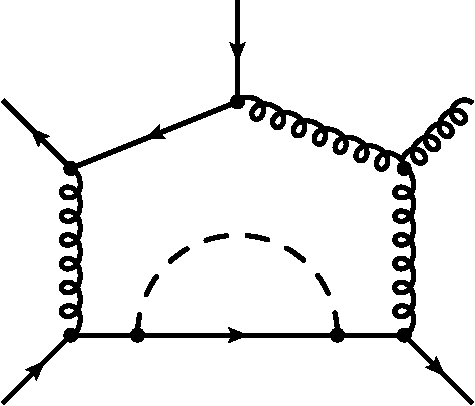
\includegraphics[width=\diagramWidth]{figures/Ds-example-1-2.pdf}}}
    ~\Big) ~\cdot~ (D_s-6) \quad +\\
    &
    \vcenter{\hbox{\includegraphics[width=\diagramWidth]{figures/Ds-example-2.pdf}}}
    ~\cdot~ (D_s-6)^2,
  \end{align*}
  \caption{Example of diagrams with scalar particles,
    representing the contributions to the coefficients of $\tilde{\mathcal{K}}_i$ in eq.~\eqref{eq:ds-poly-alt}.
    The thick lines in the diagram on the left-hand side represent particles in arbitrary $D_s$ dimensions.
    The (red) dashed lines connecting external-quark lines represent the traces required to obtain the coefficient of the tensor structure of eq.~\eqref{eq:defAmpsTensb}.
    All particles on the right-hand side are in six dimensions.}
  \label{fig:ds-example-diagram}
\end{figure}


We would like to conclude this section with some remarks.
First, the remaining non-trivial traces of eq.~\eqref{eq:ds-split-traces},
i.e.\ those of $\prod_k\gamma^{\mu_k}_{[6]}$, cannot be simplified generically
as the indices appear contracted with the loop momenta at the integrand level.
We evaluate them by the direct summation over a specially constructed set of external states
(in an analogous way to the sums performed in~\cite{Abreu:2018jgq} 
for dimensional reconstruction).
Secondly, in the absence of fermions in the loops, this method coincides with the so called
six-dimensional formalism employed in refs.~\cite{Badger:2013gxa,Badger:2017jhb}, and can 
thus be viewed as an extension thereof to amplitudes with fermions.
Finally, we note that the method presented in this section can be straightforwardly
generalized to higher number of loops by adjusting the base dimension $D_0$,
as well as to the extraction of coefficients of different tensor structures in 
eq.~\eqref{eq:tensorDecomposition}.



\subsection{Unitarity-Compatible Implementation}
decomposition of trees through simplified off-shell recursion.
    Collecting $(D_s-6)$ powers and factors. Implementation in process libraries.

    \todo{Use tree example here}




%%-------------------------------------------------


%\chapter{Renormalization}
%\label{chap:renorm}
%In order to arrive at physical predictions, we need to
\textit{renormalize} QCD \ola s. Renormalization refers to the process of
connecting the initial Lagrangian parameters, so called bare
parameters, to physical quantities that can be measured in experiment. In a renormalizable theory, UV divergencies stemming from
virtual corrections drop out once the bare parameters are connected to
physical ones. The SM, and thus QCD, is a renormalizable theory \cite{tHooft:1971qjg,tHooft:1972tcz}.


We renormalize \ola s for processes involving massive quarks in a
mixed scheme. The strong coupling is renormalized in the
$\MSb$ scheme
and we apply a shift to decouple massive quark loops from the running of
$\alpha_s$. The wave-function and mass renormalization is done in the
on-shell scheme. The mass renormalization is performed at the
level of each color-ordered amplitude. Previously, we explicitly broke gauge invariance of the amplitudes by
removing external leg self-energy Feynman diagrams from tree
amplitudes that appeared in double cuts on \olb~topologies
(cf.~Sec.~\ref{sec:massivebubble}). After recombination with the corresponding mass counterterms, gauge
invariance of the \ola s is restored. The coupling renormalization and massive quark
decoupling as well as wave-function renormalization lead to a shift proportional to the tree amplitude. We provide all renormalization constants in FDH to
be consistent with the computation of the \ola s. 

Furthermore, in Sec.~\ref{sec:scaledep} we work out the correct \root~\cite{ROOT} \ntuple{} weights \cite{BH:Ntuples} for massive
one-loop amplitudes. Using \ntuple{} files allows for an efficient a-posteriori reevaluation of
matrix elements with different renormalization and factorization
scales as well as couplings and parton distribution functions.

\section{Multiplicative Renormalization}
\label{sec:stdrenorm}
We will briefly review the standard multiplicative renormalization
procedure (more details can be found in many textbooks \cite{PeskinS,Schwartz:2013pla,Bohm:2001yx}). In particular, we will see that mass counterterms have to
be computed at the level of each color-ordered amplitude whereas the
other renormalizations result in a shift proportional to the tree amplitude. We
reparameterize the bare parameters in the Lagrangian by 
\begin{align}
  \psi_0 & = \sqrt{Z_2}\psi_R, & A_0^\mu & =  \sqrt{Z_3} A_R^\mu, \\
m_0 & = Z_m m_R, & g_0 & = Z_g g_R, \notag
\end{align}
where $\psi_0$ is the bare fermion field, $A^\mu_0$ the bare QCD gauge field, $m_0$
the bare mass and $g_0$ the bare strong coupling. In perturbation
theory, we expand the renormalization constants $Z_i$ and get to first order
\begin{align}\label{eq:renconst}
  Z_2 & \equiv 1 + \delta_2, &  Z_3 &\equiv 1 + \delta_3,  \\
  Z_m & \equiv 1 + \delta_m, &  Z_g &\equiv 1 + \delta_g, \notag 
\end{align}
which leads to a split up of the Lagrangian. We get the
original Lagrangian in which bare parameters are replaced by
renormalized ones, and in addition, the so called \textit{counterterm}
Lagrangian that collects all terms in the renormalization constants $\delta_i$
and generates counterterm Feynman rules. The renormalization constants
multiplying the counterterm Feynman rules for QCD vertices are given by
\begin{align}\label{eq:vertqcdct}
\begin{split}
  Z_{3g}-1 = Z_3^{3/2}Z_g-1 &\equiv \frac{3}{2} \delta_3 +
  \delta_g, \\
  Z_{4g}-1 = Z_3^{4/2}Z_g^2 -1&\equiv  2\delta_3 + 2 \delta_g, \\
Z_{2q1g} -1= Z_2 Z_3^{1/2}Z_g -1 &\equiv  \delta_2 +
  \frac{1}{2}\delta_3 + \delta_g,
\end{split}
\end{align}
for the three- and four-valent gluon interaction $Z_{3g}$ and $Z_{4g}$
as well as the quark-gluon interaction $Z_{2q1g}$. The Feynman
rules for two-particle counterterms in Feynman gauge are given in Fig.~\ref{fig:qcdct}.
\begin{eqnarray*}
\begin{tikzpicture}[baseline=(m)]
  \begin{feynman}[inline=(m)]
    \vertex (m) at (0,0);
    \vertex (v1) at (1,0);
    \vertex (v2) at (2,0);
    \diagram* {
      (m)  -- [fermion,insertion={[size=8pt]0.99}] (v1) -- [fermion] (v2), 
    };
  \end{feynman}
\end{tikzpicture}
 & \qquad i\left((\slashed{p}-m_R)\delta_2 -
\delta_mm_R\right) &=P^q_{\text{ct}}(p)_{|\delta_2} +P^q_{\text{ct}}(p)_{|\delta_m}\\
\vspace{1cm}
\begin{tikzpicture}[baseline=(m)]
  \begin{feynman}[inline=(m)]
    \vertex (m) at (0,0);
    \vertex (v2) at (2,0);
    \diagram* {
      (m)  -- [gluon,insertion={[size=8pt]0.5}] (v2), 
    };
  \end{feynman}
\end{tikzpicture}& \qquad -ip^2\delta_3 g^{\mu\nu}&=P^{g,\mu\nu}_{\text{ct}}(p)\\
\end{eqnarray*}
\vspace{-1.5cm}
\captionedequationset{Feynman rules for QCD two-particle counterterms in Feynman gauge. The renormalization constants
  $\delta_i$ are defined in Eq.~\eqref{eq:renconst}.\label{fig:qcdct}} 
In principle, one has to compute all possible
counterterms as specified by the counterterm Feynman rules. However,
the simple counting exercise of Sec.~\ref{sec:renorm-shifts-prop} reveals that wave-function and coupling renormalization of QCD one-loop amplitudes lead to a
renormalization shift proportional to the tree. The remaining mass
renormalization counterterms have to be computed explicitly, as
spelled out in Sec.~\ref{sec:mrenorm}.

\section{Coupling and Wave-Function Renormalization}
\label{sec:renorm-prop-tree}

\subsection{Renormalization Shifts Proportional to Tree Amplitudes}
\label{sec:renorm-shifts-prop}

We first observe that the combination of two propagators of the QCD spectrum with a counterterm
insertion leads, for the parts independent of $\delta_m$, to the original propagator
multiplied by a renormalization constant. In particular, the counterterm
insertion on fermion propagators is given by
\begin{align}\label{eq:repropq}
\begin{split}
  P^q(p)P_{\text{ct}}^q(p)_{|\delta_2} P^q(p)& =  \frac{i(\slashed{p}+m_R)}{p^2-m_R^2}\left(i(\slashed{p}-m_R)\delta_2\right) \frac{i(\slashed{p}+m_R)}{p^2-m_R^2}\\
  &=-\delta_2\frac{i(\slashed{p}+m_R)}{p^2-m_R^2} = -\delta_2 P^q(p),
\end{split}
\end{align}
and that on gluon propagators by
\begin{align}\label{eq:repropg}
\begin{split}
  P^g_{\mu\nu}(p) P^{g,\nu\rho}_{\text{ct}} P^g_{\rho\sigma}(p)& =  \frac{-ig_{\mu\nu}}{p^2} \left(-ip^2\delta_3 g^{\nu\rho}\right)  \frac{-ig_{\rho\sigma}}{p^2}\\
  &=-\delta_3\frac{-ig_{\mu\sigma}}{p^2} = -\delta_3P^g_{\mu\sigma}(p).
\end{split}
\end{align}
It remains to show that the multiplicative renormalization factor of each Feynman diagram is
purely determined by the number and species of external particles. In
order to do so, we count vertices and
propagators of QCD tree amplitudes and multiply them with the corresponding
renormalization factors,
cf.~Eqs.~\eqref{eq:vertqcdct}-\eqref{eq:repropg}. We start with pure gluon amplitudes with $n$
external particles. For each Feynman diagram contributing to the
amplitude, we have
\begin{align}\label{eq:gvert}
  n = n_3 + 2 n_4 + 2,
\end{align}
where $n_3$ and $n_4$ are the number of three- and four-valent gluon
interactions. The number of gluon propagators $n_{\text{p,g}}$ is
related to the number of vertices by
\begin{align}\label{eq:gprop}
  n_{\text{p,g}} = n_3+ n_4 -1.
\end{align}
Therefore, the renormalization constants multiplying each Feynman
diagram are given by
\begin{align}
\begin{split}
  \text{R}(n,n_3,n_4,n_{\text{p,g}}) &= n_4 \left( 2\delta_3 + 2\delta_g \right) +n_3 \left(
    \frac{3}{2} \delta_3 + \delta_g \right)-n_{\text{p,g}} \delta_3\\
%&= n_4 \left( 2\delta_3 + 2\delta_g \right) +( n - 2 n_4 - 2) \left(
%    \frac{3}{2} \delta_3 + \delta_g \right)-(n - n_4 -3)\delta_3 \\
&= \frac{n}{2}\delta_3 +(n-2)\delta_g \equiv \text{R}(n),
\end{split}
\end{align}
where we used Eqs.~\eqref{eq:gvert} and \eqref{eq:gprop} as well as
the counterterm Feynman rules. Thus the renormalization constants
multiplying each Feynman diagram are only dependent on the number of
external legs. Wave-function
and coupling renormalization of pure gluon amplitudes are therefore
proportional to the corresponding tree
amplitude. 

We perform a similar counting exercise for processes involving both quarks and gluons. For a Feynman diagram of $n$ particles, with $N_g$ gluons, $N_q$ quarks, $n_3$ and $n_4$ gluon vertices and
$n_{\text{qg}}$ quark-gluon vertices, we get the relation
\begin{align}\label{eq:rqgen}
  n=N_g+N_q = n_3 + 2n_4 + n_{\text{qg}} +2.
\end{align}
The number of both gluon ($n_{\text{p,g}}$) and quark ($n_{\text{p,q}}$) propagators is given by
\begin{align}\label{eq:propqre}
  n_{\text{p,g}} &= n_3+n_4 + \left(\frac{N_q}{2} - 1\right), &   n_{\text{p,q}} &=
  n_{\text{qg}}-1- \left( \frac{N_q}{2} - 1\right).
\end{align}
The multiplicative renormalization factor $\text{R}(N_g,N_q,n_3,n_4,n_{\text{qg}},n_{\text{p,g}},n_{\text{p,q}})$ of each Feynman diagram with $N_g$ gluons and
$N_q$ quarks therefore reads
\begin{align}\label{eq:shiftfd}
\begin{split}
 \text{R}(\cdots) &= n_4 \left( 2\delta_3 + 2\delta_g \right) +n_3 \left(
    \frac{3}{2} \delta_3 + \delta_g \right)+n_{\text{qg}}\left(\delta_2+\frac{1}{2}\delta_3+\delta_g\right)-n_{\text{p,g}} \delta_3-n_{\text{p,q}} \delta_2\\
%&= n_4 \left( 2\delta_3 + 2\delta_g \right) +( n - 2 n_4 -n_{\text{qg}}+ (N_q-2)) \left(\frac{3}{2} \delta_3 +\delta_g \right)+n_{\text{qg}}(\delta_2+\frac{1}{2}\delta_3+\delta_g)\\
%&\phantom{m}-\left(n -n_4-n_{\text{qg}} + \frac{1}{2}(m - 2)\right) \delta_3-\left(n_{\text{qg}}-\frac{m}{2} \right) \delta_2\\
&=\frac{N_g}{2}\delta_3
+\frac{N_q}{2}\delta_2+\left(n-2\right)\delta_g \\
&\equiv \text{R}(N_g,N_q),
\end{split}
\end{align}
where we have used Eqs.~\eqref{eq:rqgen} and \eqref{eq:propqre} and
the counterterm Feynman rules. As above, the wave-function and coupling renormalization shift for
amplitudes containing quarks and gluons is proportional to a
tree amplitude.

\subsection{Renormalization Constants}
\subsubsection{Gluon Wave-Function Renormalization}
We renormalize the gluon wave function in the on-shell scheme. The
renormalization constant is fixed by the requirement that the residue
of the gluon propagator is one. As a side effect, we do not have
to calculate self-energy corrections on external gluon legs. The
renormalization constant in the on-shell scheme calculated in FDH is
given by
\begin{align}
Z_3^{\text{os}}=1+\delta_{3}=1-g_s^2c_\Gamma\frac{2}{3}\left(\frac{1}{\epsilon} +
  \log\left(\frac{\mu^2}{ m_{\text{os}}^2}\right)\right)+\mathcal{O}(g_s^4,\epsilon),
\end{align}
with a heavy quark with on-shell mass $m_{\text{os}}$ running in the
closed loop and the prefactor $\displaystyle
c_\Gamma=(4\pi)^{-(2-\epsilon)}\Gamma(1+\epsilon)\Gamma^2(1-\epsilon)/\Gamma(1-2\epsilon)$
appearing in all integrals and renormalization constants. As we saw
in Eq.~\eqref{eq:shiftfd}, each of the $N_g$ external gluons contributes a
factor of $\frac{1}{2}\delta_3$ and we get contributions from each
flavor in closed massive quark loops. Therefore the
renormalization shift to a \ola~involving $n$ particles and $N_g$ gluons is given by
\begin{align}
\begin{split}
  \text{R}_{\text{wf, gluon}} &= -g_s^{2}c_\Gamma
N_g\sum_{i=1}^{N_{hf}}\left(\frac{1}{3\epsilon} + 
  \frac{1}{3}\log\left(\frac{\mu^2}{ m_{i,\text{os}}^2}\right)\right)
\Ampt(1,\dots,n)\\
&=-g_s^{2}c_\Gamma
N_g \Delta_3 \Ampt(1,\dots,n),
\end{split}
\end{align}
where $N_{hf}$ denotes the number of heavy-quark flavors with mass $m_{i,\text{os}}$.
%There is no contribution from massless quarks to the gluon
%self-energy, since the corresponding integrals vanish in dimensional regularization.
\subsubsection{Massive Quark Wave-Function Renormalization}
 We use the on-shell scheme to renormalize the massive quark wave
 function and the renormalization constant in FDH is given by
\begin{align}
 Z_2^{\text{os}}=1+\delta_2&=1-g_s^2c_\Gamma C_F\left(\frac{3}{\epsilon}+3\log{\left(\frac{\mu^2}{m_{\text{os}}^2}\right)}+5\right)+\mathcal{O}(g_s^4,\epsilon),
\end{align}
with $C_F=\frac{N_C^2-1}{2N_C}$. 
%The constant $Z_2^{\text{os}}$ is fixed from requirements on the fermion propagator Eq.~\eqref{eq:osfermprop}.
%\begin{align}
% \lim_{p^2\rightarrow m^2_{\text{os}}}\left[\frac{i(\slashed{p}+m_{\text{os}})}{p^2-m^2_{\text{os}}}\left(1-{\hat\Sigma}_0(\slashed{p})-\frac{m_{\text{os}}(\slashed{p}+m_{\text{os}})\tilde{\Sigma}_1(\slashed{p})}{p^2-m_{\text{os}}^2}\right)u(p)\overset{!}{=}\frac{i(\slashed{p}+m_{\text{os}})}{p^2-m^2_{\text{os}}}u(p)\right],
%\end{align}
%which can be rephrased as
%\begin{align}
%  \hat\Sigma_0(m_{\text{os}}^2)+2m^2_{\text{os}}\tilde{\Sigma}^\prime_1(m_{\text{os}}^2)=0,
%\end{align}
%with the self-energies $\Sigma_i$ defined as in Sec.~\ref{sec:mrenorm} and
%$\Sigma^\prime(\slashed{p})=\pdv{\Sigma(\slashed{p})}{\slashed{p}}$. 
Each massive external fermion
contributes a factor of $\frac{1}{2}\delta_2$, see Eq.~\eqref{eq:shiftfd}. Therefore, the
renormalization shift to a \ola~involving $n$ particles including external massive quarks is given by
\begin{align}
\begin{split}
  \text{R}_{\text{wf, quark}} &= -g_s^{2}c_\Gamma
\sum_{i=1}^{N_{hf}}N_{Q_i}\frac{1}{2}C_F\left(\frac{3}{\epsilon}+3\log{\left(\frac{\mu^2}{m_{i,\text{os}}^2}\right)}+5\right)\Ampt(1,\dots,n)\\
&= -g_s^{2}c_\Gamma
\sum_{i=1}^{N_{hf}}N_{Q_i}\frac{\Delta_{2,i}}{2}\Ampt(1,\dots,n),
\end{split}
\end{align}
where $N_{hf}$ denotes the number of heavy-quark flavors and $N_{Q_i}$ the number of external quarks of flavor $i$ with on-shell mass $m_{i,\text{os}}$.

%See for example:\\
%KST, \url{https://arxiv.org/pdf/hep-ph/9305239.pdf}\\
%\url{https://arxiv.org/pdf/0807.4424.pdf}\\
%\url{https://arxiv.org/pdf/hep-ph/9310301.pdf}\\
%Weinzierl, \url{https://arxiv.org/pdf/hep-ph/0207055.pdf}

\subsubsection{Coupling Renormalization}
The coupling renormalization constant is fixed by a
calculation of the
vacuum polarization. We use the $\MSb$ scheme, where the
renormalization constant for the coupling computed in FDH is given by
\begin{align}
 Z_g^{\MSb}=1+\delta_g=1-g_s^2c_\Gamma\frac{1}{2}\left(\frac{11\NC-2(\NF+N_{hf})}{3\epsilon}-\frac{\NC}{3}\right)
 + \mathcal{O}(\epsilon,g_s^4),
\end{align}
with $\NF$ denoting the number of light and $N_{hf}$ the
number of heavy-quark flavors. The finite shift $\frac{\NC}{3}$ stems
from the translation of the gauge coupling from standard $\MSb$ to the
FDH variant. As we saw in Eq.~\eqref{eq:shiftfd}, each power $N_{g_s}$ of the strong coupling $g_s$ contributes to the renormalization shift
\begin{align}
\begin{split}
 \text{R}_{\text{coupling}} &= -g_s^{2}c_\Gamma \frac{N_{g_s}}{2}
 \left(\frac{11\NC-2(\NF+N_{hf})}{3\epsilon}-\frac{\NC}{3}\right)\Ampt(1,\dots,n)\\
 &= -g_s^{2}c_\Gamma N_{\alps} \Delta_{\alps}\Ampt(1,\dots,n).
\end{split}
\end{align}
For pure QCD amplitudes, the power of $g_s$ is given by
$N_{g_s}=n-2$ and that of $\alps$ by $N_{\alps}=N_{g_s}/2$. For amplitudes
involving \ew~gauge bosons, the counting is reduced accordingly.
\subsubsection{Heavy-Quark Decoupling}
We work in the decoupling scheme \cite{Collins1978a}. That is, we require
that heavy quarks decouple from the running of
$\alpha_s$ at energies $E\ll m_{hf}$. Consequently, the appropriate $\MSb$ coefficients for the
running of $\alpha_s$ should be the same as in absence of the heavy
quarks. Therefore, diagrams with a heavy quark loop
are subtracted at zero momentum transfer and the decoupling shift for an
$n$-particle amplitude with $\frac{n-2}{2}$ powers of the strong
coupling $\alps$ and $N_{hf}$ decoupled heavy-quark flavors is
given by
\begin{align}
\begin{split}
\text{R}_{\text{decoupling}}&= g_s^{2}c_\Gamma
N_{\alps}\sum_{i=1}^{N_{hf}}
\frac{2}{3}\log(\frac{\mu^2}{m_{i,\text{os}}}) \Ampt(1,\dots,n)\\
&= -g_s^{2}c_\Gamma N_{\alps}\sum_{i=1}^{N_{hf}}
\Delta_i\Ampt(1,\dots,n),
\end{split}
\end{align}
where the sum runs over heavy quark flavors $N_{hf}$ and $N_{\alps}$ denotes the power of the coupling $\alps$. For processes involving \ew~gauge bosons, the counting is
reduced accordingly.
%\url{http://lanl.arxiv.org/pdf/hep-ph/0508242}
%\url{https://ac.els-cdn.com/0550321382900384/1-s2.0-0550321382900384-main.pdf?_tid=3fc95d9e-a468-11e7-b8d4-00000aacb362&acdnat=1506615511_0873854316f0722bef4a45c5ee57e85d}

\section{Mass Renormalization}
\label{sec:mrenorm}
For processes involving massive quarks, we need to renormalize the
bare mass parameter. Its renormalization cannot be represented
as a contribution proportional to the tree amplitude. For convenience we combine the computation of these
contributions with the bubble diagrams. We explicitly
compute mass-counterterm contributions using a dedicated recursive
tree-like computation at the level of primitive loop amplitudes. The only source to the $\delta_m$ counterterm is the two-particle QCD counterterm interaction, cf.~Fig.~\ref{fig:qcdct} and Eq.~\eqref{eq:vertqcdct} 
\begin{align}\label{eq:fermionpropins}
  P^q_{\text{ct}}(p)_{|\delta_m} = -im_R \delta_m.
\end{align}
For double cut topologies with a gluon and a massive quark
cut line, the mass counterterm is computed by replacing the two cut lines of the bubble with fermion propagators and the above insertion of
Eq.~\eqref{eq:fermionpropins} as shown in Fig.~\ref{fig:massct}. The counterterm for a double cut topology
with legs $1_g,\dots,j_{\bar{q}}$ joining in vertex one and
$(j+1)_g,\dots,n_q$ in vertex two is thus computed by
\begin{align}
  \text{CT}_{1_g,\dots,j_{\bar{q}};(j+1)_g,\dots,n_q} =
  Q(1_g,\dots,j_{\bar{q}}) P^q_{\text{ct}}(P_{1j})_{|\delta_m} \bar{Q}((j+1)_g,\dots,n_q),
\end{align}
where we denoted the momentum sum $P_{ij}=\sum_{k=i}^jp_k$ and $Q$ and
$\bar{Q}$ denote quark and anti-quark Berends-Giele currents respectively. By adding these
counterterms to each color-ordered \ola, gauge invariance is
restored at the level of primitive amplitudes, after initially being broken by the removal of external leg self-energy insertions in \olb~cuts, cf.~Sec.~\ref{sec:massivebubble}.
\begin{equation*}
\begin{tikzpicture}[baseline=(m1)]
  \def\leglength{1}
  \def\blobpos{2.5}
  \def\cutshift{0.3}
  \def\cutlength{1.0}

  %The double cut lines
  \pgfmathsetmacro\vertcut{(\blobpos-1)/2+1}
  \draw[very thick] (\vertcut,\cutshift) -- (\vertcut,\cutshift+\cutlength);
  \draw[very thick] (\vertcut,-\cutshift) -- (\vertcut,-\cutshift-\cutlength);

  %\node at (-0.3,0) {\(1_{\bar{q}}\)};
  \begin{feynman}[inline=(m1)]
    \vertex[blob] (m) at (\blobpos, 0) {};
    \vertex[blob] (m1) at (1, 0){};
    \vertex (i) at (0, 0){\(\vdots\)};
    \vertex (i1) at (0, \leglength){\(j_{\bar{q}}\)};
    \vertex (i2) at (0, -\leglength){\(1_g\)};
    \vertex (a) at (\blobpos+\leglength,0){\(\vdots\)};
    \vertex (b) at (\blobpos+ \leglength,\leglength){\( (j+1)_{g} \)};
    \vertex (c) at (\blobpos+ \leglength,- \leglength){\(n_{q}\)};
    \diagram* {
     (m1) -- [gluon, half left,out=90,in=90] (m)
       -- [half left, thick,out=85,in=95] (m1),
       (m) -- [gluon] (b),
       (m1) -- [anti fermion] (i1),
       (m1) -- [gluon] (i2),
      (m) -- [fermion,  thick] (c),
    };
  \end{feynman}
\end{tikzpicture}
\hspace{0.5cm}\longrightarrow\hspace{0.5cm}
\begin{tikzpicture}[baseline=(m1)]
  \def\leglength{1}
  \def\blobpos{3.5}
  \def\cutshift{0.3}
  \def\cutlength{1.0}

  %\node at (-0.3,0) {\(1_{\bar{q}}\)};
  \begin{feynman}[inline=(m1)]
    \vertex[blob] (m) at (\blobpos, 0) {};
    \vertex[blob] (m1) at (1, 0){};
    \vertex (mi) at (2.25, 0);
    \vertex (i) at (0, 0){\(\vdots\)};
    \vertex (i1) at (0, \leglength){\(j_{\bar{q}}\)};
    \vertex (i2) at (0, -\leglength){\(1_g\)};
    \vertex (a) at (\blobpos+\leglength,0){\(\vdots\)};
    \vertex (b) at (\blobpos+ \leglength,\leglength){\( (j+1)_{g} \)};
    \vertex (c) at (\blobpos+ \leglength,- \leglength){\(n_{q}\)};
    \diagram* {
      (m1) -- [fermion,insertion={[size=8pt]0.99}] (mi)   -- [fermion] (m),
       (m) -- [gluon] (b),
       (m1) -- [anti fermion] (i1),
       (m1) -- [gluon] (i2),
      (m) -- [fermion,  thick] (c),
    };
  \end{feynman}
\end{tikzpicture}
\end{equation*}
\vspace{-1.2cm}
\captionedequationset{Generation of mass counterterms. For double cut
  topologies with a gluon and fermion cut line, we compute the
  corresponding counterterm by joining the two currents
  $Q(1_g,\dots,j_{\bar{q}})$ and $\bar{Q}((j+1)_g,\dots,n_q)$ with the
  fermion two-particle counterterm interaction.\label{fig:massct}} 


We renormalize the mass in the \textit{on-shell scheme}. The renormalization
constant $Z_m$, computed in Feynman gauge and expressed in FDH is given by
\begin{align}\label{eq:rcm}
\begin{split}
  Z_m^{\text{os}}=1+\delta_m&=1-C_Fg_s^2c_\Gamma
  \left(\frac{\mu^2}{m_{\text{os}}^2}\right)^\epsilon
  \left(\frac{3}{\epsilon}+5\right)+\mathcal{O}(g_s^4)\\
&=1-C_Fg_s^2c_\Gamma \left(\frac{3}{\epsilon}+3\log{\left(\frac{\mu^2}{m_{\text{os}}^2}\right)}+5\right)+\mathcal{O}(g_s^4,\epsilon).
\end{split}
\end{align}
The color factor $C_F$ evaluates to $C_F=1$ if we compute the counter
terms for color-ordered particles. In the
on-shell scheme, the renormalization constant
$Z_m^{\text{os}}$ is fixed such that the pole of the
propagator is described by the renormalized mass
$m_{\text{os}}$, thereby fixing the finite terms. 

%Summing up the one-particle irreducible contributions
%to the fermion propagator up to first order, we get
%\begin{align}\label{eq:osfermprop}
%\begin{split}
%  \hat{P}^q(p)&=\frac{i(\slashed{p}+m_R)}{p^2-m^2_R}\left(1-\frac{(\slashed{p}+m_R)\hat\Sigma(\slashed{p})}{p^2-m_R^2}\right)\\
%&=\frac{i(\slashed{p}+m_R)}{p^2-m^2_R}\left(1-{\hat\Sigma}_0(\slashed{p})-\frac{m_R(\slashed{p}+m_R)\tilde{\Sigma}_1(\slashed{p})}{p^2-m_R^2}\right),
%\end{split}
%\end{align}
%where we denote renormalized quantities with a hat. The renormalized
%self-energy $\hat\Sigma(\slashed{p})$ can be split into vectorial and scalar part
%according to $\hat\Sigma(\slashed{p})=\slashed{p}{\hat\Sigma}_0(\slashed{p})+m{\hat\Sigma}_1(\slashed{p})$ and the sum of the
%parts is denoted by
%$\tilde{\Sigma}_1(\slashed{p})={\hat\Sigma}_0(\slashed{p})+{\hat\Sigma}_1(\slashed{p})$. If we then require
%to have a simple pole in Eq.~\eqref{eq:osfermprop} for $p^2\rightarrow m_R\equiv m_{\text{os}}$, we obtain the renormalization condition
%\begin{align}\label{eq:rnc1}
%  \lim_{p^2\rightarrow m^2_{\text{os}}}\tilde{\Sigma}_1(p^2) = \tilde{\Sigma}_1(m_{\text{os}}^2)  = 0.
%\end{align}
%The sum of renormalized self-energies
%${\tilde\Sigma}_1(m_{\text{os}}^2)$ written in terms of unrenormalized
%self-energies is given by
%\begin{align}
%\begin{split}
%  \tilde{\Sigma}_1(m_{\text{os}}^2) &=
%  {\hat{\Sigma}}_0(m_{\text{os}}^2)+{\hat \Sigma}_1(m_{\text{os}}^2) \\
%&=  {\Sigma}_0(m_{\text{os}}^2)+{\Sigma}_1(m_{\text{os}}^2)-\delta_{m}^{\text{os}}=0,
%\end{split}
%\end{align}
%which fixes the finite part of $Z_m^{os}\equiv
%1+\delta_{m}^{\text{os}}$. It evaluates in FDH to Eq.~\eqref{eq:rcm}, given the expressions for the unrenormalized quark
%self-energies in QCD.



%\subsection{$\gamma_5$ renormalization}
%In the HV scheme we do have a finite shift for $gamma_5$.
%\begin{align}
%  \gamma^\mu\gamma_5 \rightarrow   \frac{1}{2} Z_{axial}(\gamma^\mu\gamma_5 -  \gamma_5\gamma^\mu)\notag
%\end{align}
%with $Z_{axial}=1-2C_F 1_{HV}$\\
%\url{https://arxiv.org/pdf/hep-ph/9903380.pdf}

\section{Summary of Renormalization}
\label{sec:summary}
In summary, we renormalize \ola s in a mixed scheme. For external states we use the on-shell
scheme and the gluon wave-function renormalization receives contributions from all
active heavy quark flavors. We renormalize the mass in the on-shell scheme
and compute mass renormalization counterterms
explicitly at the level of each color-ordered amplitude. The QCD coupling is renormalized in $\MSb$, where we decouple massive quarks from the
running of $\alpha_s$. The renormalized \ola~is obtained by combining all tree-like renormalization shifts with the mass renormalized \ola
\begin{align}
\begin{split}
  \Amp_{(ren)}&=
  \Amp_{(mass\
    ren)}+\text{R}_{\text{wf,quark}}+\text{R}_{\text{wf,gluon}}+\text{R}_{\text{coupling}}+\text{R}_{\text{decoupling}}\\
&= \Amp_{(mass\
    ren)}-g_s^2 c_\Gamma \left( \sum_{i=1}^{N_{hf}} N_{Q_i} \frac{\Delta_{2,i}}{2} + N_{g}\Delta_3 +
    N_{\alps}\left(\Delta_{\alps} + \sum_{i=1}^{N_{hf}}\Delta_i\right) \right)  \mathcal{A}^{\text{tree}},
\end{split}
\end{align}
where $N_{hf}$ denotes the number of heavy flavors, $N_{Q_i}$ the number of external heavy quarks of flavor $i$, $N_g$ the number of external
gluons and $N_{\alps}$ the power of $\alps$ (at Born level) . The
renormalization constants in the FDH scheme are summarized in Table \ref{tab:renorm}.
\begin{table}[h]
  \caption{Renormalization constants used in this thesis. Here $\mu$ is the renormalization
  scale, $m_{i}$ are the masses for heavy quarks, $\NF$ is the number of light flavors,
  $N_{hf}$ the number of heavy flavors, and $\NC$ the number of colors.
  A common factor of $-g_s^2 c_\Gamma$ has been factored out.}
      \vskip 4mm
  \centering
    \begin{tabularx}{\textwidth}{lcll}
      \hline\hline
      \noalign{\vskip 4mm}
      \textbf{Renormalization} & \textbf{Scheme} & \textbf{Constant}\\
      \noalign{\vskip 3mm}
      \hline
      \noalign{\vskip 2mm}
      %\rule{0pt}{1ex}\\
    %\small
      %\toprule
      Heavy-quark wave function   & on-shell & $\displaystyle
      \Delta_{2,i} ~=~ \frac{\NC^2-1}{2\NC} \left( \frac{3}{\epsilon}
        + 3 \log{\frac{\mu^2}{m_i^2} + 5} \right)$\\
      \noalign{\vskip 1mm}
      Light-quark wave function   & on-shell & 0\qquad(UV+IR
      cancellation) \\
      \noalign{\vskip 3mm}
      Quark mass            & on-shell & $\displaystyle \Delta_{m_i}
      ~=~ \Delta_{2,i}\quad\text{}$\\
      \noalign{\vskip 1mm}
      Gluon wave function   & on-shell & $\displaystyle \Delta_3 ~=~ \sum_{i=1}^{N_{hf}}\left(\frac{1}{3 \epsilon} +
      \frac{1}{3}\log{\frac{\mu^2}{m_i^2}}\right)$\\
      \noalign{\vskip 1mm}
      QCD coupling & $\MSb$ & $\displaystyle \Delta_{\alps} ~=~  \frac{1}{\epsilon} \left( \frac{11}{3}\NC - \frac{2}{3}(\NF+N_{hf}) \right) - \frac{\NC}{3}$\\
      \noalign{\vskip 2mm}
      \hline
      \noalign{\vskip 2mm}
      Decoupling shift & --- & $\displaystyle     \Delta_i ~=~-
      \frac{2}{3}\log{\frac{\mu^2}{m_i^2}} $\\
      \noalign{\vskip 1mm}
      \hline\hline
    \end{tabularx}
  \label{tab:renorm}
\end{table}

\section{Scheme Shift From FDH to 't Hooft-Veltman}
\label{sec:schemeshift}
We use the FDH variant of dimensional regularization in intermediate steps to
regularize UV and IR divergences. At the end we convert the renormalized
amplitude to the HV scheme~\cite{tHooft:1972tcz} which is often more convenient for comparisons and interfacing with Monte-Carlo generators. The conversion of a renormalized \ola~$\Amp_{(ren)}$ is performed by a finite shift, see
e.g.\ \cite{Signer:2008va}
\begin{align}
  \mathcal{A}_{(ren)}^{\text{1-loop,HV}} =
  \mathcal{A}_{(ren)}^{\text{1-loop,FDH}} - g_s^{2}c_\Gamma\left(N_g\frac{\NC}{6}+N_q\frac{\NC^2-1}{4\NC}\right)\Ampt,
\end{align}
where $N_g$ denotes the number of gluons and $N_q$ the number of light
quarks in the respective amplitude.



\section{Scale Variation Using \Ntuple{} Data}
\label{sec:scaledep}

We provide NLO results in the form of \root~\cite{ROOT} \ntuple{} files \cite{BH:Ntuples}. The \ntuple{} files allow to reevaluate
generic IR-safe observables with different renormalization and
factorization scales as well as different PDFs. They store the relevant information to
reevaluate observables without recomputing the short-distance matrix
elements, which is possible due to the particular simple form of the parts of the virtual matrix element that depend on $\mu_R$. This possibility for a-posteriori variations of scales and PDFs
make the efficient estimation of uncertainties associated to NLO
predictions possible. 

In this section, we analyze the dependence of virtual cross sections on the unphysical renormalization scale. We neglect the implicit dependence
via the strong coupling for this discussion, since it amounts to a global prefactor and can be
treated as described in \cite{BH:Ntuples}. In particular, we identfiy additional
renormalization terms with $\mu_R$ dependence which are present in calculations with massive external particles and have to be considered in order to supply the correct data for \ntuple{} files.

The dependence of the virtual cross section on the unphysical scale
$\mu_R$ is introduced in
dimensional regularization to enforce a mass dimension of one for the
gauge 
couplings $g\rightarrow \mu_R^{\epsilon}g$. As a consequence, there is
an explicit dependence on $\mu_R$ in virtual NLO matrix elements. We can write an unrenormalized, one-loop
amplitude, with couplings stripped off, as
\begin{align}\label{eq:mudep}
  \Amp(\mu_R) =  \tilde{\mu}_R^{2\epsilon}\left[\frac{a_{2}}{\epsilon^2}+\frac{a_{1}}{\epsilon}
  + a_0\right],
\end{align}
where we use the dimensionless scale $\tilde{\mu}_R =
\frac{\mu_R}{\text{GeV}}$ to simplify the argument in the following. We generically have ratios of
renormalization scale $\mu_R$ and involved physical scales, from which
we build dimensionless quantities by
\begin{align}
 \left(\frac{\mu_R}{s}\right)^{2\epsilon} =\tilde{\mu}_R^{2\epsilon}\left(\frac{\text{GeV}}{s}\right)^{2\epsilon}.
\end{align}
Note, that Eq.~\eqref{eq:mudep} is valid for
any number of involved physical scales.
%\footnote{Assume we had two scales, the initial expression expression
%would be $ \sigma_V =
%(\frac{\mu_R}{sc_1})^{2\epsilon}\left[\frac{b_{2}}{\epsilon^2}+\frac{b_{1}}{\epsilon}
%+ b_0\right]+
%(\frac{\mu_R}{sc_2})^{2\epsilon}\left[\frac{c_{2}}{\epsilon^2}+\frac{c_{1}}{\epsilon}
%+ c_0\right]$. After identifying two identical dimensionless scales,
%we see that a redefinition of the parameters $b_i$ and $c_i$ leads to
%the form in Eq.~\eqref{eq:mudep}.}. 
We then expand $\left(\tilde{\mu}_R\right)^{2\epsilon}$ and obtain
\begin{align}
   \tilde{\mu}_R^{2\epsilon} = 1 +
   \log(\murt)\epsilon+\frac{1}{2}\log(\murt)^2\epsilon^2
   + \mathcal{O}(\epsilon^3),
\end{align}
such that the explicit $\tilde \mu_R$ dependence of
Eq.~\eqref{eq:mudep} becomes transparent
\begin{align}\label{eq:unrenam}
    \Amp(\mu_R)  = \left[\frac{a_{2}}{\epsilon^2}+\frac{a_{1}+a_{2}\log(\murt)}{\epsilon}
  + a_0+a_{1}\log(\murt)+\frac{1}{2}a_{2}\log(\murt)^2\right].
\end{align}
This formula contains double and single poles due to infrared
divergencies as well as single poles due to ultraviolet
divergencies. The difference of the finite part of the amplitude computed at two distinct scales $\mu_{R,1}$ and $\mu_{R,2}$ is then given by
\begin{align}\label{eq:extrapolscale}
\begin{split}
\Amp_{|\epsilon^{0}}({\mu}_{R,2}) -\Amp_{|\epsilon^{0}}({\mu}_{R,1})
  &=  a_1\log(\frac{\tilde{\mu}_{R,2}^2}{\tilde{\mu}_{R,1}^2})
+\frac{1}{2} a_2 \left[
    \log(\tilde{\mu}_{R,2}^2)^2-
    \log(\tilde{\mu}_{R,1}^2)^2\right]\\
&=  \left[a_1+a_2\log(\tilde{\mu}_{R,1}^2)\right]\log(\frac{\tilde{\mu}_{R,2}^2}{\tilde{\mu}_{R,1}^2})
+\frac{1}{2} a_2
\log(\frac{\tilde{\mu}_{R,2}^2}{\tilde{\mu}_{R,1}^2})^2,
\end{split}
\end{align}
which we can parameterize in terms of the weights $w_1$ and $w_2$
\begin{align}\label{eq:unrenweights}
  w_1 &\equiv a_{1}+a_2
  \log(\tilde{\mu}_{R,1}^2)=\Amp_{|\epsilon^{-1}},& w_2 &\equiv a_{2} = \Amp_{|\epsilon^{-2}}. 
\end{align}
The above parameterization has the advantage, that only ratios of
renormalization scales have to be considered and no explicit
dimensionless scales have to be constructed. The finite part of an unrenormalized \ola~at scale
$\tilde{\mu}_{R,2}$ can thus be extrapolated from that at scale
$\tilde{\mu}_{R,1}$ by adding the terms in Eq.~\eqref{eq:extrapolscale}
\begin{align}\label{eq:extrapolscale2}
\begin{split}
  \Amp_{|\epsilon^{0}}({\mu}_{R,2})   &= \Amp_{|\epsilon^{0}}({\mu}_{R,1}) +
  w_1\log(\frac{\tilde{\mu}_{R,2}^2}{\tilde{\mu}_{R,1}^2})+
\frac{1}{2} w_2
\log(\frac{\tilde{\mu}_{R,2}^2}{\tilde{\mu}_{R,1}^2})^2.
\end{split}
\end{align}
The above considerations are independent
of whether the involved particles are massive or not. In the
renormalization procedure, see the previous sections, additional
sources of $\mu_R$ dependence are introduced. Whereas mass and wave-function
renormalization lead to terms in which the logarithmic dependence in
the finite part has the same prefactor as the single pole, the shift
due to charge renormalization has no dependence on $\mu_R$ but
contributes to the single pole. Its
schematic contributions in an $\epsilon$ expansion
$(\epsilon^{-1},\epsilon^0)$ is given by
\begin{align}
   \text{R}_{\text{charge}} & = (a_{1,c},a_{0,c}),
\end{align} 
with coefficients $a_i$ that do not contain any logarithms. The decoupling
shift for massive quarks however has finite logarithms but no contribution
to the single pole
\begin{align}
   \text{R}_{\text{decoupling}} & = (0,a_{0,dec}\log(\murt)).
\end{align}
The weight $w_1$ should correctly parameterize simple logs of $\mu_R$ in
the finite part. To account for the absence of $\mu_R$ dependence in the charge renormalization and the fact that the decoupling shift
does not have a single-pole contribution, the weights for renormalized
amplitudes are defined as 
\begin{align}\label{eq:reweights}
 w_1 &=\Ampr_{|\epsilon^{-1}} -a_{1,c}+ a_{0,dec}, &  w_2 &= \Ampr_{|\epsilon^{-2}}.
\end{align}
With these weights, one can use Eq.~\eqref{eq:extrapolscale} to
extrapolate the virtual cross section to different values of $\mu_R$
for processes involving massive particles.

We provide the weights in Eq.~\eqref{eq:reweights} for each
phase space point together with the finite part of the matrix element squared. They
are stored in \ntuple{} files alongside information like the phase-space
point, the involved partons, the factorization and renormalization
scales, the Bjorken-x and the corresponding PDF
weights. We make extensive use of a-posteriori scale variations in the phenomenological
results presented in the following Chapters \ref{chap:wbb_intro}-\ref{chap:vjet_result}.


%%-------------------------------------------------

%\newpage
%\phantomsection
%\thispagestyle{empty}
%\vspace*{60 mm}
\begin{center}
{\Huge{\textbf{Part 2:}}}\\
\vspace*{5 mm}
{\Huge{\textbf{\texorpdfstring{$Wb\bar{b}+n$}{Wbb+n}~Jet Production
(\texorpdfstring{$n=0,1,2,3$}{n=0,1,2,3})}}}
\end{center}

%\addcontentsline{toc}{chapter}{{\large Part 2: \texorpdfstring{$Wb\bar{b}+n$}{Wbb+n}~Jet Production (\texorpdfstring{$n=0,1,2,3$}{n=0,1,2,3})}}

%%-------------------------------------------------

\chapter{NLO QCD Predictions for Production of \texorpdfstring{$Wb\bar b$}{Wbb} and Light Jets}
\label{chap:wbb_pheno}
In this chapter, we present one of the main results of this thesis:
the NLO QCD predictions for the production of \Wbb{} in association with up to three light jets.
We carry out the computation in the four-flavor-number scheme (4FNS), thus including effects due to the non-vanishing bottom-quark mass.
The motivation to undertake this challenging computation is two-fold.
Firstly, the class of processes we consider are important irreducible backgrounds to the recently discovered decay of the Higgs boson 
to a pair of bottom quarks, produced in association with heavy vector bosons \cite{Sirunyan:2018kst,Aaboud:2018zhk}.
By providing NLO QCD predictions in samples of light-jet multiplicity we hope to improve the theoretical 
understanding of the backgrounds, and, herewith, improve the measurements of the observables associated to 
the coupling of the Higgs boson to bottom quarks.
Secondly, understanding of one-loop numerical unitarity methods with massive particles
was an important stepping stone towards extending the computational techniques to a multi-loop setting,
and tackling much more complicated two-loop amplitudes in \cref{chap:5parton}.
In particular, the ideas of \cref{chap:dshel} have originally arisen from the necessity of the efficient
numerical evaluation of one-loop helicity amplitudes with external massive quarks.

This work is published in \cite{Anger:2017glm}, 
and the presentation in this chapter follows closely the one from the article.
In \cref{sec:wbb:relevance} we overview the status of theoretical and experimental studies of
the \Wbb{}+jets production, and its phenomenological relevance.
In \cref{sec:BHMassiveImpl} we briefly note on some of the
key developments we have implemented in a new version of the \BlackHat{} library,
which we employed to obtain the virtual matrix elements for this process.
In \cref{sec:wbb:setup} we discuss out computational setup for the Monte-Carlo integration
in \cref{sec:wbb:mc_integration}. Finally, in \cref{sec:wbb:pheno} we present our phenomenological studies.

\section{Introduction}
\label{sec:wbb:relevance}

The first NLO QCD theoretical studies of the \Wbb{} production were carried out in 
the context of the 4FNS in the approximation of massless bottom quarks about 20 years ago \cite{Bern:1997sc,Ellis:1998fv},
and were implemented in the first version of the MCFM program~\cite{mcfm7}.
The first results including the bottom-quark mass, but with on-shell $W$-boson 
appeared in \cite{FebresCordero:2006sj,Cordero:2009kv,Badger:2010mg,Oleari:2011ey}.
The phenomenological studies of NLO QCD \Wbbnj[1]{} production have be performed in \cite{Luisoni:2015mpa}.
Also, related studies of inclusive production of $W$-boson with a single $b$-tagged jet
can be found in \cite{Campbell:2006cu,Campbell:2008hh,Caola:2011pz}.
Finally, the signature of the process \Wbb{}+jets can be also produced from
the off-shell decays of the top quarks, which was studied in \cite{Denner:2017kzu}.
On the experimental side, several dedicated measurements
have been performed by the CDF \cite{Aaltonen:2009qi}, D0 \cite{D0:2012qt}, ATLAS \cite{Aad:2013vka}, and CMS \cite{Chatrchyan:2013uza,CMS:2016bb}
experiments.

In \cite{Anger:2017glm} we presented, for the first time, NLO QCD corrections to \Wbbnj[2]{} and
\Wbbnj[3]{} production. As illustrated in \cref{fig:wbb_channels} for an examples of $n=2$ light jets,
the final state signature we consider can be produced through different orders of the EW and strong couplings.
We study the QCD corrections of to the LO $\order{\alps^{2+n}\alpf^2}$ production,
which are the most important contribution outside of the single or double top-quark resonant regions.
Near the resonances the most important contributions are obtained from the QCD corrections to the LO $\order{\alps^{n}\alpf^4}$ production,
and EW corrections to the LO $\order{\alps^{1+n}\alpf^3}$. The latter were studied in \cite{Denner:2017kzu}.

\begin{figure}[t]
  \centering
  \includegraphics[width=0.8\textwidth]{wbb_channels}
  \caption{
    Different contributions to the $W(\to 2l)b\bar{b}jj$ final state.
    We consider the NLO QCD corrections to the channel with the least power of the EW coupling $\alpha$, which
    is dominant outside of the top-quark resonance region.
    The figure is based on \cite{Denner:2017kzu}.
  }
  \label{fig:wbb_channels}
\end{figure}


Already the firs studies of \Wbb{} production
recognized \cite{Ellis:1998fv,FebresCordero:2006sj,Cordero:2009kv} that the NLO QCD corrections are large. 
The main reasons are that the real radiation opens a new
gluon-induced production channel, and the that
the kinematical constraint on the transverse momentum of  $W$ is released.
These effects are collectively known as ``giant $K$-factors'' \cite{Rubin:2010xp}. 
Including an additional light jet in the final state improves the  behavior \cite{Luisoni:2015mpa}.
However only starting from \Wbbnj[2]{}, i.e.\ from two additional light jets, are all possible production
channels open at the LO.  We show that this in this case, as expected, the $K$-factors are moderate.


One of the first ideas to address the problem of large $K$-factors was exploiting the jet vetoes 
for more exclusive studies \cite{FebresCordero:2006sj}.
Unfortunately, the sensitivity to the $p_T^{\textrm veto}$ cut upsets
the precision  of the predictions in this case.
The latter can be mitigated by employing the so-called ``exclusive-sum'' techniques \cite{ESums},
which take advantage of the available multi-jet NLO samples.
In particular, we use them in \cref{sec:wbb:pheno} for our predictions of observables associated to the  $H(\rightarrow b{\bar b})W$ 
production: the $p_T^{b\bar b}$, $p_T^W$, and $M_{b\bar b}$ distributions.

%%%%%%%%%%%%%%%%%%%%%%%%%%%%%%%%%%%%%%%%%%%%

\section{Numerical Unitarity with Massive Particles in \BlackHat{}}
\label{sec:BHMassiveImpl}

The original version of the \texttt{C++} library \BlackHat{} \cite{Berger:2008sj,Berger:2008ag} has been
implemented having only massless QCD in mind. 
And the technical details went into that implementation are very different than
the multi-loop generalization we presented in \cref{chap:numunitarity}.
In this section we discuss the developments for the new version of \BlackHat{},
which has been required to be able to compute one-loop amplitudes with massive quarks.

A comprehensive review of the issues connected with the application of
one-loop numerical unitarity methods to massive particles can be found in \cite{Ellis:2011cr,Ellis:2008ir}.
Furthermore, some details of our implementation have been already discussed in \cite{FelixDiss},
so we limit ourselves to a very brief summary.

\paragraph{The strategy of handling the dimensional regularization}
was the most significant change.
The \BlackHat{} library was based on the numerical unitarity methods in four dimensions to extract the cut-constructable part
of the amplitude \cite{Ita:2011hi,Berger:2008sj,Berger:2008ag}. As for the rational part, either the special on-shell recursion, or the SUSY decomposition, have been employed.
Both approaches are not suitable for amplitudes with massive quarks.
To this end, we have reorganized the computation strategy to follow closer the $D$-dimensional unitarity method described in \cref{chap:numunitarity}\footnote{
  We did not, however, introduce the $D$-dependence into the coefficients as we did in the examples in \cref{sec:ms_examples}.
},
also taking advantage of our developments in \cref{chap:dshel} with some additional tricks explained in \cite{Anger:2018ove}.

Nevertheless, as an optimization opportunity,
we still extract the cut-constructable coefficients by sampling 
the cut equations \eqref{eq:cut_equations} 
with the four-dimensional loop momenta first.
We then transfer these coefficients to the left-hand side of \cref{eq:cut_equations} and use only a few additional
sample points with five-dimensional loop momenta to obtain the remaining coefficients.
This, in turn, implies that the general parametrization of on-shell loop-momenta, that we discussed in \cref{sec:evaluation_of_cuts},
is not suitable\footnote{
  it is also not suitable for the reason of numerical stability
}. For this reason we have constructed and implemented the on-shell loop-momenta parametrizations
for all topologies with massive particles in the loop, based on \cite{Kilgore:2007qr}.



\paragraph{The extraction of master coefficients} was previously organized according to a more analytics-oriented approach of \cite{Forde2007}.
With massive particles in the loop this approach becomes rather clunky.
Furthermore, we found that it does not offer any benefits over numerically-oriented OPP-like subtractions
in the cut equations \eqref{eq:cut_equations}. Therefore, we replaced the former by the latter.


\paragraph{Additional topologies.}
The tadpole and bubble topologies with the single on-shell particle in the corner (which we dub ``on-shell bubbles'')  no longer correspond to scaleless
integrals if massive particles are involved, hence they cannot be discarded.
We have implemented the construction of hierarchies for these topologies, as well the corresponding
on-shell loop-momentum parametrizations. 
In addition, there are some new features associated to these topologies:
\begin{enumerate}
  \item The cuts of all tadpoles and on-shell bubbles contain explicitly divergent contributions associated
    to the mass and wave-function renormalization (see \cref{fig:wbb:singdoublecut} for an example).
    We mentioned this towards the end of \cref{sec:cut_equations}.
    \begin{figure}[h]
      \[
        \vcenter{\hbox{\includegraphics[height=12ex]{./figures/dc_div_left.eps}}} =
        \vcenter{\hbox{\includegraphics[height=12ex]{./figures/dc_div_r.eps}}}~+~
        \vcenter{\hbox{\includegraphics[height=12ex]{./figures/dc_div2_cross.eps}}}
      \]
      \caption{
        A double cut with the single on-shell massive quark in the corner (on the left), containing
        a divergent contribution associated to the mass and wave-function renormalization (the second term on the right),
        which has to be manually removed.
      }
      \label{fig:wbb:singdoublecut}
    \end{figure}
    Following the approach of \cite{Ellis:2008ir} we have implemented the removal of this contributions in our off-shell recursion.

  \item The topology in \cref{fig:dc_div2}, in addition to containing a divergent contribution mentioned above,
    has another special feature: the transverse complement of its single light-like external momentum contains this momentum.
    We discussed this in \cref{sec:ms_examples}.
    \begin{figure}[h]
      \centering
      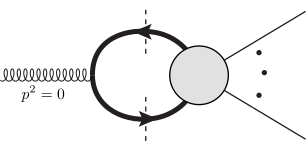
\includegraphics[width=0.3\textwidth]{dc_div2}
      \caption{A special one-loop topology with a massless on-shell leg in the corner and massive cut propagators.}
      \label{fig:dc_div2}
    \end{figure}
    This has two consequences. First, there are more coefficients with master integrals, and we evaluate the corresponding integrals explicitly.
    Second, as opposed to other one-loop topologies, the ansatz for the integrand of this topology is \emph{not} invariant under loop momentum shifts.
    This slightly complicates the construction of hierarchies, since it implies that the tadpoles below have to be carefully aligned.
    Interestingly, this is a generic feature beyond one loop, i.e.\ the ansätze for integrands of \emph{all} topologies are not invariant under loop momenta shifts.
\end{enumerate}


\paragraph{Integrals with internal masses.} Finally,
we have implemented all one-loop master integrals with real internal masses to $\order{\epsilon^0} $, based
on the results from \cite{Carrazza:2016gav,vanHameren:2010cp}. This allows us to incorporate
them in our automated numerical precision tracking and rescue system.

%%%%%%%%%%%%%%%%%%%%%%%%%%%%%%%%%%%%%%%%%%%%

\section{Setup}
\label{sec:wbb:setup}

\subsection{Channels}
\label{sec:calcsetup}

We compute NLO QCD corrections for the production of \Wbb~in association with $n$ light jets ($n =
0,1,2,3$) at the LHC $\sqrt{s} = 13$ TeV. 
We include the leptonic decays of the off-shell vector bosons at the level of amplitudes.
The parton-level cross-sections are obtained from the following channels:
\begin{subequations}
  \begin{align}
    n=0:&\qquad 0\rightarrow Wb{\bar b}q{\bar q}'\ ,\\
    n=1:&\qquad 0\rightarrow Wb{\bar b}q{\bar q}'g\ ,\\
    n=2:&\qquad 0\rightarrow Wb{\bar b}q{\bar q}'gg\ ,\quad  0\rightarrow Wb{\bar b}q{\bar q}'Q{\bar Q}\ ,\\
    n=3:&\qquad 0\rightarrow Wb{\bar b}q{\bar q}'ggg\ ,\quad  0\rightarrow Wb{\bar b}q{\bar q}'Q{\bar Q}g\ ,
  \end{align}
\end{subequations}
which we wrote in a crossing-symmetric form. 
Here the light quarks are denoted with $q$ and $Q$, and the $b$ quarks are considered massive.
The contributions from closed $b$ and $t$ loops are included. \footnote{
  Although the contribution of the latter is negligible.
}
We demonstrate some representative Feynman diagrams contributing to the channels of \Wbbjjj{} in \cref{fig:FDsWbb3j}.

We consider fixed order predictions at parton-level and discard parton-shower
effects. We will require exactly two tagged infrared-safe $b$ jets \cite{Banfi:2006hf}
in all observables we examine.

\begin{figure}[h]
  \centering
  \subfloat[][$qg\rightarrow q^\prime g g W^{\pm}b\bar{b}$]{ \includegraphics[width=0.28\textwidth]{figures/Wbb2q3g}}
  \qquad
  \subfloat[][$qg\rightarrow q^\prime g g W^{\pm}b\bar{b}$]{\label{subfloat:nf} \includegraphics[width=0.28\textwidth]{figures/Wbb2q3g_nf}}
  \quad
  \subfloat[][$q{\bar Q}\rightarrow q^\prime \bar{Q} g W^{\pm}b\bar{b}$]{ \includegraphics[width=0.28\textwidth]{figures/Wbb4q1g}}
  \caption{Representative one-loop diagrams contributing
    to \mbox{$pp\rightarrow$ \Wbbnj[3]{}} production. Massive quark
    lines are printed thick and the diagram \protect\subref{subfloat:nf} displays a contribution from closed loops of top and bottom quarks.}
  \label{fig:FDsWbb3j}
\end{figure}



\subsection{Renormalization}

We regularize UV and IR divergences in the FDH scheme in the computation of virtual matrix elements,
and use the known transition rules to convert our results to the HV scheme.

\todo{fix error in renormalization}

We give all counter-terms required for the renormalization in the FDH scheme, as well as additional finite shifts in \cref{tab:renorm}.
For the mass and wave-function renormalization we use the on-shell scheme,
and for the $\overline{\text{MS}}$ scheme for the QCD coupling.
\begin{table}[h]
  \begin{tabular}{lcll}
    \textbf{Renormalization} & \textbf{Scheme} & \textbf{Counterterm} \\
    \toprule
    Heavy quark wave function   & on-shell & $\displaystyle \delta_{2,i} ~=~ \frac{N_c^2-1}{2N_c} \left( \frac{3}{\epsilon} + 5 + 3 \ln{\frac{\mu^2}{m_i^2}} \right)$\\
    Light quark wave function   & on-shell & 0\qquad(UV+IR cancellation) \\
    Quark mass            & on-shell & $\displaystyle \delta_{m_i} ~=~ \delta_{2,i}\quad\text{}$\\
    Gluon wave function   & on-shell & $\displaystyle \delta_3 ~=~ \frac{3}{\epsilon} + \sum_i \frac{1}{3}\ln{\frac{\mu^2}{m_i^2}}$\\
    QCD coupling & $\overline{MS}$ & $\displaystyle \delta_{\alps} ~=~ \frac{1}{\epsilon} \left( \frac{11}{3}N_c - \frac{2}{3}(N_f+N_h) \right) - \frac{N_c}{3}$\\
    \midrule
    Decoupling shift & --- & $\displaystyle     \Delta_i ~=~  -\frac{2}{3}\ln{\frac{\mu^2}{m_i^2}} $\\
    \bottomrule
  \end{tabular}
  \caption{The renormalization counter-terms. Here $\mu$ is the renormalization
    scale, $m_{i}$ are the masses for heavy quarks, $N_f$ is the number of light flavors,
    $N_h$ the number of heavy flavors, and $N_c$ the number of colors.
  }
  \label{tab:renorm}
\end{table}
We set $N_f=4$, and $N_h=2$, as we work in the 4FNS, and 
add the decoupling shifts for top and bottom quarks to correctly reproduce the corresponding decoupling limits.
Except for the mass renormalization, which we perform via an explicit computation,
the whole renormalization is proportional to the tree amplitude, 
and the renormalized amplitude $\mathcal{A}^{(ren)}$ is
obtained as
\begin{equation}
  \mathcal{A}^{(ren)} =
  \mathcal{A}^{(bare)}_{m_R} - 4\pi \alpha_s c_\Gamma 
  \left( \sum_i N_{Q_i} \frac{\delta_{2,i}}{2} + N_{g}\delta_3 + \frac{N_{\alps}}{2}\left(\delta_{\alps} + \sum_{i\in N_h}\Delta_i\right) \right)  \mathcal{A}^{(born)},
  \label{renfull}
\end{equation}
where $\mathcal{A}^{(bare)}_{m_R}$ is the amplitude with renormalized masses,
$\displaystyle c_\Gamma={(4\pi)^{-(2-\epsilon)}{\Gamma(1+\epsilon)\Gamma^2(1-\epsilon)}/\Gamma(1-2\epsilon)}$,
$N_g$ and $N_{Q_i}$ are the numbers of external gluons and heavy quarks of flavor $i$ correspondingly,
and $N_{\alps}$ is the power of $\alps$ of the tree amplitude.
We shift \cite{Signer:2008va} the amplitude by
\begin{equation}
  \mathcal{A}^{(ren)}_{HV} - \mathcal{A}^{(ren)}_{FDH} = -4\pi \alpha_s c_\Gamma\left(N_{g}~\frac{N_c}{6} + \frac{N_q}{4}\left(N_c -\frac{1}{N_c}\right)\right)\mathcal{A}^{(born)},
  \label{schemeshift}
\end{equation}
to convert it to the HV scheme.



\subsection{Validation}

The upgrade to the new version of \BlackHat{} involved significant new developments,
as well as replacing a considerable number of old components.
We have extensively validated the new version with the following checks:
\begin{enumerate}
  \item We have reproduced all amplitudes available in \BlackHat{} before the upgrade.
  \item We perform a number of automated internal consistency checks:
    \begin{itemize}
      \item We extend the ansatz for the integrands on the right-hand side of \cref{eq:cut_equations} with the terms which are guaranteed to be zero, for example, by the power-counting constraints.
        We then solve the equations for the coefficients, and check if the coefficients of these term vanish.
      \item We check the known pole structure \cite{Catani:2000ef} of each primitive amplitude.
    \end{itemize}
  \item We have checked the IR poles of squared matrix elements against the integrated subtraction terms,
    as implemented in the \SHERPA{} library.
  \item We have reproduced the helicity amplitudes from \cite{Ellis:2008ir}.
  \item We have performed a systematic comparison of squared matrix elements 
    of all subprocesses of $pp\rightarrow t\bar t+(\leq 2)-$jet, $pp\rightarrow b\bar b+(\leq 2)-$, and
$Wb\bar b+(\leq3)-$ processes against publicly available generators 
\textsc{Recola}~\cite{Actis:2016mpe} and \textsc{OpenLoops}~\cite{Cascioli:2011va} 
(both powered by the \textsc{Collier} library~\cite{Denner:2016kdg}).
\end{enumerate}

\subsection{Numerical Stability}
%
In this section, we explore the numerical stability of the new version of \BlackHat{}.
We compare the normal matrix elements $d\sigma_V^\mathrm{prod}$ with the ones obtained from quadruple-precision evaluations $d\sigma_V^\mathrm{HP}$.\footnote{
  We use the \cite{QD} library for high-precision arithmetics
}

\begin{figure}[h]
  \centering
  \includegraphics[scale=1.1]{plots/numstab2j}
  \caption{
    The logarithmic relative error of the full-color matrix elements
    for two types of subprocesses contributing to the \Wbbjj~production calculation. On the
    left we show results for the
    six-quark and on the right for four-quark matrix elements, respectively.
    The dashed (blue) line represents the precision of the double pole, the dotted
    (green) line represents the single pole and the
  solid (black) line the precision of the finite piece of the calculation.}
  \label{fig:stabilityWbb2j}
\end{figure}
\begin{figure}[h]
  \centering
  \includegraphics[scale=1.1]{plots/numstab3j}
  \caption{As in \cref{fig:stabilityWbb2j} but for \Wbbjjj{} production,
  considering only the leading-color contributions to the one-loop matrix elements.
  On the left we show results associated to the six-quark and on the right the ones associated to
four-quark matrix elements.}
\label{fig:stabilityWbb3j}
\end{figure}


We study the most complex sub-processes
by generating the histograms (see \cref{fig:stabilityWbb2j,fig:stabilityWbb3j}) of the logarithmic relative error $\delta$,
\begin{equation}
  \delta = \log_{10}\left(\frac{\left|d\sigma^{\text{prod}}_V - d\sigma^{\text{HP}}_V\right|}{\left|d\sigma^{\text{HP}}_V\right|}\right)\ .
  \label{reldiff}
\end{equation}
We sample $10^5$ phase-space points from the same distribution that we used in our phenomenological studies.
Overall we see, that our program is numerically stable,
with only a few points with precision worse then $10^{-3}$,
which have no effect on the observables.

One of the advantages of unitarity methods is that they allow a fine-grained control of the evaluation process.
We convert all the internal consistency tests listed in the previous section into
the precision-monitoring system.  
It identifies when the computation becomes unstable, and reevaluates
only the small part with higher precision whenever required.



\section{Monte Carlo Integration}
\label{sec:wbb:mc_integration}



We employ \SHERPA{}\cite{Sherpa} for managing the Monte-Carlo integration,
subprocess generation and phase-space mappings.
And we interface it to our library for virtual matrix-element generation.
We split the virtual matrix elements into leading and subleading color contributions
to optimize the integration. The latter are more expensive to compute, but contribute less to the observables,
so they can be samples less frequently \cite{BH:W3jDistributions,Ita:2011ar}.
We employ massive dipoles \cite{Catani2002} for IR subtraction as implemented in \COMIX{}~\cite{Comix}.
%

We perform a fixed-order parton-level computation. Non-perturbative effects, such as hadronization, as well as parton showers are considered in our study.
All results that we provide are fixed-order parton-level predictions and we include neither parton-shower effects nor hadronization corrections or other
non-perturbative effects.

\subsection{Input Parameters: Partons Distributions, Couplings and Masses}
\label{sec:base_setup}
We use PDFs from {\texttt CT14}~\cite{CT14},
with LO ({\texttt CT14llo\_NF4}) and NLO ({\texttt CT14nlo\_NF4}) PDF sets, as
implemented in the LHAPDF library~\cite{LHAPDF}. 
The strong coupling is taken to by $\alps(M_Z)=0.125$ at LO and
$\alps(M_Z)=0.1128$ at NLO. 
The bottom-quark mass is $m_b=4.75$ GeV.

The electroweak parameters are evaluated in the LO $G_\mu$ scheme \cite{Denner2000c}. The fixed and computed
parameters as given in \cref{tab:ewinput}. The $\alpf(M_Z)$,
$\sin^2(\theta_W)$ and $g_W^2$ are computed with
\begin{align}\label{eq:ewlorel}
\sin^2(\theta_W) &= \left(1-\frac{M_W^2}{M_Z^2}\right)\ , & \alpf(M_Z)&=\frac{\sqrt{2}}{\pi}G_F M_W^2
  \sin^2(\theta_W)\ ,\notag\\
g_W^2&=\frac{4\pi\alpf(M_Z) }{\sin^2(\theta_W)}\ .
\end{align}

\begin{table}[]
  \centering
  \begin{tabular}{p{3.5cm}p{5cm}}
    \toprule
    Parameter & Value  \\
    \midrule
    $G_F$ & $1.1663787 \times 10^{-5}$ GeV$^{-2}$ \\
    $M_W^{\text{OS}}$& $80.385$ GeV \\
    $M_Z^{\text{OS}}$& $91.1876$ GeV \\
    $\Gamma_W$& $2.085$ GeV \\
    $\alpf(M_Z)$ & $1/132.23$ (calculated)\\
    $\sin^2(\theta_W)$ & $0.22290$ (calculated)\\
    $g_W^2$ & $0.42635$ (calculated)\\
    \bottomrule
  \end{tabular}
  \caption{Electroweak parameters used in our study, which are chosen in accordance with 2016 PDG values~\cite{Patrignani:2016xqp}.}
  \label{tab:ewinput}
\end{table}

The CKM matrix is approximated by a unit matrix. 
The leads to difference of  the order of at most 1\%,
as determined from the LO analysis.

We find that the contribution of the closed top quarks has a order $1\%$ effect on
the cross-sections. This is according to expectations ~\cite{BH:W4j,BH:Z4j,Campbell:2016tcu}. 

\subsection{Kinematics, Observables and Exclusive Sums}
\label{sec:kin}
In this section, we provide the definition for observables we employ in our study.
The pseudorapidity $\eta$ and the
angular separation between two partons, leptons, or jets $\Delta R$ are defined as
\begin{align}
  \eta &= -\ln\left(\tan\frac{\theta}{2}\right),&  \Delta R &= \sqrt{(\Delta \phi)^2+(\Delta \eta)^2}.
\end{align}
Here $\Delta\phi$ is the difference in the azimuthal angle in the transverse plane,
$\theta$ is the polar angle with respect to the beam axis, and
$\Delta\eta$ the difference in $\eta$. 
The transverse energy of $W$, $E_T^W$, and the total partonic transverse energy $\HTpartonicp$ are defined as
\begin{align}\label{eq:htpart}
  E_T^W&=\sqrt{M_W^2+\left(p_T^W \right)^2},& \HTpartonicp&=\sum_j p_{\textrm T}^j+E_{\textrm T}^W, \qquad p_T=\sqrt{p_x^2+p_y^2}
\end{align}
with the sum over all final state partons $j$.
The jet invariant masses are defined by
\begin{align}
  M_{ij}^2 = \left(p_i^{\text{jet}}+p_j^{\text{jet}}\right)^2,
\end{align}
and we label  jets in order of decreasing transverse momentum $p_T$. 
The transverse mass of $W$ is
\begin{align}
  M_T^W=\sqrt{2E_T^eE_T^\nu(1-\cos(\Delta\phi_{e\nu}))}\ .
\end{align}

We now explain how do we build the exclusive-sum observables from multi-jet samples.
We choose the cut $p_{T}^{\text{excl}}$, with respect to which we take an exclusive cross-section $\sigma^{\text{exc}}_n$
for each jet multiplicity $n$, except the one with maximal  $n$, for which we take the inclusive result,
\begin{align}\label{eq:excsums}
  \sigma^{\text{NLO+}}_0 &= \sigma^{\text{exc}}_0 + \sigma^{\text{inc}}_1\ , &
\sigma^{\text{NLO++}}_0 &= \sigma^{\text{exc}}_0 +\sigma^{\text{exc}}_1+
\sigma^{\text{inc}}_2\ .
\end{align}
The expectation is that replacing the, effectively leading order contributions, from the real radiation with the full NLO
corrections mitigates the problem of large $K$ factors, and at the time, the sensitivity to $p_{T}^{\text{excl}}$ is not as high 
as in the case of the exclusive computation.

\section{Phenomenology}
\label{sec:wbb:pheno}
In this section we present NLO QCD results for \Wbbn~production in
$pp$ collisions at $\sqrt{s}=13$ TeV, the experimental configuration
of the LHC Run-II. We present results for a set of distributions and
apply the following cuts
\begin{align}
  p_T^{\text{jet}}&>25\text{ GeV},& |\eta^{\text{jet}}|&<2.4\ ,\notag\\
  p_T^{e}&>25\text{ GeV},& |\eta^{e}|&<2.5\ ,\notag\\
  p_T^{\nu}&>20\text{ GeV},& M_T^W &> 20\text{ GeV}\ .
  \label{eq:Cuts}
\end{align}
The cuts are applied to both light  and
$b$ jets. The renormalization and factorization scales are chosen to be equal and set on an
event-by-event basis by $\mu=\HTpartonicp/2$, according to
\cref{eq:htpart}. We define our jets by employing the
anti-$k_T$ jet algorithm~\cite{antikT} with $R=0.4$, as implemented in the
\texttt{FastJet} package~\cite{Cacciari:2011ma}.

\subsection{Total Cross Section and Scale Dependence}
\label{totalxsw}
In \cref{tab_Wpj_total_xs}, we present total partonic cross sections,
employing the kinematical cuts of \cref{eq:Cuts}, for inclusive production of
both $W^-$ and $W^+$ accompanied by two $b$ jets and zero to three
light jets. The numerical integration uncertainty is given in parenthesis and
the scale dependence is quoted in superscripts and subscripts. We also show
the ratio of NLO over LO results, so called $K$-factors, in separate columns.

We employ the standard dynamical choice of factorization and renormalization scales $\mu_R=\mu_F=\mu_0=\HTpartonicp/2$ (see \cref{eq:htpart}).
We estimate the error from the missing orders of the perturbation series expansion in the coupling constants with the standard technique of
the scale variations around the central scale $\mu_0$. 



%%%%%%%%%%%%%%%%%%%%%%%%%%%%%%%%%%%%%%%%%%%%%% 
\begin{table}[ht]
  \begin{center}
    \begin{adjustbox}{width=1\linewidth}
      \begin{tabular}{ccccccc}
        \toprule
        jets  & \Wbbm~LO & \Wbbm~NLO & $K$-factor & \Wbbp~LO & \Wbbp~NLO & $K$-factor\\
        \midrule
        0  & $0.33278(12)^{+0.0619}_{-0.0490}$ & $0.67719(60)^{+0.1288}_{-0.1000}$  & $2.03$ & $0.48573(19)^{+0.0925}_{-0.0727}$ & $0.97175(85)^{+0.1877}_{-0.1411}$  & $2.00$\\
        1  & $0.36153(13)^{+0.1408}_{-0.0945}$ & $0.50484(63)^{+0.0851}_{-0.0800}$  & $1.40$ & $0.52095(23)^{+0.2034}_{-0.1362}$ & $0.72740(99)^{+0.1277}_{-0.1167}$  & $1.40$\\
        2 & $0.18501(44)^{+0.1053}_{-0.0626}$ & $0.22604(87)^{+0.0407}_{-0.0400}$  & $1.22$ & $0.27663(68)^{+0.1569}_{-0.0934}$ & $0.3340(17)^{+0.0599}_{-0.0647}$  & $1.21$\\
        3  & $0.07204(25)^{+0.0540}_{-0.0289}$ & $0.08288(89)^{+0.0189}_{-0.0200}$  & $1.15$ & $0.11493(59)^{+0.0855}_{-0.0459}$ & $0.1286(17)^{+0.0280}_{-0.0307}$  & $1.12$\\
        \bottomrule
      \end{tabular}
    \end{adjustbox}
     %%%%%%%%%%% TABLE xs  %%%%%%%%%%%%%%%%%%%%%%%%%%
  \end{center}
  \caption{LO and NLO QCD results for inclusive \Wbbpm+$0,1,2,3$-jet cross
    sections (in $pb$). Results with dynamical scale $\HTpartonicp/2$ are shown
    together with their respective $K$-factors.  The setup employed is specified in
    section~\ref{sec:kin}, and kinematical cuts in \cref{eq:Cuts}. Scale
    dependence is shown in superscripts and subscripts. The number in parenthesis next to
    the central value gives the corresponding statistical integration
    error.\label{tab_Wpj_total_xs} }
  \end{table}


%%%%%%%%%%% TABLE ratios  %%%%%%%%%%%%%%%%%%%%%%%%%%
  \begin{table}[ht]
    \small
    \begin{center}
      \begin{adjustbox}{width=1\linewidth}
        \begin{tabular}{ccccccc}
          \toprule
          \multicolumn{1}{c}{ } & \multicolumn{2}{c}{\Wbbp~$n$/\Wbbm~$n$} &
          \multicolumn{2}{c}{\Wbbm~$n/(n-1)$}  &
          \multicolumn{2}{c}{\Wbbp~$n/(n-1)$} \\
          $\qquad n\qquad$ & LO & NLO & LO & NLO  & LO & NLO  \\
          \midrule
          0 &  $1.45962(78)$ & $1.4350(18)$ & --- &  --- & ---  & --- \\
          1&  $1.44098(83)$ & $1.4409(27)$ & $1.08640(55)$ &$ 0.7455(17)$ &$ 1.07253(64)$ & $ 0.7485(12)$ \\
          2&  $1.4952(51)$ & $1.4776(95)$ & $0.5117(12)$ &$ 0.4478(21)$ &$ 0.5310(13)$ & $ 0.4592(24)$ \\
          3&  $1.5952(99)$ & $1.551(27)$ & $0.3894(16)$ &$ 0.3667(44)$ &$ 0.4155(24)$ & $ 0.3850(54)$ \\
          \bottomrule
        \end{tabular}
      \end{adjustbox}
     %%%%%%%%%%% TABLE xs  %%%%%%%%%%%%%%%%%%%%%%%%%%
    \end{center}
    \caption{LO and NLO QCD cross section ratios. The second and third columns
      give charge ratios for both LO and NLO cross sections as a function of the number of
      associated light jets $n$. The last four columns give jet
      production ratios for both \Wbbm~as well as \Wbbp~in association with $n$ light
      jets. These ratios are taken for the cross section of a given
      process to that with one less jet. The number in parenthesis gives the corresponding statistical integration error.\label{tab_xs_ratios} }
    \end{table}
%%%%%%%%%%% TABLE ratios  %%%%%%%%%%%%%%%%%%%%%%%%%%




LO cross sections display a large scale sensitivity, reaching up to 60\% for
\Wbbjjj{} production. We note that the scale dependence of the LO cross section
for \Wbb{} is around $20\%$ while the NLO QCD corrections increase the
total cross section by a factor of 2. This clearly highlights that scale
dependence is in general not representative of the associated theoretical
uncertainties. In this case, the large quantum corrections can be understood as a
result of the opening of gluon-initiated
channels~\cite{Ellis:1998fv,FebresCordero:2006sj,Cordero:2009kv}. Also for \Wbbj{} a gluon-gluon initiated channel is opened
up, but with milder impact, and for the larger multiplicity processes all
subprocesses are present at LO. Hence, quantum corrections are milder
for these processes. Furthermore, kinematical
constraints at LO are only present for \Wbb{} production, as we will discuss for example for the $p_T^{b\bar b}$ and
$p_T^W$ observables in \cref{sec:hw}. As a consequence, we expect quantum corrections for
processes with even more light jets to be under relatively good pertubative control.


In \cref{tab_xs_ratios} we show first, in columns 2 and 3, $W^+/W^-$ charge
ratios as a function of the number of jets. These ratios show a large stability
with respect to the quantum corrections, which have been explored in similar
processes as a way to make precise determinations of ratios of $u/d$ PDFs (see
for example ref.~\cite{Kom:2010mv}). They also show some stability as a function
of the number of jets, with a slight monotonic increase given the larger mean
values of Bjorken $x$ sampled as a consequence of the larger invariant mass necessary to
produce the corresponding final states.

Finally we also explore in \cref{tab_xs_ratios} the jet ratios in $W^\pm
b\bar b$ production in association with light jets. Similarly to studies of these ratios in $W+n$-jet (light jet)
production~\cite{BH:Wratios}, we observe that the results for $n=1$ are special
given the large NLO corrections for \Wbb{} production. The opening of an
initial-state channel makes the
\Wbbj{}$/$\Wbb{} ratio clearly sensible to quantum corrections. In the light jet
study~\cite{BH:Wratios} this was the case for the ratio ($W+2$-jet$)/$($W+1-$jet),
and a full study of jet-ratio universality needed the completion of the NLO QCD
correction to $W+5$-jet production~\cite{BH:W5j}. Similarly, in \Wbb{} inclusive
production, it might be interesting to explore the NLO QCD corrections to
$W+b\bar b+4$-jet production in the future.

In \cref{fig_Wjets_sdep} we study the dependence of total cross sections in
\Wbbm{} and \Wbbp{} production in association with up to 3 light jets on the
renormalization and factorization scale. We employ the central dynamical scale
$\mu_0=\mu_\mathrm{R}=\mu_\mathrm{F}=\HTpartonicp/2$. The scale variations
observed for $W^+$ and for $W^-$ are very similar. The LO cross sections have a monotonically increasing
scale dependence, for $n\geq 1$.  As we observed in the previous subsection, the
scale dependence of \Wbb{} production is special.


%scale dependence for Wm
%%%%%%%%%%%%% FIGURE %%%%%%%%%%%%%%%%%%
\begin{figure}[ht]
\begin{center}
\includegraphics[clip,scale=0.71]{plots/scale_dependence_Wmbb}
\includegraphics[clip,scale=0.71]{plots/scale_dependence_Wpbb}
\end{center}
\caption{The renormalization- and factorization-scale dependence of total cross
  sections for \Wbbm$+0,1,2,3$-jet$+X$ production in the left and
\Wbbp$+0,1,2,3$-jet$+X$ production to the right,
 with $\mu_0=\mu_\mathrm{r}=\mu_\mathrm{f}=\HTpartonicp/2$. 
The upper four panels show the dependence of LO (dashed blue line) and
  NLO (solid black line) predictions. The lower panel shows
  the K-factor (ratio of NLO/LO).}
\label{fig_Wjets_sdep}
\end{figure}
%%%%%%%%%%%%%%%%%%%%%%%%%%%%%%%%%%%%%%%

We choose the dynamical scale $\HTpartonicp/2$ which on average increases monotonically with multiplicity. For vector boson production in association with massless jets this scale choice
has been observed to produce stable NLO results over a wide range of kinematical
configurations relevant to the LHC and future
colliders~\cite{BH:W3jPRL,BH:W4j,BH:W5j,Mangano:2016jyj}. For the LHC in
particular, it has been observed that for massless jet production the scale
$\HTpartonicp/2$ typically produced NLO cross sections lying on the locus of the
scale-dependence curves. Here we observe that for \Wbbn{} production, the
NLO cross section at the central scale appears consistently on the right of the
scale-dependence plateau. We can assert, in particular considering the
similarities of the massive and massless results studied in
section~\ref{sec:bmass}, that this difference has little to do with the presence
of a massive jet, and it is actually due to the dominant type of subprocess. For
light-jet production those are the ones with a single quark line, while in
the case of \Wbbn{} production the dominant subprocess are those with
two quark lines (those are the subprocesses with most gluons allowed).

Another interesting difference between $W$ production in association with light
jets and \Wbb{} production with multiple light jets, is that for the
former the leading-color approximation for one-loop matrix elements gave a very good
approximation for physical observables (at the level of 1 to
3\%). Contrary to that, \Wbb{} production with light jets is largely dominated by virtual
contributions in our setup, and so the leading-color approximation is at the
order of 10\% for physical observables. That is why all of our results in this
article include full-color information, and we only
exploit the decomposition in a color expansion for efficiency of the
computation. We again attribute this difference to the unlike dominant
subprocesses.


\subsection{Differential distributions}
\label{diffxsw}

In this section, we describe NLO results for several differential
distributions and thereby analyze the impact
that quantum corrections have on fixed-order predictions over phase
space. We generally show results only for one of the $W^\pm$ charges, as the
structure of the corrections are similar between them. 

%pt leading bjet
%%%%%%%%%%%%% FIGURE %%%%%%%%%%%%%%%%%%
\begin{figure}[ht]
  \centering
  \includegraphics[clip,scale=1]{plots/ptleading}
  \caption{The $\pT$ distributions of the leading $b$ jet (ordered by $p_T$) in inclusive \Wbbm$+n$-jet
    production at the LHC with $\sqrt{s}=13$~TeV. The light-jet multiplicity 
    increases from $n=0$ to $n=3$ from left to right. In the upper panels the
    dashed (blue) lines show the LO results and the solid (black) lines the NLO
    results. Vertical thin lines show the statistical error from the numerical
    integration. In the bottom panels we show the scale-dependence bands
  normalized to the NLO result, in blue for LO and dark gray for NLO.}
  \label{fig_Wmnjpt}
\end{figure}
%%%%%%%%%%%%%%%%%%%%%%%%%%%%%%%%%%%%%%%

%pt subleading bjet
%%%%%%%%%%%%% FIGURE %%%%%%%%%%%%%%%%%%
\begin{figure}[ht]
  \centering
  \includegraphics[clip,scale=1]{plots/ptsubleading}
  \caption{The $\pT$ distributions of the subleading $b$ jet (ordered by $p_T$) in inclusive \Wbbm$+n$-jet
    production at the LHC with $\sqrt{s}=13$~TeV. Format as in \cref{fig_Wmnjpt}.}
    \label{fig_Wmnjpt2}
  \end{figure}
%%%%%%%%%%%%%%%%%%%%%%%%%%%%%%%%%%%%%%%

In \cref{fig_Wmnjpt,fig_Wmnjpt2} we show the jet-$p_T$ spectra of the leading
and subleading $b$ jets (ordered by $p_T$) respectively, for inclusive
\Wbbm{} production in association with $n=0,1,2,3$ jets. The upper panel
of the
figures show the LO and NLO distributions in dashed (blue) and solid (black)
lines respectively, while the bottom panels show the scale-dependence bands
normalized to the central NLO result (LO in blue and NLO in gray). Numerical
integration errors for each bin are shown as thin vertical lines (when visible).
All distributions will be shown in a similar manner.

The NLO corrections show quite some structure beyond the $K$-factors studied at
the level of the total cross sections in the previous subsection. We
observe shape differences in most of the $p_T$ distributions of the $b$ jets, in a way
that make the LO predictions usually harder (with the exception of the leading
$b$ jet $p_T$ in \Wbb{} production). Nevertheless, the LO/NLO shape difference
is clearly reduced for the process with highest multiplicity, \Wbbjjj{} production, a
feature that shows up persistently in the following observables.
We notice that the scale dependence of the NLO
results is reduced compared to the LO results (apart from \Wbb{}, as
discussed for total cross sections). In the high multiplicity samples, the NLO results
lie inside the LO bands. 

%Softest light-jet PT
%%%%%%%%%%%%% FIGURE %%%%%%%%%%%%%%%%%%
\begin{figure}[ht]
  \centering
  \includegraphics[clip,scale=1]{plots/softestpt}
  \caption{The $\pT$
    distributions of the softest light jet in inclusive \Wbbp$+n$-jet production.
    Format as in \cref{fig_Wmnjpt}.}
    \label{fig_Wmnjptlight}
  \end{figure}
%%%%%%%%%%%%%%%%%%%%%%%%%%%%%%%%%%%%%%%

In \cref{fig_Wmnjptlight} we show the $p_T$ distributions of the softest light jet in
inclusive \Wbbp{}$+1,2,3$-jet production. We observe a considerable reduction of the scale
sensitivity with the inclusion of the QCD corrections, with overlap of the LO
and NLO bands. It is important to note that for these distributions, which are
experimentally very relevant as they are quite sensitive to the jet-energy
scale, the quantum corrections are rather flat. The feature is similar to
what has been observed for softest jet $p_T$ distributions in $W+n$-light-jet
production, and which is associated to the choice of renormalization and
factorization scales $\HTpartonicp/2$ in the LO result. Notice that the NLO
results are rather insensitive to the choice of dynamical scale, as long as the
choice is naturally connected to the kinematic configurations of the processes
under study.

%HT jet / hadronic
%%%%%%%%%%%%% FIGURE %%%%%%%%%%%%%%%%%%
\begin{figure}[ht]
  \centering
  \includegraphics[clip,scale=1.0]{plots/htjets.pdf}
  \caption{Distribution in the total transverse jet energy
    $H_T^{jets}$ of light  and $b$ jets for inclusive \Wbbm$+n$-jet
    production at the LHC with $\sqrt{s}=13$~TeV. Format as in \cref{fig_Wmnjpt}.}
    \label{fig_Wmnjht}
  \end{figure}
%%%%%%%%%%%%%%%%%%%%%%%%%%%%%%%%%%%%%%%

An interesting observable for many scenarios of physics beyond the SM (BSM), as
well as for experimental studies at hadron colliders, is that of the total
hadronic activity in a detector. In \cref{fig_Wmnjht} we show the distribution in
this observable, including all hadronic activity from the light and $b$ jets in
\Wbbm$+0,1,2,3$-jet production. Large and phase-space dependent NLO
corrections appear for \Wbb{} as we would expect from previous discussions.
Interestingly, in \Wbbj{} production a remnant of these large effects appears
in this observable. The corrections are not as large as for the former, but still at
around 1~TeV for $H_T^{jets}$, we see a differential $K$-factor reaching two,
though the shape difference seems to end at about 400~GeV. The
large-multiplicity processes on the other hand show much less
structure, related to the kinematically unconstrained nature of their
LO configurations, which contain any $W$ soft enhancements starting at LO.

%dR first b-jet / charged lepton
%%%%%%%%%%%%% FIGURE %%%%%%%%%%%%%%%%%%
\begin{figure}[ht]
  \centering
  \includegraphics[clip,scale=1.0]{plots/drbl.pdf}
  \caption{Distribution in the $\Delta R_{bl^-}$ separation between the first
  $b$ jet (ordered in $p_T$) and the charged lepton for inclusive \Wbbm$+n$ jets
  production.  Format as in \cref{fig_Wmnjpt}.}
  \label{fig_Wmnjdrbl}
\end{figure}
%%%%%%%%%%%%%%%%%%%%%%%%%%%%%%%%%%%%%%%

Finally, to end this section, we show in \cref{fig_Wmnjdrbl} the distribution
on the $\Delta R$ separation between the first $b$ jet and charged lepton $l^-$. Most
of the angular variables that we have studied are similar to this one, which
shows little structure in the QCD corrections. We only find effects
when a certain kinematic constraint is imposed at LO and released by the corrections,
as it is the case on the left most plots of \cref{fig_Wmnjdrbl}. 
In the case of the $\Delta R_{bl^-}$ at LO in \Wbbm{} production, the parent $W$
and gluon that give rise to the leptons and $b$ jets are produced with $\Delta
\phi$ (the difference in azimuthal angle) equal to $\pi$. Also, the $\Delta \eta$
distribution peaks at around zero and decreases monotonically. The resulting $\Delta R_{bl^-}$ distribution thus has the feature of a sharply decaying
distribution at LO. All
those constrains are lifted by the real corrections and do not appear at all in
\Wbb$+1,2,3$-jet production.


\subsection{Finite $b$ Mass Effects}
\label{sec:bmass}
Mass effects in \Wbb{} have been studied since the early NLO QCD
calculations in ref.~\cite{FebresCordero:2006sj}. They are expected to be small when two
well-defined $b$ jets are considered, and ratios of $m_b^2$ to typical invariants
are small. Nevertheless, their contributions are fundamental when studying
inclusive $b$-jet production at hadron colliders (see for example 
refs.~\cite{Campbell:2008hh,Caola:2011pz}).


%mbb spectrum Wbb & Wbbj ratio massive/massless
%%%%%%%%%%%%% FIGURE %%%%%%%%%%%%%%%%%%
\begin{figure}[ht]
  \centering
  \includegraphics[clip,scale=1.0]{plots/crmbb}
  \caption{Ratio of the invariant mass spectrum of the $b\bar b$ system for 4FNS
    result to the 5FNS ones, for \Wbbm{} (top) and \Wbbm+1-jet (bottom) production.
    The ratios are taken at LO (dashed blue line) and at NLO (solid black line).
    Statistical errors are shown as thin vertical lines. We include a dotted
  horizontal line at a ratio value of 1.}
  \label{fig:ratWmmbb}
\end{figure}
%%%%%%%%%%%%%%%%%%%%%%%%%%%%%%%%%%%%%%%

In order to highlight these effects, in \cref{fig:ratWmmbb} we show the ratio of
a computation performed in the 4FNS consistently keeping the mass of the $b$
quarks, to that of a corresponding massless calculation performed with massless
$b$ quarks in the five-flavor number scheme (5FNS). In the latter we use the
PDFs from CT14~\cite{CT14}, denoted by \texttt{CT14llo} at LO and
\texttt{CT14nlo} at NLO.  We notice that for values of $M_{b\bar b}$ above 50
GeV, the ratios stabilize rapidly at about 0.95 for \Wbb{} production and at
0.9 for \Wbbj{} production, while for values below we have a strong deviation
with the massless calculation more than doubling the massive one. This is to be
expected as phase space constrains the production of massive
$b$ quarks in these regions and also $m_b^2/M_{b\bar{b}}^2$ terms in
the matrix elements can be important.


The mass effects are stable with respect to quantum corrections, as we can
deduce from the similarity of the LO and NLO ratios. We notice that the deviation
from 1 at large $M_{b\bar b}$ is smaller than the scale-dependence bands of the
NLO results, which can be used as a proxy of unaccounted higher-order
corrections. 

The observed behavior is very similar at what was studied in
ref.~\cite{FebresCordero:2006sj} in the case of \Wbb{} production, and here we
extend it to \Wbbj{} production. It is important to mention that although the
computations in \cref{fig:ratWmmbb} are consistent results in the 4FNS and in the
5FNS, they have the same diagrammatic content at Born level, and in
particular there is no $b$-initiated subprocess in the massless
calculation. For
that reason the comparison presented is attributable to $b$-mass effects in the
matrix elements and in phase-space generation, together with the corresponding
differences from the PDFs and their corresponding running couplings. A more
systematic 4FNS vs. 5FNS comparison including \Wbbjj{} and \Wbbjjj{}
production would be more relevant to compare the two schemes, which we leave to
future work. A future study of our results for more inclusive
samples of $W$ production in association with $b$ jets will also be
interesting (in this study we focus in signatures with exactly 2 $b$ jets).



%%%%%%%%%%%%%%%%%%%%%%%%%%%%%%%%%%%%%%%%%%%%


\subsection{Backgrounds to The Associated Production of $H$ and $W$}
\label{sec:hw}

So far all LHC measurements of Higgs-boson properties appear in good agreement
with predictions of the SM 
(see for
example ref.~\cite{Khachatryan:2016vau}). One of
the properties that will be important to constrain further is the coupling strength of the Higgs
boson to $b$ quarks. Given that a Higgs boson with mass $M_h$ around 125 GeV is
supposed to decay more than half of the time into a $b\bar b$ pair, it is of great
importance to constrain the Yukawa coupling $y_b$ and consequently 
learn about the Higgs boson's total decay width.
In the main
production channel of the Higgs, through gluon-gluon fusion, one faces
a large background from pure QCD $b\bar b$ production. Therefore,
considering the associated $Wb\bar b$ production gives an extra handle to
detect the Higgs decaying to $b$ quarks (see the recent measurement by ATLAS in
ref.~\cite{ATLAS:hbb2017}). This of course, as long as the
irreducible backgrounds for \Wbb{} production in the SM can be kept under
control. The predictions provided in this article aim to contribute
to these studies.

Some of the key observables for $HW$ analyses are those associated to the $b\bar
b$ system, in particular $p_T^{b\bar b}$ and $M_{b\bar b}$. When
producing a Higgs, those are associated with the $p_T$ distribution
and the invariant mass of the Higgs. In addition,
distributions that help to characterize the accompanying $W$ boson are important, for
example $p_T^W$. In this section we study those three observables 
with our high-multiplicity results.
 At high energies the presented spectra are
enhanced with resonant top contributions (see for example the recent
study~\cite{Denner:2017kzu}). Nevertheless, in the context of $HW$ production
the focus is on the non-resonant backgrounds. The non-resonant top contributions
are sizable, and can be of similar order to the ones presented here. We leave
studies of non-resonant top contributions to future work.

%pt(bb) 
%%%%%%%%%%%%% FIGURE %%%%%%%%%%%%%%%%%%
\begin{figure}[ht]
  \centering
  \includegraphics[clip,scale=1]{plots/excl_ptbb_v4}
  \caption{The $p_T$ distribution of the $b\bar{b}$ system in inclusive \Wbbm{} production,
    computed at LO (dashed blue line) and NLO (solid black line) as well as
    by employing the exclusive sums NLO+ (dashed-dot magenta line)
    and NLO++ (dotted green line).
    The second panel shows scale dependence bands normalized by NLO+,
    and in the third panel they are normalized by the corresponding
    central value. The bottom panel shows the associated PDF uncertainties
    normalized to our NLO results.}
  \label{fig_Wmnjptbb}
\end{figure}
%%%%%%%%%%%%%%%%%%%%%%%%%%%%%%%%%%%%%%%

The NLO QCD correction to \Wbb{} production have large contributions associated to
processes with an extra light jet~\cite{Ellis:1998fv,FebresCordero:2006sj,Cordero:2009kv}.
 A way to handle those
contributions was to obtain exclusive results in the number of light
jets~\cite{FebresCordero:2006sj}, which explicitly vetoed
events with extra jets, but that prescription suffers from its sensitivity
to the $p_T^\mathrm{veto}$ cut~\cite{Tackmann:2012bt}. 
In this article we consider a different approach, using the `exclusive sums'
technique~\cite{ESums}.
Instead of imposing a veto cut to stabilize the predictions, this approach
replaces the extra light-jet contributions to generic observables,
which are effectively LO, by their corresponding results including NLO QCD
corrections. In higher-order corrections such contributions are naturally
added. However, as they are hard to obtain, we use the above
approximation and analyze the impact in our predictions.


The `exclusive sums' technique is expected to give improved predictions when
tree-like contribution, with an extra light jet, to NLO corrections are 
large. Notice that in measurements of $W$+light jets some of the predictions
from exclusive sums have been compared to LHC data, see for
example~\cite{Aad:2014qxa,ATLAS:ratio2017}, usually in the context of $W+1$-jet production. By
now those computations are outdated, given the recent NNLO QCD calculation
presented in ref.~\cite{Boughezal:2015dva}. It is important to mention that for the comparison to LHC data the
application of a parton-shower can be studied \cite{Luisoni:2015mpa}, or using a
matched and merged version for example with the MEPS@NLO \cite{Hoeche:2012yf} or FxFx technique \cite{Frederix:2012ps}.


We will focus on predictions for \Wbb$+X$ production. Fixed-order
results for those will be denoted as usual with the labels LO and NLO. The
exclusive sums we employ are defined in Eq.~\eqref{eq:excsums}, for which we
will use the labels NLO+ and NLO++.
We will use the latter only as a proxy for the size of even
higher-order corrections, that is as an estimator of theoretical uncertainty.
Our main predictions will be that of NLO+.

For completeness, to characterize theoretical uncertainties, we will also explore the PDF uncertainty associated to the
observables under consideration, even though 
they turn out to be subleading. In order to estimate the PDF uncertainty we use
the error sets from the pseudo-PDF set
\texttt{PDF4LHC15\_nlo\_nf4\_30}~\cite{Butterworth:2015oua}. 
Given the smallness of the PDF errors compared to
other theoretical uncertainties, we do not go beyond this
restricted error set for our estimations. Other sources of
uncertainties are the values of $m_b$ and $\alps$, but those are expected to
be rather small, e.g.\ when compared to missing higher-order corrections.

%pt(W) 
%%%%%%%%%%%%% FIGURE %%%%%%%%%%%%%%%%%%
\begin{figure}[ht]
  \centering
  \includegraphics[clip,scale=1]{plots/excl_ptw_v4}
  \caption{The $p_T$ of the $W$ boson in inclusive \Wbbm{} production. Format as in \cref{fig_Wmnjptbb}.}
  \label{fig_Wmnjptw}
\end{figure}
%%%%%%%%%%%%%%%%%%%%%%%%%%%%%%%%%%%%%%%

In \cref{fig_Wmnjptbb}, we show the transverse momentum distribution of
the $b\bar b$ system. In the upper panel, we show all of our predictions, including the central `NLO+' prediction as well as LO, NLO
and NLO++. The second panel shows the corresponding scale-dependence bands at
LO, NLO and NLO+, all normalized by NLO+, as well as the central value for
NLO++. In the third panel we show the scale-dependence bands at
NLO and NLO+, normalized by their corresponding central value. In the bottom panel we show the PDF uncertainties, which are always below
2\% for all the ranges of $p_T^{b\bar b}$ shown (we normalized the PDF
uncertainties by our central NLO result). The scale-dependence bands
of the NLO+ predictions are at the level of 13\%, which is a reduction compared to the 26\%
of the fixed-order NLO result. The LO result gives no adequate
prediction. The NLO and NLO+ bands overlap, though they show a difference in
shape, particularly at low values of $p_T^{b\bar b}$. We find that the
higher-order corrections estimated through scale variations and by the NLO++
results are of the same order of magnitude, at the level of 10\%.

For the $p_T^{b\bar b}$ observable, one obseves the release of
kinematical constraints at NLO (which tights up $p_T^{b\bar b}$ and $p_T^W$).
Since at LO the massive $b$-quark pair
originates in a gluon splitting, the kinematical constraints in \Wbb{} are
similar to those appearing in $V+1$ light jet (see e.g.\ refs.~\cite{BH:W3jPRL,BH:W4j,BH:W5j}). Real-radiation emission relaxes this
constraint and yields large corrections at NLO through a soft enhancement, which
gives rise to a giant $K$-factor~\cite{Rubin:2010xp}. These characteristics of
the NLO results for \Wbb{} production are then expected~\cite{Catani:1997xc} and
require resummation although fixed order corrections are known to improve the
predictions~\cite{Ridder:2015dxa}.


%Mbb 
%%%%%%%%%%%%% FIGURE %%%%%%%%%%%%%%%%%%
\begin{figure}[ht]
  \centering
  \includegraphics[clip,scale=1]{plots/excl_mbb_v4}
  \caption{The invariant mass of the $b\bar b$ system in inclusive \Wbbm{} production. Format as in \cref{fig_Wmnjptbb}.}
  \label{fig_Wmnjmbb}
\end{figure}
%%%%%%%%%%%%%%%%%%%%%%%%%%%%%%%%%%%%%%%

In \cref{fig_Wmnjptw}, we show in the same manner the distribution in the transverse
momentum of the vector boson $p_T^W$. The results are again similar to what we
encounter for $p_T^{b\bar b}$, with the NLO+ uncertainty estimation marginally
overlapping with the NLO predictions and with its scale sensitivity of the order
of the NLO++ predictions. The estimation of theoretical uncertainties is about 17\% in the
range of $p_T^W$ shown (as compared to the 25\% of the NLO results). Again, the PDF uncertainties are
subleading, appearing at 3\% and below.

Finally in \cref{fig_Wmnjmbb} we show the distributions in the $M_{b\bar b}$
observable, which exhibit similar features to the observables
studied previously in this section. In this case, the uncertainties associated with scale
sensitivity and missing higher-order effects appear at about 10\% or slightly
smaller. The PDF uncertainties are tiny, being at 1\% or smaller. 





\chapter{Two-loop Five-Parton QCD Helicity Amplitudes}
\label{chap:5parton}
In this chapter, we present the central result of the thesis:
the analytic expressions for all two-loop five-parton helicity amplitudes in the leading-color approximation.
%To this date, performing the computation of this level of complexity is
%out of reach of the standard computational techniques discussed in \cref{chap:stdtech}.
To obtain our results, we exploit the full power of the novel multi-loop generalization of the numerical $D$-dimensional unitarity method,
which we discussed in \cref{chap:numunitarity,chap:dshel}.
With these methods, we are able to perform efficient numerical evaluations of the amplitudes in floating-point arithmetics, as well as any number field.
We then obtain the analytic expressions for the amplitudes from numerical evaluations over finite fields,
employing the functional interpolation techniques.

The subject of this chapter have been published in \cite{Abreu:2018jgq,Abreu:2019odu},
and our presentation here is based on those papers.
This chapter is organized as follows.
In \cref{5parton:sec:intro} we give our motivation, and review the state-of-the-art of the related two-loop computations.
In \cref{5parton:sec:amplitudes} we provide a precise definition  of the objects we compute,
and some technical details of our implementation, including the construction of cut equations \eqref{eq:cut_equations}.
We present the high-precision benchmark values for the amplitudes in \cref{sec:5parton:numerics},
and discuss their validation in \cref{sec:Validation-5parton}.
Finally, in \cref{sec:AnalyticForm} we explain how we obtain the analytic expressions from numerical samples,
and analyze their structure.

\section{Overview of Results}
\label{5parton:sec:intro}

As we discussed in \cref{sec:fixed_order}, the full NNLO cross section 
is obtained from a combination of multiple contributions, each of them
representing a significant challenge for the current computational technology.
The main bottlenecks are
the handling of infrared subtraction terms,
the computation of two-loop master integrals, 
and the reduction of two-loop amplitudes to master integrals.
As a result of impressive recent advances, the (semi-)automated NNLO QCD predictions for
many $2\to2$ processes have been computed.
The $2\to3$ processes are being actively explored, but no predictions for cross sections have been produced to date.

Here we focus on the evaluation of two-loop multi-particle amplitudes.
Significant progress has been made recently in this regard.
In the case of five-point QCD amplitudes, the first one to be studied
was the leading-color five-gluon amplitude with all helicities positive, initially
evaluated numerically~\cite{Badger:2013gxa} and  
afterwards presented analytically~\cite{Gehrmann:2015bfy,Dunbar:2016aux}.
Building on this result, the all-plus two-loop six- and seven-gluon amplitudes were
obtained~\cite{Dunbar:2016gjb,Dunbar:2017nfy}.
By now all leading-color
two-loop five-parton amplitudes (i.e., with external gluons and/or
massless quarks) have been computed
numerically~\cite{Badger:2017jhb, Abreu:2017hqn, Badger:2018gip, Abreu:2018jgq}.
The numerical algorithms have later been combined with
function-interpolation techniques~\cite{Peraro:2019svx,Peraro:2016wsq,Klappert:2019emp} to obtain
analytic expressions for the planar two-loop five-gluon single-minus helicity
amplitude~\cite{Badger:2018enw} and for all two-loop five-parton helicity
amplitudes~\cite{Abreu:2018zmy,Abreu:2019odu}.
We present the latter in this thesis.
All these calculations rely on the availability of the planar two-loop five-point master
integrals, which have been given in \cite{Papadopoulos:2015jft,Gehrmann:2018yef}. 
Finally, the IBP reduction tables were obtained in \cite{Boels:2018nrr,Chawdhry:2018awn}, which can be, in principle, used to compute the
same type of two-loop five-point amplitudes.

The non-planar five-point master integrals, required for the subleading-color contributions,
have been evaluated in \cite{Abreu:2018aqd,Chicherin:2018old}.
The first five-point amplitudes with non-planar integrals in $N=4$ super-Yang-Mills theory \cite{Chicherin:2018yne,Abreu:2018aqd},
and $N=8$ super-gravity \cite{Chicherin:2019xeg,Abreu:2019rpt}
were obtained at the same time.
Shortly afterwards, the analytic result for the full-color five-gluon all-positive helicity amplitude
followed \cite{Badger:2019djh}.

Going beyond pure QCD, the first numerical benchmark evaluation of the leading-color helicity amplitudes for the production of a $W$ boson and two jets 
have been performed very recently \cite{Hartanto:2019uvl}, where some of the required master integrals were evaluated numerically.

We contribute to the challenge of $2\to 3$ NNLO QCD phenomenology by
making an important step towards the automation of the calculation of two-loop five-point amplitudes.
In particular, we focus on the two-loop five-parton amplitude in leading-color approximation,
which are required for the production of three jets at hadron colliders.
From a rather simple analysis, one can expect that the subleading-color contributions are suppressed by a factor of $\sim 10$,
and their contribution to all observables is negligible.
This is also confirmed by the NLO analysis.
We obtain compact analytic expressions for these amplitudes from their numerical evaluations over finite fields.
These expressions can be employed for stable and efficient numerical evaluation.

\section{Setup}
\label{5parton:sec:amplitudes}

We consider all
two-loop amplitudes required for the computation of the NNLO QCD corrections to three-jet production at
hadron colliders.
This includes the
five-parton processes with five gluons, two quarks and three gluons, and four
quarks and one gluon,  
\begin{align*}
  &\mathcal{A}^{(2)}(g,g,g,g,g), \\
  &\mathcal{A}^{(2)}(q,\bar{q},g,g,g), \\
  &\mathcal{A}^{(2)}(q,\bar{q},Q,\bar{Q},g),
\end{align*}
and we include the contributions with one or two closed fermion loops.
Some representative diagrams are given in \cref{fig_parents5g,fig_parents2q3g,fig_parents4q1g}.
For the $\mathcal{A}^{(2)}(q,\bar{q},Q,\bar{Q},g)$ amplitude, we explicitly provide results for the case 
of different flavors. The case of identical flavors can be obtained through anti-symmetrization over flavors.

For each process we consider the full set of helicity amplitudes, which we 
define as described in \cref{chap:dshel}.
We take into account charge and parity transformations to reduce
the number of independent helicity amplitudes.

%%%%%%%%%%%%% FIGURE %%%%%%%%%%%%%%%%%%
\begin{figure}[ht]
  \begin{center}
    \begin{tikzpicture}[scale=.9]
    % 5 point masters
    \node at (0,0){\includegraphics[scale=0.5]
    {figures/5g.pdf}};
    % 5 point masters
    \node at (5,0){\includegraphics[scale=0.5]
    {figures/5gnf.pdf}};
    % Level 2 
    \node at (10,0){\includegraphics[scale=0.5]
    {figures/5gnf2.pdf}};
\end{tikzpicture}
\end{center} 
\caption{Representative Feynman diagrams for leading-color
$\CA^{(2)}(g,g,g,g,g)$ amplitudes, contributing at order
$\NF^0$, $\NF^1$ and $\NF^2$.}
\label{fig_parents5g}
\end{figure}

%%%%%%%%%%%%% FIGURE %%%%%%%%%%%%%%%%%%
\begin{figure}[ht]
  \begin{center}
    \begin{tikzpicture}[scale=.9]
    % 5 point masters
    \node at (0,0){\includegraphics[scale=0.5]
    {figures/2q3g.pdf}};
    % 5 point masters
    \node at (5,0){\includegraphics[scale=0.5]
    {figures/2q3gnf.pdf}};
    % Level 2 
    \node at (10,0){\includegraphics[scale=0.5]
    {figures/2q3gnf2.pdf}};
\end{tikzpicture}
\end{center} 
\caption{Representative Feynman diagrams for leading-color
$\CA^{(2)}(q,\bar q,g,g,g)$ amplitudes, 
contributing at order
 $\NF^0$, $\NF^1$ and $\NF^2$.}
\label{fig_parents2q3g}
\end{figure}

%%%%%%%%%%%%% FIGURE %%%%%%%%%%%%%%%%%%
\begin{figure}[ht]
  \begin{center}
    \begin{tikzpicture}[scale=.9]
    % 5 point masters
    \node at (0,0){\includegraphics[scale=0.5]
    {figures/4q1g.pdf}};
    % 5 point masters
    \node at (5,.4){\includegraphics[scale=0.5]
    {figures/4q1gnf.pdf}};
    % Level 2 
    \node at (10,.4){\includegraphics[scale=0.5]
    {figures/4q1gnf2.pdf}};
\end{tikzpicture}
\end{center} 
\caption{Representative Feynman diagrams for leading-color
$\CA^{(2)}(q,\bar q,Q,\bar Q,g)$ amplitudes, 
contributing at order
$\NF^0$, $\NF^1$ and $\NF^2$.}
\label{fig_parents4q1g}
\end{figure}


\subsection{Color Structure}
\label{5parton:sec:color_structures}
We decompose all amplitudes in terms of color structures. 
We denote the fundamental generators of the
$SU(\NC)$-group by $(T^a)^{\;\bar{\jmath}}_{i}$, where the
adjoint index $a$ runs over $\NC^2-1$ values and the 
(anti-) fundamental indices $i$  ($\bar \jmath$)
run over $\NC$ values. The fundamental generators are normalized
as $ \Tr(T^a T^b) = \delta^{ab}$. One can then consider the color decomposition of
each process as
%
\begin{align}
  \begin{split}
    \label{eq:ColorDecG}
    A(1_g, 2_g, 3_g, 4_g, 5_g) \big\vert_{\textrm{leading color}} = &
    \sum_{\sigma\in S_5/Z_5} \Tr\left(
    T^{a_{\sigma(1)}} T^{a_{\sigma(2)}} 
    T^{a_{\sigma(3)}} T^{a_{\sigma(4)}} T^{a_{\sigma(5)}} \right)\\
    &\times \CA({\sigma(1)}_g, {\sigma(2)}_g, {\sigma(3)}_g, {\sigma(4)}_g, {\sigma(5)}_g)\,, 
  \end{split} \\
  \begin{split}
    \label{eq:ColorDec2Q}
    A(1_q, 2_{\bar{q}}, 3_g, 4_g, 5_g) \big\vert_{\textrm{leading color}} 
    = & \sum_{\sigma\in S_3} 
    \left( T^{a_{\sigma(3)}} T^{a_{\sigma(4)}} T^{a_{\sigma(5)}} \right)^{\;\bar{\imath}_2}_{i_1} \\
    & \times\CA(1_q,2_{\bar{q}},\sigma(3)_g,\sigma(4)_g,\sigma(5)_g)\,,
  \end{split}\\
  \begin{split}
    \label{eq:ColorDec4Q}
    A(1_q, 2_{\bar{q}}, 3_Q, 4_{\bar{Q}}, 5_g)
    \big\vert_{\textrm{leading color}} 
    = & 
  %
    \,(T^{a_5})^{\;\bar{\imath}_{2}}_{i_{3}} \delta^{\;\bar{\imath}_{4}}_{i_{1}}\;
  %
    \CA(1_{q}, 2_{\bar{q}}, 5_g, 3_{Q}, 4_{\bar{Q}}) \,\,+  \\
  %
    & \,(T^{a_5})^{\;\bar{\imath}_{4}}_{i_{1}} \delta^{\;\bar{\imath}_{2}}_{i_{3}}\;
  %
    \CA(1_{q},2_{\bar{q}},3_{Q},4_{\bar{Q}},5_g) \,,
  \end{split}
\end{align}
where $S_n$ denotes all permutations of $n$ indices and 
$S_n/Z_n$ all non-cyclic permutations of $n$ indices. 
We write the particle type explicitly as a subscript, and all
remaining properties of each particle (momentum, helicity, 
etc.\@) are implicit. 

The $\CA$ in \cref{eq:ColorDecG,eq:ColorDec2Q,eq:ColorDec4Q} are
called partial amplitudes. For each of the amplitudes considered, all
partial amplitudes can be related to the others by exchanging external
legs, so only one partial amplitude is independent. These are expanded in a perturbative
expansion,
\begin{equation}
    \label{eq:partials} 
    \CA
    = g^{3}_0 \left(
        \CA^{(0)}
      + \frac{\alpha_0}{4\pi}\NC \CA^{(1)}
      + \left(\frac{\alpha_0}{4\pi}\right)^2\NC^2  \CA^{(2)} 
      + \mathcal{O}(\alpha_0^3)
      \right),
\end{equation}
where $\alpha_0=g_0^2/(4\pi)$ is the bare QCD coupling and 
$\CA^{(k)}$ denotes a $k$-loop partial amplitude. Each 
$\CA^{(k)}$ can be further expanded as a series in powers of 
$\NF/\NC$,
\begin{align}
  \label{eq:nfdecomposition} 
  \begin{split}
  \CA^{(1)} &= \CA^{(1)[\NF^0]} + 
  \frac{\NF}{\NC}\CA^{(1)[\NF^1]}\,, \\
  \CA^{(2)} &= \CA^{(2)[\NF^0]} +
  \frac{\NF}{\NC}\CA^{(2)[\NF^1]} +
  \left(\frac{\NF}{\NC}\right)^2\CA^{(2)[\NF^2]}\,.
  \end{split} 
\end{align}
We compute the coefficients $\CA^{(k)[\NF^l]}$, with $0\leq l\leq
k\leq2$, where only planar diagrams contribute as we work in the
leading-color approximation.


\subsection{Divergence Structure}
\label{sec:IR}

\subsubsection{Renormalization}

We perform renormalization of the QCD coupling in the 
$\overline{\text{MS}}$ scheme. It is implemented by replacing 
the bare coupling by the renormalized one, denoted $\alpha_s$, 
in eq.~\eqref{eq:partials}.
The bare and renormalized couplings are related through
\begin{equation}\label{eq:renormCoupling}
    \alpha_0\mu_0^{2\epsilon}S_{\epsilon}
  =\alpha_s\mu^{2\epsilon}\left(
  1-\frac{\beta_0}{\epsilon}\frac{\alpha_s}{4\pi}
  +\left(\frac{\beta_0^2}{\epsilon^2}-\frac{\beta_1}{\epsilon}\right)
  \left(\frac{\alpha_s}{4\pi}\right)^2+\mathcal{O}
  \left(\alpha_s^3\right)\right),
\end{equation}
where $S_\epsilon=(4\pi)^{\eps}e^{-\eps\gamma_E}$, with
$\gamma_E=-\Gamma'(1)$ the Euler-Mascheroni constant.
$\mu_0^2$ is the scale introduced in dimensional regularization
to keep the coupling dimensionless in the QCD Lagrangian, 
and $\mu^2$ is the renormalization scale. In the following, we
set $\mu_0^2=\mu^2=1$. The leading-color coefficients of the QCD
$\beta$-function are
\begin{equation}
  \beta_0=\frac{\NC}{3} \left( 11 - 2\frac{\NF}{\NC}
  \right),\qquad
  \beta_1=\frac{\NC^2}{3} \left( 17 - \frac{13}{2} \frac{\NF}{\NC} \right).
\end{equation}
The perturbative expansion of the renormalized amplitude is
\begin{equation}\label{eq:renormAmp}
  \mathcal{A}_R = S_\epsilon^{-\frac{\lambda}{2}}
  g_s^\lambda\left(
  \mathcal{A}_R^{(0)}
  +\frac{\alpha_s}{4\pi}\NC\,\mathcal{A}_R^{(1)}
  +\left(\frac{\alpha_s}{4\pi}\right)^2\NC^2\mathcal{A}_R^{(2)}
  +\mathcal{O}(\alpha_s^3)
  \right),
\end{equation}
where $\lambda$ is the power of $g_0$ in the tree amplitude, 
with $\alpha_0=g_0^2/(4\pi)$ and similarly for $\alpha_s$.
For four-parton amplitudes $\lambda=2$, and for five-parton 
amplitudes $\lambda=3$.
The renormalized amplitudes $\mathcal{A}_R^{(i)}$ are related 
to the bare amplitudes $\mathcal{A}^{(i)}$ as follows:
\begin{align}
  \begin{split}
    \label{eq:twoLoopUnRenorm}
    &\mathcal{A}_R^{(0)}=\mathcal{A}^{(0)}, \\
    & \mathcal{A}_R^{(1)}=S_{\epsilon}^{-1}\mathcal{A}^{(1)}
    -\frac{\lambda}{2\epsilon}\frac{\beta_0}{\NC}
    \mathcal{A}^{(0)}\,,\\
    &\mathcal{A}_R^{(2)}=
    S_{\epsilon}^{-2}\mathcal{A}^{(2)}
    -\frac{\lambda+2}{2\epsilon}\frac{\beta_0}{\NC}S_{\epsilon}^
    {-1}
    \mathcal{A}^{(1)}
    +\left(\frac{\lambda(\lambda+2)}{8\epsilon^2}\left(\frac{\beta_0}
    {\NC}\right)^2
    -\frac{\lambda}{2\epsilon}\frac{\beta_1}{\NC^2}\right)
    \mathcal{A}^{
    (0)}\,.
  \end{split}
\end{align}



\subsubsection{Infrared Behavior}

The poles of renormalized amplitudes are of infrared origin and
can be predicted \cite{Catani:1998bh,Sterman:2002qn,Becher:2009cu,Gardi:2009qi} from the previous orders in the perturbative 
expansion (c.f.\ \cref{eq:F1,eq:F2}):
\begin{align}
  \begin{split}\label{eq:catani}
    \mathcal{A}_R^{(1)}&=\mathbf{I}^{(1)}_{[n]}(\epsilon)
    \mathcal{A}_R^{(0)}+\mathcal{O}
    (\epsilon^0)\,,\\
    \mathcal{A}_R^{(2)}&=\mathbf{I}^{(2)}_{[n]}(\epsilon)\mathcal{A}_R^{(0)}+\mathbf{I}^{(1)}_{[n]}(\epsilon)
    \mathcal{A}_R^{(1)}+\mathcal{O}(\epsilon^0)\,,
  \end{split}
\end{align}
with the operators $\mathbf{I}^{(1)}_{[n]}$ and
$\mathbf{I}^{(2)}_{[n]}$ depending on the number and the type of
the scattering particles. This dependence is denoted by the 
subscript $[n]$.
For amplitudes in the leading-color approximation and for which
all quark lines have distinct flavor, the operators
$\mathbf{I}^{(1)}_{[n]}$ and $\mathbf{I}^{(2)}_{[n]}$ are 
diagonal in color space and can be written in a very compact
form. The operator $\mathbf{I}^{(1)}_{[n]}$ is given by
%
\begin{equation}
  \mathbf{I}^{(1)}_{[n]}(\eps)=-\frac{e^{\gamma_E\eps}}{\Gamma(1-\epsilon)}
  \sum_{i=1}^n\gamma_{a_i,a_{i+1}}
  \left( -s_{i,i+1}\right)^{-\epsilon}\,,
\end{equation}
with the indices defined cyclically.
The index $a_i$ denotes a type of particle with momentum $p_i$, i.e.\  in the context of our paper,
$a_i\in\{g,q,\bar q, Q, \bar Q\}$. We introduced the auxiliary symbols $\gamma_{a,b}$, 
symmetric under the exchange of indices, 
$\gamma_{a,b}=\gamma_{b,a}$, and defined according to:
\begin{align}
  \begin{split}
    \gamma_{g,g}&=\frac{1}{\epsilon^2}+\frac{1}{2\eps}
    \frac{\beta_0}{\NC}\,, \\
    \gamma_{q,Q}&=\gamma_{q,\bar Q}=
    \gamma_{\bar q, Q}=\gamma_{\bar q, \bar Q} 
    =\frac{1}{\epsilon^2}+\frac{3}{2\eps}\,,\\
    \gamma_{g,q}&=\gamma_{g,\bar q}=
    \gamma_{g,Q}=\gamma_{g,\bar Q}=
    \frac{\gamma_{g,g}+\gamma_{q,Q}}{2}\,,\\
    \gamma_{q,\bar q}&=\gamma_{Q,\bar Q}=0\,.
  \end{split}
\end{align}
The operator~$\mathbf{I}^{(2)}_{[n]}$ is
\begin{align}
  \label{eqn:Iop}
  \begin{split} 
    \mathbf{I}^{(2)}_{[n]}(\eps)=&
    -\frac{1}{2}\mathbf{I}^{(1)}_{[n]}(\eps)\mathbf{I}^{(1)}_{[n]}(\eps)
    -\frac{\beta_0}{\NC\epsilon}\mathbf{I}^{(1)}_{[n]}(\eps) + 
    \frac{e^{-\gamma_E\epsilon}\Gamma(1-2\epsilon)}
    {\Gamma(1-\epsilon)}
    \left(\frac{\beta_0}{\NC\epsilon}+K\right)
    \mathbf{I}^{(1)}_{[n]}(2\epsilon) + 
    \mathbf{H}_{[n]}(\epsilon)\,,
  \end{split}
\end{align}
where 
\begin{equation}
K=\frac{67}{9}-\frac{\pi ^2}{3}-\frac{10}{9}\frac{\NF}{\NC}\,,
\end{equation}
and $\mathbf{H}_{[n]}(\epsilon)$ is a diagonal operator at 
leading color that depends on the number of external quarks 
and gluons in the process,
\begin{align}
  \begin{split}
    \mathbf{H}_{[n]}(\epsilon)&=
    \frac{e^{\gamma_E\epsilon}}{\epsilon\Gamma(1-\epsilon)}
    \sum_{i=1}^n\left(
    \delta_{a_i,g}H_g+
    (\delta_{a_i,q}+\delta_{a_i,\bar q}
    +\delta_{a_i,Q}+\delta_{a_i,\bar Q})
    H_q
    \right)\,,
  \end{split}
\end{align}
with (see e.g.\ \cite{Bern:2003ck})
\begin{align}
  \begin{split}
    H_g&= \left(\frac{\zeta_3}{2}+\frac{5}{12}+
    \frac{11\pi^2}{144}\right)
    -\left(\frac{\pi^2}{72}+\frac{89}{108}\right)\frac{\NF}{\NC}
    +\frac{5}{27}\left(\frac{\NF}{\NC}\right)^2\,,\\
    H_q&=
    \left(\frac{7\zeta_3}{4}+\frac{409}{864}
    -\frac{11\pi^2}{96}\right)
    +\left(\frac{\pi^2}{48}-\frac{25}{216}\right)\frac{\NF}{\NC}\,.
  \end{split}
\end{align}

The poles of the bare amplitudes, as presented for example in
tables~\ref{tab:results4parton} and \ref{tab:results5parton}, can be recovered
from those of the renormalized amplitude by using
eqs.~\eqref{eq:twoLoopUnRenorm}.

\subsubsection{Finite Remainder}\label{sec:remainders}

%As we have seen above,
%the bare scattering amplitudes defined in eq.~\eqref{eq:nfdecomposition}
%have divergences of ultraviolet and infrared origin which can be predicted from lower orders in perturbation theory.
%It is convenient to remove this redundant information and define a \emph{finite remainder} that contains the new two-loop information.
%If one is concerned only about removing the divergences a definition of the remainder is not unique, so we now discuss our conventions.

We use the divergent structure of amplitudes, given by  \cref{eq:twoLoopUnRenorm,eq:catani},
to obtain a finite remainder $\mathcal{F}^{(2)}$, which we defined in \cref{sec:relevant_tensors}, as
\begin{equation}\label{eq:remainderDef}
  \mathcal{F}^{(2)}=\mathcal{A}_R^{(2)}
  -\mathbf{I}_{[n]}^{(1)}\mathcal{A}_R^{(1)}
  -\mathbf{I}_{[n]}^{(2)}\mathcal{A}_R^{(0)}
  +\mathcal{O}(\epsilon)\,.
\end{equation}
Here we expand one-loop amplitudes $\mathcal{A}_R^{(1)}$ to order $\eps^2$ to capture the terms of order $\eps^0$
from the cancellation with the corresponding $\frac{1}{\eps^2}$ pole in the operator $\mathbf{I}_{[n]}^{(1)}$.

%This subtracts non-trivial contributions from
%the finite term of $\mathcal{A}_R^{(2)}$ that are related to 
%the lower-loop amplitudes.
%In section \ref{sec:AnalyticForm} we will obtain analytic expression for the finite remainder directly.
%If necessary one can then recover the two-loop bare amplitude $\CA^{(2)}$ by inverting
%the relations \eqref{eq:twoLoopUnRenorm}:
%\begin{align}
  %\begin{split}
    %\label{eq:ampFromRem}
    %{\mathcal{A}}^{(2)}=&\,\mathcal{F}^{(2)}+
    %S_\epsilon{\mathcal{A}}^{(1)}
    %\left(\mathbf{I}_{[n]}^{(1)}+\frac{5}{2\epsilon}
    %\frac{\beta_0}
    %{\NC}\right)\\
    %&-S_\epsilon^2 {\mathcal{A}}^{(0)}
    %\left(
    %\frac{15}{8\epsilon^2}
    %\left(\frac{\beta_0}{\NC}\right)^2+\frac{3}{2\epsilon}
    %\left(\frac{\beta_0}{\NC}\mathbf{I}_{[n]}^{(1)}-
    %\frac{\beta_1}{\NC^2}\right)-\mathbf{I}_{[n]}^{(2)}
    %\right)+\mathcal{O}(\epsilon)\,.
  %\end{split}
%\end{align}

\subsection{Construction of Cut Equations}
\label{5parton:sec:tech}

\subsubsection{Master/Surface Integrand Parametrization}

Let us first describe how we obtain the master/surface integrand parametrization (see \cref{sec:ansatz_integrand} for details)
in the right-hand  side of \cref{eq:cut_equations} for all of the topologies appearing in five-parton amplitudes (see \cref{fig:PropagatorStructures}).
We employ the implementation of computational algebraic geometry methods in the package \textsc{Singular} \cite{DGPS}
to solve the non-doubling conditions \eqref{eq:non_doubling_ibp_vectors},
and find the corresponding unitarity-compatible IBP vectors.
Some technical details of our setup can be found in \cite{Abreu:2017hqn}.
We then use these vectors to generate an overcomplete set of surface terms by multiplying
them with all monomials in ISPs, and inserting them into \cref{eq:ibps}.
Finally, we identify a spanning set with imposed on-shell conditions, on a randomly chosen numerical 
point.


The fast evaluation of surface terms is crucial in our approach.
To this end, we employ the following optimizations:
\begin{itemize}
  \item We represent the analytic expressions for the surface terms
    as the linear combinations of components of IBP-generating vectors, multiplied by derivatives of the ISPs,
    plus the divergences of the IBP-vectors (multiplied by ISPs). 
    Effectively, this implements the caching of common sub-expressions, which would be found in the full expression for the corresponding surface term.
  \item We optimize the expressions with the help of the command \texttt{\#optimize} from \texttt{FORM} \cite{Vermaseren:2000nd},
    which implements an extensive set of methods to bring the polynomials into the most efficient computational form.
\end{itemize}

%%%%%%%%%%%%% FIGURE %%%%%%%%%%%%%%%%%%
\begin{figure}[ht] 
  \begin{center}
    \begin{tikzpicture}[scale=1.1]
    % 5 point masters
      \node at (2.5,0){\includegraphics[scale=0.4]{figures/topologies/BoxPentagon}};
      \node at (5,0){\includegraphics[scale=0.4]{figures/topologies/TriangleHexagonRed1}};
      \node at (7.5,0){\includegraphics[scale=0.4]{figures/topologies/BubbleHeptagon}};
    % Level 2 
      \node at
      (0,-1.9){\includegraphics[scale=0.4]{figures/topologies/BoxBoxSG}};
      \node at
      (2.5,-2.0){\includegraphics[scale=0.4]{figures/topologies/BoxBox}};
      \node at
      (5,-2.0){\includegraphics[scale=0.35]{figures/topologies/BubbleHexagonRed1}};
      \node at
      (7.5,-2.0){\includegraphics[scale=0.35]{figures/topologies/BubbleHexagonRed2}};
      \node at
      (10,-2.0){\includegraphics[scale=0.35]{figures/topologies/BubbleHexagonRed3}};
    %
      \node at
      (0,-3.6){\includegraphics[scale=0.35]{figures/topologies/TrianglePentagonRed1}};
      \node at
      (2.5,-3.6){\includegraphics[scale=0.35]{figures/topologies/TrianglePentagonRed2}};
      \node at
      (5,-3.6){\includegraphics[scale=0.35]{figures/topologies/TrianglePentagonRed3}};
      \node at
      (7.5,-3.6){\includegraphics[scale=0.35]{figures/topologies/TrianglePentagonRed4}};
      \node at
      (10,-3.6){\includegraphics[scale=0.4]{figures/topologies/BoxTriangle1LS}};
    % Level 3
      \node at
      (0,-5.5){\includegraphics[scale=0.35]{figures/topologies/BubblePentagonG}};
      \node at
      (2,-5.5){\includegraphics[scale=0.35]{figures/topologies/BubblePentagonRed1}};
      \node at
      (4,-5.5){\includegraphics[scale=0.35]{figures/topologies/BubblePentagonRed2}};
      \node at
      (6,-5.5){\includegraphics[scale=0.35]{figures/topologies/BubblePentagonRed3}};
      \node at
      (8,-5.5){\includegraphics[scale=0.35]{figures/topologies/BubblePentagonRed4}};
      \node at
      (10,-5.5){\includegraphics[scale=0.35]{figures/topologies/BubblePentagonRed5}};
    %
      \node at
      (0,-7){\includegraphics[scale=0.35]{figures/topologies/BubblePentagonRed6}};
      \node at
      (2,-7){\includegraphics[scale=0.35]{figures/topologies/BubblePentagonRed7}};
      \node at
      (4,-7){\includegraphics[scale=0.35]{figures/topologies/BubblePentagonRed8}};
      \node at
      (6,-7){\includegraphics[scale=0.4]{figures/topologies/BoxTriangleG}};
      \node at
      (8,-6.9){\includegraphics[scale=0.4]{figures/topologies/BoxTriangleSG}};
      \node at
      (10,-6.9){\includegraphics[scale=0.4]{figures/topologies/BoxTriangleRed1}};
    %
      \node at
      (0,-8.4){\includegraphics[scale=0.4]{figures/topologies/BoxTriangleRed2}};
      \node at
      (2,-8.4){\includegraphics[scale=0.4]{figures/topologies/BoxTriangleRed3}};
      \node at
      (4,-8.5){\includegraphics[scale=0.4]{figures/topologies/BoxTriangleRed4}};
      \node at
      (6,-8.5){\includegraphics[scale=0.4]{figures/topologies/BoxTriangleRed5}};
      \node at
      (8,-8.5){\includegraphics[scale=0.4]{figures/topologies/BoxTriangleRed6}};
      \node at
      (10,-8.5){\includegraphics[scale=0.4]{figures/topologies/BoxTriangleRed7}};
    %
      \node at
      (3,-9.8){\includegraphics[scale=0.4]{figures/topologies/BoxBubble1LS}};
      \node at
      (5,-9.8){\includegraphics[scale=0.35]{figures/topologies/TriangleTriangle1LS}};
      \node at
      (7,-9.8){\includegraphics[scale=0.35]{figures/topologies/TriangleTriangle1LSG}};
    % Level 4
      \node at
      (0,-11.5){\includegraphics[scale=0.45]{figures/topologies/BoxBubbleGBox}};
      \node at
      (2,-11.5){\includegraphics[scale=0.45]{figures/topologies/BoxBubbleGBub}};
      \node at
      (4,-11.5){\includegraphics[scale=0.45]{figures/topologies/BoxBubbleRed1}};
      \node at
      (6,-11.5){\includegraphics[scale=0.45]{figures/topologies/BoxBubbleRed2}};
      \node at
      (8,-11.5){\includegraphics[scale=0.45]{figures/topologies/BoxBubbleRed3}};
      \node at
      (10,-11.5){\includegraphics[scale=0.45]{figures/topologies/BoxBubbleRed4}};
    %
      \node at
      (0,-12.7){\includegraphics[scale=0.45]{figures/topologies/BoxBubbleRed5}};
      \node at
      (2,-12.7){\includegraphics[scale=0.45]{figures/topologies/BoxBubbleRed6}};
      \node at
      (4,-12.7){\includegraphics[scale=0.45]{figures/topologies/TriangleTriangleGDiag}};
      \node at
      (6,-12.7){\includegraphics[scale=0.45]{figures/topologies/TriangleTriangleGOffDiag}};
      \node at
      (8,-12.6){\includegraphics[scale=0.45]{figures/topologies/TriangleTriangleSG}};
      \node at
      (10.2,-12.75){\includegraphics[scale=0.45] {figures/topologies/TriangleTriangleRed1}};
    %
      \node at
      (0,-13.8){\includegraphics[scale=0.45]{figures/topologies/TriangleTriangleRed2}};
      \node at
      (2.15,-13.8){\includegraphics[scale=0.45] {figures/topologies/TriangleTriangleRed3}};
      \node at
      (4.3,-13.8){\includegraphics[scale=0.45] {figures/topologies/TriangleTriangleRed4}};
      \node at
      (6.45,-13.95){\includegraphics[scale=0.4] {figures/topologies/BubbleTriangle1LS}};
      \node at
      (8.6,-13.95){\includegraphics[scale=0.4] {figures/topologies/BubbleTriangle1LS_2}};
      \node at
      (10.75,-13.95){\includegraphics[scale=0.4] {figures/topologies/BubbleTriangle1LSG}};
    % Level 6
      \node at
      (0,-15.5){\includegraphics[scale=0.5]{figures/topologies/BubbleTriangleG1Mass}};
      \node at
      (1.8,-15.5){\includegraphics[scale=0.5]{figures/topologies/BubbleTriangleG2Mass}};
      \node at
      (3.6,-15.5){\includegraphics[scale=0.5]{figures/topologies/BubbleTriangleSG}};
      \node at
      (5.4,-15.5){\includegraphics[scale=0.5]{figures/topologies/BubbleTriangleRed1}};
      \node at
      (7.2,-15.5){\includegraphics[scale=0.5]{figures/topologies/BubbleTriangleRed2}};
      \node at
      (9,-15.55){\includegraphics[scale=0.5]{figures/topologies/BubbleBubble1LS}};
      \node at
      (10.8,-15.5){\includegraphics[scale=0.5]{figures/topologies/BubbleBubble1LS_2}};
     % Level 7
      \node at
      (5.25,-17){\includegraphics[scale=0.6]{figures/topologies/Sunrise}};
    \end{tikzpicture}
  \end{center}
  \caption{A complete set of topologies appearing in two-loop five-parton scattering, arranged
    in the order of decreasing number of propagators.
    All lines are massless, with massive external legs being denoted by two massless external lines entering a vertex.
    The figure is taken from \cite{Abreu:2017hqn}.
  }
  \label{fig:PropagatorStructures}
\end{figure}
%%%%%%%%%%%%%%%%%%%%%%%%%%%%

\subsubsection{Hierarchies and Color Decomposition}

We now describe how we organize the amplitudes into a set of cut equations \cref{eq:cut_equations} for master/surface coefficients.

First we generate all cut diagrams contributing to the amplitude with \textsc{QGRAF} \cite{Nogueira:1991ex}.
To obtain the \emph{cut diagrams}, instead of Feynman diagrams,
we list all possible tree amplitudes as allowed vertices in the model files,
and request the one-particle-irreducible diagrams only.

We then process these diagrams with a custom  \texttt{Mathematica} code, which performs three steps:
\begin{enumerate}
  \item Organize the cut diagrams into the hierarchy (see \cref{eq:topology_order,eq:topology_sequence}).
    This amounts to constructing a layered tree graph with vertices as nodes,
    and the relation of adding/removing propagators as edges.
  \item Color decomposition into partial amplitudes.
  \item Decomposition of each cut diagram into polynomials in $(D_s-6)$, as described in \cref{dshel:sec:unitarity-compatible}.
\end{enumerate}
In principle, the order of these steps is irrelevant.
The purpose of color decomposition is to separate the color factors from the rest of the computation, 
such that  the partial amplitudes (see \cref{5parton:sec:color_structures}) are evaluated in terms of color-stripped Feynman rules of \cref{sec:cofr}.
Our color decomposition is based on \cite{Ochirov:2016ewn,Ochirov:2019mtf},
and is accomplished in the same ``unitarity-compatible'' spirit of the algorithm discussed in \cref{dshel:sec:unitarity-compatible}.
We process each cut diagram separately in the following way:
\begin{enumerate}
  \item Decompose each of its vertices (i.e.\ tree amplitudes) into linear combinations of color-ordered tree amplitudes multiplied by color factors.
  \item Insert the decompositions from the previous step into the diagram and expand.
  \item Contract all internal color indices through the cut propagators, and perform the color algebra
  \item Collect the terms with the same color factor, $\NC$, and $N_ f$ powers. 
\end{enumerate}
In this way, we find all terms contributing to the partial amplitudes,
and, by construction, the tree amplitudes in the corners of all cut diagrams are color-ordered tree amplitudes.


\subsubsection{Color-Stripped Cuts}
The products of tree amplitudes in cut diagrams contributing to the partial amplitudes are evaluated
numerically with a custom implementation of the off-shell recursion (as described in \cref{sec:evaluation_of_cuts}) in the \texttt{C++} library \texttt{Caravel}.
Our templated implementation admits evaluations both in multi-precision floating-point arithmetic, and over finite fields with cardinalities of the order $2^{31}$.
For the former we use the QD \cite{QD} library. For the latter we use \texttt{Givaro} \cite{Givaro} with 
custom optimizations of multiplications through Barrett reduction \cite{Barrett1987a,Hoeven2014}.
The finite-filed evaluations are crucial for the reconstruction of the analytic expressions.

In the off-shell recursion we use explicit components of six-dimensional loop momenta 
satisfying the cut conditions (see \cref{sec:osm} for details). 
This has an important implication for the evaluations over finite fields, where
we cannot take square roots originating from the quadratic equations.
We work around this complication by allowing the off-shell currents to
take values in an algebraic extension of the finite field.
We explain this step in \cref{sec:muij_square_roots}.
However, since the cuts of properly defined (normalized) helicity amplitudes are Lorentz scalars,
we can still solve the cut equations \eqref{eq:cut_equations} in non-extended finite fields.
For the same reason, the signature of the metric tensor is non-essential, as long as values 
of the invariants do not change. This allows us to employ the alternating metric signature $\{+,-,+,-,\ldots{}\}$
and avoid the usage of complex numbers whatsoever, which represents a significant optimization.

We solve the linear systems of equations for the coefficients with a custom implementation of PLU factorization and back substitution
when working with finite fields. In floating-point arithmetic we solve the equations with the QR factorization,
as implemented in \texttt{Eigen} \cite{eigen}.




\section{Numerical Results}
\label{sec:5parton:numerics}

In this section, we provide the numerical benchmark values for a full set of  five-parton two-loop helicity amplitudes.
For completeness we also provide the values  of the corresponding one-loop amplitudes to $\order{\eps^2}$.
We also provide the values of the four-parton two-loop amplitudes, which we used for the validation.

The partial two-loop helicity amplitudes are represented in terms of master integrals $I_{\Gamma,i}$ (see \cref{fig:MasterInt}) as
\begin{equation} \label{eq:ampl_master_integrals}
  \mathcal{A}^{(2)}=\sum_{\Gamma\in\Delta}
  \sum_{i\in M_\Gamma} c_{\Gamma,i}\,
  \mathcal{I}_{\Gamma,i}\,,
  \quad
    \qquad I_{\Gamma,i} =
      \qty(\int \prod_{l=1}^{L} \tilde{\dd{\ell_l}}) \frac{m_{\Gamma,i}}{\prod_{j\in P_\Gamma} \rho_j^{\gamma_{\Gamma i,j}}},
\end{equation}
and we obtain the master coefficients as explained in detail above.
The master integrals are computed as a Laurent series in $\eps$, 
%The master integrals for planar five-parton amplitudes has been computed in \cite{Papadopoulos:2015jft,Gehrmann:2018yef}.
with the coefficient of each power evaluated to linear combinations of multiple polylogarithms (MPLs). 
We now also expand the master-integral coefficients (which are rational functions of $D=4-2\eps$) in a Laurent series in $\eps$.
To obtain the numerical values of the amplitudes we employ two different choices of master integrals.
In both cases we will limit ourselves to the \emph{Euclidian} region, which for the case of five-parton
amplitudes corresponds to all invariants being negative. In \cite{Gehrmann:2018yef} the analytic
continuation to all physical regions has been carried out, so it is rather straightforward to extend
our results to these regions.\footnote{
  Note that our method of obtaining master-integral coefficients is indifferent to the choice of the region.
}

\begin{figure}[ht] 
  \begin{center}
    \begin{tikzpicture}[scale=1.2]
    % 5 point masters
      \node at (5,0){\includegraphics[scale=0.4]{figures/topologies/BoxPentagon}};
      \node at (5,-1){3 masters};
    % Level 2 
      \node at
      (2.5,-1.5){\includegraphics[scale=0.4]{figures/topologies/BoxBoxSG}};
      \node at (2.5,-2.3){3 masters};
      \node at
      (7.5,-1.6){\includegraphics[scale=0.4]{figures/topologies/BoxBox}};
      \node at (7.5,-2.3){2 masters};
    % Level 3
      \node at
      (0.5,-3.3){\includegraphics[scale=0.35]{figures/topologies/BubblePentagonG}};
      \node at (0.5,-4.1){2 masters};
      \node at
      (3.5,-3.3){\includegraphics[scale=0.4]{figures/topologies/BoxTriangleG}};
      \node at (3.5,-4.1){2 masters};
      \node at
      (6.5,-3.2){\includegraphics[scale=0.4]{figures/topologies/BoxTriangleSG}};
      \node at (6.5,-4.1){1 master};
      \node at
      (9.5,-3.3){\includegraphics[scale=0.4]{figures/topologies/BoxBubble1LS}};
      \node at (9.5,-4.1){1 master};
    % Level 4
      \node at
      (0,-4.9){\includegraphics[scale=0.45]{figures/topologies/BoxBubbleGBox}};
      \node at (0,-5.7){1 master};
      \node at
      (2.5,-4.9){\includegraphics[scale=0.45]{figures/topologies/BoxBubbleGBub}};
      \node at (2.5,-5.7){1 master};
      \node at
      (5,-4.9){\includegraphics[scale=0.45]{figures/topologies/TriangleTriangleGDiag}};
      \node at (5,-5.7){1 master};
      \node at
      (7.5,-4.9){\includegraphics[scale=0.45]{figures/topologies/TriangleTriangleGOffDiag}};
      \node at (7.5,-5.7){2 masters};
      \node at
      (10,-4.8){\includegraphics[scale=0.45]{figures/topologies/TriangleTriangleSG}};
      \node at (10,-5.6){1 master};
    % Level 6
      \node at
      (0.5,-6.5){\includegraphics[scale=0.5]{figures/topologies/BubbleTriangleG1Mass}};
      \node at (0.5,-7.3){1 master};
      \node at
      (3.5,-6.5){\includegraphics[scale=0.5]{figures/topologies/BubbleTriangleG2Mass}};
      \node at (3.5,-7.3){1 master};
      \node at
      (6.5,-6.5){\includegraphics[scale=0.5]{figures/topologies/BubbleBubble1LS}};
      \node at (6.5,-7.3){1 master};
      \node at
      (9.5,-6.45){\includegraphics[scale=0.5]{figures/topologies/BubbleBubble1LS_2}};
      \node at (9.5,-7.2){1 master};
     % Level 7
      \node at
      (5,-8.2){\includegraphics[scale=0.6]{figures/topologies/Sunrise}};
      \node at (5,-9){1 master};
    \end{tikzpicture}
  \end{center}
  \caption{Topologies with master integrals.
    The figure is taken from \cite{Abreu:2017hqn}.
  }
  \label{fig:MasterInt}
\end{figure}


\paragraph{PTW basis.}
For the five-point master integrals we make use of the publicly available implementation distributed with the paper \cite{Papadopoulos:2015jft}.
For lower point integrals, we implemented the analytic expressions provided in \cite{Gehrmann:2000zt}.
In the case of factorizable topologies we choose the
scalar integral as a master and calculate them independently. In order
to evaluate the necessary multiple polylogarithms we use the
implementation in \texttt{GiNaC}~\cite{Vollinga:2004sn}, which can be
tuned to the desired precision.

\paragraph{Pentagon functions.}
The MPLs are a class of special functions with 
only logarithmic singularities that can be equipped with algebraic
structures that allow one to algorithmically find relations between
them~\cite{Goncharov:2010jf,Duhr:2011zq,Duhr:2012fh,Duhr:2019tlz}. One can then
construct a basis for the space of MPLs relevant for five-parton
scattering amplitudes, and this was achieved in~\cite{Gehrmann:2018yef}
where the so-called pentagon functions were introduced.
Furthermore, MPLs are equipped with a notion of weight, which can
be used to organize the pentagon functions. Indeed, there are
no relations between pentagon functions of different weight so we can
separate the space of pentagon functions into subspaces of different 
weights. 
The motivation for this decomposition is
that order by order in $\eps$ the master integrals satisfy more relations, than IBP identities. These additional relations are manifested by the pentagon
function decomposition.

For two-loop amplitudes, we need the pentagon functions of at most weight 4.
After expansion in epsilon, the amplitude can thus be written as
\begin{equation} \label{eq:pentagon_function_decomposition}
  \mathcal{A}^{(2)}=
    \sum_{i\in B}\sum_{k=-4}^0\epsilon^{k} d_{k,i}(\vb*{x})~h_i ~+~ \order{\eps} ,
\end{equation}
where we use the fact that the poles in $\epsilon$ of two-loop amplitudes are at most $\mathcal{O}(\epsilon^{-4})$.
Here we denote the pentagon functions by $\{h_i\}_{i\in B}$, and the associated set of labels $B$. 
For convenience we use the convention that the set of pentagon functions $\{h_i\}_{i\in B}$
not only includes genuine functions, such as $\log(-s_{12})$, but also
constants with weight, such as $\pi^2$, that are related to the pentagon 
functions evaluated at specific points.
Constant of this type often appear as boundary conditions of differential equations and
are specific to the kinematic region where the amplitude is evaluated.

We carried out an independent computation of all master integrals in terms of the pentagon functions, and
we have implemented their semi-analytic representation in our \texttt{C++} framework. This is required  in order to 
transform the amplitude from the form of \cref{eq:ampl_master_integrals} to the form of \cref{eq:pentagon_function_decomposition}.
We obtain the numerical values of the pentagon functions from the \texttt{C++} library distributed with the ref.\ \cite{Gehrmann:2018yef}.

All presented benchmark values for helicity amplitudes are computed with the renormalization scale $\mu=1$,
and are normalized to be dimensionless.
We provide explicitly the components of external momenta, for which the benchmark values are obtained.
We note, however, that this information is redundant, and arbitrary Lorentz boosts
can be performed.
In order to expose the pole structure of the two-loop amplitudes (see \cref{sec:IR}) we normalize them to
the corresponding tree-level amplitude if
it is non-vanishing, or to the corresponding $\CA^{(1)[\NF^0]}(\epsilon=0)$ amplitude otherwise.
The amplitudes presented in the tables \cref{tab:results4parton,tab:results4parton1L,tab:results5parton1L,tab:results5parton} are normalized to be dimensionless.
The constant factors are fixed by the expansion in \cref{eq:partials,eq:nfdecomposition}

\subsection{Four-Parton Amplitudes}

We evaluate the four-gluon, two-quark two-gluon and four-quark
amplitudes at the phase-space point%
\footnote{Units of energy are chosen arbitrarily.}
%
\begin{equation}
  s_{12}=-\frac{3}{4}, \; s_{23}=-\frac{1}{4},
  \quad
  \begin{aligned}[c]
    p_1 &= \vphantom{\frac{1}{48}}\left(1,1,-i,1\right), \\
    p_2 &= -\frac{1}{16}\left(3,0,0,-3\right), \\
  \end{aligned}
  \quad
  \begin{aligned}[c]
    p_3 &= \frac{1}{48}\left(25,-51,45\,i,7\right),\\
    p_4 &= -\frac{1}{48}\left(64,-3,-3\,i, 64\right), \\
  \end{aligned}
  \label{eq:EvalPoint4}
\end{equation}
where $s_{ij}=(p_i+p_j)^2$. The components are given in the standard signature $\{+,-,-,\ldots{}\}$.
The third component is complexified, such that the corresponding value in the alternating signature $\{+,-,+,-,\ldots{}\}$ 
is explicit.

In \cref{tab:results4parton1L,tab:results4parton} we show numerical results for
the bare one-loop and two-loop four-parton helicity amplitudes.
The results have been obtained with exact values for the 
integral coefficients\footnote{
  The exact rational values are obtained via finite-field evaluations and rational reconstruction (see \cref{sec:ff_fp}).
} 
and with the master integrals 
evaluated to a precision that allows to show 10
significant digits.

\begin{table}[h]
  \centering
  \begin{adjustbox}{width=1\textwidth}
    \begin{tabular}{cccccc}
      \toprule
      $\CA^{(1)[\NF^0]}/\CA^\mathrm{(norm)}$   &   $\epsilon^{-2}$   &   $\epsilon^{-1}$   &   $\epsilon^{0}$   &   $\epsilon^{1}$  &  $\epsilon^{2}$ \\
      \midrule
      $(1_g^+,2_g^+,3_g^+,4_g^+)$ & $0$ & $0$ & $1$ & 
      $3.144383516$
      & $4.993655130$ \\
      $(1_g^-,2_g^+,3_g^+,4_g^+)$ & $0$ & $0$ & $1$ & 
      $6.037021519$
      & $19.41121185$ \\
      $(1_g^-,2_g^-,3_g^+,4_g^+)$ &  $-4.000000000$ &
      $-14.82985386$ &
      $-21.50563510$ & $-4.242972632$ & $39.45669987$ \\
      $(1_g^-,2_g^+,3_g^-,4_g^+)$ &  $-4.000000000$ &
      $-14.82985386$ & $-24.34737636$ & $-23.80446527$ &
      $-30.91926414$\\ \midrule
      $(1_q^+,2_{\bar q}^-,3_g^+,4_g^+)$ & $0$ & $0$ & $1$ &
      $5.886473216$  & $18.18093693$   \\
      $(1_q^+,2_{\bar q}^-,3_g^+,4_g^-)$ & $-3.000000000$ &
      $-10.42169654$ & $-13.75537910$ & $-2.227311547$ &
      $15.67564907$ \\
      $(1_q^+,2_{\bar q}^-,3_g^-,4_g^+)$ & $-3.000000000$ &
      $-10.42169654$ &
      $-10.64041688$ & $20.52306512$ & $101.8467214$ \\
      \midrule
      $(1_q^+,2_{\bar q}^-,3_Q^-,4_{\bar Q}^+)$ & $-2.000000000$ &
      $-6.013539220$  & $4.503971305$ & $55.27734017$ &
      $156.3375209$ \\
      $(1_q^+,2_{\bar q}^-,3_Q^+,4_{\bar Q}^-)$ & $-2.000000000$ &
      $-6.013539220$  & $-1.512122300$ & $22.96961380$ &
      $57.55706218$ \\
      \toprule
      $\CA^{(1)[\NF^1]}/\CA^\mathrm{(norm)}$   &   $\epsilon^{-2}$   &   $\epsilon^{-1}$   &   $\epsilon^{0}$   &   $\epsilon^{1}$  &  $\epsilon^{2}$ \\
      \midrule
      $(1_g^+,2_g^+,3_g^+,4_g^+)$ & $0$ & $0$ & $-1.000000000$ &
      $-4.144383516$ & $-9.138038646$\\
      $(1_g^-,2_g^+,3_g^+,4_g^+)$ & $0$ & $0$ & $-1.000000000$ &
      $-7.037021519$ & $-26.44823337$ \\
      $(1_g^-,2_g^-,3_g^+,4_g^+)$ & $0$ & $0.6666666667$ &
      $3.337846407$ & $7.778113386$ & $9.642499788$ \\
      $(1_g^-,2_g^+,3_g^-,4_g^+)$ & $0$ & $0.6666666667$ &
      $3.888266255$ & $11.57993010$ & $23.40355137$ \\
      \midrule
      $(1_q^+,2_{\bar q}^-,3_g^+,4_g^+)$ & $0$ & $0$ &
      $-0.1818181818$ & $-1.074210422$ & $-3.518712119$ \\
      $(1_q^+,2_{\bar q}^-,3_g^+,4_g^-)$ & $0$ & $0$ & $0$ & $0$ & $0$ \\
      $(1_q^+,2_{\bar q}^-,3_g^-,4_g^+)$ & $0$ & $0$ & $0$ & $0$ & $0$ \\
      \midrule
      $(1_q^+,2_{\bar q}^-,3_Q^-,4_{\bar Q}^+)$ & $0$ &
      $-0.6666666667$ & $-2.605438214$ & $-5.691068008$ &
      $-8.728233619$ \\
      $(1_q^+,2_{\bar q}^-,3_Q^+,4_{\bar Q}^-)$ & $0$ &
      $-0.6666666667$ & $-2.605438214$ & $-5.691068008$ &
      $-8.728233619$ \\
      \bottomrule
    \end{tabular}
  \end{adjustbox}
\caption{The bare one-loop four-parton helicity amplitudes 
  evaluated at the phase space point in \cref{eq:EvalPoint4}. We set the
    normalization factor $\CA^\mathrm{(norm)}$ to $\CA^{(1)[\NF^0]}(\epsilon=0)$ for the
    amplitudes with vanishing trees, and to $\CA^{(0)}$ otherwise.}
  \label{tab:results4parton1L}
\end{table}

\begin{table}[h]
  \begin{adjustbox}{width=1\textwidth}
    \centering
    \begin{tabular}{cccccc}
      \toprule
      $\CA^{(2)[\NF^0]}/\CA^\mathrm{(norm)}$	  &   $\epsilon^{-4}$   &   $\epsilon^{-3}$   &   $\epsilon^{-2}$   &   $\epsilon^{-1}$   &   $\epsilon^{0}$   \\
      \midrule
      $( 1_g^+, 2_g^+, 3_g^+, 4_g^+ )$ & 0 & 0 & $-4.000000000$ & $-23.74072126$ & $-63.52221777$ \\
      $( 1_g^-, 2_g^+, 3_g^+, 4_g^+ )$ & 0 & 0 & $-4.000000000$ & $-35.31127327$ & $-133.5083818$ \\
      $( 1_g^-, 2_g^-, 3_g^+, 4_g^+ )$ & $8.000000000$ & $55.65274878$ & $164.6421815$ & $222.3267401$ & $-8.390444844$ \\
      $( 1_g^-, 2_g^+, 3_g^-, 4_g^+ )$ & $8.000000000$ & $55.65274878$ & $176.0091465$ & $332.2956004$ & $486.5023259$ \\
      \midrule
      $( 1_q^+, 2_{\bar q}^-, 3_g^+, 4_g^+ )$ & 0 & 0 & $-3.000000000$ & $-24.41444952$ & $-74.97642231$ \\
      $( 1_q^+, 2_{\bar q}^-, 3_g^+, 4_g^- )$ & $4.500000000$ & $28.51508962$ & $73.34964082$ & $75.65107559$ & $-9.311163231$ \\
      $( 1_q^+, 2_{\bar q}^-, 3_g^-, 4_g^+ )$ & $4.500000000$ & $28.51508962$ & $64.00475414$ & $-13.64171730$ & $-376.4555455$ \\
      \midrule
      $( 1_q^+, 2_{\bar q}^-, 3_Q^+, 4_{\bar Q}^- )$ & $2.000000000$ & $10.19374511$ & $8.003461515$ & $-55.57160018$ & $-92.52942183$ \\
      $( 1_q^+, 2_{\bar q}^-, 3_Q^-, 4_{\bar Q}^+ )$ & $2.000000000$ & $10.19374511$ & $-4.028725695$ & $-134.3060579$ & $-234.1564069$ \\
      \toprule
      $\CA^{(2)[\NF^1]}/\CA^\mathrm{(norm)}$	  &   $\epsilon^{-4}$   &   $\epsilon^{-3}$   &   $\epsilon^{-2}$   &   $\epsilon^{-1}$   &   $\epsilon^{0}$   \\
      \midrule
      $( 1_g^+, 2_g^+, 3_g^+, 4_g^+ )$ & 0 & 0 & $4.000000000$ & $27.74072126$ & $86.81849458$ \\
      $( 1_g^-, 2_g^+, 3_g^+, 4_g^+ )$ & 0 & 0 & $4.000000000$ & $39.31127327$ & $172.4199379$ \\
      $( 1_g^-, 2_g^-, 3_g^+, 4_g^+ )$ & 0 & $-2.000000000$ & $-15.96133691$ & $-59.69423578$ & $-141.8161833$ \\
      $( 1_g^-, 2_g^+, 3_g^-, 4_g^+ )$ & 0 & $-2.000000000$ & $-18.16301631$ & $-81.04594245$ & $-230.6319267$ \\
      \midrule
      $( 1_q^+, 2_{\bar q}^-, 3_g^+, 4_g^+ )$ & 0 & 0 & $0.5454545455$ & $3.784151849$ & $3.326492162$ \\
      $( 1_q^+, 2_{\bar q}^-, 3_g^+, 4_g^- )$ & 0 & $0.5000000000$ & $4.307232180$ & $15.70646205$ & $21.70488360$ \\
      $( 1_q^+, 2_{\bar q}^-, 3_g^-, 4_g^+ )$ & 0 & $0.5000000000$ & $4.307232180$ & $13.62982056$ & $-12.51632628$ \\
      \midrule
      $( 1_q^+, 2_{\bar q}^-, 3_Q^+, 4_{\bar Q}^- )$ & 0 & $1.666666667$ & $10.55774898$ & $23.90612711$ & $-30.33285238$ \\
      $( 1_q^+, 2_{\bar q}^-, 3_Q^-, 4_{\bar Q}^+ )$ & 0 & $1.666666667$ & $10.55774898$ & $15.88466897$ & $-106.4874291$ \\
      \toprule
      $\CA^{(2)[\NF^2]}/\CA^\mathrm{(norm)}$	  &   $\epsilon^{-4}$   &   $\epsilon^{-3}$   &   $\epsilon^{-2}$   &   $\epsilon^{-1}$   &   $\epsilon^{0}$   \\
      \midrule
      $( 1_g^+, 2_g^+, 3_g^+, 4_g^+ )$ & 0 & 0 & 0 & 0 & $1.444444444$ \\
      $( 1_g^-, 2_g^+, 3_g^+, 4_g^+ )$ & 0 & 0 & 0 & 0 & $0$ \\
      $( 1_g^-, 2_g^-, 3_g^+, 4_g^+ )$ & 0 & 0 & 0 & 0 & $0.03086419753$ \\
      $( 1_g^-, 2_g^+, 3_g^-, 4_g^+ )$ & 0 & 0 & 0 & 0 & $0$ \\
      \midrule
      $( 1_q^+, 2_{\bar q}^-, 3_g^+, 4_g^+ )$ & 0 & 0 & 0 & $0.1212121212$ & $1.189856320$ \\
      $( 1_q^+, 2_{\bar q}^-, 3_g^+, 4_g^- )$ & 0 & 0 & 0 & 0 & $0$ \\
      $( 1_q^+, 2_{\bar q}^-, 3_g^-, 4_g^+ )$ & 0 & 0 & 0 & 0 & $0$ \\
      \midrule
      $( 1_q^+, 2_{\bar q}^-, 3_Q^+, 4_{\bar Q}^- )$ & 0 & 0 & $0.4444444444$ & $3.473917619$ & $14.37639897$ \\
      $( 1_q^+, 2_{\bar q}^-, 3_Q^-, 4_{\bar Q}^+ )$ & 0 & 0 & $0.4444444444$ & $3.473917619$ & $14.37639897$ \\
      \bottomrule
    \end{tabular}
  \end{adjustbox}
  \caption{The bare two-loop four-parton helicity amplitudes evaluated
    at the phase space point in \cref{eq:EvalPoint4}. We set the
    normalization factor $\CA^\mathrm{(norm)}$ to $\CA^{(1)[\NF^0]}(\epsilon=0)$ for the
    amplitudes with vanishing trees, and to $\CA^{(0)}$ otherwise.} 
  \label{tab:results4parton}
\end{table}


\subsection{Five-Parton Amplitudes}
\label{sec:fivepartonRes}
We evaluate the five-parton amplitudes at the phase-space point%

\begin{equation}
  \begin{aligned}[c]
    p_1 &= \left( \frac{1}{2}, \frac{45}{272}, \frac{45 i}{272}, \frac{1}{2} \right), \\
    p_2 &= \left( -\frac{1}{2}, 0, 0, \frac{1}{2} \right), \\
    p_3 &= \left( \frac{21}{26}, -\frac{21}{26}, -\frac{5 i}{26}, -\frac{5}{26} \right),
  \end{aligned}
  \qquad
  \begin{aligned}[c]
    p_4 &= \left( -\frac{1169}{2652}, \frac{2165}{10608}, -\frac{13459 i}{38896}, -\frac{5075}{9724} \right),\\[3ex]
    p_5 &= \left( -\frac{973}{2652}, \frac{581}{1326}, \frac{1813 i}{4862}, -\frac{2779}{9724} \right),
  \end{aligned}
  \label{eq:EvalPoint5}
\end{equation}
with corresponding invariants $s_{ij}=(p_i+p_j)^2$,
\begin{align}
  \label{eq:Invs5pt}
  \begin{split}
    s_{12} =& -1, \quad s_{23} = -8/13, \quad s_{34} = -1094/2431,\\
    &s_{45} = -7/17, \quad s_{51} = -749/7293\ .
  \end{split}
\end{align}
The components are given in the standard signature $\{+,-,-,\ldots{}\}$.
The third component is complexified, such that the corresponding value in the alternating signature $\{+,-,+,-,\ldots{}\}$ 
is explicit.

In \cref{tab:results5parton1L,tab:results5parton} we show numerical results for
the bare one-loop and two-loop four-parton helicity amplitudes.
The results have been obtained with exact values for the 
integral coefficients and with the master integrals 
evaluated to a precision that allows to show 10
significant digits.


\begin{table}[h]
  \centering
  \begin{adjustbox}{width=1\textwidth}
    \begin{tabular}{cccccc}
      \toprule
      $\CA^{(1)[\NF^0]}/\CA^\mathrm{(norm)}$   &   $\epsilon^{-2}$   &   $\epsilon^{-1}$   &   $\epsilon^{0}$   &   $\epsilon^{1}$  &  $\epsilon^{2}$ \\
      \midrule
      $(1_g^+,2_g^+,3_g^+,4_g^+,5_g^+)$ & $0$ & $0$ & $1$ &
      $3.033832975$ & $4.587604357$ \\
      $(1_g^-,2_g^+,3_g^+,4_g^+,5_g^+)$ & $0$ & $0$ & $1$ &
      $5.624431423$ & $16.89796219$ \\
      $(1_g^-,2_g^-,3_g^+,4_g^+,5_g^+)$ &  $-5.000000000$ &
      $-17.88291386$ & $-24.30905600$ & $0.2206218531$ &
      $59.35260478$ \\
      $(1_g^-,2_g^+,3_g^-,4_g^+,5_g^+)$ &  $-5.000000000$ &
      $-17.88291386$ & $-29.50855173$ & $-34.92963561$ &
      $-64.50302993$ \\
      \midrule
      $(1_q^+,2_{\bar q}^-,3_g^+,4_g^+,5_g^+)$ & $0$ & $0$ & $1$ &
      $5.892137144$ & $18.35590938$ \\
      $(1_q^+,2_{\bar q}^-,3_g^+,4_g^+,5_g^-)$ & $-4.000000000$ &
      $-13.76243861$ & $-15.50477253$ & $17.23285932$ &
      $101.5375461$ \\
      $(1_q^+,2_{\bar q}^-,3_g^+,4_g^-,5_g^+)$ & $-4.000000000$ &
      $-13.76243861$ & $-17.97203103$ & $1.496892271$ &
      $50.75427433$ \\
      $(1_q^+,2_{\bar q}^-,3_g^-,4_g^+,5_g^+)$ & $-4.000000000$ &
      $-13.76243861$ & $-16.98218729$ & $7.025105072$ &
      $65.53899984$ \\
      \midrule
      $(1_q^+,2_{\bar q}^-,3_Q^-,4_{\bar Q}^+,5_g^+)$ &
      $-3.000000000$& $-8.843501370$ & $-1.852152501$ &
      $37.28945738$
      & $105.9935237$ \\
      $(1_q^+,2_{\bar q}^-,3_Q^+,4_{\bar Q}^-,5_g^+)$ &
      $-3.000000000$& $-8.843501370$ & $-4.411871382$ &
      $26.32328221$ & $81.15715418$ \\
      $(1_q^+,2_{\bar q}^-,3_Q^-,4_{\bar Q}^+,5_g^-)$ &
      $-3.000000000$& $-8.843501370$ & $342.9945174$ &
      $1000.539160$ & $-355.3299610$ \\
      $(1_q^+,2_{\bar q}^-,3_Q^+,4_{\bar Q}^-,5_g^-)$ &
      $-3.000000000$&
      $-8.843501370$ & $-1.744812968$ & $-9.470771643$ &
      $-176.4533405$ \\
      \toprule
      $\CA^{(1)[\NF^1]}/\CA^\mathrm{(norm)}$   &   $\epsilon^{-2}$   &   $\epsilon^{-1}$   &   $\epsilon^{0}$   &   $\epsilon^{1}$  &  $\epsilon^{2}$ \\
      \midrule
      $(1_g^+,2_g^+,3_g^+,4_g^+,5_g^+)$ & $0$ & $0$ &
      $-1.000000000$ & $-4.033832975$ & $-8.621437332$ \\
      $(1_g^-,2_g^+,3_g^+,4_g^+,5_g^+)$ & $0$ & $0$ &
      $-1.000000000$ & $-6.624431423$ & $-23.52239361$ \\
      $(1_g^-,2_g^-,3_g^+,4_g^+,5_g^+)$ &  $0$ & $0.6666666667$ &
      $2.494683591$ & $2.329188091$ & $-8.735477566$ \\
      $(1_g^-,2_g^+,3_g^-,4_g^+,5_g^+)$ &  $0$ & $0.6666666667$ &
      $3.475701080$ &  $8.982161551$ &  $14.85398827$ \\
      \midrule
      $(1_q^+,2_{\bar q}^-,3_g^+,4_g^+,5_g^+)$ & $0$ & $0$ &
      $-0.3542206031$ & $-2.268220888$ & $-7.918667025$ \\
      $(1_q^+,2_{\bar q}^-,3_g^+,4_g^+,5_g^-)$ & $0$ & $0$ &
      $-0.5535785746$ & $-3.637432164$ & $-12.69744845$ \\
      $(1_q^+,2_{\bar q}^-,3_g^+,4_g^-,5_g^+)$ & $0$ & $0$ &
      $-0.0008015520164$ & $-0.004344237791$ & $-0.01257682159$
      \\
      $(1_q^+,2_{\bar q}^-,3_g^-,4_g^+,5_g^+)$ & $0$ & $0$ &
      $-0.04501904941$ & $-0.2962279378$ & $-1.036895298$ \\
      \midrule
      $(1_q^+,2_{\bar q}^-,3_Q^-,4_{\bar Q}^+,5_g^+)$ & $0$ &
      $-0.6666666667$ & $-2.939327989$ & $-7.089932089$ &
      $-11.96893214$ 
      \\
      $(1_q^+,2_{\bar q}^-,3_Q^+,4_{\bar Q}^-,5_g^+)$ & $0$ &
      $-0.6666666667$ & $-2.933154494$ & $-7.055606900$ &
      $-11.86563786$ 
      \\
      $(1_q^+,2_{\bar q}^-,3_Q^-,4_{\bar Q}^+,5_g^-)$ & $0$ &
      $-0.6666666667$ & $-57.49865762$ & $-259.2491530$ &
      $-668.4609808$
      \\
      $(1_q^+,2_{\bar q}^-,3_Q^+,4_{\bar Q}^-,5_g^-)$ & $0$ &
      $-0.6666666667$ & $1.491351996$ & $9.944256190$ & 
      $24.03526126$ \\
      \bottomrule
    \end{tabular}
  \end{adjustbox}
  \caption{The bare one-loop five-parton helicity amplitudes 
  evaluated at the phase space point in \cref{eq:EvalPoint5}. We set the
    normalization factor $\CA^\mathrm{(norm)}$ to $\CA^{(1)[\NF^0]}(\epsilon=0)$ for the
    amplitudes with vanishing trees, and to $\CA^{(0)}$ otherwise.}
  \label{tab:results5parton1L}
\end{table}

\begin{table}[!htbp]
  \centering
  \begin{adjustbox}{width=1\textwidth}
    \begin{tabular}{cccccc}
      \toprule
      $\CA^{(2)[\NF^0]}/\CA^\mathrm{(norm)}$	  &   $\epsilon^{-4}$   &   $\epsilon^{-3}$   &   $\epsilon^{-2}$   &   $\epsilon^{-1}$   &   $\epsilon^{0}$   \\
      \midrule
      $( 1_g^+, 2_g^+, 3_g^+, 4_g^+, 5_g^+ )$ & 0 & 0 & $-5.000000000$ & $-29.38541207$ & $-62.68413553$ \\
      $( 1_g^-, 2_g^+, 3_g^+, 4_g^+, 5_g^+ )$ & 0 & 0 & $-5.000000000$ & $-42.33840431$ & $-159.9778589$ \\
      $( 1_g^-, 2_g^-, 3_g^+, 4_g^+, 5_g^+ )$ & $12.50000000$ & $84.83123596$ & $243.4660216$ & $301.9565843$ & $-152.0528809$ \\
      $( 1_g^-, 2_g^+, 3_g^-, 4_g^+, 5_g^+ )$ & $12.50000000$ & $84.83123596$ & $269.4635002$ & $551.6251881$ & $984.0882231$ \\
      \midrule
      $( 1_q^+, 2_{\bar q}^-, 3_g^+, 4_g^+, 5_g^+ )$ & 0 & 0 & $-4.000000000$ & $-33.66432052$ & $-117.5792214$ \\
      $( 1_q^+, 2_{\bar q}^-, 3_g^+, 4_g^+, 5_g^- )$ & $8.000000000$ & $51.38308777$ & $127.3357346$ & $55.24748112$ & $-511.9128286$ \\
      $( 1_q^+, 2_{\bar q}^-, 3_g^+, 4_g^-, 5_g^+ )$ & $8.000000000$ & $51.38308777$ & $137.2047686$ & $143.1002284$ & $-154.2224796$ \\
      $( 1_q^+, 2_{\bar q}^-, 3_g^-, 4_g^+, 5_g^+ )$ & $8.000000000$ & $51.38308777$ & $133.2453937$ & $110.9941406$ & $-263.9507190$ \\
      \midrule
      $( 1_q^+, 2_{\bar q}^-, 3_Q^+, 4_{\bar Q}^-, 5_g^+ )$ & $4.500000000$ & $23.78050411$ & $33.01035431$ & $-76.65528489$ & $-305.7123751$ \\
      $( 1_q^+, 2_{\bar q}^-, 3_Q^-, 4_{\bar Q}^+, 5_g^+ )$ & $4.500000000$ & $23.78050411$ & $25.33119767$ & $-122.8050519$ & $-400.0885233$ \\
      $( 1_q^+, 2_{\bar q}^-, 3_Q^+, 4_{\bar Q}^-, 5_g^- )$ & $4.500000000$ & $23.78050411$ & $25.00917906$ & $16.91995611$ & $579.1225796$ \\
      $( 1_q^+, 2_{\bar q}^-, 3_Q^-, 4_{\bar Q}^+, 5_g^- )$ & $4.500000000$ & $23.78050411$ & $-1009.208812$ & $-4797.768367$ & $4827.790534$ \\
      \midrule
      $\CA^{(2)[\NF^1]}/\CA^\mathrm{(norm)}$	  &   $\epsilon^{-4}$   &   $\epsilon^{-3}$   &   $\epsilon^{-2}$   &   $\epsilon^{-1}$   &   $\epsilon^{0}$   \\
      \midrule
      $( 1_g^+, 2_g^+, 3_g^+, 4_g^+, 5_g^+ )$ & 0 & 0 & $5.000000000$ & $34.38541207$ & $78.06348509$ \\
      $( 1_g^-, 2_g^+, 3_g^+, 4_g^+, 5_g^+ )$ & 0 & 0 & $5.000000000$ & $47.33840431$ & $206.9626532$ \\
      $( 1_g^-, 2_g^-, 3_g^+, 4_g^+, 5_g^+ )$ & 0 & $-2.500000000$ & $-15.82327813$ & $-36.65791641$ & $-15.54781774$ \\
      $( 1_g^-, 2_g^+, 3_g^-, 4_g^+, 5_g^+ )$ & 0 & $-2.500000000$ & $-20.72836557$ & $-83.86917083$ & $-215.3966037$ \\
      \midrule
      $( 1_q^+, 2_{\bar q}^-, 3_g^+, 4_g^+, 5_g^+ )$ & 0 & 0 & $1.416882412$ & $11.98234731$ & $38.78056708$ \\
      $( 1_q^+, 2_{\bar q}^-, 3_g^+, 4_g^+, 5_g^- )$ & 0 & $0.6666666667$ & $7.912904946$ & $38.94492002$ & $78.45710970$ \\
      $( 1_q^+, 2_{\bar q}^-, 3_g^+, 4_g^-, 5_g^+ )$ & 0 & $0.6666666667$ & $5.701796856$ & $20.47669656$ & $20.24036826$ \\
      $( 1_q^+, 2_{\bar q}^-, 3_g^-, 4_g^+, 5_g^+ )$ & 0 & $0.6666666667$ & $5.878666845$ & $21.43074531$ & $17.31964894$ \\
      \midrule
      $( 1_q^+, 2_{\bar q}^-, 3_Q^+, 4_{\bar Q}^-, 5_g^+ )$ & 0 & $2.500000000$ & $17.25407596$ & $48.27686582$ & $11.71960460$ \\
      $( 1_q^+, 2_{\bar q}^-, 3_Q^-, 4_{\bar Q}^+, 5_g^+ )$ & 0 & $2.500000000$ & $17.27259645$ & $44.99884204$ & $-15.14666233$ \\
      $( 1_q^+, 2_{\bar q}^-, 3_Q^+, 4_{\bar Q}^-, 5_g^- )$ & 0 & $2.500000000$ & $3.980556493$ & $-29.18374008$ & $-149.0347042$ \\
      $( 1_q^+, 2_{\bar q}^-, 3_Q^-, 4_{\bar Q}^+, 5_g^- )$ & 0 & $2.500000000$ & $180.9505853$ & $624.1255757$ & $-2759.824817$ \\
      \midrule
      $\CA^{(2)[\NF^2]}/\CA^\mathrm{(norm)}$	  &   $\epsilon^{-4}$   &   $\epsilon^{-3}$   &   $\epsilon^{-2}$   &   $\epsilon^{-1}$   &   $\epsilon^{0}$   \\
      \midrule
      $( 1_g^+, 2_g^+, 3_g^+, 4_g^+, 5_g^+ )$ & 0 & 0 & 0 & 0 & $13.52483164$ \\
      $( 1_g^-, 2_g^+, 3_g^+, 4_g^+, 5_g^+ )$ & 0 & 0 & 0 & 0 & $0.08295433103$ \\
      $( 1_g^-, 2_g^-, 3_g^+, 4_g^+, 5_g^+ )$ & 0 & 0 & 0 & 0 & $0.2400910586$ \\
      $( 1_g^-, 2_g^+, 3_g^-, 4_g^+, 5_g^+ )$ & 0 & 0 & 0 & 0 & $0.008096515560$ \\
      \midrule
      $( 1_q^+, 2_{\bar q}^-, 3_g^+, 4_g^+, 5_g^+ )$ & 0 & 0 & 0 & $0.2361470687$ & $2.541010053$ \\
      $( 1_q^+, 2_{\bar q}^-, 3_g^+, 4_g^+, 5_g^- )$ & 0 & 0 & 0 & $0.3690523831$ & $3.782474720$ \\
      $( 1_q^+, 2_{\bar q}^-, 3_g^+, 4_g^-, 5_g^+ )$ & 0 & 0 & 0 & $0.0005343680110$ & $0.004830824685$ \\
      $( 1_q^+, 2_{\bar q}^-, 3_g^-, 4_g^+, 5_g^+ )$ & 0 & 0 & 0 & $0.03001269961$ & $0.3139119453$ \\
      \midrule
      $( 1_q^+, 2_{\bar q}^-, 3_Q^+, 4_{\bar Q}^-, 5_g^+ )$ & 0 & 0 & $0.4444444444$ & $3.910872659$ & $18.01752271$ \\
      $( 1_q^+, 2_{\bar q}^-, 3_Q^-, 4_{\bar Q}^+, 5_g^+ )$ & 0 & 0 & $0.4444444444$ & $3.919103985$ & $18.09637714$ \\
      $( 1_q^+, 2_{\bar q}^-, 3_Q^+, 4_{\bar Q}^-, 5_g^- )$ & 0 & 0 & $0.4444444444$ & $-1.988469328$ & $-28.36258323$ \\
      $( 1_q^+, 2_{\bar q}^-, 3_Q^-, 4_{\bar Q}^+, 5_g^- )$ & 0 & 0 & $0.4444444444$ & $76.66487683$ & $646.7253090$ \\
      \bottomrule
    \end{tabular}
  \end{adjustbox}
  \caption{The bare two-loop five-parton helicity amplitudes evaluated
    at the phase space point in \cref{eq:EvalPoint5}. We set the
    normalization factor $\CA^\mathrm{(norm)}$ to $\CA^{(1)[\NF^0]}(\epsilon=0)$ for the
    amplitudes with vanishing trees, and to $\CA^{(0)}$ otherwise.} 
  \label{tab:results5parton}
\end{table}

\section{Validation}
\label{sec:Validation-5parton}

We have carried out an extensive set of checks on our computational setup and results for the amplitudes.

\subsubsection{Computational setup}
\begin{itemize}
  \item We checked that all surface terms integrate to zero by IBP-reducing them with \texttt{FIRE}
\cite{Smirnov:2008iw,Smirnov:2014hma,Smirnov:2019qkx} on a fixed numerical kinematic
point.
\item
After the cut equations \eqref{eq:cut_equations} are solved for the coefficients, we evaluate
the left-hand side on a new point, and compare it to the results obtained using the known values of coefficients on the right-hand side.
This is known as ``$N=N$ test''.
\item The whole computation of coefficients is performed either with floating point, or with finite fields (recombined into rational numbers).
  The results agree.
\item Two different sets of master integrals are employed to obtain the values for the amplitudes. The results agree.
\end{itemize}
The first two checks combined together are very powerful, since they validate that the expected
integrand parametrization for each topology is indeed the complete and non-redundant description of the whole amplitude.
This is non-trivial, since we never deal with the integrand of the amplitude at once, and evaluate 
each cut diagram through a product of tree amplitudes.

For all four-parton and five-parton amplitudes we verified,
that they satisfy the
expected infrared pole structure (see \cref{sec:IR}).

\subsubsection{Results from other sources}

The one-loop amplitudes, shown in \cref{tab:results4parton1L,tab:results5parton1L} which we obtained from our own setup,
are cross-checked up to order $\epsilon^0$ with \BlackHat{}~\cite{Berger:2008sj}

We have carried out a systematic
validation of the $\epsilon^0$ contributions of all four-parton amplitudes against their known analytic
expressions from refs.~\cite{Bern:2002tk,Bern:2003ck,DeFreitas:2004kmi,Glover:2004si}. 
For the four-gluon amplitudes we have compared directly the
$\epsilon^0$ pieces of our results with the analytic expressions of~\cite{Bern:2002tk}.
For the two-quark two-gluon and four-quark amplitudes we have used the one-loop results given in \cref{tab:results4parton1L}
to compute the corresponding finite remainders $\CF^{(2)}$ as
defined in \cref{eq:remainderDef}. 
After accounting for the different choices of 
normalization for the $\mathbf{H}_{[n]}(\epsilon)$ operators 
(see \cref{sec:IR})
made in refs.~\cite{Bern:2003ck} and \cite{Glover:2004si},
we have found perfect agreement.

The $\NF^0$ piece of the all-plus five-gluon amplitude have been
checked to reproduce the analytic result
of \cite{Gehrmann:2015bfy}, and for the other helicity 
configurations we have validated the results of
\cite{Badger:2017jhb} with our implementation.
We also find agreement with the numerical results of the $\NF^0$ terms
of the two-quark three-gluon and four-quark one-gluon two-loop
amplitudes which have been presented in the revised version
of ref.~\cite{Badger:2018gip}\footnote{
  The original version of this publication had an error, which we had identified from our evaluation.
}.


\section{Reconstruction of Analytic Form}
\label{sec:AnalyticForm}
In this section we explain how we obtain analytic expressions for the amplitudes from samples of their numerical evaluations over finite fields.

The coefficients of master integrals $c_{\Gamma,i}$ in \cref{eq:ampl_master_integrals} are rational
functions of external kinematics $\vb*{x}$ (and $D$), 
and we have set up an algorithm for their exact numerical evaluation.
Therefore, given a large enough ansatz for the coefficients\footnote{
  Here the vector-exponent notation for monomials is as in \cref{chap:stdtech,chap:numunitarity}.
}
\begin{equation}
  c_{\Gamma,i}(\mathbf{x}) = \frac{\sum_{\va{j}} n_{\Gamma,i;\,\va{j}}~\mathbf{x}^{\va{j}}}{\sum_{\va{j}}d_{\Gamma,i;\,\va{j}} ~ \mathbf{x}^{\va{j}}},
\end{equation}
in principle, we can evaluate $c_{\Gamma,i}(\vb*{x})$ enough times to generate and solve the systems of linear equations
for rational numbers $n_{\Gamma,i;\,\va{j}}$ and  $d_{\Gamma,i;\,\va{j}}$. Here we ignore $D$ dependence, since
we already know it analytically (see \cref{sec:dimensional_reconstruction} for details).
However, due to $\order{N^3} $ scaling of the algorithms for solving $N\times N$ linear systems, this is not practical.
This topic has received a lot of attention recently and more advanced 
algorithms for reconstruction of generic rational functions have been developed \cite{Peraro:2019svx,Peraro:2016wsq,Klappert:2019emp},
which allow to minimize the computational cost of the reconstruction algorithm itself.
In any case, the reduction of amplitudes to obtain the coefficients $c_{\Gamma,i}(\vb*{x})$ is computationally expensive,
and the minimal number of evaluations scales as $\left(\substack{n+R \\ n }\right)$ with the number of variables $n$ and the
polynomial degree $R$.
For the reconstruction of the master-integral coefficients of five-parton amplitudes the complexity is very high.


Fortunately, the full physical information about the scattering is contained in finite remainders, defined in \cref{eq:remainderDef}.
Hence, instead of reconstructing the coefficients of master integrals, we can write the finite remainders in terms of pentagon functions,
\begin{equation}
  \mathcal{F}^{(2)} = \sum_{i \in B} r_i(\vb*{x}) h_i\,.
  \label{eq:remainderPentagon}
\end{equation}
and reconstruct the coefficients $r_i(\vb*{x})$. 
To obtain this decomposition we use the same basis $B$ of pentagon functions as in \cref{eq:pentagon_function_decomposition} 
for $\mathbf{I}_{[n]}^{(1)}\mathcal{A}_R^{(1)}$ and $\mathbf{I}_{[n]}^{(2)}\mathcal{A}_R^{(0)}$ from \cref{eq:remainderDef}.
We checked, that indeed the coefficients $r_i(\vb*{x})$ have lower total degree, compared to the coefficients of master integrals, as expected.

In the following, we will further exploit the physical constraints on the amplitudes to simplify
the reconstruction. We will see, that we will not, in fact, need to reconstruct multivariate \emph{rational} functions at all,
and it is sufficient to perform a univariate rational-function reconstruction, and a reconstruction of
multivariate \emph{polynomials}.

\subsection{Choice of Variables}

The complexity of reconstruction, clearly, depends on the choice of variables, in which 
the reconstruction is performed. In this section we discuss our choice for the reconstruction of remainders.

So far we have been mostly indifferent as to how we parametrize the external kinematics $\vb*{x}$.
The only condition, in order to be able to carry out exact evaluation, was that the components of external momenta
are rational numbers, which is directly implemented by the \emph{momentum-twistor} variables \cite{Hodges:2009hk}.
It then seems natural to try to reconstruct the coefficients $r_i$ in these variables.
It turns out, however, that this is not the optimal choice.
In the following we show, that the reconstruction of $r_i$ in terms of Mandelstam variables $s_{ij}=(p_{i}+p_j)^2$, 
\begin{equation}\label{eq:mandelstams}
\vec s \coloneqq \{s_{12},s_{23},s_{34},s_{45},s_{51}\}\,,
\end{equation}
and the parity-odd contraction of four 
momenta 
\begin{equation}\label{eq:tr5Def}
\trFive \coloneqq  4 i \varepsilon^{\mu\nu\rho\sigma}
p_{1\mu} p_{2\nu} p_{3\rho} p_{4\sigma}\, ,
\end{equation}
with the Levi-Civita symbol $\varepsilon_{\mu\nu\rho\sigma}$, achieves lower total degree.
The reason why we have to introduce the variable $\trFive$, is that 
it is not rationally-parametrizable in terms of the Mandelstam variables.
Its square, however, is, since it is equal to the five-point Gram determinant.
The Mandelstam variables 
make manifest the dependence on
the external momenta, and therefore also any possible symmetries related to 
exchanges of external legs.

To be able to reconstruct in these variables, first we need to find a rational 
parametrization of the external kinematics.
We keep four of the Mandelstam invariants
$\{ s_{12}, s_{23}, s_{45}, s_{51} \}$ and introduce an auxiliary variable $x$.
More explicitly, we consider the Mandelstam invariants as functions of
this new set of variables,
\begin{equation}
  \vec s\equiv \vec s\,(s_{12}, s_{23}, s_{45}, s_{51},x)\,,
\end{equation}
and, rescaling the momenta such that $s_{12}=1$, $s_{34}$ is defined in terms of
$x$ as
\begin{align}
\begin{split}
  s_{34}\equiv
    s_{34}(s_{23}, s_{45} , s_{51}, x) =& \frac{ (s_{45} - 1) s_{51} x -
	s_{23} (s_{23} -  s_{45} - s_{51} - x)}{(s_{45} - s_{23} + x)\,x}\,.
    \label{eq:s34Definition}
\end{split}
\end{align}
This parametrization follows from the one given in \cref{sec:twistors}.
For any (generic) fixed value of the invariants $\vec s$
there are two corresponding values of $\{x,\bar x\}$, corresponding to the 
two solutions to the quadratic equation in \eqref{eq:s34Definition}.
These two different points in phase space are parity conjugates, 
and correspond to opposite signs of $\trFive$ . 
Under this transformation,
\begin{align} 
  \label{eq:parity}
  \trFive\to-\trFive\,,\qquad
  x\to\bar x=
  \frac{s_{23}(s_{23}-s_{45}-s_{51})}{s_{34}(s_{12}, s_{23}, s_{45}, s_{51},x)\,x}\,.
\end{align}

Next, we discuss our ansatz for the rational coefficients $r_i$ and the sampling procedure.
To this end, we decompose each function $r_i$ into parity odd and even parts\footnote{
  As $\trFive{}^2$ is manifestly polynomial in the invariants, it is clear that
  no higher powers in $\trFive$ are required. 
},
\begin{equation}
    \label{eq:ripmdef}
		 r_i(\vec s, \trFive ) = r_i^+(\vec s\,)  + \trFive \, r_i^-(\vec s\,)\,. 
\end{equation}
%

While the functions $r_i^{\pm}$  are rational in the Mandelstam 
invariants $\vec s$, their
definition through eq.~\eqref{eq:ripmdef} only allows them to be
evaluated via the functions $r_i$ which, due to the presence of
$\trFive$, are not rational in the invariants themselves. 
For this reason, we first isolate the even and odd parts $r_i^\pm$
and reconstruct them in terms of the Mandelstam variables $\vec s$.
As the parity conjugate points $\{s_{23},s_{45},s_{51}, x\}$
and $\{s_{23},s_{45},s_{51}, \bar x\}$ 
correspond to  the same  value of the invariants $\vec s$, we can use
this pair of points to evaluate the $r_i^{\pm}$ on a single point~$\vec s$,
\begin{eqnarray}
		r^+_i(\vec s\, ) &=& \frac{1}{2} \big[ r_i(\vec s, x ) + r_i(\vec s,\bar x ) \big]\,,\\
		r^-_i(\vec s\, ) &=& \frac{1}{2\, \trFive } \big[ r_i(\vec s,x ) - r_i(\vec s,\bar x ) \big]\,.
\end{eqnarray}



To illustrate the advantage of the approach outlined above compared with the
strategy used in \cite{Abreu:2018zmy}, we show in
figure~\ref{fig:degrees-twXsij}  the polynomial-degree drop for the
two most complex remainders, separating the different $\NF$ contributions.
This observation is common to all five-parton remainders at $\NF^0$ and $\NF^1$: 
we observe a drop of the polynomial degree in the numerators  $n_i^\pm(\vec s)$ by 
40\%-50\% when written in terms of Mandelstam variables as compared to our choice of twistor 
variables (see \cref{sec:twistors} for details).

\begin{figure}[ht]
  \centering
  \includegraphics[width = 0.8\textwidth]{plots/twistorXsijs_comparison.pdf}
  \caption{
    Maximal degrees of numerators of the two most complicated amplitudes in momentum-twistor and $s_{ij}$ variables.
  }
  \label{fig:degrees-twXsij}
\end{figure}


\subsection{Universal Denominators}

The coefficient functions $\{r_i\}_{i\in B}$ introduced in
\cref{eq:remainderPentagon}  have a universal pole 
structure~\cite{Abreu:2018zmy,Abreu:2019odu} which we find to be expressible in terms of
the so-called planar alphabet $\mathsf{A}$ of the pentagon functions \cite{Gehrmann:2018yef}.
The planar alphabet $\mathsf{A}$ is given in terms
of 26 letters $\{W_i\}_{i\in \mathsf{A}}$ which are rational functions of $\{\vec{s},\trFive\}$.
The letters can be further grouped into parity even and odd letters, 
$\mathsf{A}^+$ and $\mathsf{A}^-$ respectively, with $\mathsf{A}=\mathsf{A}^+\cup \mathsf{A}^-$.\footnote{Parity here refers to  
  the transformation properties of the letters under a parity transformation in 
momentum space.}
The functions $r_i$ are rational functions in the variables ${\vec s}$ and $\trFive$,  
whose denominators are monomials in the letters,
\begin{equation}
    r_i = \frac{n_{i}}{ W^{\vec q_i}}\,.
    \label{eq:letterDecomposition}
\end{equation}
The vector of exponents $\vec q_i=\{q_{i,1}, ... q_{i,26}\}$ 
differs between the coefficient functions, and for a given
coefficient function $r_i$ not all letters contribute. The pattern of
contributing letters is linked to the pentagon functions and helicity
dependent~\cite{Abreu:2018zmy,Abreu:2019odu}. 
We will refer to the set of 
independent factors in a monomial such as $W^{\vec\alpha}$ as $\mathsf{A}_\alpha$,
\begin{equation}\label{eq:A_alp}
		\mathsf{A}_\alpha = \{ i\,|\, i \in \mathsf{A} \quad \mbox{with} \quad \alpha_i\neq 0 \} \,.
\end{equation}

A further simplification to the reconstruction procedure 
is achieved from realizing that the
denominators of $r_i^{\pm}$ can be written as in eq.~\eqref{eq:letterDecomposition},
with the extra requirement that no odd letters appear,
\begin{equation}
    r^\pm_i(\vec s\,)  = \frac{n_i^\pm(\vec s\,) }{W^{\vec q_i}(\vec s\,) }\,,
   \label{eq:DenominatorAnsatz}
\end{equation}
where the $n_i^\pm(\vec s\,)$ are polynomials in the invariants and
the contributing $W_j(\vec s\,)$ are polynomials in the $\vec s$ only (and not $\trFive$). 
To test this
ansatz and determine the exponent vector $\vec q_i$, we consider the functions
$r_i^{\pm}$ on a `univariate slice' where the variables depend on a single parameter 
$t$, $\{s_{23}(t),s_{45}(t),s_{51}(t), x(t)\}$. 
We then reconstruct the univariate functions $r_i^{\pm}(t)$ using Thiele's formula (see \cref{sec:thiele}) and match the denominators 
with a monomial in the letters $W_i(\vec s\,[t])$ in order to obtain the exponent vector $\vec q_i$.
For this to work, we must choose a curve on which all 
letters $W_i(\vec s\,[t])$ are distinct functions of $t$.
Furthermore, if we require that all invariants are linear in $t$, this 
procedure will also tell us the total degree of the numerator polynomials  
$n_i^\pm(\vec s\,)$ in the Mandelstam variables. Such a curve is given by, e.g., 
\begin{equation}
  \begin{aligned}
    x(t) &= c_0, \\
    s_{45}(t) &= c_2 + d_2 t,
  \end{aligned}
  \qquad
  \begin{aligned}
    s_{23}(t) &= c_1 + d_1 t,  \\ 
    s_{51}(t) &= c_3 \big(x(t) - s_{23}(t) + s_{45}(t) \big)\,,
  \end{aligned}
\end{equation}
where the variables $c_i$ and $d_i$ take fixed, arbitrary values.
With this procedure, we confirmed the ansatz of eq.~\eqref{eq:DenominatorAnsatz}
and thus determined all the denominators of the rational functions $r_i^{\pm}$.

The problem of reconstructing the $r_i^{\pm}$ is now reduced to the
reconstruction of the polynomials $n^\pm_i$. We perform the reconstruction
of $n_i^\pm(\vec s)$ directly in terms of the Mandelstam variables
employing the modified form of the recursive Newton method (see \cref{sec:newton_rec}).
Note, that we already determined the maximal total degree of these polynomials from the univariate slice.

In this way, we have managed to reconstruct the remainders of all five-parton amplitudes.
As an indication for the final complexity of the reconstruction we show the
numerator degrees for the $\NF^0$ contribution of all the planar five-parton
remainders in figure~\ref{fig:degrees-all}.
The most demanding remainder was of the $\mathcal{A}^{(2)[\NF^1]}(g^-,g^+,g^-,g^+,g^+)$ partial amplitude.
In total, 94,696 phase-space points  (coming in parity conjugate pairs) were necessary for its reconstruction.

\begin{figure}[ht]
  \centering
  \includegraphics[width = 0.7\textwidth]{plots/plot_sijs.pdf}
  \caption{Maximal degrees of numerators of $\NF^0$ components of the amplitudes in $s_{ij}$ variables.}
  \label{fig:degrees-all}
\end{figure}



\subsection{Processing of Reconstructed Expressions}

Following the reconstruction procedure from the previous section, we have obtained the analytic expressions
for the remainders of all amplitudes in a finite field.
We then should reconstruct the corresponding rational numbers $q=\frac{n}{d}$ from
their images $(q \mod P_j)$ in a set of finite fields $\{\mathbb{Z}_{P_j}\}$, 
with the help of the Chinese remainder theorem (see \cref{sec:ff_fp}).
This is known as \emph{rational reconstruction}.
It will succeed if 
\begin{equation} \label{eq:condition_rat_reconstruct}
  n,d \lesssim \sqrt{\prod_jP_j}.
\end{equation}
Unfortunately, performing the reconstruction in one finite field with the cardinality of $\order{2^{31}}$ 
is insufficient to rationally reconstruct all rational numbers in the expressions for the remainders that we have obtained.

Thus, in principle, we need to repeat the whole reconstruction in a new finite field, until the condition
\cref{eq:condition_rat_reconstruct} is satisfied.
We can first, however, try to simplify the expressions (while still working in a finite field),
such that the target rational numbers are smaller.
In the following, we employ two simplification steps to achieve this goal.
As a result, we obtain much more compact expressions,
and the reconstruction of their analytic form in just one finite field is sufficient. 

\subsubsection{Basis of Rational Coefficients}

These rational coefficients $r_i$ are not linearly independent \cite{Abreu:2018aqd,Chicherin:2018yne,Abreu:2019rpt,Chicherin:2019xeg}.
This allows us to represent the remainder of each amplitude as
\begin{equation} \label{eq:remainderDecomposition}
  \mathcal{F}^{(2)} = 
  \sum_{i=1}^K \sum_{j\in \hat B} r_i M_{ij} h_j,
\end{equation}
were index $j$ runs over a subspace $\hat B$ of the space $B$ of all pentagon functions 
introduced in \cref{eq:remainderPentagon}, i.e.\  $\hat B\subseteq B$,
and the \emph{constant} process-dependent matrix $M$.

The basis of rational functions $r_i$ is not unique
and we choose it by taking the linearly independent subset with
the lowest total polynomial degree. The associated matrix $M$
can be computed numerically in the finite field used for the reconstruction,
using as many evaluations as its rank. 

%\begin{figure}[ht]
  %\centering
  %\includegraphics[width = 1.0\textwidth]{plots/function_space_dimensions.pdf}
  %\caption{
    %The number of linearly-independent coefficient functions $r_i^\pm$ for the five-parton amplitudes.
    %The three stacked bars display the case when the three different $\NF$ contributions are considered separately,
    %while the bar labeled $\NF^0\cup \NF^1\cup \NF^2$ displays the number of independent functions
    %when all $\NF$ contributions are combined.
  %}
  %\label{fig:remainderStructure}
%\end{figure}


\subsubsection{Partial Fractions}

To manifests the singularities
of the coefficients $r_i^\pm$, which are controlled by physical properties such
as the factorization of the amplitude in specific limits,
we perform a partial-fraction decomposition. 
This has an effect of simplifying their analytic form,
and, thus, making the rational numbers smaller.

We apply the Leǐnartas partial-fraction decomposition \cite{leinartas1978factorization,raichev2012leinartas,Smirnov:2005ky}
to each basis coefficient $r_i$ in \cref{eq:remainderDecomposition}.
As a result, the coefficients are brought to the form
\begin{equation}
    r_i^{\pm} = \frac{n_i^\pm }{W^{\vec q_i} } = \sum_{\vec\alpha \in \mathsf{A}_{i}} \frac{n^{\pm}_{i,\vec\alpha}}{ W^{\vec\alpha} }\,,
    \label{eq:LeinartasDecomposition}
\end{equation}
where the set $\mathsf{A}_{i}$ consists of exponents which are non-vanishing for the letters appearing 
in $W^{\vec q_i}$, and the letters from each set $W^{\va{\alpha}}$ are algebraically-independent\footnote{
 Precisely, this means that no non-zero polynomial of $W^{\va{\alpha}}$ exist.
}. 
This means, for instance, that each term on the right-hand side of \cref{eq:LeinartasDecomposition} 
has no more than $\dim{\vec s}$ letters in the denominator.

The Leǐnartas decomposition is not unique \cite{raichev2012leinartas},
which, in general, leads to expressions that are not as compact as possible if inconsistent choices
are made across different terms.
To this end, we recast the task of partial fractioning into the task of multivariate polynomial division,
and we solve the latter with Gröbner basis techniques (see e.g.\ \cite{cox2013ideals}).

We start by introducing auxiliary variables $Q_j$ for each
denominator factor $W_j$ with $j\in \mathsf{A}_{i}$.
We then consider the ideal $\langle \{C_j\} \rangle $ generated by the polynomials
\begin{align} \label{eq:PartialFractionConstraints}
    C_j &= W_j (\vec s) \, Q_j - 1\,, \quad\mbox{for all}\quad  j \in  \mathsf{A}_{i}\,.
\end{align}
Working in the equivalence class of $\langle \{C_j\} \rangle $ then imposes 
the constraint that multiplication by $Q_j$ is equivalent to division by $W_j$. 
We can then write the \cref{eq:DenominatorAnsatz} as
\begin{equation} \label{eq:CartialFractionsLifted}
    r_i^{\pm}(\vec{s}\,) \sim n_i^{\pm}(\vec s)\, Q^{\vec q_{i}} \quad\Leftrightarrow\quad r_i^{\pm}(\vec{s}\,) -  n_i^{\pm}(\vec s)\, Q^{\vec q_{i}} \in \langle \{C_j\} \rangle.
\end{equation}
To achieve the partial-fractions decomposition  we proceed as follows:
\begin{enumerate}
  \item Divide the $n_i^{\pm}(\vec s)\, Q^{\vec q_{i}}$ in \cref{eq:CartialFractionsLifted} by a Gröbner basis of the ideal $\langle \{C_j\} \rangle $.
  \item Set $C_j=0$, or, equivalently, take the remainder.
  \item Replace $Q_j\to \frac{1}{W_j}$ to recover the expression in the form of the right-hand side of \cref{eq:LeinartasDecomposition}.
\end{enumerate}
It can be shown \cite{raichev2012leinartas,Abreu:2019odu}, that given a choice of monomial ordering, this algorithm
implements a \emph{unique} Leǐnartas decomposition.

\subsection{Results}

After the simplification steps discussed above, 
we have determined all rational numbers from 
the result in a single finite field of cardinality $\mathcal{O}(2^{31})$.
The only exception is the matrices $M$ in \cref{eq:remainderDecomposition} for the $\NF^0$ remainder of the processes
$( q^+, {\bar q}^-,Q^-, {\bar Q}^+, g^+ )$ and $( q^+, {\bar q}^-,g^+, g^-, g^+ )$,  where
in order to rationally-reconstruct its
entries, the numerical computation of the remainder over 100 extra phase-space 
points in a second finite field was required.
Furthermore, the expressions are very compact, with a compressed size of 1.6 Mb for
all subprocesses and helicities combined.

%All in all, the total computational resources required to obtain all our results are 
%relatively modest, and can easily be obtained on a midsize computer cluster. 

We verified the validity of the rational reconstruction, and of the 
analytic expressions for all of the remainders, 
by comparing their numerical evaluation with  the numerical results of \cref{sec:5parton:numerics}.

Our final analytic expressions for the finite remainders of five-parton two-loop helicity amplitudes in the leading color approximation
are published in a \texttt{Mathematica}-readable format as attachments to the paper \cite{Abreu:2019odu}.
The expressions are stored according to \cref{eq:remainderDecomposition}.

For the corresponding five-parton one-loop amplitudes, 
we have directly reconstructed the master-integral coefficients of \cref{eq:ampl_master_integrals}.
We provide those together with the two-loop remainders, 
as well as the one-loop master integrals written in terms of pentagon functions through order $\epsilon^2$.
The two-loop amplitudes can then be assembled according to \cref{eq:remainderDef}.

A more detailed guide on how to use our analytic results is enclosed together with the expressions.

%Our expressions can be easily adapted to perform numerical integration over
%phase space. Indeed, they are very compact (),
%and ready for automated algorithms for optimized
%evaluation like those included in
%FORM~\cite{Kuipers:2012rf,Ruijl:2014spa}.





\chapter{Conlclusions and Outlook}
%\addcontentsline{toc}{chapter}{Conclusions and Outlook}
In this thesis, we have demonstrated the cutting-edge applications of the numerical unitarity method \cite{Abreu:2017hqn,Abreu:2017idw,Abreu:2017xsl,Ita:2015tya,Ellis:2008ir,Ellis:2007br,Giele:2008ve}
that advance the state-of-the-art computations of loop amplitudes.
Compared to more canonical approaches, the bottleneck of inversion of IBP systems is avoided in this method.
With the help of a targeted set of IBP relations \citep{Gluza:2010ws,Abreu:2017hqn}
a complete parametrization of the integrand in terms of master and surface insertions can be obtained.
The unitarity cuts are then matched to this parametrization, therefore achieving the reduction to master integrals.
The approach is formulated in a numerical context, thus mitigating increase of complexity with the addition of scales.


We have formulated a framework for efficient numerical evaluation of helicity amplitudes with external fermions in dimensional regularization.
This framework was an essential ingredient required to obtain our results for the two-loop 
two-quark three-gluon and four-quark one-gluon helicity amplitudes.
It is based on the dimensional reconstruction, but dimensionally
reduces the kinematically-independent degrees of freedom.
In this way, computations of two-loop amplitudes can be performed in six dimensions.
This substantially improves the efficiency of the extraction of the analytic dependence on the
number of dimensions $D_s$, compared to the numerical dimensional-reconstruction approach \cite{Giele:2008ve,Ellis:2008ir, Boughezal:2011br}, as applied
in \cite{Abreu:2017xsl,Abreu:2017hqn,Badger:2018gip,Abreu:2018jgq}.
This framework has been also useful to clarify some issues with the computation of one-loop helicity amplitudes
with massive external fermions \cite{Anger:2018ove}.

We have presented the first NLO QCD predictions for \Wbbjj{} and \Wbbjjj{} production in \cref{chap:wbb_pheno}.
The computation was done in the four-flavor-number scheme, thus including effects due to the non-vanishing bottom-quark mass.
To obtain the one-loop matrix elements with massive fermions for high-multiplicity processes,
we have carried out a major upgrade of the \BlackHat{} library, following the developments of \cite{Ellis:2008ir}.
We have looked into multiple differential distributions depending on the number of additional light jets.
We found that observables constructed to include $\geq2$ additional light jets at LO
show excellent convergence of NLO QCD corrections.
In contrast to this, NLO QCD corrections to inclusive $Wb\bar{b}$ production display large K factors and shape distortions.
Based on this observation, we employed exclusive sums to improve predictions for observables associated to $WH(\rightarrow b{\bar b})$
production, such as $p_T^{b\bar b}$, $p_T^W$, and $M_{b\bar b}$.


%Our approach is based . We take advantage of the ideas of dimensional reduction
%to precomute the full $D_s$ dependence by contracting all kinematically-independent indices.
%Thus the whole numerical computation  of two-loop amplitudes can be performed in six dimensions.
%This leads to
%significant efficiency improvements as compared to a numerical dimensional-reconstruction
%approach~\cite{Giele:2008ve,Ellis:2008ir, Boughezal:2011br} as applied earlier
%in refs.~\cite{Abreu:2017xsl,Abreu:2017hqn,Badger:2018gip,Abreu:2018jgq}.
%Enhancing the dimensional reconstruction by dimensional reduction 
%is not a new idea and has been applied to gluon amplitudes in
%the original work~\cite{Giele:2008ve}.
%Here we apply this improvement~\cite{Anger:2018ove}
%starting from the five-point amplitudes including external fermions~\cite{Abreu:2018jgq}.  


%The apply method for the computation of two-loop amplitudes with external fermions,
%an extension 


We have carries out extensive validation of our computational framework.

We have presented high presicion benchmark values for helicity amplitudes.

 we give compact
analytic expressions for five-gluon amplitudes as well as amplitudes with two and four
external quarks, including in all cases the contributions of closed light-quark loops.
These
results have been obtained employing a functional-reconstruction approach to promote
numerical unitarity  finite-field evaluations of the amplitude to analytical expressions.

With these methods, a sample with a size comparable to that required for
numerical Monte-Carlo integration
can be used to produce analytic expressions.

 Given our results, the complete set of two-
 loop amplitudes required for a NNLO QCD calculation of three-jet production at hadron
 colliders in the leading-color approximation are now available.
 Fast and efficient evaluation of coefficients.


 The techniques developed in this paper show the potential for the automation of two-
 loop multi-particle amplitude calculations in the Standard Model. Our numerical approach
 is relatively insensitive to the addition of scales. Having already implemented vector and
 spinor fields, we are now ready to explore processes of phenomenological relevance that
 include jets, (massive) gauge bosons and leptons in the final state. While techniques for
 computing two-loop master integrals progress and new methods appear for handling infrared
 divergent terms in real-real and real-virtual contributions, we expect to provide a program
 that can deliver one- and two-loop matrix elements necessary for computing precise QCD
 predictions for the LHC.



Outlook
\begin{itemize}
  \item potential extension to other processes
  \item analytic continuation
  \item in a framework for handling subtractions of IR divergences and real radiation contributions,
    and combined with a Monte-Carlo integration program.
  \item explore floating point computations
\end{itemize}




%%-------------------------------------------------

%%%% Anhang
\appendix
%
\addcontentsline{toc}{chapter}{{\large Appendices}}


\chapter{Color-Ordered Feynman Rules}
\label{sec:cofr}
\todo{figure out where this is appropriate to have (probably exactly here)}
In this appendix we list the color-truncated QCD Feynman rules, which can
for example be found in Ref.~\cite{Mangano1991}, in
Table \ref{tab:frqcd}. They are required for the calculation of
color-ordered amplitudes. We
assume all vertices are cyclically ordered and momenta are
outgoing. We use the light-cone decomposition for massive momenta
\begin{align}
p &=  p^\flat + \frac{m^2}{2p\cdot q}q,&  q^2& =0,
\end{align}
with an arbitrary $p\cdot q\neq 0$ light-like reference momentum $q$
and use the spinor-helicity formalism, as for example presented in Ref.~\cite{Dixon:1996wi,DittmaierWeyl}. Furthermore, we list the Feynman rule
for the \ew~vertex used
in this thesis in Table \ref{tab:frew}. The full set of SM Feynman rules can for
example be found in Ref.~\cite{Bohm:2001yx,Schwartz:2013pla}.



\begin{table}[]
\centering
\caption{Feynman rule for the \ew~vertex used in
  this work with outgoing momenta, adapted from Ref.~\cite{Bohm:2001yx}. $V_{ij}$ denote entries of the CKM matrix.}
\label{tab:frew}
\begin{tabular}{l}
\begin{tabularx}{\textwidth}{cl}
    \hline\hline
    \noalign{\vskip 2.5mm}
    \textbf{Electroweak Vertex}\\
    \noalign{\vskip 2mm}
    \hline
    \noalign{\vskip 4mm}
\raisebox{-.4\height}{\includegraphics[clip,width=0.28\textwidth]{figures/qqv}}
&$\displaystyle = i e \gamma^\mu \left(C_{L}\frac{1-\g5}{2}
   + C_{R}\frac{1+\g5}{2}\right) $\\
    \noalign{\vskip 4mm}
    \hline
    \noalign{\vskip 8mm}
\multicolumn{2}{c}{
\begin{tabular}{ccccccc}
$V f \bar{f}^\prime$ & $\gamma f_i \bar{f}_j $& $Z f_i \bar{f}_j $&
$W^+ u_i \bar{d}_j  $& $W^- d_j \bar{u}_i $& $W^+ \nu_i \bar{l}_j $& $W^- l_j \bar{\nu}_i$\\
    \noalign{\vskip 2mm}
    \hline
    \noalign{\vskip 2mm}
$C_L$  & $\displaystyle -Q_f \delta_{ij}$ & $\displaystyle g_f^-
\delta_{ij}$ & $\displaystyle\frac{1}{\sqrt{2}{s_w}}V_{ij}$
& $\displaystyle\frac{1}{\sqrt{2}{s_w}}V_{ji}^*$  &
$\displaystyle\frac{1}{\sqrt{2}{s_w}}\delta_{ij}$ &$\displaystyle\frac{1}{\sqrt{2}s_w}\delta_{ji}$ \\
    \noalign{\vskip 2mm}
$C_R$ & $\displaystyle -Q_f \delta_{ij}$ & $\displaystyle g_f^+ \delta_{ij}$ &$0$ &$0$&$0$&$0$\\
\end{tabular}}\\
    \noalign{\vskip 8mm}
    \hline
    \noalign{\vskip 8mm}
\multicolumn{2}{c}{where \hspace{0.8cm}$\displaystyle g_f^+ = -\frac{s_w}{c_w}Q_f,$ \hspace{0.8cm}$\displaystyle g_f^- = \frac{I_{W,f}^3-s_w^2Q_f}{s_wc_w},$\hspace{0.8cm}$s_w=\sin(\theta_W),$\hspace{0.8cm}$c_w=\cos(\theta_W)$.}\\
    \noalign{\vskip 4mm}    
\hline\hline
\end{tabularx}
\end{tabular}
\end{table}



\begin{table}[]
\centering
\caption{Color-truncated QCD Feynman rules in Feynman gauge.}
\label{tab:frqcd}
\begin{tabular}{l}
\begin{tabularx}{\textwidth}{ll}
    \hline\hline
    \noalign{\vskip 2.5mm}
    \textbf{Propagators}\\
    \noalign{\vskip 2mm}
    \hline
    \noalign{\vskip 4mm}
\includegraphics[clip,width=0.2\textwidth]{figures/gp2}
&$\displaystyle = \frac{-ig^{\mu\nu}}{p^2}$\\
    \noalign{\vskip 2mm}
\includegraphics[clip,width=0.15\textwidth]{figures/qp2} &
$\displaystyle  = \frac{i(\slashed{p}+m)}{p^2-m^2}$\\
    \noalign{\vskip 2.5mm}
    \hline
    \noalign{\vskip 2.5mm}
    \textbf{Vertices}\\
    \noalign{\vskip 2mm}
    \hline
    \noalign{\vskip 4mm}
\raisebox{-.4\height}{\includegraphics[clip,width=0.2\textwidth]{figures/gggv}}
& $\displaystyle = \frac{i}{\sqrt{2}} \left[
        g^{\mu\nu}(p_1-p_2)^\rho+g^{\nu\rho}(p_2-p_3)^\mu+g^{\rho\mu}(p_3-p_1)^\nu\right]$\\
\raisebox{-.4\height}{\includegraphics[clip,width=0.2\textwidth]{figures/gggg}}
&  $\displaystyle= i \left[ g^{\mu\rho}g^{\nu
        \sigma}-\frac{1}{2}(g^{\mu\nu}g^{\rho\sigma}+g^{\mu\sigma}g^{\nu\rho})\right]$ 
\end{tabularx}\\
    \noalign{\vskip 2mm}
\begin{tabularx}{\textwidth}{lp{4.5cm}ll}
\raisebox{-.4\height}{\includegraphics[clip,width=0.15\textwidth]{figures/qqg}}
&
$\displaystyle= \frac{i}{\sqrt{2}} g_{s} \gamma^{\mu}$&
\raisebox{-.4\height}{\includegraphics[clip,width=0.15\textwidth]{figures/qqg2}}
&
 $ \displaystyle=  -\frac{i}{\sqrt{2}} g_{s} \gamma^{\mu}$\\
\end{tabularx}\\
\begin{tabularx}{\textwidth}{p{2cm}lp{2cm}l}
    \noalign{\vskip 2.5mm}
    \hline
    \noalign{\vskip 2.5mm}
    \multicolumn{2}{l}{\textbf{Outgoing Fields}}\\
    \noalign{\vskip 2mm}
    \hline
    \noalign{\vskip 4mm}
%ubar
{\includegraphics[clip,width=0.15\textwidth]{figures/wfq}}
&
\begin{tabular}{ll}
\ldelim\{{3}{4mm}&$\displaystyle \bar{u}_+ =  [ p^\flat|+
\frac{m}{\langle q p^\flat\rangle} \langle q|$\\
    \noalign{\vskip 2mm}
&$\displaystyle  \bar{u}_-=\langle p^\flat|+\frac{m}{[q p^\flat]} [q|$
\end{tabular}&
%epsilon*
{\includegraphics[clip,width=0.15\textwidth]{figures/wfqb}}
& 
\begin{tabular}{ll}
\ldelim\{{3}{4mm}&$\displaystyle v_+ =
|p^\flat]-\frac{m}{\langle{p^\flat} q\rangle}\ket{q}$\\
    \noalign{\vskip 2mm}
&$\displaystyle  v_-= |p^\flat\rangle-\frac{m}{[p^\flat q]}|q]$
\end{tabular}\\
    \noalign{\vskip 4mm}   
%v
{\includegraphics[clip,width=0.20\textwidth]{figures/wfg}}
& 
\begin{tabular}{ll}
\ldelim\{{3}{4mm}&$\displaystyle \epsilon^*_+ =\frac{[q |\gamma^\mu|p\rangle}{\sqrt{2}[pq]} $\\
    \noalign{\vskip 2mm}
&$\displaystyle  \epsilon^*_-=\frac{\langle q |\gamma^\mu|p]}{\sqrt{2}\langle q
  p \rangle}$
\end{tabular}\\
    \noalign{\vskip 2mm}    
\hline\hline
\end{tabularx}
\end{tabular}
\end{table}





%\chapter{Results for Selected Scalar Integrals}
%\label{sec:massivebasisint}
%Among the additional scalar integrals appearing in the master
%integral decomposition in Section \ref{sec:scmi} for processes involving massive quarks are the
%tadpole integral $I_1(m^2)$ and the bubble integral with a single massive leg in
%one corner $I_2(m^2;0,m^2)$. For vanishing masses, both
%integrals are scaleless and vanish in dimensional regularization. They
%are given in dimensional regularization with $D=4-2\epsilon$ by
%\begin{align}\label{eq:tadint}
%I_1(m^2) \equiv I_{1}=\frac{\mu_R^{2\epsilon}}{ic_{\Gamma}}\int
  %\frac{\dd[D]{\ell}}{(2\pi)^D}\frac{1}{(\ell^2-m^2)} =
   %m^2\left(\frac{1}{\epsilon}+\log(\frac{\mu_R^2}{m^2})+1 \right)+\mathcal{O}(\epsilon),
%\end{align}
%and
%\begin{align}\label{eq:olbmint}
%I_2(m^2;0,m^2) \equiv
%I_{2,m^2}=\frac{\mu_R^{2\epsilon}}{ic_{\Gamma}} \int
  %\frac{\dd[D]{\ell}}{(2\pi)^D}\frac{1}{\ell^2((\ell-p)^2-m^2)} =
  %\left(\frac{1}{\epsilon}+\log(\frac{\mu_R^2}{m^2})+2 \right)+\mathcal{O}(\epsilon),
%\end{align}
%where the small imaginary part $i\epsilon$ in the inverse propagators
%is understood implicitly as $D_i=(\ell_i^2-m_i^2+i\epsilon)$ and $c_\Gamma=(4\pi)^{-(2-\epsilon)}\Gamma^2(1-\epsilon)\Gamma(1+\epsilon)/\Gamma(1-2\epsilon)$. The integrals are taken from Ref.~\cite{Ellis:2007qk}.





%\chapter{Tadpole Coefficients From UV matching}
%\label{sec:uvmatch}
%In an application of numerical unitarity to processes with a single mass circulating in
%the loop, one can avoid the computation of single cuts in order to extract the
%tadpole coefficient.\footnote{For more complex processes with different masses
%in the loop one has several tadpole coefficients.} Instead, as
%proposed in Ref.~\cite{Bern:1995db,Badger2008}, one can match the known $UV$
%singularity structure of the mass-renormalized amplitude \cite{Catani:2000ef} to the $UV$ poles of tadpole, bubble and renormalization contributions. The
%$UV$-divergent part of the tadpole integral and bubble integrals are
%given in Eq.~\eqref{eq:tadint} and Eq.~\eqref{eq:olbmint} of Appendix \ref{sec:massivebasisint} by
%\begin{align}
 %I_{1\rvert_{\frac{1}{\epsilon}}} &= \tilde{I}_1 = m^2 &
 %I_{2,i\rvert_{\frac{1}{\epsilon}}} &= \tilde{I}_{2,i} = 1  
%\end{align}
%for all $i$ and are in particular independent of other kinematical
%invariants. Since tadpole and bubble integrals as well as mass renormalization counterterms are the only sources of $UV$ divergencies for
%mass-renormalized one-loop
%amplitudes, one can deduce the tadpole coefficient by matching the known
%$UV$-pole structure of each primitive amplitude \cite{Catani:2000ef} to the $UV$-poles of the
%combined bubble, tadpole and renormalization contributions
%\begin{align}
  %\begin{split}
  %\mathcal{A}_{\rvert_\text{UV}}^{\text{mass ren.}} & =  \sum_i b^0_i
  %\tilde{I}_{2,i}+a^0 \tilde{I}_1 + \alpha_{\text{mass ren.}}\\
%&\Rightarrow   a^0 =  \frac{1}{m^2}\left(\mathcal{A}_{\rvert_\text{UV}}^{\text{mass ren.}} -  \sum_i
%b^0_i  -\alpha_{\text{mass ren.}}\right) ,
  %\end{split}
%\end{align}
%with the mass renormalization contribution $\alpha_{\text{mass ren.}}$. In practice, this implies extracting the $UV$ pole structure
%of primitive amplitudes from that of the full amplitude
%\cite{Catani:2000ef} as laid
%out in Ref.~\cite{Ellis:2011cr}. In the work presented in this thesis we do
%not apply this technique but follow the straightforward application of numerical unitarity
%and compute single cuts explicitely. In particular since this is
%independent of the number of masses in the loop.





\chapter{Operations on \texorpdfstring{$\gamma$}{Gamma} Matrices}\label{sec:identities}


In the following we derive the values of the contraction of the
tensors $w_0$ and $v_n$ which are used in 
eqs.~\eqref{eq:decompqqbar} and \eqref{eqn:4qampltensor}.
%
In this appendix we take $d$ to be an even integer denoting the
dimension of the space for which the Clifford algebra is defined
and we denote the dimension of the $\gamma$-matrix
representation by
$d_t=\Tr(\mathbb{1}_{[d]})=2^{d/2}$.
In the main text, we are interested in the case
%
\begin{eqnarray}
  d = (D_s-4)\,.
\end{eqnarray}
%
Since amplitude computations are homogeneous in the
factor $d_t$, it can be factored out and replaced by 
a suitable value in order to suit the four-dimensional 
limit. In this appendix, we keep the parameter $d_t$ in analytic
form in order to maintain a consistent finite-dimensional
algebra and for clarity of the equations. 
In the main text we use formulas with the replacement
$d_t\rightarrow 1$ imposed, which is the value consistent with a
calculation in dimensional regularization \cite{Collins:1984xc}.

We start with the trivial case of $w_0$ which appears in 
eq.~\eqref{eq:decompqqbar}. It is easy to find that
%
\begin{eqnarray}
  w_0=\delta_\kappa^\lambda\,,\qquad 
  w^0=\delta^\kappa_\lambda/d_t\,,\qquad 
  w_0\cdot w^0=\delta_\kappa^\lambda  \delta^\kappa_\lambda/d_t=1\,.
\end{eqnarray}

For the tensors $v_n$ of eq.~\eqref{eqn:4qampltensor} we
must first consider traces of $\gamma$-matrix chains of
the form
%
\begin{align}\label{eq:basisGammaChainII}
\gamma_{[d]}^{\mu_1 \ldots \mu_n} = \frac{1}{n!} \sum_{ \sigma\in
S_n} \sgn(\sigma) \gamma_{[d]}^{\mu_{\sigma(1)}} \ldots
\gamma_{[d]}^{\mu_{\sigma_n}}\,,
\end{align}
with $S_n$ denoting the set of permutations of $n$
integers and $\sgn(\sigma)$ the signature of the permutation $\sigma\in S_n$.
%
Given a unitary
representation of the $\gamma_{[d]}^\mu$ matrices, hermitian
conjugation reverses the $\gamma$-matrix chains and flips the
Lorentz index position.
%
This can be seen from the definition of the Clifford algebra
(\cref{eqn:defClifford}) which implies 
$\gamma_{[d]}^\mu \gamma^{}_{[d]\mu} = \mathbb{1}_{[d]}$ for 
any fixed~$\mu$.
Assuming that the $\gamma_{[d]}^\mu$ are unitary, i.e.
$(\gamma_{[d]}^\mu)^\dagger = (\gamma_{[d]}^\mu)^{-1}$,
then implies
$(\gamma_{[d]}^\mu)^\dagger=\gamma_{[d]\mu}$. 
For the above product of $\gamma$ matrices this in turn leads to
%
\begin{eqnarray}
  (\gamma_{[d]}^{\mu_1 \ldots \mu_n} )^\dagger =\,
  \gamma_{[d]\mu_n \ldots \mu_1}^{\phantom{\mu}} \,.
\end{eqnarray}
%
%
Unitary representations for the Clifford algebra can always be
found as explained for example in 
ref.~\cite{Kreuzer:susylectures}.
%
We will require the following traces of antisymmetric
$\gamma$-matrix chains,
%
\begin{eqnarray}
  \label{eq:traceChain}
  \Tr(\gamma_{[d]}^{\mu_1 \ldots \mu_n} \gamma^{
    \phantom{\mu}}_{[d]\,\nu_m \ldots \nu_1})= 
    \left\{ \begin{array}{cc} d_t 
      \sum_{ \sigma\in  S_n} \sgn(\sigma)
      \delta^{\mu_{\sigma(1)}}_{\nu_1}\cdots\delta^{\mu_{\sigma(n)}}_
      {\nu_n} &\qquad m=n   \\
      0 &\qquad m\neq n\end{array}  
    \right. 
    \,,
  \end{eqnarray}
%
where the summation runs over all permutations $S_n$ of $n$ elements.
The traces are computed in fixed integer dimensions where the dimensions of the
$\gamma$-matrix representation is taken to be $d_t$ dimensional.
For contracted Lorentz indices we will also use that
\begin{eqnarray}
  \label{eqn:simpletrace}
  \sum_{\mu_1,\ldots,\mu_n} 
  \sum_{ \sigma\in  S_n} \sgn(\sigma)
  \delta^{\mu_{\sigma(1)}}_{\mu_1}\ldots
  \delta^{\mu_{\sigma(n)}}_{\mu_n}
  = \frac{d!}{(d-n)! }\,.
\end{eqnarray}
The sum counts the number of antisymmetric tensors of
rank $n$ in $d$ dimensions, which is the number of ways to 
choose an ordered subset of $n$ elements from a fixed set of $d$
elements.
%
With these preparatory equations we can
compute the inner products of the $v_n$ tensors of 
\cref{eqn:4qtensors}
which yield the normalisation factors $c_n$
of \cref{eqn:vnproducts}:
\begin{align}
  \begin{split}
    \label{eq:cnCalc}
    c_n=v_n^\dagger\cdot v_n =&\,
%
    \Tr(\gamma_{[d]\,\mu_n \ldots \mu_1} \gamma_{[d]}^
    {\nu_1 \ldots \nu_n}) \,
%
    \Tr(\gamma_{[d]}^{\mu_n \ldots \mu_1} \gamma_{
    [d]\,\nu_1 \ldots \nu_n}) \\
    =&\,
    d_t^2 \sum_{\sigma\in  S_n} 
    \sum_{\mu_1,\ldots,\mu_n}
    \sum_{\tilde \sigma\in S_n}
    \sum_{\nu_1,\ldots,\nu_n}
%
    \sgn(\sigma)
    \sgn(\tilde\sigma)
    \delta^{\mu_{\sigma(n)}}_{\nu_1}\cdots\delta^{\mu_{\sigma(1)}}_{\nu_n}
    \delta_{\mu_{\tilde\sigma(n)}}^{\nu_1}\cdots
    \delta_{\mu_{\tilde\sigma(1)}}^{\nu_n}
    \\
%
    =&\,d_t^2 \sum_{\sigma\in  S_n} 
    \sgn(\sigma)
    \left(
    \sum_{\mu_1,\ldots,\mu_n}\sum_{\tilde \sigma\in S_n}
%
    \sgn(\tilde\sigma)
    \delta^{\mu_{\sigma(n)}}_{\mu_{\tilde\sigma(n)}}
    \cdots
    \delta^{\mu_{\sigma(1)}}_{\mu_{\tilde\sigma(1)}}
    \right)
    \\
%
    =&\, d_t^2 \sum_{\sigma\in  S_n} 
    \sgn(\sigma)^2 \frac{d!}{(d-n)!}\\
    =&\, d_t^2 \frac{d!\,n!}{(d-n)!}\,.
  \end{split}
\end{align}
In the above formulas the summation over the indices $\nu_i$ is 
trivially performed. In the next step, we isolate a contribution
of the form that we computed in eq.~\eqref{eqn:simpletrace},
which gives the same result for each permutation $\sigma$ but
multiplied by $\sgn(\sigma)$. The final results follows
trivially.
As expected, for each $n$ the result has zeros in the dimensions
$d$ for which there are insufficient distinct labels 
$\mu_i$ and $\nu_i$ available to form antisymmetric index 
configurations of $n$ indices.
We recall that in the main text we set $d_t=1$ and $d=D_s-4$.


Finally we collect the results for the contractions of the 
tensor $\tilde v_m$ and $v_n$ required for amplitudes with two
quark lines of identical flavor,
see \cref{eq:basisIdentical}.
These contractions lead to a single trace instead of a product 
of traces as was the case in eq.~\eqref{eq:cnCalc}.
We refer to the above intuitive argument: tensor 
contractions including $v_n$ or $\tilde v_n$ vanish 
whenever the dimensionality $d$ is insufficient to accommodate
the respective antisymmetric index arrangements in the Lorentz 
indices $\mu_i$ and $\nu_i$.
In particular this implies that contractions including the
tensors $v_{n}$ are proportional to $d$ for $n\neq0$. We find
that 
\begin{align}
  \begin{split}
    \tilde v_0^\dagger \cdot v_0 &=
    \delta^{\kappa_1}_{\lambda_2} \delta^{\kappa_2}_{\lambda_1}
    \delta_{\kappa_1}^{\lambda_1} \delta_{\kappa_2}^{\lambda_2} 
    = d_t \,, \\
    \tilde v_m^\dagger \cdot v_{n} &=d_t\,d\,p_{mn}(d) = 
    {\cal O}(\epsilon)\,,\qquad\textrm{for }\{m,n\}\neq\{0,0\}\,.
  \end{split}
\end{align}
Here $p_{mn}(d)$ is a polynomial-valued matrix which we 
will not require explicitly for the present paper, and in the
last equality we made explicit the fact that in this paper we 
are interested in the case $d=D_s-4={\cal O}(\epsilon)$.



\chapter{Numerical Algorithms}

\section{Finite Fields and Floating Point Arithmetics}

Definition of finite fields.

Brief comparisong of finite fields vs floating point.

usage of finite fields in \cite{Klappert:2019emp,Peraro:2016wsq,Peraro:2019svx}

\subsection{Rational Reconstruction}
\begin{figure}[ht]
  \begin{center}
    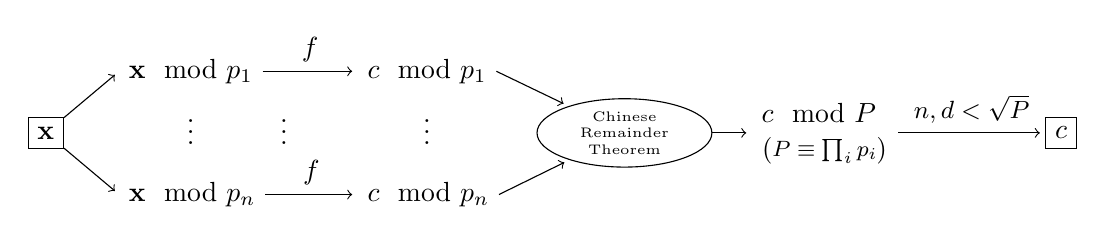
\begin{tikzpicture}[auto, node distance = 3cm,shorten >= 2pt]
      \node [rectangle, draw, text centered] (x) {$\mathbf{x}$};

      \node [above right = 0.3cm and 0.7cm of x] (xmod1) {$\mathbf{x}\mod p_1$};
      \node [right  of=xmod1] (cmod1) {$c\mod p_1$};

      \node [below right = 0.3cm and 0.7cm of x] (xmodn) {$\mathbf{x}\mod p_n$};
      \node [right  of=xmodn] (cmodn) {$c\mod p_n$};


      \node [below = 0cm of xmod1] () {$\vdots$};
      \node [below = 0cm of cmod1] () {$\vdots$};
      \node [below right = 0cm and 0.1cm of xmod1] () {$\vdots$};

      \node [ellipse, draw, text centered, right =6cm of x, node distance = 3cm, text width = 1.5cm, inner sep = 1pt] (crt) {\baselineskip=-10pt \tiny Chinese Remainder Theorem \par};
      \node [right = 0.5cm of crt] (cmodP) {\minibox{ $c\mod P$  \\ \footnotesize $\left(P\equiv\prod_i p_i\right)$} };

      \node [rectangle, draw, text centered, right of=cmodP, node distance = 3cm] (c) {$c$};


      \path [line,->] (x) -- (xmod1.west);
      \path [line,->] (x) -- (xmodn.west);

      \path [line,->] (xmod1.east) -- node [above]{$f$} (cmod1.west);
      \path [line,->] (xmodn.east) -- node [above]{$f$} (cmodn.west);

      \path [line,->] (cmod1.east) -- (crt);
      \path [line,->] (cmodn.east) -- (crt);

      \path [line,->] (crt) -- (cmodP);

      \path [line,->] (cmodP) -- node [above]{\small $n,d < \sqrt{P}$} (c);
    \end{tikzpicture}
  \end{center}
  \caption{The diagram representing rational reconstruction.}
  \label{fig:RatReconstr}
\end{figure}

\section{Solving Linear Systems of Equations}
For floating numerical stability is important.

For finite fields only field operations. PLU decomposition algorithm.

Put the one-loop cases here? Fourier transform and hard-coded solutions for inversions?

\section{On-Shell Loop Momenta and Finite Fields}
The extension of unitarity approaches to employ only operations
defined in an algebraic field was proposed 
in ref.~\cite{Peraro:2016wsq}.
A finite-field based calculation allows to compute exact values
for the integral coefficients $c_{\Gamma,i}$ of eq.~\eqref{eq:A}
in a numerical framework.
This idea
was applied recently in \cite{Badger:2017jhb,Abreu:2017hqn} for
pure gluon-scattering amplitudes, and here we discuss our
implementation for amplitude computations with fermions.

\subsubsection{Generic Algebraic Extension}

From here on we denote by $\mathbb{F}$ an arbitrary 
number field. In practice, we will be interested in
$\mathbb{F}$ being the field of rational numbers $\mathbb{Q}$
or the finite field $\mathbb{Z}_p$
of all integers modulo a prime number $p$.
In general, polynomial equations do not have solutions in 
$\mathbb{F}$. This is at odds with the fact that
in a unitarity-based approach one needs 
to generate loop momenta which satisfy a set of quadratic
conditions corresponding to setting propagators to zero.
%
In the presence of fermions, the situation becomes more 
complicated due to the extension of the Clifford algebra beyond 
four dimensions. More specifically, terms such as $\ell^\mu
\gamma_{[D_s]\mu}$ exhibit the $(D-4)$-dimensional
components of the loop momenta,
which are in general not 
$\mathbb{F}$-valued for on-shell momenta
(more concretely, if we work on the field of rational numbers
these components are in general irrational),
leading to terms in the sub-currents of the
Berends-Giele recursion that are not $\mathbb{F}$-valued. 
%
To address this issue,
we start with a parametrization of the on-shell spaces as in 
ref.~\cite{Abreu:2017hqn} but always use normalized basis
vectors. We write the two-loop momenta as
\begin{equation}
    \ell_1 = (\ell_{1,[4]}, \vec{\mu}_1)\,,\quad \quad \quad
    \ell_2 = (\ell_{2,[4]}, \vec{\mu}_2)\,, 
    \label{eq:loopmomenta}
\end{equation}
where we denote their $(D-4)$-dimensional components as 
$\vec{\mu}_1$ and $\vec{\mu}_2$. Next, we choose an orthonormal
basis $\vec{n}_i$ of the $(D-4)$-dimensional space with
$n_1$ in the direction of $\vec{\mu}_1$ and write
\begin{equation}
\vec{\mu}_1 = r_1 \vec{n}_1, \quad  \vec{\mu}_2 = \frac{\mu_{12}}{\mu_{11}} r_1 \vec{n}_1 + r_2 \vec{n}_2
  \quad \mathrm{where} \quad r_1 = \sqrt{\mu_{11}}, \quad r_2 = 
  \sqrt{\mu_{22} - \mu_{12}^2/\mu_{11}},
\end{equation}
with $\mu_{ij}=\vec{\mu}_i\cdot\vec{\mu}_j$.
In a theory containing only vector particles we only ever need 
the values $r_i^2$, which are $\mathbb{F}$-valued both on- and
off-shell \cite{Abreu:2017hqn}. In contrast, in a theory with
fermions, components of Berends-Giele currents will take the
generic form
\begin{equation}
  \label{eq:ExtendedAlgebra}
  a_{00} + a_{10} r_1 + a_{01} r_2 + a_{11} r_1 r_2, 
\end{equation}
which is not $\mathbb{F}$-valued.
In order to nevertheless be able to
work in the field $\mathbb{F}$,
we consider 
the algebra $\mathbb{V}$ over the field $\mathbb{F}$, with 
$\mathbb{V}$ the vector space spanned by the basis 
$\{r_0=1,r_1,r_2,r_1r_2\}$ and equipped with the standard
addition and multiplication.
All components of the Berends-Giele are elements 
in the algebra, and can thus be written as a linear combination
of the $r_i$ with $\mathbb{F}$-valued coefficients. More
concretely, this means we only need to determine the $a_{ij}$ 
in eq.~\eqref{eq:ExtendedAlgebra} which are $\mathbb{F}$-valued
by construction.

An important observation is that, although the coefficients 
$a_{10}$, $a_{01}$ and $a_{11}$ in 
eq.~\eqref{eq:ExtendedAlgebra} are non-zero in
intermediate stages of the calculations, they vanish
for the integrands of helicity amplitudes as defined in 
eq.~\eqref{eq:tensorDecomposition}. This cancellation of the
$r_i$ terms holds in the HV scheme and
is due to the projection onto the invariant tensors 
$v_n$ of eq.~\eqref{eq:tensorDecomposition}, 
which yields polynomials in the Lorentz invariants 
$\mu_{ij}$ at the integrand level
(see the discussion in section \ref{sec:ParamIntegrands}).


\subsubsection{Only Vector Particles}
%
In ref.~\cite{Abreu:2017hqn}, this was resolved
by making sure that all scalar products
between the momenta in the problem were $\mathbb{F}$-valued.


\subsubsection{Special Metric Signature}

Any Lorentz-invariant quantity such as helicity amplitudes (normalized by an appropriate spinor weight)
depends on the space-time metric tensor only through contractions with momenta and states of external particles.
Thus  without loss of generality we can choose to use an alternating metric signature $(+,-,+,-,\ldots)$
and modify external momenta such that all Lorentz invariants remain unchanged.

We then can parametrize the two-dimensional loop-momentum components
$\vec{\mu}_1$ and $\vec{\mu}_2$ as follows:
\begin{equation}
  \vec{\mu}_1(t)  = \frac{1}{2}\begin{pmatrix}
    t+\dfrac{\mu_{11}}{t} \\
    t-\dfrac{\mu_{11}}{t} \\
  \end{pmatrix}, \quad
  \vec{\mu}_2(t)  = \frac{\mu_{12}}{\mu_{11}}\vec{\mu}_1(t) - \frac{r}{\mu_{11}}~\frac{1}{2}\begin{pmatrix}
    t-\dfrac{\mu_{11}}{t} \\
    t+\dfrac{\mu_{11}}{t} \\
  \end{pmatrix},
  \label{eq:muparam}
\end{equation}
where $t$ is a free dimensionful parameter that leaves the scalar products
$r = \sqrt{\mu_{12}^2-\mu_{11} \mu_{22}}$ and 
$\mu_{ij} = \mu_i^1 \mu_j^1 - \mu_i^2 \mu_j^2$ invariant. %

This parametrization allows to reduce the size of the algebraic extension $\mathbb{V}$ generated by \cref{eq:ExtendedAlgebra},
which is a significant optimization of numerical evaluations.


\todo{Note on other possibilities to avoid solving on-shell conditions.}


\section{Exact Interpolation of Functions over Finite Fields}
\subsection{Univariate Polynomials}
\subsection{Multivariate Polynomials}




\chapter{Spinor-Helicity}
\label{chap:4dspinhel}

here describe four-dimensional spinor-helicity


%
%%% Literaturverzeichnis aus Datei "literatur"
%\phantomsection
%\nocite{apsrev41Control}
%\bibliography{zitationen,revtex-custom}
\bibliography{zitationen}

%
%%% Danksagungen aus Datei "src/danksag"
\chapter*{Acknowledgments\markboth{Acknowledgments}{}}
\addcontentsline{toc}{chapter}{Acknowledgments}
{
  \setlength{\parskip}{2pt}
  First of all, I would like to thank my first supervisor Harald Ita for his advice, guidance, fascinating insights
  and always giving me opportunities to grow as a researcher and giving me incentives to strive for higher standards.
  I am also very thankful to my second supervisor Fernando Febres Cordero for 
  being always ready to help me with all aspects of my doctoral studies,
  and letting me ask all the questions I ever wanted.
  I hope it was not too troublesome for you.

  I am very grateful to Ben Page and Samuel Abreu for patiently mentoring me,
  and very insightful discussions, research-related or otherwise.
  I cannot emphasize enough how valuable was it for me to have an opportunity to work by your side.

  I would like to thank my colleague Felix Anger, with whom I had worked closely in the first two years of my Ph.D.\ studies.
  It was a pleasure.

  My thanks go to Ekta Chaubey, Jerry Dormans, Michael Ruf, Wladimir Tschernow, Maximilian Klinkert, Harald Ita, Fernando Febres Cordero for critically reading parts of the manuscript and suggestions
  regarding the contents.

  I am also indebted to Ekta Chaubey for continuous encouragement, assistance, and for tolerating my complicated personality, especially during the time of writing this thesis. 

  I would like to thank Anna Gantimurova for supporting me in the first years of my doctoral studies.

  Finally, I would like to thank the ``Graduiertenkolleg 2044'' for providing a vibrant environment for carrying out Ph.D.\ research,   
  and for the unique opportunity of having a framework of dialogue with our colleagues from experiments. 

  %GRK for framework, seminars and events


  %%%%%%%

  %First and foremost I would like to thank my supervisor Harald Ita, for his scientific guidance and his supportive attitude. Your advice and help has been invaluable! I would also like to express my gratitude to my second supervisor Fernando Febres Cordero, for the good collaboration and his outstanding commitment. I really enjoyed working with you! 

  %I would like to thank my collaborators Stefan H{\"o}che and Daniel Ma{\^i}tre, for the things I have learnt from them.

  %I would like to thank my colleague and office mate Vasily Sotnikov, for all the discussions and good collaboration on many aspects of this work. We have been a good team! To all the current and former members of the 8\textsuperscript{th} (and 7\textsuperscript{th}) floor for supporting me in one or another way but also for the good times shared: Kicker tournaments, Christmas parties and the ``Betriebsausflug'' come to my mind. A special thanks goes to Samuel Abreu for reading the manuscript of this thesis, to Matthijs van der Wild for forming the winning team of the kicker tournament '17 and to Jerry Dormans for tolerating our long discussions in the office but also for the fun in ``office 809''. To the members of the $\hbar$-racing team for the shared memories on snow and beyond: Lukas Altenkamp, Michele Boggia, Michael Kordovan.

  %I would like to thank Hannah Arnold, Giulia Gonella and Gernot Knippen for the shared time as student representatives of the ``Graduiertenkolleg 2044''. From organizing BBQs to increasing the ``educational value'' of the seminar series: I think we provided some innovative impulses!
}

%


%
%%% Ende des Dokuments
\end{document}
